\documentclass[11pt,oneside]{book}

\usepackage[letterpaper,margin=1in]{geometry}
\usepackage[T1]{fontenc}
\usepackage[utf8]{inputenc}
\usepackage{lmodern}
\usepackage{microtype}
\usepackage{textcomp}
\usepackage{graphicx}
\usepackage{amsmath}
\usepackage{longtable}
\usepackage{booktabs}
\usepackage{array}
\usepackage{calc}
\usepackage{enumitem}
\usepackage{needspace}
\usepackage{fancyvrb}
\usepackage{upquote}
\usepackage[htt]{hyphenat}
\usepackage{xcolor}
\usepackage{xurl}
\usepackage[hidelinks,breaklinks=true]{hyperref}

\hypersetup{
  pdftitle={Engineering Reliable Coding Agents},
  pdfauthor={Stephanie Jarmak},
  pdfsubject={Evaluation, operation, and governance of AI coding-agent systems}
}

\setlength{\emergencystretch}{6em}
\setlength{\parindent}{1.25em}
\setlength{\parskip}{0.08\baselineskip plus 0.03\baselineskip minus 0.02\baselineskip}
\setcounter{secnumdepth}{2}
\setcounter{tocdepth}{1}
\makeatletter
\renewcommand*\l@section{\@dottedtocline{1}{1.5em}{3.3em}}
\makeatother
\setlist{
  topsep=0.62\baselineskip,
  partopsep=0.18\baselineskip,
  itemsep=0.16\baselineskip,
  parsep=0.04\baselineskip
}
\setcounter{topnumber}{3}
\setcounter{bottomnumber}{2}
\setcounter{totalnumber}{4}
\renewcommand{\topfraction}{0.90}
\renewcommand{\bottomfraction}{0.80}
\renewcommand{\textfraction}{0.08}
\renewcommand{\floatpagefraction}{0.72}
\setlength{\textfloatsep}{0.80\baselineskip plus 0.20\baselineskip minus 0.10\baselineskip}
\setlength{\intextsep}{0.80\baselineskip plus 0.20\baselineskip minus 0.10\baselineskip}
\setlength{\floatsep}{0.65\baselineskip plus 0.15\baselineskip minus 0.10\baselineskip}
\setlength{\abovecaptionskip}{0.45\baselineskip}
\setlength{\belowcaptionskip}{0.15\baselineskip}
\fvset{fontsize=\small}
\pagestyle{plain}

\providecommand{\tightlist}{%
  \setlength{\itemsep}{0.16\baselineskip}\setlength{\parskip}{0.04\baselineskip}}
\newcommand{\pandocbounded}[1]{%
  \begingroup
  \setbox0=\hbox{#1}%
  \ifdim\wd0>\linewidth
    \resizebox{\linewidth}{!}{\box0}%
  \else
    \box0
  \fi
  \endgroup}

\begin{document}
\frontmatter

\begin{titlepage}
  \centering
  \vspace*{0.16\textheight}
  {\Huge\bfseries Engineering Reliable Coding Agents\par}
  \vspace{1.2em}
  {\Large Evaluation, Recovery, Context, and Control Beyond the Model\par}
  \vspace{2.5em}
  {\large Stephanie Jarmak\par}
  \vfill
  {\large August 2026\par}
\end{titlepage}

\chapter*{Abstract}
\addcontentsline{toc}{chapter}{Abstract}
AI coding agents are commonly assessed as models but deployed as systems whose behavior also depends on evaluation harnesses, execution state, retrieval, permissions, review interfaces, and resource allocation. This technical monograph synthesizes evidence for engineering reliability at those system boundaries. Its evidence base comprises 118 scholarly sources organized into seven topic-specific review threads, 91 practitioner records, a 29-benchmark catalog, and 17 project dossiers. Evidence items are classified independently by source type and strength; a separate audit rechecks high-strength synthesis claims against underlying sources. From this corpus, two independent derivations produced a catalog of 192 bounded practices, of which 55 are developed in depth. The monograph contributes the evidence audit and practice catalog; a dependency chain connecting measurement, grading, containment and recovery, context, oversight, and allocation; scoped measurements and failure analyses from author-operated systems; and runnable protocols for local evaluation and fault testing. The synthesis is structured rather than exhaustive, capability results remain time- and workload-dependent, and evidence is uneven across topics. Author-system cases are therefore used as illustrations and are not treated as independent external evidence.


\tableofcontents
\chapter*{Introduction}
\addcontentsline{toc}{chapter}{Introduction}
\hypertarget{problem-and-scope}{%
\section{Problem and scope}\label{problem-and-scope}}

An agent has finished a change. The tests pass, and a reviewer is examining a compact diff. The run appears successful, yet the available record may not establish whether another run would produce the same result, whether the tests exercised the relevant behavior, or whether the reviewer saw the decisions that carried the most risk.

The visible output is code; the uncertainty around its quality resides in the system that produced, evaluated, and approved it. A coding agent is one component in that system. Evaluation determines what counts as success, governance constrains access, context management controls the information available during a run, review defines the quality gate, and scheduling allocates compute, money, time, and human attention.

These functions interact. A higher score can result from an easier test rather than a better system. A reviewer can appear ineffective because the interface concealed the evidence needed for judgment. Instrumentation can record component failures while missing failures at component boundaries. A recovery procedure can pass while depending on credentials whose compromise would also destroy the recovery path.

This technical review and engineering monograph examines the evaluation, operation, and governance of AI coding-agent systems. It focuses on mechanisms that remain relevant as models and products change: measurement design, execution-based grading, containment, durable state, recovery, repository retrieval, context limits, human oversight, topology, and resource allocation. It does not compare current models or teach prompt and tool-schema design.

The intended reader is a staff engineer, evaluation lead, or technical owner building a coding-agent evaluation or operations program. The statistical methods are introduced where they affect an engineering decision, but the monograph assumes comfort with experiment design, production controls, and technical review. Its practices are bounded engineering claims rather than universal rules. Their applicability depends on workload, permissions, failure costs, deployment conditions, and available review capacity.

\hypertarget{the-reliability-dependency-chain}{%
\section{The reliability dependency chain}\label{the-reliability-dependency-chain}}

The organizing argument is a dependency chain. Measurement determines whether a difference is credible. Grading converts observations into acceptance decisions. Containment and recovery determine whether the resulting execution record survives failure without extending authority. Retrieval and context determine which evidence reaches the agent. Review and accountability determine who can challenge the result and who controls the consequential transition. Allocation and cost determine which system receives future work.

Each layer determines what the next may trust. A weak measurement can become a confident grade; a weak grade can admit unsafe work; an incomplete recovery record can enter retrieval as if it were complete; missing context can make review appear ineffective; and an invalid review signal can steer more work toward the wrong configuration. Downstream confidence cannot repair evidence lost upstream.

This creates a repair asymmetry. Later machinery is often easier to add than the earlier instrument is to repair, yet it is evaluated through that earlier instrument. More samples cannot repair a task distribution that excludes production work. More judges cannot repair a rubric experts apply inconsistently. More agents cannot repair a retrieval boundary that treats an empty result as authoritative. The dependency chain is therefore a sequence of evidence obligations, not a list of subsystems.

\begin{figure}[htbp]
\centering
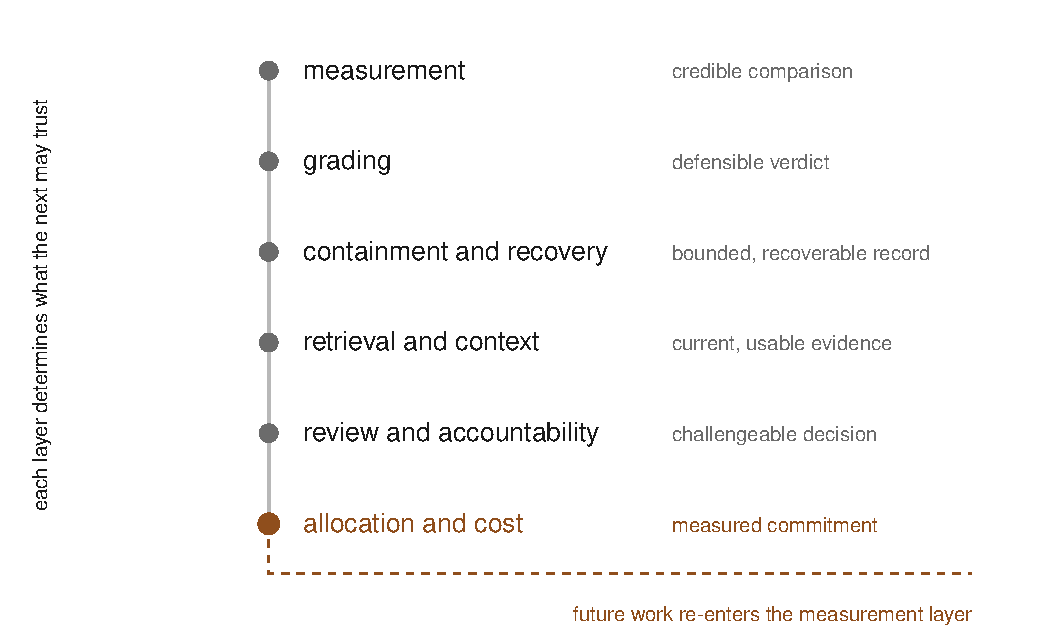
\includegraphics[width=1\textwidth,height=\textheight,keepaspectratio]{figures/dependency-chain.pdf}
\caption{Argument map for the reliability dependency chain: measurement, grading, containment and recovery, retrieval and context, review and accountability, and allocation and cost. Each layer supplies the evidence boundary on which the next relies.}
\end{figure}

The six parts follow this order. It is not a progression from easy to difficult. It is an account of how an apparently local defect can propagate into later operational decisions while retaining the appearance of a clean score, verdict, or artifact.

\hypertarget{method-scope-and-evidence-classification}{%
\section{Method, scope, and evidence classification}\label{method-scope-and-evidence-classification}}

This review treats source collection, evidence grading, practice derivation, and the treatment of author-system cases as separate methodological decisions. The following subsections describe each decision and the limits it places on the resulting claims.

\hypertarget{search-and-source-assembly}{%
\subsection{Search and source assembly}\label{search-and-source-assembly}}

The review was consolidated on July 26, 2026, then subjected to a bounded update audit and a software-engineering venue coverage probe through August 6, 2026. The release-candidate source collection contains 138 scholarly works, 91 practitioner records, 29 benchmark records, and 17 author-system case records. The original 118 scholarly works were organized into seven topic-specific threads covering benchmark validity, failure taxonomy, evaluation statistics, oversight and accountability, context and retrieval, durable execution, and scheduling with repository-scale scoping. Eleven works were admitted during the update audit and nine during the coverage probe.

Scholarly retrieval used \href{https://scixplorer.org/scixabout/}{SciX}, the NASA-supported literature discovery service operated by the Smithsonian Astrophysical Observatory, and a local retrieval layer referred to here as \textbf{SciX Agent}. The official \href{https://scixplorer.org/scixhelp/api-scix/}{SciX API} supplied bibliographic identities and metadata. At consolidation, SciX Agent searched a 32.4-million-record SciX and arXiv corpus with 299.3 million citation links and full text for 14.9 million records. It combined INDUS dense retrieval with BM25 lexical retrieval through reciprocal-rank fusion. These systems determined which records were retrieved and read first; they did not determine evidence grades.

Queries were scoped by topic, subject class, and year where appropriate. Each thread combined seminal work with recent agent-era research. Candidate records were verified by identity, and full text was read when available and when the claim required more than the abstract. A citation audit added the seventh thread after finding scheduling and repository-scoping sources that had entered the draft through adjacent operations-research material.

Practitioner retrieval used the \textbf{\href{https://www.sjarmak.ai/projects/code-intelligence-digest}{Code Intelligence Digest}}, an author-operated corpus that ingests research feeds, engineering publications, newsletters, podcasts, community discussions, and product or operations accounts. At the July 26 cutoff, its local snapshot contained 162,350 normalized records from 149 source labels, including 43,953 records with retained full text. Keyword and semantic retrieval were used within relevant practitioner categories. Research records found through the Digest were moved to the scholarly lane and deduplicated there. Repeated practitioner accounts of one incident shared an independence key and could not be counted as independent corroboration merely because several pages repeated the event.

This practitioner lane makes the review \textbf{multivocal} in the software-engineering sense described by Garousi, Felderer, and Mäntylä (\href{https://doi.org/10.1016/j.infsof.2018.09.006}{2019}): it combines scholarly and grey literature because operational mechanisms and incidents are often documented outside venues. The lane also follows the more restrictive point made by Kitchenham and colleagues (\href{https://doi.org/10.1109/TSE.2022.3165938}{2022}): a mutable social-media post is not treated as a primary study merely because it is informative. Practitioner records remain corroborating cases unless they report a sufficiently specific measurement, and mutable cited pages are archived. The independence key operationalizes source independence by grouping reports that repeat one originating incident or claim.

The benchmark collection was assembled separately from benchmark documentation and publications, merged from two inventories, deduplicated by identity, and validated against a JSON Schema. Three repeated benchmark records were removed during that merge.

The initial scholarly search did not establish adequate coverage of the core software-engineering venue literature. A subsequent OpenAlex metadata probe searched eight topic formulations across ICSE, FSE, ASE, ISSTA, \emph{Empirical Software Engineering}, \emph{IEEE Transactions on Software Engineering}, \emph{ACM Transactions on Software Engineering and Methodology}, and \emph{Computer Supported Cooperative Work}. It surfaced 148 unique candidates. Nine methodologically material works were admitted after title-and-abstract screening, including the SEGRESS reporting guideline (\href{https://doi.org/10.1109/TSE.2022.3174092}{Kitchenham et al.~2022}), the ABC framework for software-engineering research (\href{https://doi.org/10.1145/3241743}{Stol and Fitzgerald 2018}), and work on construct validity in software engineering (\href{https://doi.org/10.1109/TSE.2022.3176725}{Sjøberg and Bergersen 2023}).

That probe diagnosed coverage; it did not replace a publisher-native search. In a deterministic sample of 40 candidate DOIs, SciX contained eight exact DOI matches. The sample is too small and topical to estimate corpus recall, but the missing records are sufficient to reject an assumption of complete SE venue coverage. ACM Digital Library returned HTTP 403 to the automated search client, while the IEEE Xplore and Scopus APIs required credentials not configured in the review environment. The archival first edition is therefore conditional on a supplementary search executed against ACM Digital Library, IEEE Xplore, and Scopus, or on a documented database substitution whose coverage is justified. The companion preserves the probe protocol, all 148 candidates, and the exact SciX comparison.

\begin{figure}[htbp]
\centering
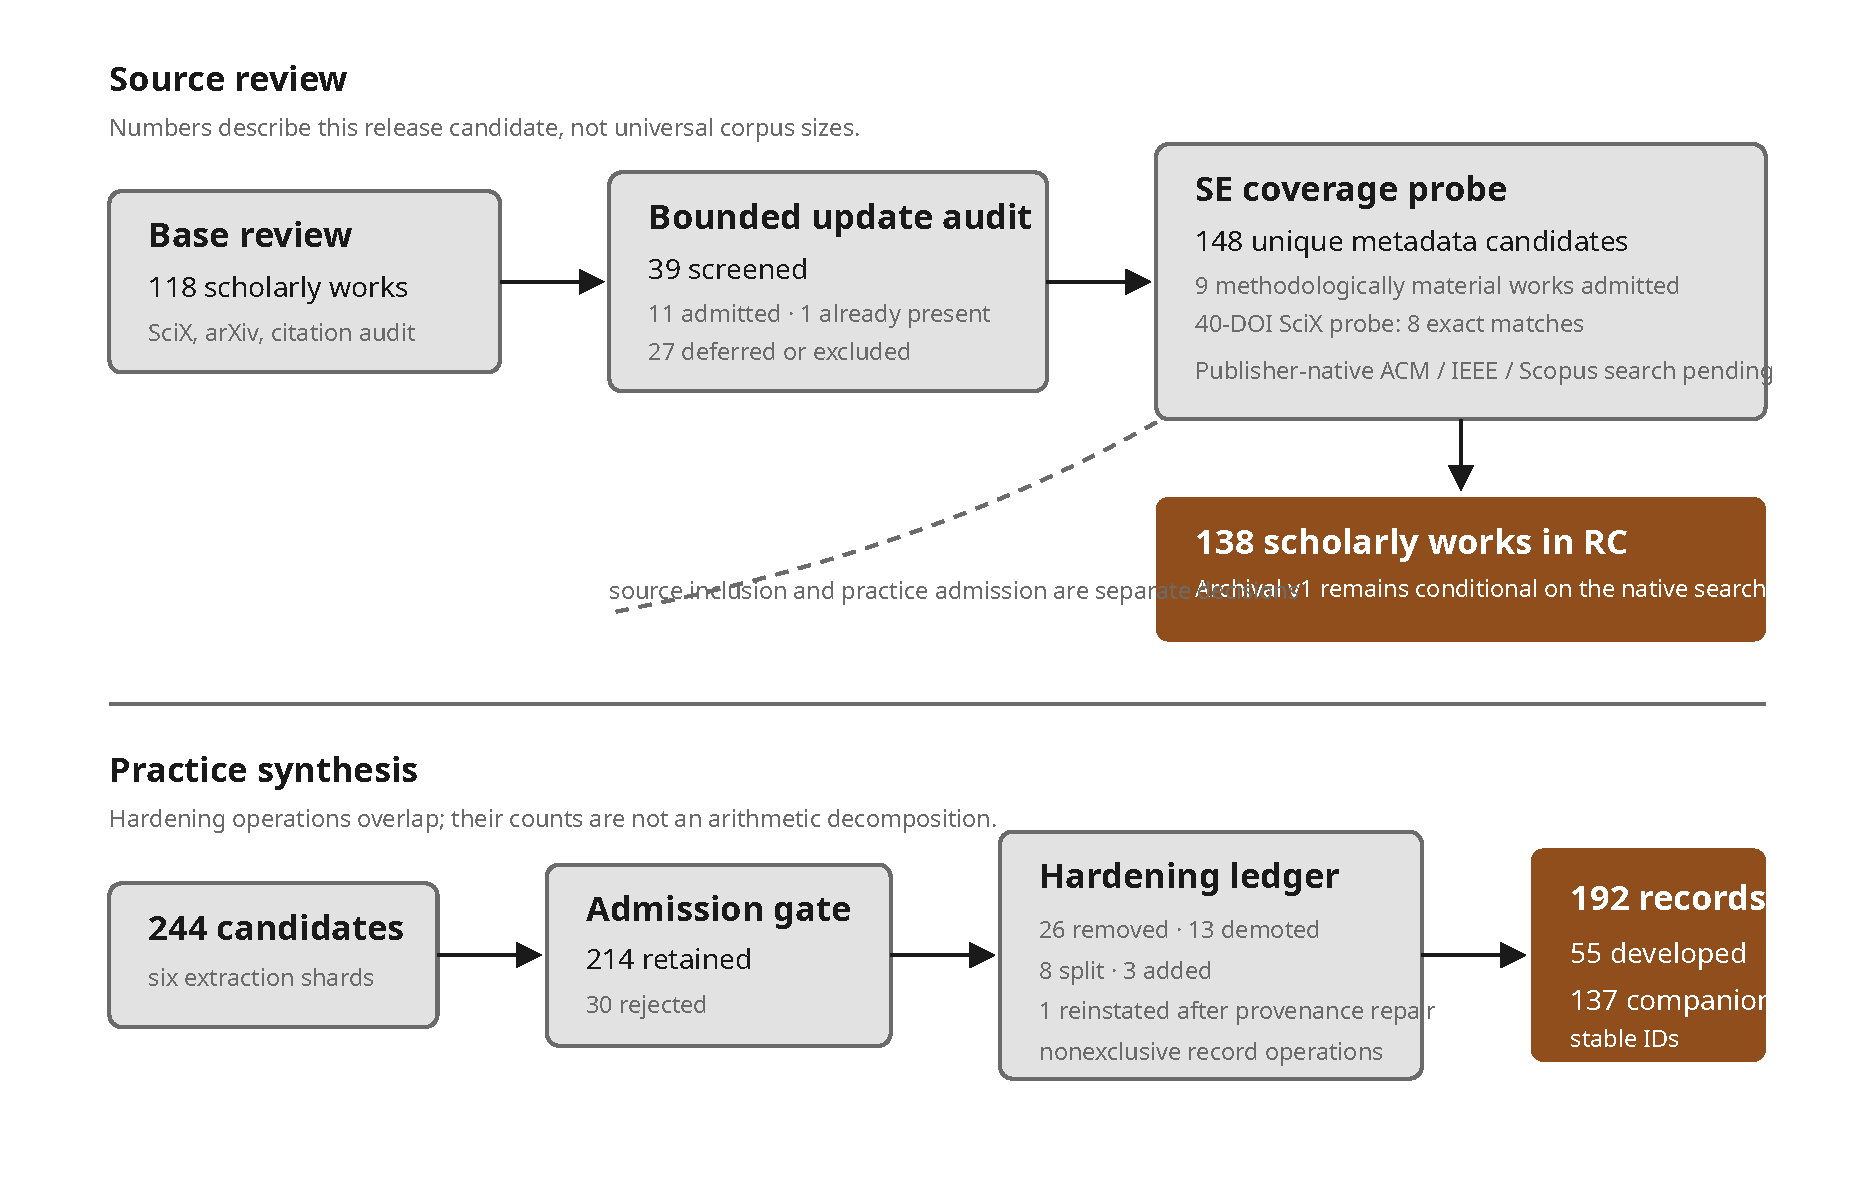
\includegraphics[width=1\textwidth,height=\textheight,keepaspectratio]{figures/review-flow.pdf}
\caption{Flow of source review and practice synthesis. The source lane distinguishes the base review, bounded update audit, SE coverage probe, and the remaining publisher-native search. The practice lane reports the admission gate and overlapping hardening operations without treating their counts as an arithmetic decomposition.}
\end{figure}

The search remains structured rather than exhaustive. It does not cover every scholarly index, venue, private operational record, or adjacent model-comparison literature. The SEGRESS reporting items provide the vocabulary used below: source admission is governed by inclusion and exclusion criteria; evidence-group assignment is a quality assessment of a scoped claim; and practice construction is data extraction and synthesis. These names do not change the underlying decisions, but they make the review easier to compare with software-engineering secondary studies.

\hypertarget{curation-and-assembly-workflow}{%
\subsection{Curation and assembly workflow}\label{curation-and-assembly-workflow}}

The assembly process followed a fixed sequence: define a question for each thread; retrieve candidates; resolve record identity; screen for an in-scope claim; extract the bounded claim and its conditions; assign an evidence group; challenge the assignment; derive candidate practices; select practices for chapter treatment; and audit the final citations. Retrieval rank determined screening order only. A highly ranked record received no evidentiary preference after screening.

Automated systems assisted with retrieval, normalization, duplicate detection, bounded claim extraction, metadata checks, and challenge passes. The cited source remained authoritative. The author made the final decisions about inclusion, evidence grouping, practice admission, chapter placement, and prose. When a challenge pass exposed ambiguity, the lower evidence group was used unless the narrower strong claim could be stated directly.

\begin{longtable}[]{@{}
  >{\raggedright\arraybackslash}p{(\columnwidth - 4\tabcolsep) * \real{0.3333}}
  >{\raggedright\arraybackslash}p{(\columnwidth - 4\tabcolsep) * \real{0.3333}}
  >{\raggedright\arraybackslash}p{(\columnwidth - 4\tabcolsep) * \real{0.3333}}@{}}
\caption{Automation and human judgment in the review workflow. \emph{Automated} means the operation ran without item-level prompting; \emph{assisted} means a system proposed or flagged material for a human decision; \emph{human} means the substantive choice was made without an automated verdict.}\tabularnewline
\toprule\noalign{}
\begin{minipage}[b]{\linewidth}\raggedright
Review step
\end{minipage} & \begin{minipage}[b]{\linewidth}\raggedright
Mode
\end{minipage} & \begin{minipage}[b]{\linewidth}\raggedright
Human decision retained
\end{minipage} \\
\midrule\noalign{}
\endfirsthead
\toprule\noalign{}
\begin{minipage}[b]{\linewidth}\raggedright
Review step
\end{minipage} & \begin{minipage}[b]{\linewidth}\raggedright
Mode
\end{minipage} & \begin{minipage}[b]{\linewidth}\raggedright
Human decision retained
\end{minipage} \\
\midrule\noalign{}
\endhead
\bottomrule\noalign{}
\endlastfoot
Candidate retrieval and ranking & Automated and assisted & I defined each thread question and search boundary, then read the admitted sources. \\
Identity resolution, normalization, and duplicate checks & Automated checks with human resolution & I resolved ambiguous identities and practitioner independence keys. \\
Bounded-claim extraction & Assisted & I checked the source, revised the extracted claim, and accepted or rejected it. \\
Initial evidence-group proposal & Assisted & I assigned the final label to the scoped claim. \\
Challenge pass & Assisted & Automated passes flagged composite claims, contrary findings, duplicate support, and label inconsistencies; I reread the source and adjudicated each change. \\
Practice admission, chapter selection, and prose & Human & I made the selection and writing decisions. \\
Schema, checksum, identifier, and cross-reference gates & Automated verification & A failure blocked the release until the underlying record was corrected. \\
\end{longtable}

The challenge pass was an error-finding aid, not an independent grader. In particular, automated assistance in that pass searched for composite claims, inconsistent evidence groups, contrary findings, duplicate support, and broken identifiers. It did not accept a practice or promote an evidence group.

The update audit screened 38 distinct scholarly records surfaced in Code Intelligence Digest editions published from July 27 through August 5, plus one paper found in a targeted August 6 check. Eleven new works were admitted, one record was already present, and 27 were deferred or excluded. Admission required a material addition to a claim already in scope; novelty or recency alone was insufficient. Material published after August 6 enters the update queue for a later edition unless it corrects a factual error in this one.

Working thread syntheses and source receipts were retained, but the original interactive searches did not preserve every machine-issued query in a publication-ready log. The companion therefore distinguishes retained records from reconstructions. It publishes the source snapshots, sanitized thread protocols, the retained update-search record, and record-level update decisions; it does not present reconstructed query text as an exact historical log. This permits protocol-level review without implying that every interactive search can be replayed byte for byte.

\hypertarget{screening-and-evidence-grading}{%
\subsection{Screening and evidence grading}\label{screening-and-evidence-grading}}

A source entered the working corpus when it contributed at least one measured result, reproducible mechanism, operational incident, benchmark property, or concrete practice relevant to coding-agent reliability. Screening removed records with unresolved identity, no recoverable claim, no relation to a decision in scope, or complete redundancy with a better-supported record. Sources could remain in the review while a proposed practice was rejected; source inclusion and practice admission were separate decisions.

\Needspace{5\baselineskip}

Evidence is reported in four reader-facing groups:

\begin{itemize}
\tightlist
\item
  \textbf{Strong evidence} is an on-claim controlled comparison, validated benchmark result, or comparably specific measurement within stated conditions.
\item
  \textbf{Directional evidence} supports a mechanism, threat model, comparison design, or direction of effect without establishing the complete recommendation, its magnitude, or broad transfer.
\item
  \textbf{Corroborating evidence} consists of case reports, practitioner accounts, or convergent observations that establish plausibility without estimating prevalence.
\item
  \textbf{Null or conflicting evidence} records a result that did not support the expected effect or that materially limits another claim.
\end{itemize}

These labels attach to evidence items and scoped claims, not to publication venues or whole chapters. A composite recommendation does not become strong because several directional sources converge. When no individual controlled study supports the complete recommendation, the text either narrows the claim to the measured component, classifies the transfer as directional, or presents a protocol to test locally. A strong item may therefore support one step of a developed practice while leaving the generalized prescription directional.

The catalog was graded during assembly and then challenged through independent verification passes. A targeted audit examined ten practices whose sole supporting synthesis had been graded strong, together with two restored items. Six grades were reduced because the source demonstrated a hazard, substrate, or adjacent result rather than the stated remedy; six were retained because the controlled comparison matched the claim. Identifier checks, duplicate-identifier gates, thin-evidence rulings, practitioner-independence checks, and contrary evidence were preserved in the audit record. Ambiguous cases defaulted to the lower grade.

The final adjudication was performed by the author. The challenge passes reduced correlated review error, but they do not constitute blinded independent grading by several human reviewers. That creates an asymmetry with Chapter 5, which asks operators to calibrate graders against independent labels before relying on them.

The release artifact therefore includes a deterministic random sample of 20 practices, the associated evidence items with the author's labels hidden, a reviewer response template, and a script that reports pairwise Cohen's kappa, Fleiss's kappa when three readers participate, observed agreement, and disagreement patterns. At least two external readers must complete that pass before archival v1. This release candidate reports no agreement value because no external labels have yet been collected. The author label will be compared after the blinded pass and will not be treated as ground truth. Even after calibration, agreement measures reproducibility of the quality-assessment instrument rather than correctness of every grade.

\hypertarget{practice-derivation-and-chapter-selection}{%
\subsection{Practice derivation and chapter selection}\label{practice-derivation-and-chapter-selection}}

Candidate practices were derived through bounded-claim extraction and synthesis, then passed through a separate admission gate. A record qualified at the final gate through at least one scholarly item, a non-author synthesis with a resolvable scholarly identity, or at least two practitioner items with distinct independence keys. Hardening separated bundled claims, removed redundant or self-defeating records, preserved contrary findings, and repaired provenance. The resulting catalog contains 192 edition records, each with a stable identifier. That total reflects the chosen claim granularity and editorial boundaries; it is not an estimate of how many reliability practices exist. The companion preserves the full record arithmetic and identifies which hardening operations overlap.

Three selection passes ranked the catalog by different criteria: teachability through a bounded case, consequence for an engineering decision, and coverage of the fourteen mechanism clusters. Practices selected by at least two passes formed the base of the developed set. Individual adjudication then repaired thin mechanism coverage and one provenance defect. The resulting 55 practices receive full treatment in the 18 chapters; the remaining 137 appear in the companion catalog.

The consequence ranking also supplies the operational-urgency calculation used later in the monograph. Among its 52 ranked practices, the Spearman correlation between urgency rank and a binary indicator for whether the practice carried at least one strong evidence item was -0.004. The phrase \emph{nearly uncorrelated} refers to this calculation, not to all 192 catalog entries or to a latent universal measure of importance.

The resulting chapter set is an authorial engineering judgment, not an evidence-derived consensus. The near-zero correlation makes that distinction visible. Some practices are included because a controlled comparison measured their effect; others are engineering controls justified by a structural failure mechanism, an observable check, and an asymmetric cost of waiting for trial evidence. Separating a recovery identity from a production identity, for example, can be tested directly against the authority boundary even when no study estimates how often shared credentials cause loss. Imperative section titles name the control or observation to implement; they do not imply a universal effect size or settled prevalence estimate. Where the argument is mechanistic rather than experimental, the chapter supplies a local test and avoids a numerical target.

\hypertarget{author-system-cases-and-limitations}{%
\subsection{Author-system cases and limitations}\label{author-system-cases-and-limitations}}

Cases from systems operated by the author expose mechanisms, original measurements, and reproducible failure cases. They are always treated as illustrations or local measurements. They are not counted as independent external evidence and do not by themselves support a general recommendation.

A \textbf{local artifact} is a record from a system operated by the author and used to expose a mechanism or local measurement. It is not independent external evidence. When its source was uncommitted at the cited revision or its figures were read from source rather than independently remeasured, the chapter states that provenance condition at first use instead of assigning the artifact a second name.

Evidence remains uneven across topics. Several operational questions have only case-level support, recent capability measurements can age quickly, and practitioner reports are vulnerable to selection, survivorship, and reporting bias. The review excludes model-comparison and prompt-engineering literatures except where they bear directly on system reliability. Transfer is especially substantial in Part VI, where observatory scheduling, compute-cluster scheduling, and adjacent multi-agent studies motivate testable designs for coding-agent fleets. That part should be read partly as a research agenda, not as a body of settled deployment guidance.

This section establishes the standard evidence legend for the whole monograph. Later chapters repeat a limitation only when it changes how a particular result may be used.

\hypertarget{contributions}{%
\section{Contributions}\label{contributions}}

\Needspace{5\baselineskip}

This work makes six contributions:

\begin{enumerate}
\def\labelenumi{\arabic{enumi}.}
\tightlist
\item
  a multivocal evidence audit and machine-readable ledger that distinguish direct support, directional findings, corroborating cases, and null or conflicting results;
\item
  a versioned catalog of 192 bounded practice records in this edition, including 55 developed in depth and stable identifiers that connect the manuscript, companion, and implementation artifacts;
\item
  a dependency chain---and its repair asymmetry---connecting measurement, grading, containment and recovery, context management, human oversight, and resource allocation;
\item
  original measurements and failure cases from author-operated systems, explicitly separated from external evidence;
\item
  runnable protocols for local evaluation, capability-boundary testing, recovery testing, trace analysis, and release decisions; and
\item
  five reusable agent skills with practice-level evidence maps, packaged in the project repository as implementation artifacts rather than additional evidence.
\end{enumerate}

The chapters emphasize conditions, measurements, and failure boundaries because an outcome alone rarely identifies why a system succeeded or failed. A useful account traces ownership, permissions, persistence, ordering, and observation while distinguishing correctness from reliability, performance, cost, safety, and usability.

\hypertarget{a-minimum-pass-through-the-dependency-chain}{%
\section{A minimum pass through the dependency chain}\label{a-minimum-pass-through-the-dependency-chain}}

\Needspace{5\baselineskip}

For an existing system, one compact pass produces the minimum record on which later decisions can build:

\begin{enumerate}
\def\labelenumi{\arabic{enumi}.}
\tightlist
\item
  Reopen one decision based on an aggregate score. Run the cheapest credible baseline and the candidate on identical task versions, initially three times per item, and preserve per-item outcomes.
\item
  Record success, reliability, cost, latency, model, harness, prompt, permissions, and pricing snapshot separately.
\item
  Exercise one permitted and one prohibited action with the ordinary identity, including the boundary between primary and recovery resources.
\item
  Verify one recent completion claim from repository or system state and rerun the executable check that makes it true.
\item
  Read twenty failed or unverifiable runs, label the first upstream failure where the trace permits it, and repair the first ordinary causal question the schema cannot answer.
\item
  Before the next promotion run, record the success floor, cost ceiling, task and baseline versions, mechanism condition, and fault-containment guard.
\end{enumerate}

The pass leaves six challengeable artifacts: a paired distribution, a cost-quality record, an observed authority boundary, an independently verified state transition, a seed failure corpus, and a decision rule fixed before the result was known. It is an entry point, not a reliability certificate. The repository artifact \href{https://github.com/sjarmak/engineering-reliable-coding-agents/blob/main/protocols/minimum-reliability-pass.md}{\texttt{protocols/minimum-reliability-pass.md}} supplies the runnable checklist and retained-artifact layout; the chapters develop each step.

\hypertarget{how-the-monograph-is-organized}{%
\section{How the monograph is organized}\label{how-the-monograph-is-organized}}

The monograph has six parts and eighteen chapters. Measurement comes first because every later practice is adopted or rejected through a measured comparison. Nineteen developed practices in Parts II through VI also require a method introduced in Part I. Interleaving those methods with their uses would scatter each method across four or five chapters.

This order places three chapters of experiment design before the agent-specific operating chapters. Later recommendations depend on those definitions and comparison methods.

Part I establishes how I compare systems when runs vary and scores can mislead. Part II turns those measurements into grading and release decisions. Part III addresses containment, persistent state, recovery, and failure analysis. Part IV examines how repository information enters, survives, and leaves an agent run. Part V treats human review as an engineered control with interfaces, escalation rules, and accountable ownership. Part VI is a research agenda for allocating work across agents and models under cost and capacity constraints. Its questions transfer methods from adjacent scheduling and multi-agent literatures rather than presenting settled coding-agent effects.

\begin{longtable}[]{@{}
  >{\raggedright\arraybackslash}p{(\columnwidth - 4\tabcolsep) * \real{0.3000}}
  >{\raggedleft\arraybackslash}p{(\columnwidth - 4\tabcolsep) * \real{0.4000}}
  >{\raggedright\arraybackslash}p{(\columnwidth - 4\tabcolsep) * \real{0.3000}}@{}}
\caption{Parts and chapters in the dependency-chain order.}\tabularnewline
\toprule\noalign{}
\begin{minipage}[b]{\linewidth}\raggedright
Part
\end{minipage} & \begin{minipage}[b]{\linewidth}\raggedleft
Ch
\end{minipage} & \begin{minipage}[b]{\linewidth}\raggedright
Title
\end{minipage} \\
\midrule\noalign{}
\endfirsthead
\toprule\noalign{}
\begin{minipage}[b]{\linewidth}\raggedright
Part
\end{minipage} & \begin{minipage}[b]{\linewidth}\raggedleft
Ch
\end{minipage} & \begin{minipage}[b]{\linewidth}\raggedright
Title
\end{minipage} \\
\midrule\noalign{}
\endhead
\bottomrule\noalign{}
\endlastfoot
\textbf{Part I: Evaluation measurement and experiment design} & 1 & Run-to-run variance, statistical power, and paired comparisons \\
& 2 & Baselines, ablations, and cost-accuracy tradeoffs \\
& 3 & Benchmark contamination, oracle strength, and workload validity \\
\textbf{Part II: Evaluation and grading systems} & 4 & Execution-based evaluation, correction gates, and release tests \\
& 5 & Calibrating model graders and separating agreement from correctness \\
& 6 & Proxy metric gaming and layered evaluation signals \\
\textbf{Part III: Containment, durable execution, and recovery engineering} & 7 & Agent isolation, injection defenses, and independent verification \\
& 8 & Persistent agent state, durable workflows, and idempotent retries \\
& 9 & Replayable traces and fault-injection recovery testing \\
& 10 & Human-auditable failure analysis and taxonomy development \\
\textbf{Part IV: Context engineering: retrieval, budgets, and memory} & 11 & Measuring and designing repository retrieval \\
& 12 & Localization funnels, repository indexes, and freshness checks \\
& 13 & Usable context budgets, consolidated-spec restarts, and file-based tool output \\
& 14 & Cross-session memory, raw traces, and compaction policies \\
\textbf{Part V: Human review and accountability engineering} & 15 & Efficient verification interfaces and risk-based human escalation \\
& 16 & Autonomy calibration, provenance, effective gates, and accountability \\
\textbf{Part VI: Research agenda---work allocation and cost engineering} & 17 & Agent topology selection and dynamic task allocation \\
& 18 & Cost-aware fleet scheduling and model routing \\
\end{longtable}

\hypertarget{what-i-assume-you-know}{%
\section{What I assume you know}\label{what-i-assume-you-know}}

I assume working knowledge of version control, continuous integration, code review, on-call practice, containers, and basic statistics. I use those foundations without rebuilding them. I still describe the relevant system boundary when a familiar tool plays an unfamiliar role.

I assume no prior exposure to the evaluation methods specific to public agent results. I begin with how to read a public score and identify the claim it can support. I then show how many repeated runs a comparison needs before an observed difference carries useful information. The answer depends on variation and the size of the difference you need to detect.

I also teach why agreement with human labels does not by itself make an automated grader correct. Agreement can conceal shared mistakes, ambiguous examples, or a reference answer that measures the wrong property. I separate the observed agreement from the inference made about correctness, which becomes important when a grader controls release.

Another method checks whether a score was earned on work the model had already encountered. I introduce the required vocabulary only when the mechanism appears. My goal is that a technically capable reader should be able to reproduce the reasoning presented in this monograph, not merely accept my interpretation.

The monograph does not assume a particular agent architecture or deployment scale. I describe architecture separately from implementation so the mechanism survives changes in products and interfaces. Examples expose permissions, retries, caching, concurrency, identity, and ordering when those details affect the claim. Code appears only when prose would obscure a state transition or failure path.

\hypertarget{how-to-read-a-chapter}{%
\section{How to read a chapter}\label{how-to-read-a-chapter}}

A chapter opens on a concrete situation, usually a measurement that came out wrong or a failure with a traceable cause. The mechanism follows, then what the evidence does and does not establish, then the boundary conditions, then a procedure you can run. Specialized terms are marked in bold where they are defined, so a term met later can be traced back to that site.

Citations appear inline in author-year form, with the year linked to the source. The back matter of each chapter, headed Sources and evidence, records the evidence grouping, identifier, and claim supported by each item. The back matter is authoritative for identifiers and evidence grouping; the prose states the claim for which a source is used. A disagreement between the two is an editorial defect.

The evidence legend in the methods section applies throughout. Chapter text restates only limitations that materially narrow a particular result, while each unnumbered Sources and evidence section records the claim, identifier, and evidence group for the cited items.

\hypertarget{the-companion-catalog}{%
\section{The companion catalog}\label{the-companion-catalog}}

The \href{https://sjarmak.ai/books/engineering-reliable-coding-agents/companion}{companion site} indexes all 192 practices under the chapter whose mechanism each extends. The 55 developed in the main chapters appear as short pointers into the chapter; the remaining 137 appear as compact entries. The catalog broadens the set of available options without forcing the main text to explain every variation. The \href{https://github.com/sjarmak/engineering-reliable-coding-agents}{project repository} contains the versioned manuscript, evidence ledger, benchmark catalog, schemas, provenance data, and release checksums. The \href{https://sjarmak.ai/books/engineering-reliable-coding-agents}{web edition} provides the browser-oriented reading version.

Use the relevant chapter as the foundation, then consult the catalog for practices that match a specific constraint. A compact entry cannot reproduce the chapter's full treatment of mechanism, evidence, tradeoffs, and failure boundaries. The chapter provides the reasoning needed to decide whether a neighboring practice applies to your workload.

Twenty-nine of the full entries are labeled as limited-support notes. I excluded them from the developed set because the available evidence does not support a recommendation. Treat them as prompts for investigation rather than established guidance. They may point to a useful experiment, a missing control, or a failure mode worth instrumenting.

The chapters and catalog serve different purposes. The chapters develop methods and claims in enough detail to evaluate critically. The catalog preserves breadth and makes related practices easier to find. Together, they let you begin with a measured problem and identify an intervention suited to the system you actually operate.

The repository also packages five reusable agent skills derived from selected practices: evaluation design, end-to-end test design, failure-mode capture, focused execution, and verified long-running implementation. Each skill includes a practice-level evidence map. These are implementation artifacts intended to make the protocols reusable; they are not additional evidence that the practices work across environments.

This edition is versioned because capability measurements and source availability change. The evidence ledger is scheduled for an annual review, with an out-of-cycle release when a material factual error, citation failure, or retraction changes a claim. Stable practice IDs persist across those releases; a later edition may retire, split, or merge a record without silently reusing its identifier.

\hypertarget{what-you-should-be-able-to-do-by-the-end}{%
\section{What you should be able to do by the end}\label{what-you-should-be-able-to-do-by-the-end}}

Given a published agent score, you should be able to state the narrower claim it supports and identify the conditions on which that claim depends. Given a proposed change to your own system, you should be able to measure run-to-run variation before crediting a difference and size the comparison before spending the model calls. Both systems should run on the same items, and a design that cannot resolve the difference relevant to the decision should return no verdict. Cost belongs in that judgment alongside accuracy, as does the possibility that a simpler configuration would have performed just as well.

You should be able to assess whether a public score was earned on tasks the model may already have encountered and to build an evaluation set from your own repositories when the public benchmark does not represent your work. Grades should rest on execution rather than the model's confidence, and automated graders should be validated against human labels before they gate releases. When a proxy improves without a corresponding improvement in the outcome it represents, the system should make that divergence visible.

Operationally, you should be able to bound what a single run can access and destroy, and you should treat an agent's account of its own work as a claim that still requires verification. A run that fails partway through should leave a durable record of which steps completed, and every retried step should be safe to execute again. Recovery should be tested by injecting failures rather than inferred from an architecture diagram. Reading a hundred traces from your own system should yield a concrete failure taxonomy.

Retrieval should be evaluated separately from generation so that a wrong answer can be attributed to the stage that produced it. You should also be able to measure how much of an advertised context window the system can use effectively. Human review should occur where the reviewer can see the decision that carries the risk, and autonomy should expand by action type only when measured approval and modification rates justify it. A multi-agent design should be required to outperform a single agent on the same tasks, and each component should run on the least expensive model that can perform its role reliably.

The goal is to provide you with the tools to measure what matters for your work, so the result describes the system you operate rather than a position on a leaderboard.


\mainmatter
\part{Evaluation measurement and experiment design}

\chapter{Run-to-run variance, statistical power, and paired comparisons}
\label{ch01-variance-power-paired-comparisons}
\section{One run is one draw}\label{one-run-is-one-draw}

I created an evaluation tool called CodeProbe (\href{https://github.com/sjarmak/codeprobe}{public repository}) that mines tasks from a repository's merged pull requests. In one of my runs using the tool it had reported that one configuration led another by +0.054 on a task family, and a single task accounted for most of that gap with a +0.300 advantage. This seemed reasonable, nothing about the run was `wrong', and the scoring code returned a number precise to three decimal places. I could easily have written the larger score up as a win.

But, in my stubborn scientific ways, I reran the family instead, three times per configuration. The difference fell to +0.0035, with a 95\% \textbf{confidence interval}, the range produced by a procedure that covers the true value in 95\% of repeated experiments, running from -0.0005 to +0.0074. The five tasks in the family were the paired units: the three repeats collapsed into one per-configuration score for each task, leaving five paired observations and 4 degrees of freedom. The paired t statistic of 2.41 fell below the critical value of 2.776, so the result was the semi-dreaded `not significant'. The task that had appeared to improve by +0.300 came back at exactly 0.000, with both configurations scoring 0.800 on every repeat.

Those reruns showed that the original observation could not justify a claim that would have been easy to make. One bad baseline score created the outlier, and the outlier disappeared once the trial was repeated. Three decimal places of `precision' is meaningless with a single run, and it describes the format of the number while indicating nothing about the stability of the process that produced it.

This task family scores through a deterministic test-suite oracle, under which the end state either passes the fixed tests or does not. That oracle collapses different trajectories onto the same score, so the tight repeat scores are a certification of scorer stability rather than agent determinism. The conclusion covers these five fixed tasks and no wider population.

It is critical to record repeated independent runs before declaring a meaningful difference between agent systems. A single score is one outcome from a variable execution process, even when the configuration appears deterministic. Without repeats, the observed difference mixes the system change I intended to test with variation from model execution, infrastructure, task ordering, and the other choices built into the evaluation apparatus.

Agent evaluations usually arrive as a table with one row per system and one score per row, which suppresses the execution history behind each cell. A score can aggregate hundreds of tasks and still be a single run, if each task was attempted once under one instantiation of the surrounding conditions.

Each cell has three layers behind it. A public agent benchmark is a shared, published task suite used to score agents: \textbf{SWE-bench} presents real issues from software repositories, and tests decide whether a proposed change passes or fails, with SWE-bench Verified as a human-screened subset of those tasks. The \textbf{evaluation harness} is the execution and scoring apparatus that checks out the repository, supplies the task, invokes the agent, applies its change, runs the tests, and produces the reported number. The published comparison is the third layer, assembled from many harness executions.

Repeated attempts need their own vocabulary. \textbf{\href{mailto:pass@k}{\nolinkurl{pass@k}}} names success across repeated attempts: \href{mailto:pass@1}{\nolinkurl{pass@1}} is the fraction of tasks solved in one attempt, \href{mailto:pass@k}{\nolinkurl{pass@k}} is the probability that at least one of k attempts passes, and pass\textsuperscript{k} the probability that all k attempts pass. One opportunity, retries available, and consistency across every attempt are three different questions. A run-level record keeps them separable by storing each attempt's outcome next to its task identity, and an item-level record joins those attempts back to the task. An aggregate is the summary computed from those records; a distribution is the set of outcomes before that aggregation.

Large-scale measurement shows how much of that hidden history reaches the score. Across 60,000 SWE-bench-Verified trajectories, single-run \href{mailto:pass@1}{\nolinkurl{pass@1}} varied by 2.2 to 6.0 percentage points. At decoding temperature 0, where temperature controls how randomly the model selects each token, the standard deviation still exceeded 1.5 percentage points because of infrastructure nondeterminism. The trajectories began to diverge within the first few percent of generated tokens, and each difference changed the context for the next token, so the divergence cascaded through the run.

Temperature 0 therefore does not deliver a deterministic code-generation evaluation. Ouyang et al.~(\href{https://arxiv.org/abs/2308.02828}{2023}) reached the same qualitative conclusion in an earlier empirical study of code generation: nominally identical requests produced different programs and different outcomes. That variation was not confined to the sampling control the model API exposes.

These findings influence how I read benchmark evaluation claims. Improvements of 2 to 3 percentage points, a common magnitude in system comparisons, fit inside the single-run variation Bjarnason et al.~(\href{https://arxiv.org/abs/2602.07150}{2026}) observed across 60,000 trajectories. That envelope applies to SWE-bench-Verified-class tasks, models, and execution conditions, but it is not a universal constant, and it is necessary to estimate local spread before treating a delta of that size as an improvement.

A small p-value also does not repair a single-score comparison. Reimers and Gurevych (\href{https://arxiv.org/abs/1803.09578}{2018}) compared one score from each of two identical systems and found apparent significant differences in up to 26\% of comparisons at p \textless{} 0.05. The test correctly described the two observed runs, but it could not establish that the methods differed, because the experiment had not sampled enough runs to estimate method-level variation.

Seed choice exposes the same failure at a different layer. Two five-seed samples from the same algorithm can look as if they came from different distributions. In reinforcement-learning experiments, Henderson et al.~(\href{https://arxiv.org/abs/1709.06560}{2017}) found that unreported choices among seeds, environments, and evaluation checkpoints gave researchers enough degrees of freedom to promote an ordinary fluctuation into a state-of-the-art claim. Selecting the best run after inspecting the results performs the same transformation more insidiously.

The history predates current agents. Across 2,100 trials that fine-tuned BERT models at identical hyperparameters, Dodge et al.~(\href{https://arxiv.org/abs/2002.06305}{2020}) found that distinct seeds produced substantially different results, and that weight initialization and data order contributed comparable variation. That result concerns small-data fine-tuning of pretrained encoders, so it needs re-verification before anyone treats it as a measured property of large-scale instruction tuning. What it establishes today is that a fixed hyperparameter record can leave consequential experimental state unspecified.

Nuisance sources, e.g., factors that affect the measured result but are not the capability under evaluation, are better varied by design than left to accident. Seeds, data order, task order, and splits can all be randomized, and the corresponding realizations can be matched across the systems being compared. Bouthillier et al.~(\href{https://arxiv.org/abs/2103.03098}{2021}) found that randomizing many nuisance sources and averaging the results approximated the estimator obtained by controlling each source, at about 51 times less compute. Fixed seeds produced precise estimates conditional on one arbitrary configuration, rather than estimates averaged over the range of configurations the benchmark was meant to represent.

Prompt wording is another nuisance source. In a study spanning 53 mostly classification and few-shot tasks, Sclar et al.~(\href{https://arxiv.org/abs/2310.11324}{2023}) found that meaning-preserving changes in prompt formatting produced a median accuracy spread of 7.5 percentage points, with spreads as large as 76 points. On some tasks, Salinas and Morstatter (\href{https://arxiv.org/abs/2401.03729}{2024}) found that trivial edits changed more than 10 percent of predictions. Mizrahi et al.~(\href{https://arxiv.org/abs/2401.00595}{2024}) found that individual templates even reversed which model appeared to perform better, despite greater stability in aggregate comparisons.

Those results do not establish an equivalent variance rate for long-horizon agents. Prompt phrasing should be treated as a local sensitivity measure. It tells us how much a particular result moves under reasonable reformulations, not how much agent performance varies in general.

Prompt variation also creates an ownership problem. Teams often freeze one prompt and describe the resulting configuration as fixed, even though that wording is only one realization from a broader family of semantically equivalent instructions. Fixing the prompt supports reproducibility. Varying it tests whether the conclusion survives reasonable changes in expression. A credible comparison needs both. The exact prompt should be reported so the experiment can be reconstructed, and prompt sensitivity should be measured whenever the conclusion could plausibly depend on wording.

Repeated runs make these hidden choices visible as a distribution. For each configuration, I report every run-level score, along with the mean and standard deviation across runs, and inspect the per-item outcomes behind those aggregates. I randomize the declared nuisance sources and, wherever the design permits, use the same realizations for both configurations. Reporting only the best run identifies the luckiest draw, not how the configuration performs across draws.

Repetition is a direct cost multiplier. Three runs require roughly three times the model calls and execution capacity of one run, before adding prompt or seed variants. That cost cannot be avoided by borrowing a variance estimate from another model or task suite, because observed variance depends on the model, the tasks, and the evaluation apparatus together. Provider-side updates introduce temporal drift that local repetition cannot remove. Repeated results therefore also require either a pinned model version or an explicit record that the provider does not make one available.

The operational rule is narrow. Measure the local run-to-run spread, and do not credit a difference that remains smaller than that spread. Repetition alone does not establish that a detected difference is large enough to matter, nor does it determine how many runs are sufficient. Both depend on the decision threshold and the statistical power of the experiment.

\section{What could the experiment have detected?}\label{what-could-the-experiment-have-detected}

Before running a suite, the first question is which differences the design can resolve at all. In Miller's worked example (\href{https://arxiv.org/abs/2411.00640}{2024}), sampling more responses per question reduced the minimum detectable effect from 13.2 percent to 7.5 percent. The minimum detectable effect is the smallest difference the experiment can reliably distinguish from noise. Neither the model nor the questions became more accurate. Each question simply produced a less variable estimate, allowing the same experiment to resolve a smaller difference.

I run a \textbf{power analysis} before commissioning an evaluation. The calculation relates sample size, variance, the false-positive rate, and the probability of detecting a specified difference. I set that difference to the smallest change that would alter the engineering decision, not the difference I hope to report. This prior \textbf{effect size} is the magnitude assumed before any results are observed.

Statistical and engineering importance must be separated during design. An experiment sized to detect a gain too small to justify a more expensive configuration spends capacity on a decision that will never be made. The target should therefore be the smallest improvement that would justify deployment. Writing that threshold down before the results arrive prevents the observed delta from redefining what counts as a win.

Power is the probability that an experiment detects the specified effect when that effect is present. The false-positive rate controls how often the test reports a difference when no difference exists under its assumptions. These error controls trade off through sample size. At a fixed variance, a smaller target effect, a lower false-positive rate, or a higher desired detection probability each increases the number of observations required.

The minimum detectable effect expresses the same power calculation in reverse. Fix the task set, repeat count, variance estimate, and error rates, and it states the experiment's resolution. Reporting it clarifies what a null result can support. The experiment had adequate power to detect differences of that magnitude or larger, while smaller differences were not reliably distinguishable from noise.

Many published benchmark comparisons cannot support the distinctions their tables imply. In a power analysis of GLUE, Card et al.~(\href{https://arxiv.org/abs/2010.06595}{2020}) found that many test sets lacked the resolution needed to distinguish the small state-of-the-art improvements researchers reported. This does not mean every reported ordering was false. It means the available samples left too much uncertainty to establish those differences at the chosen error rates.

An underpowered study fails in two directions. Most real effects will not reach significance, filling the literature or internal decision record with inconclusive null results. Among the estimates that do cross the significance threshold, the observed effects tend to be exaggerated because unusually large estimates are the ones most likely to survive. A significant result from a weak experiment can therefore provide a much less reliable estimate of magnitude than its p-value suggests.

I estimate the required sample size from a pilot and then add margin. The pilot supplies a variance estimate for the planned model, task family, prompts, and evaluation apparatus. Colas, Sigaud and Oudeyer (\href{https://arxiv.org/abs/1806.08295}{2018}) recommend at least 20 pilot runs for estimating this variance. That is a floor for the pilot estimate, not a claim that the estimate has stabilized or that every final configuration requires 20 repetitions. A small or unrepresentative pilot can understate variance and produce a design that appears adequate on paper but remains underpowered in practice.

The sizing sequence remains reproducible even when its inputs change. I choose the smallest effect that would alter the engineering decision, estimate variance from the pilot, set the false-positive rate and desired detection probability, and solve for the required item and run counts. At fixed error rates, greater variance increases the required sample size, while a larger target effect reduces it. For a suite whose counts are already fixed, I solve in the other direction for the minimum detectable effect and add margin for uncertainty in the pilot estimate.

Which count to increase depends on where the uncertainty originates. More benchmark items reduce uncertainty about performance across items. More independent runs reduce uncertainty from execution variation. More responses per question reduce answer-level variance. Holding the other design choices constant, additional responses cost more model calls but can allow the experiment to resolve a smaller difference.

This is what reduced the minimum detectable effect from 13.2 percent to 7.5 percent in the worked example. The three counts are not interchangeable because each averages over a different random quantity. That measured reduction is one empirical result, not a general conversion between response count and experimental resolution.

Lowering temperature is not a substitute for sampling more responses when the deployed system will run at the original temperature. It changes the distribution being measured rather than estimating that distribution more precisely. A lower temperature is a legitimate system change when the deployed configuration will use it, but it cannot serve as free variance reduction in an experiment intended to evaluate another configuration.

Small run counts also affect which inferential procedure is defensible. A \textbf{bootstrap} estimates uncertainty by resampling the observed data. In a paired comparison, it resamples the observed pairs. In experiments on reinforcement-learning systems, Colas et al.~(2018) found that the bootstrap produced a realized false-positive rate of about 10 percent at small sample sizes despite a nominal rate of 5 percent. Two identical implementations of DDPG, a continuous-control reinforcement-learning algorithm, also appeared significantly different when evaluated with only five runs. Under those measured conditions, Welch's t-test performed better than the bootstrap, and the evidence supported using a false-positive threshold below 0.05.

Welch's t-test does not assume that the two configurations have equal variance, which makes it a more defensible default than the equal-variance t-test for independent small samples. Its advantage at low run counts is empirical and conditional. When the design pairs observations across matched tasks or nuisance realizations, the analysis should preserve that pairing rather than treat the samples as independent. No test removes the need to inspect the score distribution, and no test can repair samples that fail to represent the intended population.

Standard power formulas often assume that aggregated performance is approximately bell-shaped. Reinforcement-learning outcomes can be strongly bimodal, and agent outcomes may similarly divide between complete success and early failure. In the measured reinforcement-learning cases, even the t-test did not fully control the type I error rate for bimodal outcomes. Analytical power calculations should therefore be treated cautiously when the observed distribution is highly discrete, skewed, or multimodal.

Sizing from pilot tasks also assumes that their variation resembles the evaluation suite and that the suite resembles the deployment workload behind the decision. More runs can narrow uncertainty around the wrong population. No sample-size formula can repair a task distribution that omits important cases the deployed system will encounter.

Retrospective power does not solve these limitations. Computing power from the observed effect reuses the noisy outcome as though it had been the design target. The result largely restates the p-value and creates circular reasoning. A small observed effect produces low reported power, while a large observed effect produces high reported power. The useful calculation happens before the result, using an effect threshold and variance estimate chosen independently of the observed comparison.

One of my evaluation frameworks makes refusal mechanical. It scores a system across a ladder of successively weakened configurations and locates each readout on the resulting score curve. When too few rungs have been evaluated, the grader cannot place the readouts reliably, so it raises an error and emits no verdict. This refusal is a methodological rule, not a statistical test, and it carries no false-positive or false-negative rate of its own. Its value is that it keeps insufficient resolution visible to the person making the engineering decision.

A completed comparison should therefore report its detectable range. When the observed difference falls below the predeclared engineering threshold or below the experiment's minimum detectable effect, I report that limitation explicitly. Insufficient resolution is not evidence that the systems are equal.

\section{Compare outcomes item by item}\label{compare-outcomes-item-by-item}

When two systems face the same tasks, the comparison should be based on their per-item differences, and the experiment must preserve those differences from the start. A \textbf{paired design} runs both systems on the same experimental units so that their outcomes can be compared item by item. Pairing is a property of the experiment. The statistical test is chosen only after the paired observations exist.

The identical-system comparisons discussed earlier show the limit of analyzing one aggregate score from each run. A test may determine whether two realized scores differ under its assumptions, while the scientific question concerns whether the underlying methods differ across repeated realizations. Pairing does not answer that second question. Repeated runs are still needed to estimate variation across realizations. Pairing instead improves precision for the comparison within each realization.

The gain comes from removing shared item difficulty. If both systems tend to succeed on easy tasks and fail on hard ones, their item-level scores will be positively correlated. Subtracting the scores item by item removes much of that common movement, leaving variation that more directly represents disagreement between the systems.

For item \(i\), let \(x_i\) and \(y_i\) be the two system scores and define the paired difference as \(d_i=x_i-y_i\). Across \(n\) items, the estimated mean difference and its standard error are

\[
\bar d=\frac{1}{n}\sum_{i=1}^{n}d_i,
\qquad
SE(\bar d)=\frac{s_d}{\sqrt n}.
\]

The variance of the mean difference contains the covariance between the two systems:

\[
\operatorname{Var}(\bar d)
=\frac{s_x^2+s_y^2-2\operatorname{Cov}(x,y)}{n}.
\]

When the systems respond similarly to item difficulty, the covariance is positive and reduces the variance of the comparison. An independent analysis omits this term. It treats the two systems as though they had been evaluated on unrelated samples and counts the variation between easy and hard tasks twice. The resulting uncertainty estimate is therefore unnecessarily large when item-level outcomes move together.

\begin{figure}[htbp]
\centering
\pandocbounded{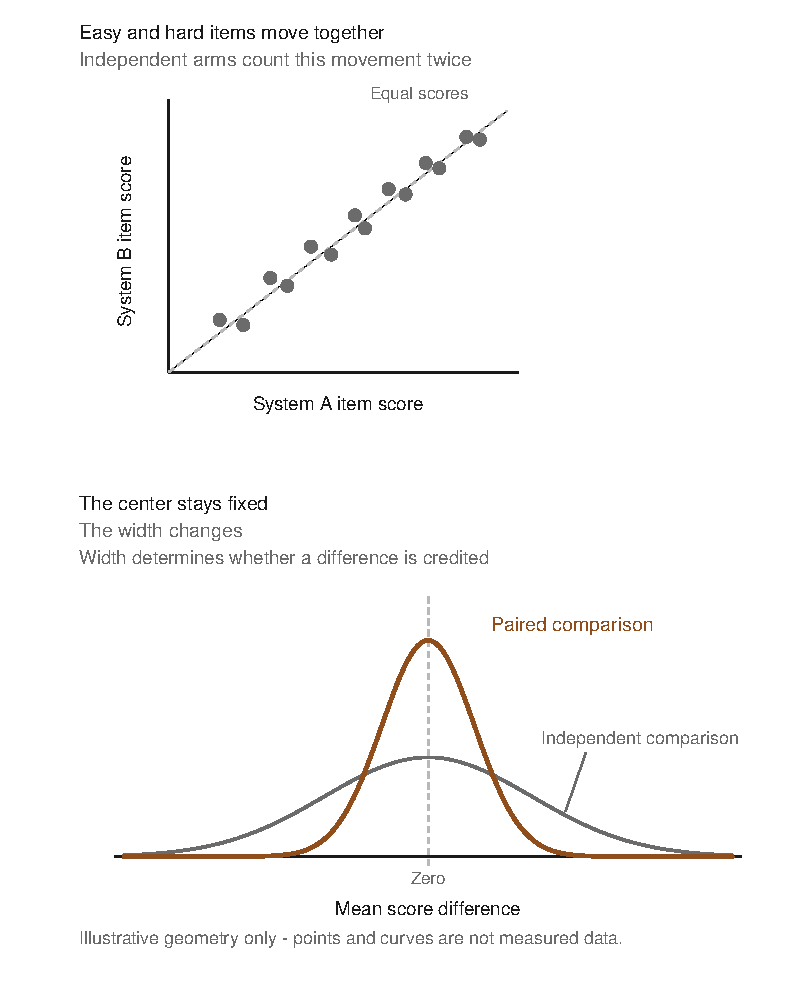
\includegraphics[keepaspectratio,alt={Illustrative, unmeasured geometry shows item scores for systems A and B rising together, while paired and independent mean-difference distributions share zero but pairing produces narrower uncertainty.}]{figures/ch01-paired-comparison.pdf}}
\caption{Illustrative, unmeasured geometry shows item scores for systems A and B rising together, while paired and independent mean-difference distributions share zero but pairing produces narrower uncertainty.}
\end{figure}

Item-level subtraction removes shared task difficulty, so the remaining variation better represents system disagreement. Positive covariance narrows uncertainty without changing the mean difference.

The interval around the mean difference is obtained by multiplying its standard error by an appropriate critical value. The choice of critical value and the validity of the approximation depend on the statistical procedure and the observed score distribution.

The data record must preserve the pairing. For every task, I retain the task identity, both system scores, the nuisance-source assignments, and the run identity. I report the mean paired difference, its standard error, an interval around that mean, and the correlation between the systems' item-level scores. Once the per-item relationship has been discarded, two headline means are not enough to reconstruct any of these quantities.

Pairing also improves diagnosis. The same average difference can arise from small gains across most tasks, a few large reversals, or a trade in which each system solves a different subset. Those patterns have different engineering implications. Item-level records reveal which tasks changed and whether the overall result depends on a small number of discordant cases.

The validity of the pairing depends on experimental identity, not matching task labels. Both systems must receive the same task state under the same execution and scoring apparatus. Repository revision, dependency state, tool permissions, time limits, and scoring logic are all part of the experimental unit. If any of them differ between the two arms, the subtraction no longer removes shared task difficulty because the systems did not receive the same item.

An adversarial review of one of my own experiment designs found this exact defect. One arm transformed the repository before presenting it to the system, while the other operated on the original repository. The task label remained the same, but the executable state did not. I therefore treated the planned pairing as invalid. A shared label does not establish that two experimental units are equivalent.

Published aggregate scores create a simpler boundary. If I did not run the other system on the same item instances, I do not have paired observations. The aggregate results can still be compared descriptively, but their item-level covariance cannot be recovered from the means. A valid paired analysis requires rerunning both systems on the same items.

Repeated attempts introduce the same identity requirement. Attempt one from system A pairs with attempt one from system B only when the attempts share randomized conditions by construction. Selecting pairs after inspecting the outcomes biases the comparison. Seeds, task order, data order, and other nuisance assignments must therefore be matched before results are visible and recorded with every pair.

The statistical procedure must also match the mathematical form of the outcome. When the reported score is the arithmetic mean of per-item numerical contributions, and the distribution of paired differences is reasonably compatible with a normal approximation, a paired t-test can test the mean difference and support a corresponding power analysis. That approximation should not be assumed automatically for small, discrete, skewed, or highly irregular samples.

Composite metrics require different treatment. An F-score is a nonlinear function of aggregate counts. There is generally no set of independent per-item F-scores whose arithmetic mean equals the corpus-level F-score. Corpus-level BLEU has a similar aggregation problem, and some forms of ROUGE may also depend on nonlinear or corpus-level aggregation. Applying a t-test to invented per-item metric contributions can produce a familiar p-value without satisfying the mathematical assumptions that give the test meaning.

A paired bootstrap preserves the relationship between the systems by resampling items as pairs and recomputing the full metric on each resampled dataset. A paired permutation test instead exchanges system labels within each observed pair under the null hypothesis. Neither requires the same normal approximation as a parametric t-test. Both still depend on choosing the correct resampling unit and having a sufficiently representative sample. The small-sample bootstrap failure described earlier occurred when the resampling unit was only a handful of runs.

Agent evaluations introduce outcomes that standard benchmark guidance does not fully resolve. Cost-weighted success combines task outcome with resource use. A pass or fail assigned by an imperfect grader includes uncertainty from the grading process. Neither outcome inherits a valid test merely because its final value lies between zero and one. The sampling unit, dependence structure, and aggregation rule must be specified before choosing the analysis.

The table below gives directional guidance. The recommendations for language-generation metrics come from the broader methodological guidance of Dror and Reichart (\href{https://arxiv.org/abs/1809.01448}{2018}) rather than from controlled comparisons of agent evaluations. The binary row applies \textbf{McNemar's test}, introduced by McNemar (\href{https://doi.org/10.1007/BF02295996}{1947}), the standard test for paired pass or fail outcomes. It analyzes the discordant pairs in which one system passes and the other fails. The table is a starting point, not a substitute for deriving the metric's actual sampling structure.

\begin{longtable}[]{@{}
  >{\raggedright\arraybackslash}p{(\linewidth - 4\tabcolsep) * \real{0.3333}}
  >{\raggedright\arraybackslash}p{(\linewidth - 4\tabcolsep) * \real{0.3333}}
  >{\raggedright\arraybackslash}p{(\linewidth - 4\tabcolsep) * \real{0.3333}}@{}}
\toprule\noalign{}
\begin{minipage}[b]{\linewidth}\raggedright
Outcome structure
\end{minipage} & \begin{minipage}[b]{\linewidth}\raggedright
Comparison to analyze
\end{minipage} & \begin{minipage}[b]{\linewidth}\raggedright
Test guidance
\end{minipage} \\
\midrule\noalign{}
\endhead
\bottomrule\noalign{}
\endlastfoot
Per-item numerical scores whose paired differences plausibly satisfy a normal approximation & Mean of the paired item differences & Paired t-test \\
Metrics computed nonlinearly from aggregate counts, including corpus-level F-score and BLEU & Full metric recomputed on resampled or relabeled item pairs & Paired bootstrap or paired permutation test \\
Pass or fail outcomes on the same items & Discordant pairs in which only one system passes & McNemar's test \\
\end{longtable}

A later chapter on retrieval freshness uses McNemar's test for this reason. Both systems receive the same items, and each item produces a pass or fail outcome.

The companion catalog covers designs that this basic framework does not. Clustered items require correlation-aware standard errors. Estimating pass@(k) from repeated attempts requires the appropriate combinatorial estimator. Claims spanning many tasks or metrics require multiplicity correction. Ranking several systems rather than comparing two requires paired-comparison ranking models with uncertainty intervals.

The catalog also covers profiling benchmark noise before making decisions, declaring the decoding configuration, aggregating scarce repetitions with interquartile means and resampled intervals, reducing an evaluation around a specific decision, using precommitted confirmatory designs, and measuring sensitivity across prompt variants. Each addresses a narrower problem than the core decisions developed in this chapter.

\section{Before drawing a conclusion from a difference}\label{before-drawing-a-conclusion-from-a-difference}

I define the engineering threshold before running the expensive suite. The threshold is the smallest change that would alter the engineering decision, not the smallest change a statistical test might detect.

Pilot variance then determines the required numbers of tasks and repeated runs. I add margin because the pilot estimate is itself uncertain, and the design record states the smallest difference the planned experiment can reliably resolve. When the available budget cannot resolve a difference large enough to matter, I narrow the claim or withhold the verdict before spending the calls.

Three independent repeats per configuration are my minimum. Three may still produce an unstable variance estimate, but they prevent one unusually favorable or unfavorable run from determining the result. I pair nuisance conditions across systems wherever possible and run both systems against identical item states. Each retained row records the item identity, the outcomes from both systems, the repeat identity, and the assigned random conditions.

The analysis begins with per-item differences. For continuous outcomes, I report the mean paired difference, its standard error, the correlation between the two systems' scores, and a confidence interval for the mean difference.

Binary pass-or-fail outcomes require the discordant pairs and an appropriate paired test. Nonlinear composite metrics require resampling or permutation of intact pairs. Matching task names do not create a paired design when the repository state, inputs, or execution path differs.

\Needspace{5\baselineskip}

Repeated trials remain interpretable only while the apparatus is pinned:

\begin{itemize}
\tightlist
\item
  model version;
\item
  decoding settings;
\item
  exact prompts;
\item
  task and repository revision;
\item
  tool definitions and permissions;
\item
  harness version; and
\item
  evaluator version.
\end{itemize}

When a provider exposes no stable model version, I record the evaluation window and treat later reruns as potentially affected by model drift.

The observed difference belongs beside the complete run distribution and the engineering threshold written before execution. I do not credit a difference that remains smaller than the measured variation. I return no verdict when the experiment lacked the power to resolve the difference that would have changed the decision.

\section*{Sources and evidence}

The evidence grouping on each entry below comes from its catalog record. Author-system cases in this chapter are narrative illustration and are not part of the evidence base.

\textbf{Never report a single run}

\begin{itemize}
\tightlist
\item
  Strong evidence: Ouyang, Zhang, Harman \& Wang (2023). An Empirical Study of the Non-determinism of ChatGPT in Code Generation. arXiv:2308.02828. Nominally identical requests, different programs and outcomes.
\item
  Strong evidence: Bjarnason, Silva \& Monperrus (2026). On Randomness in Agentic Evals. arXiv:2602.07150. The 60,000-trajectory result: 2.2 to 6.0 pp single-run spread, SD above 1.5 pp at temperature 0, early-token divergence.
\item
  Strong evidence: Reimers \& Gurevych (2018). Why Comparing Single Performance Scores Does Not Allow to Draw Conclusions About Machine Learning Approaches. arXiv:1803.09578. The 26\% result.
\item
  Strong evidence: Bouthillier et al.~(2021). Accounting for Variance in Machine Learning Benchmarks. MLSys 2021. arXiv:2103.03098. The \textasciitilde51x result and the fixed-seed critique.
\item
  Strong evidence: Henderson et al.~(2017). Deep Reinforcement Learning that Matters. AAAI 2018. arXiv:1709.06560. Five-seed splits and unreported researcher degrees of freedom.
\item
  Strong evidence: Dodge et al.~(2020). Fine-Tuning Pretrained Language Models: Weight Initializations, Data Orders, and Early Stopping. arXiv:2002.06305. The 2,100-trial seed result, scoped to small-data fine-tuning of pretrained encoders.
\item
  Prompt-variance finding: incorporated into this chapter's first developed practice, with its full evidence recorded in the companion catalog. Strong evidence: Sclar et al.~(2023), FormatSpread, arXiv:2310.11324; Mizrahi et al.~(2024), TACL, arXiv:2401.00595; and Salinas and Morstatter (2024), arXiv:2401.03729.
\end{itemize}

\textbf{Analyze statistical power before running}

\begin{itemize}
\tightlist
\item
  Strong evidence: Miller (2024). Adding Error Bars to Evals. arXiv:2411.00640 (Anthropic). The 13.2\% to 7.5\% minimum-detectable-effect example and the response-count lever.
\item
  Strong evidence: Card et al.~(2020). With Little Power Comes Great Responsibility. EMNLP 2020. arXiv:2010.06595. GLUE underpowering and effect-size exaggeration.
\item
  Strong evidence: Colas, Sigaud \& Oudeyer (2018). How Many Random Seeds? arXiv:1806.08295. The pilot floor, the bootstrap false-positive rate at small N, the DDPG case, and the preference for Welch's t-test.
\end{itemize}

\textbf{Use paired tests matched to the metric}

\begin{itemize}
\tightlist
\item
  Strong evidence: Miller (2024). Adding Error Bars to Evals. arXiv:2411.00640. Paired per-item differences with paired standard error and score correlation.
\item
  Directional evidence: Dror \& Reichart (2018). Appendix, Recommended Statistical Significance Tests for NLP Tasks. arXiv:1809.01448. The per-metric test selection; directional, so the table is guidance, not a measured result.
\item
  Foundational method: McNemar, Q. (1947). Psychometrika 12(2), 153-157. DOI: 10.1007/BF02295996. The paired pass/fail test used in the binary-outcome row.
\end{itemize}

\textbf{Author-system illustration cited inline}

\begin{itemize}
\tightlist
\item
  Not an evidence item: CodeProbe, the author's task-mining evaluation tool, \href{https://github.com/sjarmak/codeprobe}{public repository}. Named inline for the task-family run and rerun described in the opening, which are narrative illustration.
\end{itemize}


\chapter{Baselines, ablations, and cost-accuracy tradeoffs}
\label{ch02-baselines-ablations-cost-accuracy}
In one end-to-end run of CodeProbe (\href{https://github.com/sjarmak/codeprobe}{public repository}), the plain baseline came out ahead of the tool-augmented arm on both score and score per dollar. The configuration with the retrieval machinery in it lost to the configuration with none. That outcome was visible only because the run included a baseline at all. Reported alone, the tool arm's score would have had nothing to be read against, and a reader could have credited the retrieval machinery with whatever the number implied.

Published comparisons frequently omit the inexpensive arm. Kapoor et al.~(\href{https://arxiv.org/abs/2407.01502}{2024}) re-evaluated published agent architectures and found that on HumanEval, retrying the model could match more elaborate architectures at a fraction of their inference cost. When they optimized cost and accuracy jointly, they reduced cost without giving up accuracy.

Those results do not establish the same conclusion for repository-scale engineering. The re-evaluation is directional, and its coding evidence comes from a function-level benchmark. The comparison design transfers even when the finding does not. The inexpensive arm belongs in the experiment, and cost belongs in the report.

That omission changes the claim. A system with memory, retrieval, tools, or multiple agents may score higher than a direct model call. The score alone cannot tell us whether the added machinery caused the gain, whether another model call would have produced the same gain, or whether the comparison spent more until it found more successful samples. Engineering selection requires two coordinates: what the system accomplishes and what it consumes.

The available evidence supports comparison design rather than a universal cost threshold or recommended architecture. The chapter therefore develops controls that readers can run on their own workloads.

An elaborate system is worth keeping only when both comparisons support it. Its components must contribute something that remains when the rest of the experiment is held fixed, and the full configuration must beat the simple alternatives at a cost the operator is willing to pay. These are separate tests. Component removal addresses causal attribution. Direct-call and retry baselines address engineering value.

\hypertarget{remove-the-component-and-rerun-the-evaluation}{%
\section{Remove the component and rerun the evaluation}\label{remove-the-component-and-rerun-the-evaluation}}

An \textbf{ablation} removes one component and reruns the evaluation with the rest of the system and procedure held fixed. If a memory-enabled agent outperforms an agent without memory, the missing-memory arm estimates what the memory system contributed. If the comparison changes the model, prompt, task subset, token budget, harness version, or scoring procedure at the same time, the subtraction no longer isolates memory. It measures an unspecified bundle of changes. Without the missing-component arm, base-model capability and item difficulty remain plausible explanations for the observed score.

The component controls recur in two source corpora. SkillEvolBench, from Lei et al.~(\href{https://arxiv.org/abs/2605.24117}{2026}), reports no-skill and raw-trajectory controls for agent memory. CoIR, from Li et al.~(\href{https://arxiv.org/abs/2407.02883}{2024}), supplies the task and metric substrate for code retrieval, while the no-tool control comes from the associated evaluation-design synthesis. These sources support narrower measurements in their own settings; neither tests the complete repository-scale prescription developed here. Their convergence motivates the protocol, while the generalized recommendation remains directional.

Memory requires at least three arms. The first is the proposed memory system. The second is the no-skill control, which removes the written memory entirely. The third reuses the raw trajectory from prior work without asking a writer to consolidate it into a skill or memory record. The no-skill arm tests whether prior experience helps at all. The raw-trajectory arm tests whether the consolidation mechanism adds anything beyond retaining the original evidence.

Those two questions are easy to collapse into one. Suppose an agent that receives a distilled lesson solves more tasks than an agent starting from an empty context. The gain could come from the lesson, but it could also come from any useful tokens copied out of the earlier attempt. Raw-trajectory reuse makes that alternative visible. If the raw trace matches the distilled record, the experiment has shown that prior information helps, but it has not shown that the writer extracted a better representation.

The comparison also needs matched opportunities to retrieve. A memory arm evaluated on tasks for which a relevant record exists cannot be compared directly against a no-memory arm scored across a broader or harder task set. The primary comparison should be restricted to a coverage-matched subset, that is, the tasks for which the memory or retrieval system had a genuine opportunity to return relevant material. The full-set result should be reported separately, because coverage is itself an operational property. Unequal coverage should not be read as a difference in answer quality.

Retrieval and tool evaluations need a corresponding no-tool arm. Tool availability is an experimental variable and should be recorded with the rest of the arm configuration. The control gets the same base model, instructions, stopping conditions, and task instances, with access to the tool removed. If the treatment also receives a different system prompt, a larger context budget, or extra retries, those changes belong in additional arms or in a sweep that varies them one at a time.

One-factor sweeps matter because agent components interact. Retrieval can change context length. Context length can change model behavior. Tool schemas consume tokens before the agent begins the task. A different endpoint can expose a different tool set. A single comparison between `agent' and `baseline' assigns the combined effect to whichever feature appears in the label. Factorial experiments can estimate interactions when the evaluation budget supports them, but a sequence of one-factor comparisons is usually enough to find the first unsupported attribution.

An ablation result is conditional on the configuration in which the removal occurred. If retrieval helps only when a summarizer compresses its output, removing retrieval from the full system estimates retrieval's contribution with that summarizer present. The result does not show whether retrieval would help without summarization, or whether summarization would help without retrieval. Those questions require the corresponding component combinations as separate arms.

Skills and multi-agent structures need the same discipline, but their removal needs a more precise intervention. Deleting a skill while also shortening the prompt changes both procedural guidance and context length. Replacing several agents with one while reducing the call budget changes topology and sampling opportunity together. A useful control preserves the available information and budget wherever the design permits and removes only the coordination or representation being credited. When that preservation is impossible, an intermediate arm lets the comparison separate fewer model calls from a different arrangement of those calls.

Tank and Nama (\href{https://arxiv.org/abs/2607.22520}{2026}) compared agents with and without procedural skills across nearly 6,000 runs on two office-automation benchmarks and three model-harness stacks. The best-performing skills won primarily by causing fewer regressions, a distinction concealed by net task-success change. The study strongly supports decomposing a skill intervention into gains, regressions, and residual failures in those settings; transfer to coding-agent skill libraries remains directional.

The paired design from Chapter 1 belongs here. Each arm runs on the same tasks, task ordering and other sources of randomness are matched across arms wherever the execution system permits it, and the outcomes are analyzed as pairs. Otherwise, item difficulty can dominate the component effect. A retrieval arm that happens to receive more questions answerable by lexical lookup may appear superior even when the tool adds nothing on matched items.

Target size is a second confound of the same kind. A tool may look better when its index contains a narrow, curated collection and worse when it searches a large repository with many plausible distractors. Query coverage, corpus size, and retrieval depth should therefore be recorded with the configuration. If target size changes between arms, the experiment measures both the target and the retrieval algorithm.

In two studies from my own team, we asked the same practical question: does a retrieval tool help an agent? The positive-sign study was a paired comparison across many repositories, in which the tool arm came out slightly ahead. The negative-sign study was the CodeProbe run described at the start of this chapter, in which the plain baseline came out ahead. The two used different task curation and different enforcement of which arm had to use the capability under test. That experience is narrative illustration rather than independent evidence for the control method, but it exposed the mechanism. The apparatus decided which work entered the evaluation and whether the agent had to use the capability supposedly under test. The label on the treatment arm therefore did not identify a stable intervention.

Arm separation should be established at the task level through observed usage. A task cannot estimate a tool effect when the treatment completes it without touching the tool. Such a task may remain useful for measuring the agent's overall capability, but it contributes no information to the comparison of tool access.

In my own enterprise-scale benchmark, one candidate task ran for 41 turns without a single call to the tool under test. By every static check we had, it was a perfect task, and for the tool comparison it was useless. We removed it from the tool-effect comparison because both arms had effectively received the same treatment. Candidate tasks are hypotheses about discrimination, and a pilot run has to show that they actually separate the arms.

This gate should be empirical. For every candidate task, record whether the treatment invoked the component, whether the control could reach it through another path, and whether both arms received equivalent task information. A binary `tool enabled' field is inadequate when the agent may ignore the tool. Usage counts, arguments, returned bytes or tokens, and the point in the trajectory where the result entered context make the intervention observable.

The exclusion rule needs the same protection as any other post-hoc filter. Removal should be keyed to observed component usage and declared before the outcomes are inspected. Dropping tasks after seeing which arm won selects on the result, and it converts a usage gate into a mechanism for improving the reported effect.

Usage does not establish usefulness, but absence establishes non-use. If the treatment calls a retriever and then ignores its output, the task may still show a cost effect or an interference effect. If it never calls the retriever, its outcome cannot support a claim about retrieved information improving correctness.

The strongest boundary concerns information flow into the component. Evaluation labels and gold answers must stay out of any memory writer. A writer that sees the correct answer can encode it directly, encode a near paraphrase, or preserve features that make later retrieval trivial. Freezing the memory after that write does not repair the experiment, because the evaluated artifact already contains the target.

The same rule applies to the scoring target. A `right answer' generated with the tool or mechanism under evaluation cannot then be used to grade that mechanism by agreement with its own output. A retrieval system compared against answers assembled from the same retrieval system has been graded against its own oracle, the reference an evaluation scores candidate answers against. A target capable of disagreeing with the system requires independent human verification, or sources outside the evaluated path. Public benchmarks carry a related problem, because models have often already seen those tasks during training, an inflation channel Chapter 3 measures.

An ablation cannot remove every threat to inference, and it does not show that a useful component will remain useful under another workload. It answers a narrower question: under the evaluated task distribution and the fixed surrounding system, did removing this component change the measured outcomes? This question is narrow enough to test and strong enough to prevent a common attribution error.

The completed record should make the subtraction reproducible. Name the component removed, list every configuration field that remained fixed, identify the coverage-matched task subset, report component usage per task, and preserve the paired results. When multiple factors changed, describe the arm as a bundle and resist assigning its effect to one member of that bundle.

\hypertarget{select-on-accuracy-and-cost-together}{%
\section{Select on accuracy and cost together}\label{select-on-accuracy-and-cost-together}}

The support for this entry is one directional re-evaluation study and no strong evidence item. Kapoor et al.~(2024) covered a small set of benchmark families, including function-level coding, multi-hop question answering, and web-agent tasks. They did not establish the same result for repository-scale software work. Their contribution here is a comparison design that can be applied beyond those tasks. Evaluate the elaborate system against direct model calls and retries, then place accuracy and inference cost in the same result.

Additional model calls can raise the pass rate without any change to the architecture. If one attempt has probability \(p\) of passing and two attempts are independent, the probability that at least one passes is \(1-(1-p)^2\). The expression illustrates the effect under independence. It does not estimate real agent behavior, in which attempts are correlated. Correlation changes the size of the gain, but a system allowed to sample, revise, or delegate more often still has more opportunities to produce a passing output.

An accuracy-only ranking conceals those opportunities. It may rank a five-call scaffold above a direct call without showing that the improvement came from four additional samples. It may also compare one architecture with a retry loop against another configured to stop after its first answer. The ranking then credits budget and stopping policy under the name of architecture.

Use at least three initial arms. The direct-call arm sends the task to the base model with the minimum production-valid prompt and no scaffold. The retry-once arm makes one additional model attempt after a defined failure signal. The candidate arm runs the proposed architecture with its intended tools, memory, or delegation.

The failure signal in the retry arm must be available to the deployed system. Unit tests, a compiler error, or a schema validator can supply one. A hidden benchmark answer cannot. If the experiment retries only because the evaluator knows the first answer is wrong, that arm should be labeled oracle-assisted, because it otherwise understates the operational cost of deciding when to retry.

Model version, task set, and scoring target stay fixed across the three arms. Match any shared context required to attempt the task, but do not give the direct call internal traces that exist only because the scaffold ran. The inexpensive alternative has to be built credibly, since a deliberately crippled direct call provides no useful control. Record the stopping condition for every arm, because `one run' can mean one model response, one agent trajectory, or a tree of dozens of calls.

Cost accounting begins at the task boundary. Count all input and output tokens consumed after the task enters the system, including calls made by planners, delegates, critics, summarizers, and retries. When a provider bills cached input differently, preserve cache-read and cache-write quantities rather than folding them into an undocumented token total. Failed calls, timeouts that incur usage, and discarded branches are part of the cost of the configuration that created them.

Report token quantities even when the organization buys capacity rather than paying per request. Tokens remain a portable description of inference demand, while dollars depend on contract terms, provider prices, model aliases, and date. Convert the token ledger to money with a named pricing basis and a snapshot date. A dollar figure without that snapshot becomes uninterpretable after prices change.

Latency belongs beside this record when users wait for the answer or when workers occupy scarce execution slots. Latency and inference cost are not interchangeable quantities. Two arms can consume the same tokens while one serializes its calls and the other runs them concurrently. The parallel arm may reduce wall-clock time while raising peak capacity requirements. Cost, performance, and scheduling pressure therefore remain separate operational properties.

Plot each configuration by accuracy and cost. A configuration is Pareto-dominated when another configuration is at least as accurate and no more expensive, with a strict advantage on at least one axis. Dominated points drop out of consideration unless they supply some separately measured property the two-axis plot omits. The remaining points form the Pareto frontier. Moving along it trades accuracy for cost in one direction and cost for accuracy in the other.

The points on the plot should be configurations. Architecture names are too coarse, because model choice, retry limit, retrieval depth, and context budget all change both coordinates. A frontier built from configurations is usable for routing. Inexpensive settings may serve routine tasks, while costly settings are reserved for cases in which their measured gain justifies the added inference.

This rule is stronger than ranking by score per dollar alone. A ratio can favor a configuration that is cheap but below the minimum acceptable accuracy, or hide how much accuracy the additional spending returns at the high end of the curve. The frontier preserves the actual coordinates. Deployment constraints apply afterward: a minimum pass rate, a maximum per-task cost, or a latency ceiling measured for the workload.

\begin{figure}[htbp]
\centering
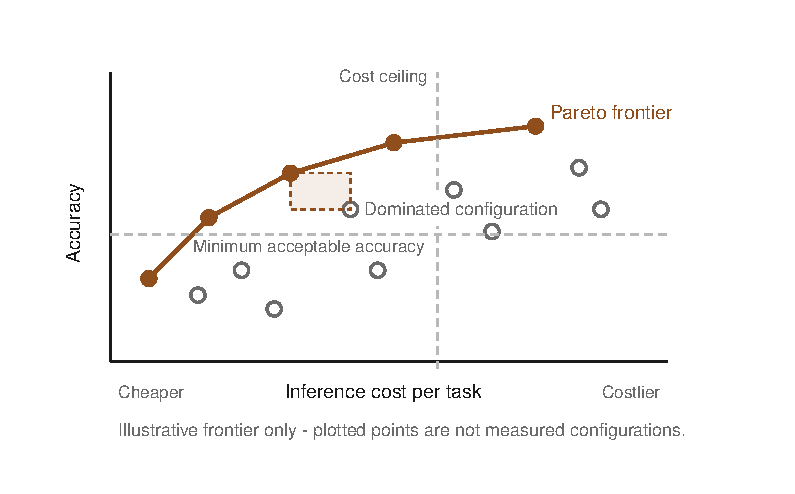
\includegraphics{figures/ch02-cost-accuracy-frontier.pdf}
\caption{Schematic of a cost-accuracy frontier, dominated configurations, and minimum-accuracy and cost-ceiling feasibility constraints.}
\end{figure}

Dominating configurations remove weaker alternatives unless an omitted property is measured separately. Deployment constraints then narrow the frontier.

The paired analysis from Chapter 1 keeps the frontier from acquiring false precision. Cost and accuracy estimates have uncertainty, and two nearby configurations may be indistinguishable at the available sample size. A single run also yields one realization of aggregate cost, which inherits the run-to-run variation that Chapter 1 describes for scores. The paired comparison runs on the per-task costs inside that run rather than on the aggregate. Preserve per-task cost as well as per-task correctness, so that bootstrap intervals can be computed for both axes and for the paired differences. A point should not be called cheaper or more accurate when the interval around that comparison does not support the ordering.

The retry arm needs the same accounting discipline as the candidate. If only some first attempts fail, report how often the second call fired, how much it cost when it fired, and whether it fixed the task. That record exposes the marginal value of the retry policy. A low-cost retry that recovers a meaningful subset of failures may dominate a planner with multiple unconditional calls, while a retry that repeats the same error adds cost without moving accuracy.

In CodeProbe, I report score per dollar alongside score and rank configurations by pass rate, cost, tokens, and latency. The end-to-end run in which the plain baseline led the tool-augmented arm on both axes came out of that report. It does not establish a general result about tools. Reporting both axes made the engineering decision visible without turning a small score difference into a claim about architecture.

Accuracy without a cost constraint still answers a legitimate research question. A model developer may want to know the highest capability reachable under extensive sampling, regardless of whether that procedure is economical in production. That is a capability probe. Selecting a system to operate under a budget is a different decision, and the result should state which decision the experiment was designed to support.

Architecture development introduces another source of optimism. An iteration \textbf{holdout} reserves a set of tasks that scaffold developers never use while choosing prompts, tools, routing rules, retry policies, or other configuration. Repeated iteration against a fixed evaluation set turns that set into training data for the scaffold, even when the model weights never change. Developers learn which changes improve the score, keep those changes, and discard the rest.

Create the iteration holdout before tuning begins. Use the remaining development tasks to debug the harness, compare early configurations, and decide what to carry forward. Open the iteration holdout only at a declared decision point, run the selected configurations, and do not use its task-level failures to continue tuning the same selection. If development resumes from those failures, the set has joined development and a new iteration holdout is needed.

The iteration holdout also needs protection from indirect tuning. A developer who reads its repository names, failure categories, or aggregate subgroup scores can adapt the scaffold to those features without inspecting the exact prompts. Access controls and an evaluation service that returns only the predeclared result can preserve the boundary better than a file accompanied by a policy. Record every opening, because repeated `final' checks use up the separation.

The cost of this discipline is fewer tasks for routine iteration. On small evaluations, that can reduce power enough to leave the final comparison inconclusive. The remedy is not to recycle the iteration holdout during development. Acquire more representative tasks, reduce the number of configurations carried into the final comparison, or accept a wider confidence interval. The boundary protects the interpretation of the result, but it does not add information the sample does not contain.

Search budget belongs in the accounting as well. If one architecture received hundreds of prompt and scaffold trials while the baseline received a single default configuration, the final inference-cost plot omits much of the effort spent finding the winner. Development cost and serving cost answer different questions. They should therefore be reported separately. At minimum, preserve the number of configurations tried, the selection rule, and the compute spent before the iteration holdout evaluation.

The companion catalog carries six related procedures. They cover expected best performance by tuning budget, repeated-sampling budgets based on coverage and verifier error, frozen-memory evaluation, a pinned scoring target, human-verified synthesis of evaluation instances, and baseline gates against random selection. Each refines a particular part of the experiment. None replaces the direct-call, retry, ablation, cost, and iteration-holdout controls developed here.

\hypertarget{build-the-next-comparison}{%
\section{Build the next comparison}\label{build-the-next-comparison}}

Start the next architecture comparison with the inexpensive arms. Run the base model directly, then run it with one retry under a failure signal the deployed system can observe. These controls establish how much of the candidate's accuracy another sample produces on its own, before a planner, memory writer, retriever, or second agent enters the design.

For each added component, create an arm without it and preserve every surrounding choice the design permits. When memory is the treatment, add raw-trajectory reuse so the experiment separates stored experience from the mechanism that rewrites it. When retrieval or tools are the treatment, add a no-tool arm, match task coverage, and record actual usage. Change one factor at a time unless the experiment is explicitly designed to estimate interactions.

Pilot the tasks before treating them as trials. Inspect each treatment trajectory and verify that the component entered the computation. A task the treatment never touches may measure general capability, cost, or incidental interference, but it decides nothing about the component's contribution. Remove it from that effect estimate under a rule declared in advance, or report it in a separate stratum.

Carry the per-task record from Chapter 1 into the cost analysis. For every arm, preserve correctness, input tokens, output tokens, priced cache quantities, call count, component usage, and wall-clock latency. Convert usage to dollars with a dated pricing snapshot. Plot accuracy against cost with confidence intervals, and prefer a configuration only when no cheaper configuration matches or exceeds its accuracy within the resolution of the evaluation.

Reserve the iteration holdout before the first scaffold change. Decide who can inspect it, when it can be opened, which aggregate results will be returned, and what event ends the comparison. Once developers have used its failures to revise the system, it has become development material. The boundary cannot be created retroactively around tasks the team has already learned to optimize.

\section*{Sources and evidence}

\textbf{Run ablation controls}

\begin{itemize}
\tightlist
\item
  Directional evidence: \emph{SkillEvolBench} (Lei et al.~2026, arXiv:2605.24117), through the agentic-memory source synthesis. The underlying study measures no-skill and raw-trajectory controls in its setting; coverage matching, one-factor sweeps, and the writer information-flow constraint are transfers within the broader protocol.
\item
  Directional evidence: evaluation-design material from the code-retrieval source corpus. CoIR (Li et al.~2024, arXiv:2407.02883) supplies code-retrieval tasks and metrics, but it does not test the no-tool baseline, tool-access control, or ground-truth-tautology checks recommended here.
\item
  Directional evidence: \emph{TIAP} (arXiv:2605.24060); no figure carried.
\item
  Directional evidence: \emph{MemConflict} (arXiv:2605.20926); no figure carried.
\item
  Strong evidence for the narrower transition analysis: Tank, D., and Nama, B. (2026), ``The Regression Tax: Decomposing Why Skills Help and Hurt LLM Agents,'' arXiv:2607.22520. Nearly 6,000 runs across two office-automation benchmarks and three model-harness stacks; transfer to coding-agent skill libraries is directional.
\end{itemize}

\textbf{Report cost-accuracy tradeoffs}

\begin{itemize}
\tightlist
\item
  Directional evidence: Kapoor, Stroebl, Siegel, Nadgir, and Narayanan (2024), \emph{AI Agents That Matter}, arXiv:2407.01502, a re-evaluation study.
\item
  Directional evidence: the iteration-holdout section rests on the same study, carried in the companion catalog as a separate record on holdout design split by generalization level.
\end{itemize}

\textbf{Author-system illustration cited inline}

\begin{itemize}
\tightlist
\item
  Not an evidence item: CodeProbe, the author's task-mining evaluation tool, \href{https://github.com/sjarmak/codeprobe}{public repository}. Named inline for the end-to-end run and the score-per-dollar reporting described above, both of which are narrative illustration.
\end{itemize}


\chapter{Benchmark contamination, oracle strength, and workload validity}
\label{ch03-contamination-oracle-workload-validity}
In February 2026, OpenAI (\href{https://openai.com/index/why-we-no-longer-evaluate-swe-bench-verified}{Feb 2026}) stopped reporting results on a benchmark subset it had helped create. In July 2026, it retracted its subsequent recommendation to use SWE-Bench Pro after an audit estimated that roughly 30 percent of its tasks were broken (\href{https://openai.com/index/separating-signal-from-noise-coding-evaluations/}{Jul 2026}). SWE-bench Verified had become one of the most cited measures of coding-agent performance. Its 500 tasks had survived screening by 93 paid professional developers, a process intended to remove ambiguous issues and defective tests. The sponsor later reported that 59.4 percent of 138 audited tasks had flawed tests: about 82 tasks, or 16.4 percent of the full 500-task subset. The same audit showed frontier models reproducing solution details verbatim when given only a task identifier.

Human screening had improved the original collection, but it could not control what happened after publication. \textbf{Contamination} is exposure to evaluation material before testing. Once tasks, issue discussions, reference patches, tests, and leaderboard results are public, they can enter training corpora, retrieval systems, fine-tuning sets, prompt libraries, and repeated development cycles. A clean review at release establishes nothing about those later paths.

The retirement also exposed a separate problem. Some tasks rejected functionally valid patches because the tests required an undocumented implementation detail or checked behavior absent from the issue. Other tests were too permissive and accepted patches that did not implement the requested behavior. Human review had missed both kinds of defect, because task quality is conditional on the candidates being graded. A test that looks reasonable in isolation can fail when it meets an implementation its authors did not anticipate.

You should treat any public score as the output of three coupled measurements. First, has the model already encountered the work? Second, can the test oracle refute an incorrect answer? Third, does the task distribution represent the work someone wants the model to do? The sponsor's reversal is the demonstration that reputation, curation effort, and a large annotator count answer none of these questions. Each question needs its own control.

\begin{verbatim}
public score
    ^
    |
    +-> has the model already encountered the work?
    |       -> matched control set
    |
    +-> can the test oracle refute an incorrect answer?
    |       -> adversarial test strengthening
    |       -> re-adjudication
    |
    +-> does the task distribution represent the work?
            -> tasks mined from the reader's own merged work

reputation + curation effort + large annotator count
    -> answer none of these questions
\end{verbatim}

\hypertarget{measure-the-public-private-gap}{%
\section{Measure the public-private gap}\label{measure-the-public-private-gap}}

The first control is a point-in-time audit that any evaluator can commission. A \textbf{matched control set} reproduces the public suite's relevant difficulty characteristics using tasks the benchmark never released. Running both sets under the same protocol produces a separate public-private gap for each model.

Prathifkumar et al.~(\href{https://arxiv.org/abs/2512.10218}{2025}) conducted an observational comparison and found roughly a threefold overall advantage and a sixfold file-localization advantage on SWE-bench Verified relative to their control tasks. The comparison covered popular open-source Python projects, but it did not establish that the individual issues were equally difficult. Unresolved differences in task difficulty therefore remain a plausible explanation for part of the observed gap.

This audit provides a point-in-time measurement. The post-cutoff pipeline in the next section provides a standing control, avoiding the need to reconstruct the comparison each time the public benchmark ages.

An evaluator usually cannot inspect a model's complete training history. Providers rarely publish full training corpora, and even a searchable disclosed corpus would omit later fine-tuning, generated training examples, and indirect exposure through task discussions or benchmark-driven development. Asking whether a model has seen a particular item creates an attribution problem without reliable ground truth. Asking how its performance changes on comparable unseen work produces an observable difference.

The audit requires two task sets that differ in public exposure while matching as closely as possible on the features that determine difficulty. For repository work, those features include programming language, repository scale, issue format, expected patch size, dependency burden, and the amount of localization required before editing. The model, harness, prompt, tool access, retry policy, and scoring procedure remain fixed across both sets.

When each public task has a defensible counterpart, the audit should use a paired design so the analysis can compare outcomes within each matched pair.

For a given model, the primary estimate is:

\begin{verbatim}
inflation_gap(model) =
    score(model, public_tasks) - score(model, matched_control_tasks)
\end{verbatim}

The gap estimates the combined effect of public exposure on the measured score. It cannot isolate a pure training-data effect. The estimate may include direct exposure to tasks or solutions, familiarity with repositories and issue conventions, and adaptation through repeated use of the public suite.

That final channel does not require any change to model weights. Each time developers evaluate an agent on a public suite, retain a change that raises its score, and discard one that lowers it, the development process adapts to the suite. The iteration holdout described in Chapter 2 protects a local development process from this form of selection. The matched comparison estimates the inflation that remains across all exposure channels together.

A single audit is also a single realization. The gap inherits the run-to-run variation described in Chapter 1, so both task sets require repeated runs before their difference can be interpreted as an estimate rather than one draw.

There are three practical ways to construct the comparison set. A \textbf{private mirror} reproduces the public suite's collection procedure using tasks that have never been released. A \textbf{newly collected set} samples recent work from the same task family. A \textbf{retroactive twin set} reconstructs tasks with the same measured properties, provided the model's training cutoff predates publication of the twins. Each supports a narrower claim than the phrase ``clean benchmark'' suggests.

A private mirror provides the strongest control over exposure, but it is expensive to construct. Repository tasks require reproducible code states, issue descriptions, reference changes, and tests that distinguish acceptable from unacceptable patches. The mirror loses its protection once it is released, distributed broadly to vendors, or used repeatedly during agent development. Access logs, handling rules, and usage history therefore become part of the measurement because the set's exposure status changes over time.

Newly collected tasks are less expensive when a team already has a stream of resolved work. Their recency makes prior exposure less likely, but it may also introduce a different mixture of repositories, framework generations, and issue types. A lower score may therefore reflect unfamiliarity, greater difficulty, or both.

Matching requires an explicit adequacy check. Similar averages are not enough. The evaluator should determine whether the feature distributions overlap, whether individual pairs are defensible in engineering terms, and whether the conclusion survives the removal of visibly poor matches.

Retroactive twins make the matching problem especially visible. Haimes et al.~(\href{https://arxiv.org/abs/2410.09247}{2024}) constructed twins for a public question-answering benchmark and required them to pass four statistical indistinguishability checks before comparison. Across 20 models, some public scores exceeded twin scores by as much as 16 percentage points. A substantial public-private gap can therefore remain even after formal matching checks are satisfied.

Those results do not establish a comparable gap for repository-scale coding. The twins were constructed and validated for question answering, and the method applies only when the model's training cutoff predates publication of the twin set. The 16-point result is the largest gap observed under that study's design. It is not a bound on coding benchmarks and should not be used as a correction factor for coding scores.

A controlled arithmetic study provides another boundary. Zhang et al.~(\href{https://arxiv.org/abs/2405.00332}{2024}) reconstructed a grade-school arithmetic benchmark as a private mirror and measured accuracy drops of up to eight percentage points. The model-level gap was also associated with the probability that a model would reproduce public items verbatim; the results section reports Spearman's rank correlation as \(\rho=0.36\) with \(p=0.03\).

Many frontier systems showed little overfitting, and every evaluated model generalized to the novel items. That variation is why the audit must be performed separately for each model. Exposure and score inflation are properties of a particular model-benchmark pair. Applying one average correction across models would erase the model-specific signal the audit is intended to measure.

The observational coding result is more directly relevant to software work but less controlled. Both sides used popular open-source Python projects, yet matching at that level does not establish equivalent issue difficulty. A model may localize files more easily in repositories it has encountered repeatedly, which is itself a meaningful familiarity effect. The observed performance difference may also include repository-specific complexity.

The reported threefold and sixfold gaps should therefore be treated as directional evidence, with the matching limitation attached whenever those figures are used.

The audit should produce a separate record for each model containing the public score, matched-control score, paired difference where pairing is justified, and uncertainty for each quantity. It should also document the task-matching procedure closely enough for another evaluator to challenge it. A single pooled gap is inadequate because models differ in both exposure and generalization. A corrected leaderboard is worse because it converts uncertain, model-specific estimates into false precision.

The decision depends on the size and stability of the measured gap. A small gap with a wide confidence interval means the audit lacked the resolution to establish much. A large gap that survives plausible rematching indicates that the public score is a poor estimate of that model's performance on comparable unseen tasks.

Neither result establishes how the model will perform on the reader's repositories. The audit answers a narrower question: whether public availability appears to change the measurement.

\hypertarget{keep-the-task-window-ahead-of-the-model}{%
\section{Keep the task window ahead of the model}\label{keep-the-task-window-ahead-of-the-model}}

A \textbf{temporal holdout} tags every task by publication time and evaluates a model only on work published after its stated training cutoff. This is the standing pipeline. The matched comparison in the previous section is the point-in-time audit, and a reader who adopts that audit alone has to keep commissioning new ones as the public set ages. The pipeline removes that repetition at a real cost. Longitudinal comparability weakens, because every time window contains different work.

The control removes the most direct path from a public task into pre-evaluation training. Suppose a model's stated cutoff is June 2025. An issue first published in August can enter its evaluation window, while an issue published in May cannot, even when both are assembled into the benchmark in September. The relevant date belongs to the underlying task material rather than to the benchmark's ingestion.

That distinction changes the data model for an evaluation suite. Each task needs provenance for its issue, repository state, tests, solution, and any discussion that reveals the solution. Each model needs a recorded cutoff and a policy for ambiguous or rolling cutoffs. Eligibility is then a function of both records:

\begin{verbatim}
eligible(task, model) =
    task.first_public_at > model.training_cutoff
\end{verbatim}

The inequality is the easy part. \texttt{first\_public\_at} may refer to an issue that was discussed in a public chat before it reached the tracker, a security fix disclosed after private coordination, or a commit mirrored across several hosts. A benchmark maintainer must choose which event counts and retain enough provenance to revisit that choice. Cutoff claims pose a similar problem, because providers may disclose a date without specifying whether later supervised tuning, tool traces, or retrieval indexes include newer material.

Eligibility is also a property of a task-model pair rather than of a task set. A collection labeled post-cutoff without naming the model it was checked against establishes nothing about eligibility.

Controlled evidence from continuously collected coding problems shows why the date split is still useful. Jain et al.~(\href{https://arxiv.org/abs/2403.07974}{2024}) tagged problems by release date and found that some model families lost substantial performance on problems published after their cutoffs. The same time-windowed scoring exposed overfitting to an older function-level suite, because models that scored well on it dropped on a fresh distribution. The discontinuity is stronger evidence than a memorization probe alone, because it connects temporal eligibility to the score being interpreted. It remains conditional on the accuracy of the disclosed cutoff and on the comparability of adjacent task windows.

Repository-scale live collections provide directional support. Zhang et al.~(\href{https://arxiv.org/abs/2505.23419}{2025}) rebuilt the issue-to-environment recipe continuously, with a reproducible environment built per task, and reported that the same systems scored well below their results on a frozen suite. Badertdinov et al.~(\href{https://arxiv.org/abs/2505.20411}{2025}) ran a continuous collection pipeline with decontaminated evaluation and hedged that some models' frozen-suite scores may be inflated by contamination. Adamenko et al.~(\href{https://arxiv.org/abs/2507.11059}{2025}) described a continuously updated pipeline that draws on roughly 10,000 potential tasks and passes a small fraction of them through automated gates into the released benchmark. These results show that live evaluation is operationally possible and that frozen and fresh distributions can disagree. They do not isolate direct training exposure from changes in repositories, issue difficulty, or curation.

A standing pipeline has four recurring jobs: gather new work, reconstruct a reproducible environment, reject invalid tasks, and publish results by time window. Failure in any stage can look like a model failure. A missing dependency lowers scores without establishing anything about capability. A permissive filter raises scores by admitting trivial tasks. A delayed ingestion process can place nominally new work behind a model's actual exposure. Freshness is therefore a property of the whole collection process.

Automated gates make continuous collection affordable, but they are less discriminating than expert review. A window of a few hundred accepted tasks also produces wider uncertainty than a large fixed suite, especially when results are split by language or task type. The temptation is to combine windows until the interval narrows. Combining them can cross a model cutoff or merge meaningfully different task distributions, which removes the temporal property that justified the pipeline.

The longitudinal trade is unavoidable. If Model A is evaluated in March and Model B in September, their eligible sets differ. If one fixed set is retained for both, it stops being post-cutoff for the later model. Rolling-window results should be the ones reported for current validity, and a fixed suite belongs beside them only when a trend line is necessary. The fixed series answers how systems change on one historical instrument. The rolling series answers how they perform on currently eligible work.

Comparability needs its own audit. A dynamic benchmark introduces generators, source selection, filters, environment builders, and a refresh cadence, and each of those can change the score independently of the model. Chen et al.~(\href{https://arxiv.org/abs/2502.17521}{2025}) surveyed the shift from static to dynamic evaluation, identified the absence of standardized criteria for judging a dynamic benchmark, and proposed design principles for building one. Their principles are prescriptive rather than tested at scale. Three inspection questions follow from them for a reader assessing someone else's live result: how the pipeline enforces cutoff hygiene, what quality control runs on regenerated tasks, and how comparability across snapshots is accounted for. The word `live' supplies no evidence about any of those mechanisms.

Temporal separation has two further limits. A model provider may have private prerelease access to material that becomes public later. The public timestamp can therefore follow actual exposure. Once a live window is released, later models can train on it and the window becomes historical. The pipeline preserves a moving boundary by continuing to collect tasks and applying eligibility per model. A benchmark does not stay clean permanently.

In one of my evaluation frameworks, a pre-cutoff and post-cutoff split is written into every result record, keyed to repository creation date and model cutoff, with a warning above a five-percentage-point gap. Repository creation date is a coarser field than the eligibility rule above requires, because a repository can be created years before the issue that becomes the task. This illustrates a methodology and supplies no evidence that the threshold detects exposure. The warning has fired only on replayed fixtures and never on live data. Retaining the split permits recomputation when better dates or cutoff information arrive, while a single aggregate would require reconstruction.

The companion catalog extends these two controls without turning them into one omnibus procedure. Its related entries cover memorization probes, semantic-overlap searches across paraphrases and translations, per-model and per-benchmark audits, and detector combinations chosen for a stated threat model. Other entries address anti-searchable task construction, protecting evaluation data at release, and attaching measured score benefit to a detector's finding. That last proposal has thin support. It remains a research direction and supplies no correction factor.

\hypertarget{make-passing-patches-harder-to-preserve}{%
\section{Make passing patches harder to preserve}\label{make-passing-patches-harder-to-preserve}}

A passing patch can fail to support the capability claim for three independent reasons, and they do not all fail in the same way. Training contamination means the model encountered evaluation material before the run. Solution leakage means the benchmark item included its answer during the run, in the issue text or in the comments. Those two can produce a correct patch while removing the grounds for attributing it to independent problem-solving. A weak oracle is the third defect, in which the tests cannot refute an incorrect patch, and only this one lets a wrong patch pass. The remedies are respectively temporal or access controls, removal of answer-bearing task material, and stronger tests.

All three failures can produce a successful-looking transcript. A model may reproduce a reference patch it saw during training, copy an answer supplied in the prompt, or find a shortcut that satisfies shallow assertions. The final test process records the same state in each case: pass. Transcript inspection and contamination probes cannot compensate for a test suite that accepts wrong behavior, and added tests cannot establish whether the model recalled the right behavior.

Shao et al.~(\href{https://arxiv.org/abs/2607.22368}{2026}) make this broader condition explicit as protocol validity: the intended capability must remain necessary for success under the evaluation protocol. Their HackDetect audit covered 2,385 traces across 15 agent benchmarks and found exposures or reward hacking in 67.0 percent of Frontier Science traces and 66.7 percent of AutoLab tasks; paired audits measured score inflation of 0.45 to 1.00 on their Mislead-gap scale. These are strong measurements for the audited protocols, not prevalence estimates for agent benchmarks as a whole.

I therefore treat a passing patch as a hypothesis about correctness. The test oracle is the ordinary continuous-integration mechanism that decides whether the candidate passes or fails. Its strength is the range of plausible wrong behavior it can reject. A suite is stronger when it checks more of the behavior implied by the task, especially behavior that superficially reasonable patches get wrong.

Function-level code generation provides a controlled example. Liu et al.~(\href{https://arxiv.org/abs/2305.01210}{2023}) expanded a widely used suite's tests by 80x with generated inputs and mutation-based cases. Across 26 models, the largest relative reductions in \(\mathrm{pass}@k\) ranged from roughly 19 to 29 percent across the reported values of \(k\), and model rankings changed. The models and generated programs were fixed; only the observations used to decide correctness changed. The original ranking had partly measured which wrong programs happened to fit sparse tests.

Repository-scale results show the same mechanism under more realistic state. Yu et al.~(\href{https://arxiv.org/abs/2506.09289}{2025}) augmented SWE-bench tests retroactively and found 36 under-tested tasks and 345 patches that had been labeled as passing incorrectly. Re-adjudication corrected 40.9 percent of entries on the smaller suite and 24.4 percent on the human-screened suite, changing 29 rankings. This was an audit of already reported results, so oracle weakness had propagated beyond individual tasks into system comparisons.

Task construction can fail before the oracle runs. Wang, Xu, and He (\href{https://arxiv.org/abs/2607.28587}{2026}) audited SWE-bench Verified and found PR-issue misalignment in 13.6 percent of instances across five patterns and eleven scenarios. Their PAIChecker reached up to 92.12 percent binary accuracy on SWE-Gym and 91.67 percent on SWE-bench Multilingual across four model backbones. The results strongly support the measured misalignment rate and detector accuracy on those collections; other SWE-bench-derived sets require their own audit.

The problem predates current coding models. Ye et al.~(\href{https://arxiv.org/abs/1909.13694}{2019}) generated random tests against a human reference patch and assessed 638 candidate patches from 14 repair systems. The added oracle improved automatic patch assessment by 190 percent over the prior methods used in that comparison. The historical context is useful because it locates the defect in test-based program repair itself. Generative models make candidate production faster and more varied, but shipped tests are not equivalent to a specification.

Adversarial strengthening begins from the candidate failures a benchmark should reject. Construct plausible patches that implement only the common case, hard-code a fixture, change an unrelated return value, suppress an exception, or satisfy the visible assertion while violating the issue's broader contract. Then retain the tests that kill those patches. Yu et al.~(\href{https://arxiv.org/abs/2603.00520}{2026}) built suites that way, rejected 19.71 percent of patches that had passed previously, and reported a top score falling from 78.80 percent to 62.20 percent.

Four audits test apparent benchmark success under stronger oracles. SWE-Bench+ covers one agent-model pair, so its percentages remain specific to that evaluation.

This process searches a different space from ordinary coverage expansion. Generated inputs explore more executions of a trusted implementation. Mutation-based cases perturb code to reveal assertions that fail to notice behavioral changes. Differential tests run the candidate and a trusted reference on the same inputs, then compare the results. Wrong-patch construction starts from foreseeable shortcuts and asks whether the suite detects them. A strong audit combines these approaches, because each makes a different assumption about where missing behavior resides.

The trusted reference is the central dependency. Random or generated tests need expected outputs, and differential testing needs behavior worth treating as ground truth. A human patch can contain unrelated changes or encode only one acceptable design. When the issue permits several implementations, exact agreement with that patch can reject valid alternatives. The evaluator must distinguish behavioral equivalence from textual or structural similarity, while accepting that some behavior remains underspecified.

Manual review addresses failures that generated tests are unlikely to expose. Aleithan et al.~(\href{https://arxiv.org/abs/2410.06992}{2024}) screened the apparent SWE-bench successes of one agent and model pair and found that 32.67 percent involved solution leakage and 31.08 percent passed weak tests. Removing those cases dropped the reported resolution rate from 12.47 percent to 3.97 percent. The scope is one pair, and the percentages do not estimate the prevalence for other agents or models. They show that leakage and oracle weakness can occupy a large share of one system's credited successes.

That study also clarifies why solution leakage belongs here. An issue may include the intended algorithm, a maintainer comment with the decisive condition, or a link to the merged fix. The model has legitimate access to that content during evaluation, so a training cutoff cannot remove it. If the deployment workload includes equally explicit issue discussions, retaining the material may be valid. If the benchmark claim concerns inferring fixes from ordinary bug reports, the leaked solution changes the task being measured.

In my own audit of an enterprise-scale benchmark, I scored a null agent that merely repeated each instruction against every gradeable task. Some verifiers awarded the echo credit. One gave full marks because its checker searched for vocabulary that appeared in the prompt itself. An agent with no capability at all is a cheap adversary, and it found real defects. The audit supplies no capability estimate, but it demonstrates a useful attack. Submit candidates that contain task language without task behavior, then inspect every nonzero grade.

Re-adjudication is the step that makes a strengthened oracle consequential. Run the stronger suite on stored patches from every system under comparison, including older submissions. Recompute \(\mathrm{pass}@k\), rankings, paired differences, and any reward or release gate derived from the old labels. That recomputation has to start from the stored per-attempt outcomes rather than from a rescaling of the published rate, because \(\mathrm{pass}@k\) is estimated from attempts.

Report the survival fraction, the number of tasks whose adjudication changed, and the uncertainty remaining after invalid tasks are removed. A suite that changes only one system's labels may expose a system-specific shortcut. Broad changes point toward a benchmark-level defect.

Additional tests provide one-sided evidence. They can disprove more candidates by finding counterexamples. A surviving patch has resisted the tests run so far, but it has not been certified correct for every valid input and environment. That boundary is tighter for repository tasks, because their behavior depends on configuration, dependency versions, persistent state, concurrency, and interactions outside the changed function.

Strengthening also has a coverage boundary. One of these efforts strengthened only about half of its benchmark instances. Its corrected rate remains an upper bound, because weak passes may persist in the untouched half and in behaviors the new tests still omit. Manual review is expensive, generation can reproduce assumptions embedded in the reference, and an adversarial patch set can miss shortcuts no one imagined.

The practical stopping rule follows the decision being made. For a research comparison, sample-based manual review and broad generated augmentation may bound the inflation well enough to qualify the claim. A release gate on the reader's own repository requires closer alignment with the actual acceptance criteria and failure costs. In both settings, the evaluator should publish how many old passes survived. Reporting only the strengthened score hides the size and the location of the correction.

\hypertarget{move-the-instrument-onto-your-work}{%
\section{Move the instrument onto your work}\label{move-the-instrument-onto-your-work}}

When a public ranking conflicts with sustained field behavior, the first question is whether the two measurements represent the same work. The evidence behind this practice is the thinnest in the chapter. It rests on one directional, practitioner-authored production benchmark and one anecdotal practitioner account, with no strong item standing behind it. The prescription asks the reader to build and measure on the relevant workload. It supplies no vendor score to adopt.

Construct validity asks whether an instrument measures the property named in the claim. Bean et al.~(\href{https://arxiv.org/abs/2511.04703}{2025}) used that question as the checklist for a systematic review of 445 benchmarks. A coding benchmark can measure repository issue resolution while offering weak evidence about migration work, security remediation, build repair, or long-running feature development. Passing tests establish performance on the sampled tasks under the specified harness. Generalizing that result to another workload requires a reason to believe the task distributions and operating conditions overlap.

Public repository suites usually select work that can be reconstructed from visible artifacts. This favors languages with reproducible environments, projects with mature tests, issues linked cleanly to merged changes, and tasks short enough to run economically. A production workload may contain private dependencies, sparse tests, organization-specific conventions, partial requirements, abandoned attempts, incident response, and changes whose value appears weeks later. The public suite can be carefully built and still omit the state transitions that dominate the deployment.

Construction should start with the work product and trace backward. For a coding assistant, candidate tasks include production prompts, accepted changes, review outcomes, and the tests associated with completed work. The evaluation record should preserve the repository state available at task start, the instruction as received, the permitted context and tools, and the evidence that caused the organization to accept the result. Other domains need their own decision sequence and artifacts. A general reasoning proxy omits that structure.

Jha et al.~(\href{https://arxiv.org/abs/2604.01527}{2026}) demonstrated one curation approach for a production-derived benchmark. They built tasks from sessions with their own coding assistant, classified the work, checked that tests were relevant to each task, and required stability across repeated runs. This is directional evidence from one vendor's environment. It shows that production traces can be converted into repeatable tasks. It does not establish that the resulting distribution represents another organization, or even every kind of work inside the source organization.

The anecdotal account identifies a transfer failure worth testing. Bytesfortruth (\href{https://www.reddit.com/r/compsci/comments/1rqcmu8/}{2026}), a lending-domain practitioner, reported that a model near the 90th percentile on a general-reasoning measure failed basic mortgage-underwriting tasks, and that rankings changed considerably on a domain-lifecycle evaluation. The account covers one team and reports no failure frequencies. It establishes one transfer failure and supplies no population rate for domain mismatch.

The task-sampling frame should follow the deployment claim. A tool meant to fix failing tests needs a distribution of actual failures, including the hard and unresolved ones. A tool meant to draft small maintenance changes needs accepted small changes plus representative rejections. Mixing those claims into one private score recreates the ambiguity of a general leaderboard under local ownership.

In my own work, I built CodeProbe (\href{https://github.com/sjarmak/codeprobe}{public repository}) to mine evaluation tasks from a repository's merged pull requests. It keeps the instruction separate from the recorded ground-truth commit and uses the test files touched by the original change as the verification command. That design turns completed work into replayable cases without exposing the recorded solution to the candidate. It is a methodology illustration and carries the same oracle caveat as any test-derived benchmark. The tests a merged change happened to touch are candidate historical checks, not a certification that the recorded solution was correct.

Merged history is a selective record. Language filters and minimum-file thresholds exclude some changes before sampling begins. Requiring touched tests favors well-instrumented code, while abandoned work and incidents may leave no merge to mine. The resulting set is closer to the repository's accepted work by construction, but its representativeness remains bounded by what the workflow recorded and what the miner can reconstruct.

Consent and data handling also constrain the instrument. Production prompts can contain customer data, credentials, internal incidents, or employee-authored material collected for a different purpose. Redaction may remove the context that made a task difficult. Broad access may create a new exposure path. A private evaluation program therefore needs explicit collection authority, access controls, retention rules, and a record of who has seen each task.

Long-horizon outcomes create a different measurement problem. A patch can pass today and produce maintenance cost later, and a generated migration can complete while leaving operational cleanup for another team. These labels arrive slowly and contain organizational noise. Pairing offline task results with later online outcomes helps test whether the local instrument predicts the field, though sparse failures make tail estimates unstable.

When public and local results disagree, the instrument whose construction supports the deployment claim is the better guide. That ordering is conditional. A small private set with weak tests can be less informative than a mature public suite. A small private set also inherits the resolution limits from Chapter 1, and with a few dozen tasks, differences smaller than its minimum detectable effect are not reliably distinguishable from noise. The local set earns priority by preserving relevant work and surviving repeated measurement. Privacy alone does not add validity.

A locally mined task set is also the raw material for the release instrument in Chapter 4, which curates a subset of these tasks into a golden set, replays it for each release, and attaches an executable gate.

The companion catalog carries the remaining validity checks. They include real temporal holdouts for agent benchmarks, pinned evaluation apparatus and published scored artifacts, ranking stress tests under perturbation, invalid-item purges, and audits of leaderboard submission protocols and questionable research practices. It also includes construct-validity checks, code-benchmark review against defect taxonomies, searches for an adequate benchmark before building one, and paired offline and online evaluation. The proposals on score-anchored contamination metrics, submission-protocol audits, and defect-taxonomy vetting have thin support and supply no evidence for any claim in this chapter.

\hypertarget{discount-the-next-public-number}{%
\section{Discount the next public number}\label{discount-the-next-public-number}}

The next time you encounter a public benchmark number, identify the answers to these 4 questions before using it.

\begin{enumerate}
\def\labelenumi{\arabic{enumi}.}
\tightlist
\item
  How old are the tasks relative to this model's training cutoff? Look for a public-versus-matched gap measured on this model. Do not substitute the leaderboard average or another model's audit.
\item
  How strong is the test oracle? Ask whether anyone augmented the tests, constructed adversarial wrong patches, or manually screened apparent successes. The useful result is the fraction of previous passes that survived.
\item
  Who produced the number, on which harness, with what task distribution? Compare the languages, prompt forms, repository structures, time horizons, context, and acceptance criteria against the work you need done.
\item
  What does the same protocol report on tasks mined from your team's merged work? Preserve the original instruction, pre-change state, acceptance evidence, and repeated-run uncertainty.
\end{enumerate}

These answers do not yield a universal correction formula. They turn one impressive-looking score into a bounded claim: performance by a named system, under a named apparatus, on work with a known exposure history, judged by tests with observed power to reject wrong patches. The local replay tests that claim on the work the system will actually be asked to do.

\section*{Sources and evidence}

\textbf{Opening scene}

\begin{itemize}
\tightlist
\item
  OpenAI, ``Why SWE-bench Verified no longer measures frontier coding capabilities,'' 2026-02-23, \url{https://openai.com/index/why-we-no-longer-evaluate-swe-bench-verified}. {[}Corroborating evidence{]}
\item
  OpenAI, ``Separating signal from noise in coding evaluations,'' 2026-07-08, \url{https://openai.com/index/separating-signal-from-noise-coding-evaluations/}. {[}Corroborating evidence{]}
\item
  SWE-bench Verified card: 500 instances, 93 professional screeners. {[}Benchmark record{]}
\end{itemize}

\textbf{Measure public-score inflation with matched controls}

\begin{itemize}
\tightlist
\item
  Prathifkumar, Saji Mathews \& Nagappan (2025), arXiv:2512.10218, Waterloo. {[}Directional evidence{]}
\item
  Zhang, H. et al.~(2024), GSM1k, arXiv:2405.00332, Scale AI. {[}Strong evidence{]}
\item
  Haimes, Wenner et al.~(2024), arXiv:2410.09247, Apart Research. {[}Strong evidence{]}
\item
  Corroboration: none on record.
\end{itemize}

\textbf{Evaluate on post-cutoff tasks}

\begin{itemize}
\tightlist
\item
  Jain et al.~(2024), arXiv:2403.07974, LiveCodeBench, ICLR 2025. {[}Strong evidence{]}
\item
  Zhang, L. et al.~(2025), SWE-bench Goes Live!, arXiv:2505.23419, Microsoft Research. {[}Directional evidence{]}
\item
  Adamenko et al.~(2025), arXiv:2507.11059, SWE-MERA. {[}Directional evidence{]}
\item
  Badertdinov et al.~(2025), arXiv:2505.20411, SWE-rebench, Nebius. {[}Directional evidence{]}
\item
  Chen, S. et al.~(2025), arXiv:2502.17521, static-to-dynamic benchmark survey. {[}Directional evidence{]}
\end{itemize}

\textbf{Strengthen test oracles before adjudication}

\begin{itemize}
\tightlist
\item
  Liu, Xia, Wang \& Zhang (2023), arXiv:2305.01210, HumanEval+ / EvalPlus, NeurIPS 2023. {[}Strong evidence{]}
\item
  Yu, S. et al.~(2025), arXiv:2506.09289, UTBoost. {[}Strong evidence{]}
\item
  Ye, Martinez \& Monperrus (2019), arXiv:1909.13694. {[}Strong evidence{]}
\item
  Aleithan et al.~(2024), arXiv:2410.06992, SWE-Bench+. {[}Directional evidence{]}
\item
  Yu, B. et al.~(2026), arXiv:2603.00520, SWE-ABS. {[}Strong evidence{]}
\item
  Strong evidence for audited protocol defects and paired score inflation: Shao, J., Chen, H., Zhang, W., Pan, M., and Luo, B. (2026), ``Do Agent Benchmarks Measure Capability? Protocol Validity in the Age of Agentic AI,'' arXiv:2607.22368. The reported rates apply to the audited protocols, not all agent benchmarks.
\item
  Strong evidence for benchmark-specific PR-issue misalignment and detector accuracy: Wang, M., Xu, J., and He, P. (2026), ``PAIChecker: Uncovering and Checking PR-Issue Misalignment in SWE-Bench-Like Benchmarks,'' arXiv:2607.28587.
\end{itemize}

\textbf{Benchmark on your own workload}

\begin{itemize}
\tightlist
\item
  Jha, Paltenghi, Maddila, Murali, Ugare, and Chandra (2026), \emph{REAP: Automatic Curation of Coding Agent Benchmarks from Interactive Production Usage}, arXiv:2604.01527; the resulting benchmark is Harvest. {[}Directional evidence{]} The title and benchmark name were verified against the arXiv record on 2026-07-29; earlier working records used the name ProdCodeBench.
\item
  Bytesfortruth (2026), lending-domain benchmark account, r/compsci, 2026-03-10, \url{https://www.reddit.com/r/compsci/comments/1rqcmu8/}. {[}Corroborating case{]}
\item
  Bean, A.M. et al.~(2025), Measuring what Matters, arXiv:2511.04703. {[}Directional evidence{]} Carried in the companion catalog as the construct-validity record; named inline for the construct-validity definition that opens this section.
\end{itemize}

\textbf{Author-system illustration cited inline}

\begin{itemize}
\tightlist
\item
  Not an evidence item: CodeProbe, the author's task-mining evaluation tool, \href{https://github.com/sjarmak/codeprobe}{public repository}. Named inline for the merged-pull-request mining design described above, which is methodology illustration.
\end{itemize}


\part{Evaluation and grading systems}

\chapter{Execution-based evaluation, correction gates, and release tests}
\label{ch04-execution-correction-gates-release-tests}
Mehta (\href{https://arxiv.org/abs/2603.25764}{2026}) analyzed 1,750 coding-agent trajectories across 50 tasks and four models and found a sharp divide between submission and correctness. One model submitted an answer in every trial, yet an external oracle found that it resolved only 44 percent of the tasks. Its semantic failures were often silent, confident, and consistent across repeated runs. Most models also modified code that was already correct.

The study provides directional evidence rather than a general estimate of coding-agent failure rates. It covers one author's analysis, a limited task set, and four models, without a controlled design for estimating prevalence across agents or workloads.

\begin{figure}[htbp]
\centering
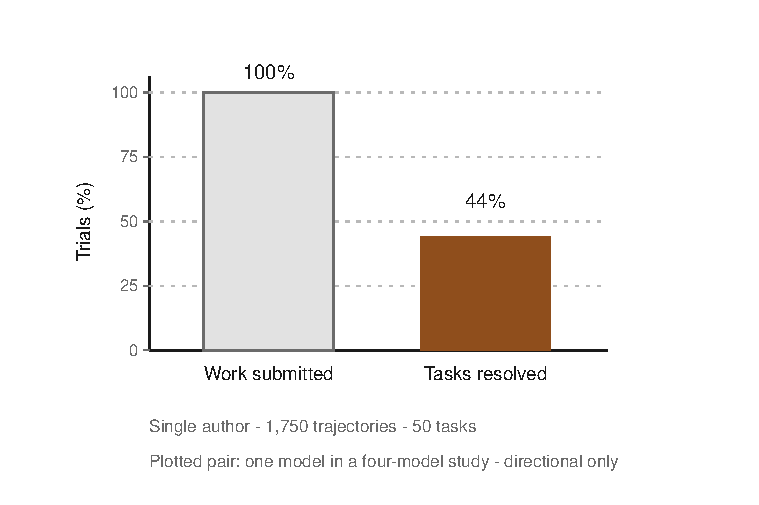
\includegraphics{figures/ch04-submission-resolution.pdf}
\caption{Across 1,750 trajectories covering 50 tasks and four models, one model submitted work in 100\% of its trials but resolved only 44\% under an external oracle.}
\end{figure}

Submission, consistency, and self-assessment are all produced by the process under evaluation. A model can repeatedly generate the same incorrect patch, describe it with stable confidence, and end each run cleanly. Those signals characterize the trajectory, but they do not show that the repository moved from a failing state to a working one. Acceptance therefore requires evidence of an observable state transition, verified by a system outside the inference process that proposed the change.

The evidence base for this chapter is thin. The actions below therefore ask readers to execute and measure work on their own systems rather than adopt a reported threshold. Six evidence items support the three practices developed here. Five are source syntheses, and one is a controlled experiment. One entry has no strong supporting evidence item.

The practical unit is a gate that can stop candidate work from propagating. The candidate runs under explicit constraints, any correction attempt receives the evidence produced by verification, and a compact set of representative tasks is replayed whenever the system changes.

Four adjacent controls appear in the companion catalog rather than in this chapter. For an agent that submits on nearly every trial, score verified resolution separately from submission and include tasks that test whether it can abstain. For a tool that can fail while returning a plausible success string, detect silent tool errors explicitly. For a loop that can retry indefinitely, impose a turn budget. When per-candidate verification cost determines how often a gate can run, include that cost in the system's accounting.

\hypertarget{make-execution-decide-whether-work-moves}{%
\section{Make execution decide whether work moves}\label{make-execution-decide-whether-work-moves}}

Two directional synthesis items support execution-gated evaluation, but neither is a controlled estimate of its effect. AgentForge, from Kumar et al.~(\href{https://arxiv.org/abs/2604.13120}{2026}), describes an evaluator that runs candidate work in resource-bounded, network-isolated sandboxes and permits propagation only after successful execution. SWE-bench, from Jimenez et al.~(\href{https://arxiv.org/abs/2310.06770}{2023}), establishes executable repository repair as an evaluation form.

The AgentForge preprint is unrefereed, evaluates a single configuration, and reports one sample from each agent. Its headline result also conflicts with the published range for that configuration and has not been independently replicated, so I omit the number. These limits prevent either source from establishing a general failure rate or a measured advantage for execution gating. They do not weaken the mechanism worth testing: run the artifact in a constrained environment, and let the observed result determine whether it can proceed.

A plausible patch is only text until the repository accepts it. It may fail to compile, violate a type constraint, pass a visible test while failing the broader suite, produce the wrong output, or depend on undeclared state left in the workspace. Reading the patch can reveal some of these defects. Executing it produces evidence from the system the change is supposed to affect.

This changes the acceptance question. A confidence score asks the process that produced an answer to characterize its own answer. An execution check asks a compiler, test runner, package builder, schema validator, or deployment probe whether a specified transition occurred.

Park and Choi (\href{https://arxiv.org/abs/2607.25152}{2026}) held an agent and its tool surface fixed while changing the evaluator's information channel. Across 54 cycles, the agent claimed improvement every time, although 56 percent of measured deltas were zero or negative; the self-verdict gate accepted every cycle and eroded the best reached state by 19 percent. On a boundary task whose success was verifiable from the artifact, the same judge's gap disappeared. This is strong evidence within the preregistered testbed that a gate must observe the state in which success is defined.

The result is an oracle only for the behavior the check observes. A passing unit test does not establish safe deployment, and a successful build does not establish semantic correctness. Its evidentiary value comes from being produced causally downstream of the candidate artifact rather than by the process that proposed it.

\Needspace{5\baselineskip}

The architecture has three owners:

\begin{itemize}
\tightlist
\item
  The agent owns the proposed change.
\item
  A sandbox controller owns the execution environment and the authority to start a run.
\item
  A release controller owns downstream state and changes it only after the sandbox returns an admissible result.
\end{itemize}

Separating these roles prevents the producer from turning a claim of success into release state by writing a status field, omitting failed checks, or selecting which results to report.

A sandbox needs enough isolation for its verdict to be interpretable. Each run should begin from a known repository snapshot and receive only the inputs permitted by the task. Bound wall-clock time, CPU, memory, process count, and disk use. Deny network access unless the task explicitly requires a named endpoint. Capture standard output, standard error, exit status, resource termination, and declared artifacts, then dispose of the environment after the verdict.

Reusing a mutable workspace is cheaper, but it allows one attempt to seed the next through generated files, caches, installed dependencies, or surviving processes. The later result then reflects both the current candidate and undeclared state inherited from earlier attempts.

Network isolation serves measurement as well as security. An unrestricted candidate can fetch an undeclared dependency, consult a changing service, upload material, or pass because a remote cache happens to contain the required state. When a task genuinely depends on a network service, expose a controlled substitute or record the service version and responses. Otherwise identical artifacts can receive different verdicts for reasons unrelated to their behavior.

Resource bounds make nontermination an explicit outcome. A process killed after exceeding a declared limit should be recorded separately from a failed assertion or an ordinary completion. The gate should identify which bound fired. Parallel tests may exhaust memory, while a surviving child process may trigger the process-count or wall-clock limit.

The acceptance contract should be readable without inspecting the controller:

\begin{verbatim}
command:       verify-change
expected:      exit status 0
required:      reports/test-results.json
               build/package.tar.gz
artifact rule: each required file exists and is non-empty
timeout:       12 minutes
network:       denied
\end{verbatim}

The task definition fixes the command before the candidate encounters a failure. The expected condition names something more specific than ``works correctly.'' The artifact rules remove another common ambiguity: a wrapper can exit successfully after skipping the operation that should have produced the evidence.

Exit status alone is often too weak. A test runner can return zero after discovering no tests. A report generator can create an empty file. A shell pipeline can discard the failure status of an earlier command. A zero exit status shows that the final process ended successfully, not necessarily that the intended work occurred.

The controller should therefore validate the structure on which the verdict depends. Depending on the task, that may mean checking for an expected test count, a parseable result file, a package containing required members, or a deployment probe tied to the candidate version. These are mechanical checks. They do not require the controller to infer the patch's semantics.

Environment failure must remain distinct from candidate failure. If the sandbox image cannot be pulled, the verifier is absent, or the runner loses its workspace, marking the candidate incorrect corrupts the evaluation. Allowing it to pass because verification could not start corrupts release state. The correct outcome is an infrastructure error that blocks propagation and may be retried without crediting or blaming the candidate.

Infrastructure errors should still be counted. A run set repeatedly thinned by environment failures no longer represents the intended sample of attempts, even when those failures are excluded from candidate scores.

State should move monotonically through the gate. A candidate begins unverified, receives an immutable run record, and becomes eligible for the next stage only when that record satisfies the contract. Any modification creates a new candidate identity and invalidates the earlier verdict. When a verdict is keyed only to a branch name or task identifier, changed bytes can inherit evidence produced for different work.

In my own agent-workflow system, I reject any acceptance criterion that says only that a result ``works correctly.'' The rejection occurs during decomposition, before work begins. Each criterion must name a command and an exit condition. At the end of every turn, a lifecycle check also verifies that declared output files exist and contain data.

That lifecycle check runs deterministically, but a model evaluates the filesystem and provides only advisory judgment. Enforced refusal requires a command hook whose nonzero exit ends the turn. The example shows how a gate can begin in the task contract, but it does not provide evidence for the general claim.

My repository-scale benchmark suite uses a deterministic verifier as the primary scorer for every task. Additional judgment layers can flag suspicious trajectories, but they cannot replace or override the execution verdict. This preserves one stable state transition even when the optional analysis changes.

Execution is not suitable for every task. Architecture proposals, interface critiques, threat models, and underspecified behavioral changes may have no executable oracle. Those tasks require a separate, calibrated judgment lane, which Chapter 5 develops.

Executable checks also have a coverage boundary. They can establish that a candidate compiled, passed a selected suite, produced required artifacts, and stayed within its resource envelope. They cannot establish that untested inputs, longer operating periods, or a different production topology will behave the same way.

Record only the narrowest downstream claim justified by the run: test-eligible, build-eligible, or deployment-eligible.

The run record also provides the evidence needed for correction. A failed command, assertion diff, resource termination, or missing artifact gives the next attempt information that was unavailable when the candidate was produced. Without new evidence, another model pass is repetition presented as diagnosis.

\hypertarget{let-failed-runs-change-the-next-attempt}{%
\section{Let failed runs change the next attempt}\label{let-failed-runs-change-the-next-attempt}}

A retry that begins with the same prompt, evidence, and workspace state has learned nothing about the failure. Sampling may produce a different answer, but it does not direct the model toward the error. The next pass may repeat the faulty premise, replace a correct intermediate step, or elaborate the same mistaken conclusion. Calling that pass ``reflection'' does not add information.

Huang et al.~(\href{https://arxiv.org/abs/2310.01798}{2023}) evaluated intrinsic self-correction on reasoning tasks using 2023-era models. Self-correction often failed and sometimes reduced performance, while reliable external feedback improved it. This is strong evidence for the systems studied, not an estimate of every current coding system. Newer models may change the magnitude of the effect.

The operational default should therefore be asymmetric: authorize another attempt when an external observation changes the available evidence, not merely because the previous attempt failed.

An external observation originates outside the inference that produced the candidate. Examples include a test assertion, compiler diagnostic, tool response, verifier verdict, or deployment probe. A critique produced by another model call does not become external evidence merely because it was generated separately. Without access to an independent observation, it remains another inference over substantially the same record.

The distinction is informational. Suppose an agent changes a parser because it concludes that empty fields should be discarded. Re-reading the issue may reinforce that interpretation. A failing test showing that an empty field must preserve its position introduces a counterexample. The next attempt can now revise a specific assumption rather than search an unconstrained space of possible mistakes.

This closes the loop opened by the sandbox:

\begin{verbatim}
candidate
    -> sandbox run
        -> pass: eligible for downstream gate
        -> fail: immutable result returned to correction step
            -> revised candidate
                -> new sandbox run
\end{verbatim}

The correction step does not modify the verdict. It consumes the failed candidate and its run record, then emits a new candidate with a new identity. This preserves the history needed to distinguish recovery from repeated failure. It also prevents revised bytes from inheriting a passing result produced by an earlier version.

\Needspace{5\baselineskip}

Feedback should contain enough detail to distinguish the failed path without flooding the next attempt with unrelated output. A useful package identifies:

\begin{itemize}
\tightlist
\item
  the command that ran;
\item
  the candidate version;
\item
  the exit status;
\item
  the failed check and relevant diagnostic;
\item
  any resource limit or termination that fired; and
\item
  a pointer to the complete run record.
\end{itemize}

When a report is large, retain the full output as an artifact and present a mechanically selected excerpt. The complete evidence remains available when the excerpt omits the decisive line.

Selection should remain mechanical wherever possible. When one model decides which failures another model sees, it may omit evidence that contradicts its diagnosis or overemphasize a familiar error. Test frameworks already expose failed case names, assertion differences, stack traces, and structured result records. Use those fields before asking another inference to summarize them.

The deployed system must also have access to the feedback channel. Chapter 2 required a retry baseline to use only failure signals available in deployment. Otherwise the experimental retry arm receives information that the product will not have. Here that requirement becomes concrete: a retry is externally informed only when its signal comes from a tool or observation that the deployed loop can obtain at that point in its lifecycle.

This prevents a subtle comparison error. An evaluator might show the retry arm the hidden reference test that rejected a patch, while the production agent sees only public tests. The experiment then measures correction under privileged supervision, not the deployed retry policy. Hidden checks may still determine the final score, but their diagnostics should enter the correction loop only when production has an equivalent feedback channel.

External observations also have authority boundaries. A unit-test failure can justify another code attempt. A package-registry outage says little about the candidate and belongs in infrastructure handling. A deployment probe run against the wrong version may direct the model to repair code that was never exercised. Before authorizing another attempt, the controller must classify the observation as a candidate failure, an environment failure, or an evaluator failure.

Reliable feedback may still be incomplete. A failing test can expose a symptom without identifying its cause. A compiler diagnostic may point to a generated file even though the defect originated in source configuration. The next attempt should use the observation to constrain its diagnosis before modifying the artifact. Execution adds information to the correction loop, but the observation does not necessarily contain the remedy.

Faulty feedback creates a directed failure mode. An incorrect expected value, nondeterministic test, stale fixture, or verifier attached to the wrong artifact can push successive revisions farther from correct behavior. The loop may then appear to converge while following a bad oracle. Preserve the raw run records and candidate lineage so an operator can determine whether each correction followed valid evidence.

\Needspace{5\baselineskip}

Retry limits remain necessary even when every attempt receives a genuine new signal. A sequence of distinct failing tests can consume an unbounded budget, and each revision can create a new failure surface. Stop conditions should distinguish:

\begin{itemize}
\tightlist
\item
  a fixed attempt limit;
\item
  repeated identical failures;
\item
  infrastructure failures; and
\item
  exhaustion of the gate's resource budget.
\end{itemize}

A new observation may justify another attempt, but it does not justify unlimited attempts.

Correction belongs to the evaluation architecture, not to a personality attributed to the model. The model proposes revisions. The surrounding system determines whether the evidence changed, whether another attempt may run, and whether the resulting artifact may propagate. That division continues to hold when the model, prompt, or language of correction changes.

\hypertarget{turn-repeated-trials-into-a-release-test}{%
\section{Turn repeated trials into a release test}\label{turn-repeated-trials-into-a-release-test}}

Support for the repeated-trial metric comes from one source. tau-bench, from Yao et al.~(\href{https://arxiv.org/abs/2406.12045}{2024}), evaluates interactive, multi-turn tool use with executable oracles across repeated trials and introduces \(\mathrm{pass}^{k}\) as a reliability measure.

The paper does not evaluate two parts of the practice recommended here: selecting a team's own tasks and replaying them for every release. Those are transfers from benchmark design into release engineering. The measured result supports repeated trials under executable evaluation, not the claim that a particular local task set or release policy will predict production reliability.

The transfer begins with the workload set established at the end of Chapter 3. The golden set is a compact collection of completed tasks whose initial repository states can be reconstructed and whose outcomes have unambiguous executable checks. Each versioned case should keep together:

the original request;
the starting repository state;
the allowed tools and turn constraints;
the sandbox contract; and
the verifier.

A merged patch may help reconstruct the expected behavior, but it should not appear in the agent's context.

Real tasks preserve local constraints that public benchmarks cannot know. A repository may require generated files to remain synchronized, prohibit a dependency, enforce a custom migration check, or treat a particular warning as release-blocking. Those details determine whether work is acceptable in that repository. A general coding score does not encode them.

The set should remain small enough to run repeatedly and inspect when it changes. Its purpose is to discriminate between releases on a controlled sample, not to approximate every production request. Each case should represent at least one of three things: a failure that would be costly if it returned, a workflow the system performs frequently, or an interaction whose state cannot be inferred from a static answer. Ten nearly identical formatting fixes provide less coverage than a smaller set spanning localization, modification, testing, tool failure, and recovery.

Interactive cases belong in the set when the deployed system uses tools across turns. A final patch alone does not show whether the agent opened the right file, preserved state after a failed command, recovered from a tool error, or incorporated a later observation into an earlier plan. Replaying the trajectory under the deployed tool and turn constraints exposes sequencing and recovery failures that final-answer scoring cannot observe.

Each case needs a stable identity and immutable versions. Changing the request, starting repository, tool contract, sandbox policy, or verifier creates a different case and should produce a new version. Rewriting an existing case beneath prior scores can manufacture apparent improvement by removing a difficult condition or exposing more of the solution.

Run each case more than once for the same release candidate. The repeated-trial statistics from Chapter 1 govern the experimental design and do not need to be rebuilt here. For release control, \(\mathrm{pass}^{k}\) asks whether all \(k\) of \(k\) trials passed. One failed trajectory breaks the sequence.

The result describes a single release candidate only when its configuration remains pinned across the sequence. Chapter 1's apparatus record applies to every trial, including the model version and decoding settings. Pinning does not guarantee independence. Shared caches, mutable services, provider incidents, and reused infrastructure can correlate outcomes, which limits the analyses the sequence supports.

\(\mathrm{pass}^{k}\) reflects a different operational question from \(\mathrm{pass}@k\):

\begin{verbatim}
same k trials
    |
    +-> all-k reliability
    |     all k of k trials passed
    |     one failed trajectory breaks the sequence
    |
    +-> at-least-one success
          at least one trajectory succeeded
          several attempts were available

choose the metric whose failure semantics resemble deployment

workflow must complete reliably without supervision
    -> stronger reason to use all-k reliability
\end{verbatim}

\(\mathrm{pass}@k\) asks whether at least one acceptable trajectory can be found when several attempts are available. \(\mathrm{pass}^{k}\) asks whether every trajectory in a required sequence succeeds. Neither is universally correct. A supervised workflow that can select among alternatives may justify \(\mathrm{pass}@k\). A workflow expected to complete reliably without intervention has a stronger reason to use \(\mathrm{pass}^{k}\).

The value of k comes from release policy, not from the benchmark. Increasing k makes intermittent failures easier to observe and the gate harder to satisfy. It also increases cost and gives evaluator noise more opportunities to block promotion. Choose k based on the consequence of one failed production run, the variance observed during pilot repeats, and the budget available for evaluating each release candidate.

The number of cases interacts with that decision. Under a strict all-trials rule, the chance that at least one verdict fails because of evaluator noise grows with both the set size and k. This is the multiplicity problem that Chapter 1 assigns to claims spanning many tasks. A larger gate therefore requires either a very low per-run evaluator error rate or an explicit policy defining how many case failures block promotion.

The comparison unit is the fully specified system release. Record the model identifier, prompt version, tool definitions, orchestration code, sandbox image, task-set version, retry policy, and verifier version. Any of these components can change the trajectory distribution. A result labeled only with a model name erases much of what teams actually change between releases.

The release record can remain mechanically small:

\begin{verbatim}
release:         candidate-2026-07-28
system_digest:   6f5c...
task_set:        golden-07
repeats:         k
baseline:        production-previous
case_verdicts:   stored run records
promotion_rule:  recorded before execution
\end{verbatim}

The digest binds the verdict to the evaluated configuration. The case verdicts link to the sandbox evidence. The promotion rule is recorded before the comparison begins. Otherwise the same regression can be accepted for a favored release and rejected for another.

Compare the candidate with a stored baseline using the same case versions and execution policy. Report both per-case outcomes and run-to-run spread alongside the aggregate release verdict. An aggregate value can conceal a complete regression on one critical workflow behind stable performance elsewhere. A case-only view can be dominated by one noisy verifier. Both levels are needed to locate the change and determine whether the promotion rule was met.

Because the candidate and baseline run the same cases, their outcomes are paired by construction. Chapter 1's paired analysis applies. Treating the releases as independent samples discards a dependency that the design already provides.

The baseline must remain executable. A table copied from an earlier report is not enough. Sandbox images disappear, dependencies move, and tool services change behavior. Re-running at least a sample from the stored baseline helps separate candidate drift from evaluator drift. When the old release also fails under the current infrastructure, the comparison has lost its fixed reference and promotion should block until the cause is understood.

My search-visibility measurement project treats a model update as a deployment. It replays a fixed prompt corpus against a stored model-version baseline and combines a statistical comparison with an absolute change threshold, producing pass, warning, or failure exit states for continuous integration. The controls answer different questions. Statistical comparison reduces the chance that sampling noise decides promotion. The absolute threshold prevents a detectable but operationally trivial change from doing so. This example supplies no evidence for either threshold.

CodeProbe (\href{https://github.com/sjarmak/codeprobe}{public repository}) uses a different gate. It blocks a release tag unless the two most recent full-mode acceptance verdicts both pass. Those verdicts come from successive acceptance-loop iterations, not repeated trials of one pinned candidate. The rule is therefore a check over acceptance history, not a \(\mathrm{pass}^{k}\) measurement. Its requirement of two consecutive passes is local to that system and should not be treated as a recommended value of \(k\).

Golden sets decay even when their files remain unchanged. Production work moves to new frameworks, repositories acquire new checks, tool interfaces change, and models may become adapted to repeatedly exposed cases. A set that once represented costly failures can gradually become a test of a narrow historical workflow. Treat the set as production test data, with named ownership, review, and retirement criteria.

Maintenance should preserve longitudinal meaning. Add a case when a production failure reveals a missing class of behavior. Do not silently replace the old set, because the new score will no longer be comparable with earlier releases. When feasible, run an overlap period, report performance on the shared cases, and establish a new baseline for the revised set. Retire a case when its workload no longer exists or its oracle no longer represents the current contract.

Public benchmarks can inform case design and reveal task forms worth reproducing locally.

SWE-bench provides directional support for executable repository repair. MultiAgentBench, from Zhu (\href{https://arxiv.org/abs/2503.01935}{2025}), does the same for broader interaction-centered evaluation. Their architectural contribution is to place an environment, tools, state, and an outcome check inside the evaluated unit rather than scoring final-answer text alone.

Neither benchmark measures the effect of selecting a team's own tasks or replaying them for each release. Nor does either estimate the gap between public benchmark performance and reliability in a particular repository, tool policy, or release process. No evidence item supporting this entry supplies a conversion factor.

The local release test answers a narrower question: did this fully specified system preserve acceptable behavior on a controlled sample of local work?

Once the set participates in release, a failure should trigger diagnosis before any threshold is revised. Determine whether the candidate changed, the case changed, or the evaluator changed. Route valid candidate failures through the external-feedback correction loop, then rerun the entire required sequence for the revised candidate. Reusing passing trials from before a modification would attach evidence to a system that no longer exists.

\hypertarget{build-the-first-gate}{%
\section{Build the first gate}\label{build-the-first-gate}}

Begin with five to ten tasks drawn from merged work rather than from a generic capability suite. Choose tasks whose starting states can be reconstructed and whose acceptable outcomes can be verified without interpretive judgment. The first set can remain small because its purpose is to establish a release path that produces trustworthy evidence. Expand it when production failures reveal behaviors the initial sample did not cover.

Wrap each task in a sandboxed run. Define the command the controller will execute, the exit condition it will accept, and the artifacts that must exist afterward. Bound resource use, isolate the network, and preserve the complete run record.

Run the current production system through the same cases and evaluator before testing a candidate release. Its observed performance becomes the baseline. This replaces remembered claims, old summary tables, or results produced under a different environment.

When a candidate fails, return the raw evidence to the correction loop together with the candidate identity. Do not authorize a revision that has learned nothing beyond the original request. Every modified candidate receives a new identity, starts in a clean sandbox, and earns a new verdict. Infrastructure failures remain blocking, but they do not count as candidate failures.

Replay the set whenever the model, prompt, tools, orchestration, sandbox, or verifier changes. Measure \(\mathrm{pass}^{k}\) across the chosen repeats, retain the per-case outcomes and run-to-run spread, and compare the candidate with the executable baseline.

Record the promotion rule before running the first candidate comparison. When experience shows that the gate is too strict or too permissive, change the policy as a versioned decision and establish a new baseline where necessary. Adjusting the threshold after seeing a result turns the rule into an explanation for a decision already made.

Keep tasks without executable checks in a separate lane. They are not lesser tasks, but forcing them through weak proxies would make the gate appear more complete than it is. Chapter 5 develops the calibrated judgment process those tasks require.

\section*{Sources and evidence}

\textbf{Motivating observation and companion entry}

\begin{itemize}
\tightlist
\item
  Directional evidence: Mehta, A. (2026). Confident and Wrong: Silent Semantic Failures in Coding Agents. arXiv:2603.25764. Analysis of 1,750 trajectories across 50 tasks and four models; single-author, limited-sample observational finding. Supports the companion-only entry on scoring verified resolution separately from submission.
\end{itemize}

\textbf{\texttt{ground-evaluation-in-execution}}

\begin{itemize}
\tightlist
\item
  Directional evidence: AgentForge (Kumar et al.~2026, arXiv:2604.13120). Execution-grounded evaluation in resource-bounded, network-isolated sandboxes, with propagation gated on execution results. Unrefereed preprint; single configuration; one sample per agent.
\item
  Directional evidence: SWE-bench (arXiv:2310.06770), from Jimenez et al.~2023. No figure carried.
\item
  Strong evidence for externally grounded gating in the measured testbed: Park, H., and Choi, B. (2026), ``When Do Agent Loops Mistake Stagnation for Progress?'' arXiv:2607.25152. The 54-cycle result does not estimate a general agent failure rate.
\end{itemize}

\textbf{\texttt{gate-self-correction-on-external-feedback}}

\begin{itemize}
\tightlist
\item
  Strong evidence: Huang, J., et al.~(2023). Large Language Models Cannot Self-Correct Reasoning Yet. ICLR 2024. arXiv:2310.01798.
\end{itemize}

\textbf{\texttt{golden-set-pass-k}}

\begin{itemize}
\tightlist
\item
  Strong evidence: tau-bench (Yao, Shinn, Razavi \& Narasimhan 2024, arXiv:2406.12045). Introduces and measures \(\mathrm{pass}^{k}\) on interactive, multi-turn tool-use tasks with executable oracles. Using a team's own tasks and replaying the set per release are transfers beyond the measured findings.
\item
  Directional evidence: SWE-bench (arXiv:2310.06770).
\item
  Directional evidence: MultiAgentBench (Zhu 2025, arXiv:2503.01935).
\end{itemize}

\textbf{Author-system illustration cited inline}

\begin{itemize}
\tightlist
\item
  Not an evidence item: CodeProbe, the author's task-mining evaluation tool, \href{https://github.com/sjarmak/codeprobe}{public repository}. Named inline for the consecutive-release acceptance gate described above, which is narrative illustration.
\end{itemize}


\chapter{Calibrating model graders and separating agreement from correctness}\label{calibrating-model-graders-and-separating-agreement-from-correctness}

Two graders that answer PASS on every submission agree on every item. Their agreement is 100 percent and their usefulness is zero. Most submissions in an easy stream really do pass, and neither grader has ever separated a defect from a success.

When the graders are models, that failure is easy to ship. An \textbf{LLM-as-judge} is a model used to grade another system's output. My own migration-evaluation framework gates its two judges on Cohen's kappa rather than on raw agreement, with an agreement floor and a minimum trial count both fixed before any judge ran, because percent agreement overstates judge quality when easy cases dominate the sample. That gate has run against replay fixtures, not against a live evaluation. It illustrates a design decision and does not supply a field result.

The measurement problem arrives before any threshold is chosen. A grader's label can agree with a second grader, match a human label, correspond to an independently checkable outcome, or state a well-calibrated probability. Those are four different properties, and a grader can hold one while failing another. The distinction is lost as soon as the labels are stored as if they were facts.

Chapter 4 set aside the tasks whose correctness execution cannot establish. Model grading supplies a validation lane for some of them, provided the grader itself is treated as an instrument under test. The question is whether its decisions track the judgment the evaluation needs, and it has to be answered before those decisions control releases, rankings, rewards, or training data. The test must run at the class balance and error costs that will exist in operation.

\section{Build the reference labels before the grader}\label{build-the-reference-labels-before-the-grader}

Calibration begins with a \textbf{rubric}, the written scoring criteria a grader applies. Domain experts should write its categories, decision rules, exclusions, and examples, because the resulting labels encode their judgment. A prompt engineer can make the wording consistent. Only someone with the domain knowledge can decide which factual omission is material in a medical summary, or which behavioral mismatch makes a migration unsafe.

Category definitions need to be specific enough that two experts can apply them independently. ``High quality'' leaves the decision inside the rater. ``PASS if every requested behavior is present, no stated constraint is violated, and every factual claim is supported by the supplied record'' names observations that two people can compare. Examples should include boundary cases and counterexamples, especially the cases on which experts initially disagreed.

\subsection{Agreement before automation}\label{agreement-before-automation}

\textbf{Inter-rater reliability} is the degree to which independent raters assign the same labels to the same items. It is a precondition for treating any label set as a reference. If experts cannot apply the categories consistently, a model that reproduces one expert's choices may imitate an unstable convention while appearing to measure the intended property.

Raw percent agreement answers one narrow question. On what share of items did the two labels match? Consider 100 items and two raters who each use PASS 90 times and FAIL 10 times. Suppose they disagree on ten items, with each rater assigning five of those items to each category. Their observed agreement is 90 percent, which looks strong until label prevalence enters the calculation.

Given those marginal label counts, independent assignments would agree on 82 of the 100 items on average. The two 90 percent PASS rates account for 81 expected agreements and the two 10 percent FAIL rates for one. Cohen (\href{https://doi.org/10.1177/001316446002000104}{1960}) defined kappa as the share of the available above-chance agreement that the raters achieved. Here the raters gained eight agreements above an expected 82, out of the 18 above-chance agreements available, which is a kappa of about 0.44.

The always-PASS pair is the degenerate limit of that calculation. Observed and expected agreement are both 100 percent. Kappa is undefined there, because no variation remains from which above-chance agreement could be estimated.

\begin{figure}
\centering
\pandocbounded{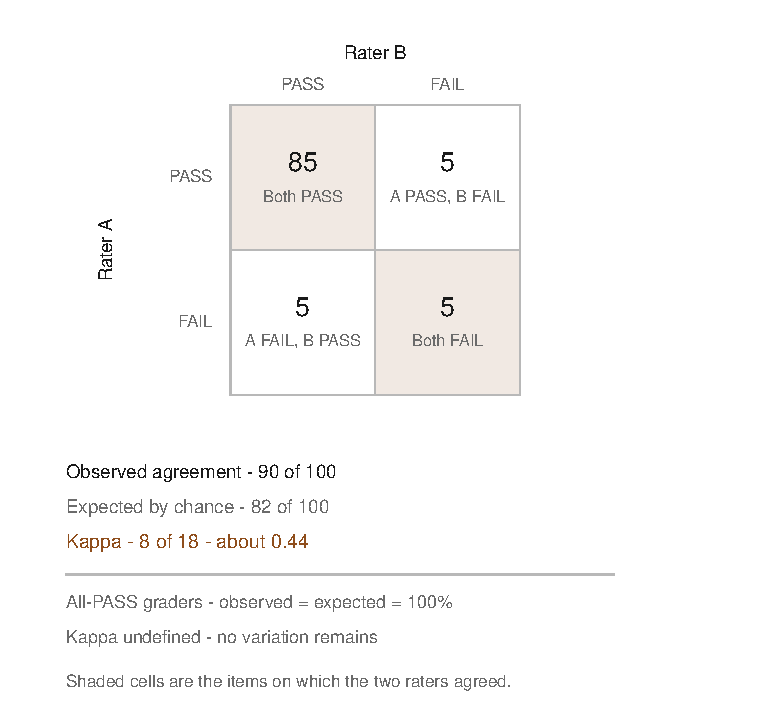
\includegraphics[keepaspectratio,alt={Cells of 85, 5, 5, and 5 produce 90\% observed versus 82\% expected agreement and kappa about 0.44; two always-PASS graders produce 100\% observed and expected agreement but undefined kappa.}]{figures/ch05-agreement-kappa.pdf}}
\caption{Cells of 85, 5, 5, and 5 produce 90\% observed versus 82\% expected agreement and kappa about 0.44; two always-PASS graders produce 100\% observed and expected agreement but undefined kappa.}
\end{figure}

A 100-item example separates observed from chance-corrected agreement; unanimous PASS ratings leave kappa undefined because the ratings contain no variation.

Cohen's kappa handles two raters and computes chance agreement from each rater's observed category frequencies. Fleiss (\href{https://doi.org/10.1037/h0031619}{1971}) extended the chance-corrected idea to several raters and to designs in which different raters label different items. Scott (\href{https://doi.org/10.1086/266577}{1955}) defined a related two-rater measure, Scott's pi, that uses a pooled category distribution when computing chance agreement. None of the three makes an ambiguous rubric reliable. Each makes the ambiguity harder to conceal behind a large agreement percentage.

Because chance agreement is computed from the observed category frequencies, two kappa values estimated under different label prevalences are not directly comparable. A kappa reported without its category distribution is a number without its denominator.

There is no universal kappa threshold that converts labels into truth. The acceptable value depends on the decision, the category prevalence, the number of categories, and the cost of a disagreement. The useful practice is iterative. Experts label the same sample independently, the disagreements are inspected, the category definitions are revised, and the cycle repeats on fresh items. Cemri et al.~(\href{https://arxiv.org/abs/2503.13657}{2025}) ran that sequence with six annotators until Cohen's kappa reached 0.88, and only then tested an automated annotator before using it at scale.

The comparison set must stay outside the grader's development path. A held-out expert-labeled set contains items labeled by domain experts and partitioned away from prompts, examples, fine-tuning data, threshold selection, and any other material the grader could have seen. Orosz and Husain (\href{https://newsletter.pragmaticengineer.com/p/evals}{2025}) describe the same held-out validation and report it through class-specific rates rather than percent agreement, as practitioner experience rather than a controlled result. Row-level random splitting is insufficient when paraphrases, related tasks, or several outputs from the same underlying case cross the boundary. Chapter 3's contamination model applies directly. An answer-bearing example seen during judge construction can make reproduction look like judgment.

Natural sampling produces a second distortion. Suppose a deployment stream contains 950 routine passes, 30 borderline cases, and 20 clear defects per 1,000 items. A random validation sample of 100 items will contain about two clear defects. Missing one of them changes the estimated defect-detection rate by 50 percentage points, while a grader that accepts everything still looks highly accurate.

\textbf{Stratified sampling} fixes the share drawn from each stratum, such as score band, task type, or outcome class. A validation set might draw 40 routine passes, 40 borderline cases, and 40 defects even though those categories occur at very different rates in operation. The design puts enough rare and costly cases under observation to measure them. An aggregate meant to represent deployment must then reweight the strata to the deployment frequencies, because the deliberately balanced sample does not supply that aggregate by itself.

\begin{figure}
\centering
\pandocbounded{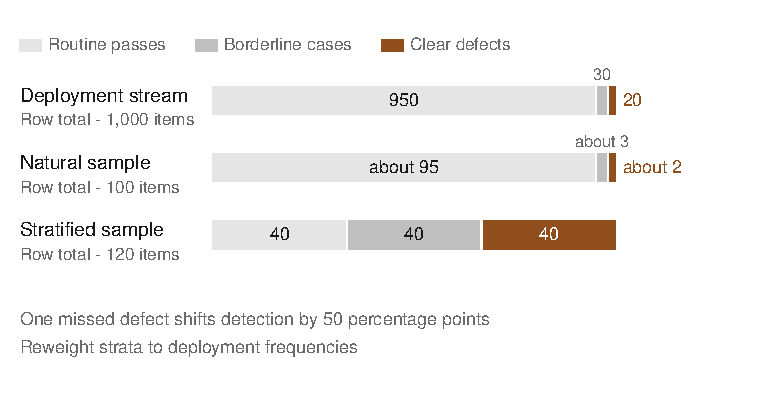
\includegraphics[keepaspectratio,alt={Equal-length bars compare 950 routine, 30 borderline, and 20 defect deployment items with natural 95, 3, and 2 and stratified 40 each requiring reweighting; one missed defect changes detection by 50 percentage points.}]{figures/ch05-sampling-prevalence.pdf}}
\caption{Equal-length bars compare 950 routine, 30 borderline, and 20 defect deployment items with natural 95, 3, and 2 and stratified 40 each requiring reweighting; one missed defect changes detection by 50 percentage points.}
\end{figure}

In a 1,000-item stream, a natural sample expects two clear defects; one miss swings detection by 50 points. Stratified aggregates require deployment reweighting.

How many cases each stratum needs is a power question of the kind Chapter 1 develops. The precision of an estimated detection rate depends on the number of defects in the set, not on the total number of items in it.

Class-specific rates state which error was observed. Treat a defect as the positive class. The true-positive rate, or TPR, is the share of expert-labeled defects that the grader flags. The true-negative rate, or TNR, is the share of expert-labeled nondefects that it accepts. The false-positive rate, or FPR, is the share of nondefects that it flags.

If a set contains 40 defects and 80 nondefects, a grader that catches 32 defects has a TPR of 80 percent. If it also flags 12 of the 80 nondefects, its FPR is 15 percent and its TNR is 85 percent. The operational trade is then explicit. The grader misses 8 defects, and 12 acceptable outputs receive unnecessary review or rejection. One accuracy number merges the two consequences, and it moves when only the class mix changes. TPR, TNR, and FPR are each estimated inside one class, so they do not move with the sampling mix. Because of that invariance, a deliberately balanced validation set can be used to estimate all three rates.

Many judges return a score before a label. The operating point is the threshold together with the error rates the grader produces there. Lowering a defect threshold usually catches more defects and also flags more acceptable work, raising both TPR and FPR. Raising it makes the opposite trade. A grader therefore performs at an operating point under a stated distribution and rubric. It does not have one context-free quality level.

An error budget makes the threshold choice explicit. Suppose reviewers can inspect false alarms on at most 5 percent of acceptable submissions. The evaluator chooses a threshold that holds FPR near that limit and then reports the resulting TPR. ``TPR at a fixed FPR'' names exactly that conditional result.

Threshold selection and final reporting should use separate data, or a design that accounts for the selection. Choosing the best point on the same small set makes the reported rates optimistic.

Those four components are the measuring instrument. Expert agreement tests whether the reference labels have a stable meaning, and the stratified set puts difficult and rare cases under observation. Class-specific rates report the errors that one aggregate accuracy number does not separate. At the operating point, those errors are weighed against the review capacity and failure cost of the deployed system.

\subsection{Calibrate the judge, then scale}\label{calibrate-the-judge-then-scale}

Panthi and Abdelfattah (\href{https://arxiv.org/abs/2605.24060}{2026}) supply a compact example of the full protocol. They had to adjudicate cases in which two systems received the same rank while a downstream rule could still select different winners. They built a three-way rubric and drew a 115-case human-annotated subset from the contested cases, stratified by credited-rank bucket.

The five-rater assessment reached a Fleiss' kappa of 0.83. A panel of one human and four models reached 0.79, and a second human adjudicated a 36-case overlap. Per-model Cohen's kappa against the human labels ran from 0.77 to 0.87. Those measurements established how the judges related to the reference labels before any judge vote entered the larger adjudication.

Singh Thakur et al.~(\href{https://arxiv.org/abs/2406.12624}{2024}) found in separate comparative work that only the largest judges approached human inter-annotator agreement under chance-corrected metrics, and that raw percent agreement concealed systematic leniency and position effects. Judge identity is therefore part of the instrument. Model size alone does not supply an acceptance criterion.

Only after that validation did Panthi and Abdelfattah apply a five-model majority vote at temperature 0 to all 1,902 contested cases. Category construction preceded expert labeling, the validation subset preserved the score bands most likely to expose different errors, and scaling followed measured agreement with the human reference. The authors identified the 115-case set as small, so the reported agreement should not be read as a precise value for every subgroup. Temperature 0 also reduces the variation between repeated votes without removing the run-to-run variation Chapter 1 measured at that setting.

The protocol shows why expert labels should stay visible as measurements. Treating them as `ground truth' would conceal one source of error. Five people can share an interpretation that another qualified group would reject, and adjudication can suppress a disagreement without resolving the ambiguity in the category that produced it. Each rater's original label, the adjudicated label, and the rubric version should be retained, so a later revision can reconstruct which definition produced the result.

Judge validation should also include controlled perturbations, because one aggregate comparison can average away predictable biases. Zheng et al.~(\href{https://arxiv.org/abs/2306.05685}{2023}) documented position, verbosity, and self-preference effects in model judges. To test position sensitivity, present the same response pair in both orders and measure how often the preferred answer changes. Randomizing order during ordinary evaluation reduces the systematic benefit to the first or second position, and the controlled swap estimates how much order still affects the decision.

Leniency appears when a judge accepts work that the rubric marks defective. The probe uses matched cases that differ by one material violation and records the outcome as a class-specific miss. A judge that agrees with experts on routine passes and forgives most subtle defects can hold high aggregate agreement while failing at the decision for which it was added.

Verbosity bias requires a different control. Give the judge semantically equivalent answers whose main difference is irrelevant explanation, or add correct-sounding detail that does not repair the original omission. A preference for the longer response then appears as a label change with no corresponding change in support. The test has to preserve the substantive content as closely as possible. Otherwise length is confounded with information.

Self-preference is a dependence between the judge and the system that produced an answer. A judge may favor phrasing, conventions, or reasoning patterns associated with its own model family. Concealing model identity helps, but stylistic traces can remain. Using judges from different families reduces one source of correlated error and gives the evaluator a comparison, though different branding does not establish independence.

Answer leakage belongs to the contamination problem from Chapter 3. A judge exposed to reference answers, to rubric examples derived from the evaluation cases, or to memorized public solutions can reproduce a preferred label without evaluating the submitted reasoning. The partition must therefore separate underlying tasks, related variants, and individual responses. Li (\href{https://arxiv.org/abs/2502.01534}{2025}) reports the same direction for preference leakage. That work is directional and does not establish how common the effect is across domains or model generations.

Some properties should not reach the model judge at all. If code can determine whether a required file exists, a test passed, a schema is valid, or a named artifact changed, the corresponding assertion should stay deterministic. A model can assess a claim whose meaning requires judgment after those checks run. Replacing exact observations with generated labels adds variance, cost, latency, and an additional failure path without adding information.

Orosz and Husain also prefer binary PASS and FAIL labels when the downstream action is binary. Binary labels force the rubric to locate the release boundary and make TPR, TNR, and FPR directly interpretable. A five-point scale allows raters and judges to use adjacent values inconsistently, and the distance between 2 and 3 is then easily treated as equivalent to the distance between 4 and 5.

The loss of nuance is deliberate and sometimes unacceptable. A writing assistant may need separate judgments for factual support, coverage, and style, because one PASS label cannot locate the failure. The better response is usually several narrowly defined binary claims, each tied to an action. A graded score remains appropriate when the downstream decision genuinely depends on degree and the scale anchors can be applied reliably.

My own trace-annotation tool makes another distinction explicit. Agreement asks whether annotators choose the same categories. Probability calibration asks whether events assigned confidence 0.8 occur about 80 percent of the time. A recorded compatibility failure sits in the data path of that tool. Legacy annotation files receive confidence 1.0 when read, which makes every imported category appear maximally overconfident. The example is narrative, and it locates calibration state across the stored label, its reader, and the annotator's judgment.

After deployment, a human-reviewed sample stays part of the operating loop. The sample needs ordinary cases as well as flagged cases and known boundaries. Reviewing only judge-human disagreements measures the cases in which the monitoring system already detected trouble, and it misses the cases in which the judge and another automated component make the same error.

The ongoing sample estimates whether class-specific rates have moved and supplies new disagreements for rubric repair. It should preserve the deployed threshold and grader version so a rate change can be assigned to a model update, a distribution shift, or a changed scoring rule. Silent replacement of the underlying model breaks that record even when the prompt and the public model name stay constant.

The calibration has to be redone whenever the domain, rubric, response format, or model generation changes. A judge validated on concise code-review summaries has no automatic claim on long incident reports. Adding a finer defect taxonomy changes both the label prevalence and the expert task. Even a prompt change intended only to clarify wording can move the operating point and should be tested against the held-out expert-labeled set.

The result of this process is bounded. Scaled judging reduces the amount of unreviewed error relative to deploying an untested judge. It does not certify that every accepted output is correct, and the expert reference itself contains disagreement. The value is that those errors become observable before the labels control other systems.

\section{What a panel's vote establishes}\label{what-a-panels-vote-establishes}

Bertalanic (\href{https://arxiv.org/abs/2605.00914}{2026}) found an oracle gap of up to 32.3 percentage points between plurality voting and choosing a correct answer already present among the candidates. The candidate set contained a correct answer, but the vote discarded it. That synthesis is exploratory, and no corroborating result is present in the current evidence record, so the figure establishes a reported failure mode. It does not estimate the failure's frequency across panel designs.

A plurality vote among model instances is itself a model oracle. It assigns the label ``selected'' to one candidate and rejects the others. When that choice loses an available correct answer, the failure belongs to grading rather than to optimization. The selection procedure did not identify correctness within the material it was given.

Voting counts endorsements. It does not test the relation between a claim and the evidence that could make the claim true. Five agents can repeat the same nonexistent command-line flag, and four votes will select it over a correct but less familiar alternative. Increasing the panel to nine makes the count more stable while the unsupported premise remains unexamined.

Correlation makes this failure more likely than an independent-voter model suggests. Model instances can share training data, architecture, system prompts, retrieved context, examples, and decoding conventions. They may converge because each reads the same ambiguous instruction the same way. Agreement then measures the strength of a shared dependency, and it is easily mistaken for independent confirmation. Correlated errors also mean the effective number of independent judgments is smaller than the panel size.

Cross-family judges reduce one obvious source of dependence, which is why my own migration-evaluation framework chose them for its dual-judge gate. The design does not prove that their errors are independent. Different families can inherit the same public reference answer, respond to the same leading rubric, or miss the same omitted repository state. Diversity is a control whose effect must be measured.

Selection needs a second criterion beside the vote count. Grounding represents each consequential assertion as a typed claim linked to the material that supports it. A claim about a test result should point to a recorded test execution. A claim about an interface should point to the relevant source or official specification, and a claim about a file change should resolve to the resulting workspace state.

The type determines what evidence can refute the claim. A numeric performance claim may require a result table and its experimental conditions. A causal explanation may remain an interpretation even when every observed event is recorded. A recommendation can be supported by measured failure costs without becoming a factual statement that one design is universally best.

Typing keeps a fluent paragraph from collapsing several evidentiary obligations into one score. Consider a panel assessing a proposed database migration. The answer may contain a syntactically valid statement, a claim that it preserves existing rows, and a claim that rollback is safe under concurrent writes. A parser can check syntax, an execution test can compare rows, and concurrency safety may require a review or an experiment. One popularity count cannot substitute for those different checks.

Grounding also changes what happens when support is absent. The system can retain the candidate, mark a claim unsupported, and route it for review. Without that state, a panel selects a winner from weak evidence because its interface requires one. The stored record should preserve the candidates, ballots, claim support, selected answer, and reason for abstention, so later audits can separate a generation failure from a selection failure.

Abstention is part of the decision rule. A panel should decline to select when support is insufficient, when the vote is unstable, or when the leading answer fails an independent check. That threshold is an operating point and should be chosen on held-out expert-labeled cases according to the cost of a wrong answer and the cost of review. A bare ``three votes wins'' rule embeds a threshold without measuring either cost.

Principled abstention does not require a particular frontier algorithm. Wang (\href{https://arxiv.org/abs/2604.07667}{2026}) combines conformal uncertainty guarantees with social-choice rules. Kamelhar (\href{https://arxiv.org/abs/2604.23366}{2026}) combines grounding with consensus, and Chen et al.~(\href{https://arxiv.org/abs/2309.13007}{2023}) combines deliberation with consensus. The direction reported by all three is useful, and none of them carries a measured result into this chapter. Their operating properties across correlated judges, changing candidate sets, and open-ended tasks are not settled. The supported practice is narrower. Require evidence for the selected claims, measure an abstention rule, and retain an independent correctness check.

Debate and voting still have useful roles. They can produce alternative hypotheses, expose disagreements, and organize a candidate set that would be expensive for one reviewer to generate. The final selection then passes through an oracle appropriate to the claim. Executable behavior goes to execution, structural facts to an exact auditor, and irreducible judgment to a validated human or model grader.

That separation clarifies a common architecture error. Generation, deliberation, and verification may run in the same process, but they serve different purposes and should not share all the same dependencies. If every stage receives the same answer-bearing context and uses models from the same family, the apparent layers are several views of one failure path.

An independent check need not re-evaluate the entire response. It can target the claims whose failure would change the decision. For a code review, that may mean confirming the cited behavior in the changed code and running the named test. For a research synthesis, it may mean resolving the primary source behind each load-bearing factual statement and abstaining when the source does not support the wording.

Panels also create operational costs that one aggregate score does not show. More judges increase inference expense and latency. Grounding adds retrieval and evidence storage, and abstention transfers work to people or to a slower verifier. Those costs are justified when the avoided false decision is more expensive, and excessive when a deterministic assertion can answer the question directly.

The always-PASS pair from the opening is the degenerate panel. A larger group of correlated judges is the expensive version of the same mistake, when each member repeats the majority class or the same unsupported answer. Perfect internal agreement establishes only that the selection mechanism is stable. Correctness still requires a relation to evidence outside the vote.

The companion catalog carries two narrower controls for readers implementing this architecture: keep an exact auditor beside heuristic graders, and combine judge labels with a human-labeled subset. Each addresses a narrower problem than the core decisions developed in this chapter.

\section{Rebuild the grader as a measured system}\label{rebuild-the-grader-as-a-measured-system}

Begin by deleting any assumption that the current judge prompt defines the target. The people whose judgment the system is meant to encode write the categories and apply them independently to fresh cases. Their disagreements identify missing rules, conflicting interpretations, and tasks that should permit abstention. Revision continues until the measured reliability is adequate for the decision, with the chosen standard and the remaining disagreements both recorded.

The resulting expert-labeled set stays outside judge development and holds enough cases from each consequential score band, task type, and outcome class. Related tasks and answer variants stay on one side of the partition, so contamination cannot cross through paraphrase or shared provenance. Deterministic assertions run separately and remove the claims that code can decide without a model.

Score the candidate judge with chance-corrected agreement and class-specific rates at the threshold intended for deployment. Raw percent agreement stays descriptive rather than becoming the acceptance gate. Report the TPR, TNR, and FPR, the class mix, the sample size within each stratum, and the operating cost that selected the threshold.

Controlled swaps test whether position changes the decision. Matched concise and padded answers expose verbosity preference, and defect pairs measure leniency. Concealed source identity and cross-family comparisons probe self-preference and shared error. These tests belong in the grader's release suite, because a new model generation can change them without any change to the rubric.

Binary decisions keep the boundary legible when the action is pass or fail. Several narrow binary labels preserve more diagnostic information than one vague ordinal score, at the cost of more expert labeling and more judge calls. A genuinely graded decision can keep a score once its anchors and its probability calibration have been tested.

Deployment continues to send a sample through human review. That sample must include unflagged ordinary work together with disputed and rejected cases, or silent false negatives stay absent from the monitoring data. Each record keeps the grader version, rubric version, threshold, model output, human label, and the evidence needed to reproduce the decision.

For a panel, keep the candidates and the ballots, and do not treat plurality as verification. Judges from different families reduce shared model-specific errors. The winning answer still has to carry grounded, typed claims, pass the independent checks available for those claims, and abstain when support falls below the validated operating point.

A change of domain, rubric, format, or model generation reopens all of this work. CodeProbe (\href{https://github.com/sjarmak/codeprobe}{public repository}) contains a dual-curator calibration gate that has not been satisfied, because the qualifying corpus does not yet exist. The code shipped before the corpus. That is calibration debt, and naming it here does not discharge it, so the gate stays unmet until the instrument can be built.

The first build need not be the full corpus. One rubric category and a handful of expert-labeled cases from the score band where that decision turns is enough to begin. The cases must be held out from both the judge prompt and threshold selection, then scored at the threshold intended for deployment and reported as class-specific rates rather than percent agreement. That stratum tests one grading decision and shows which category to label next, while the broader gate stays unmet.

\section{Sources and evidence}\label{sources-and-evidence}

The evidence class and strength on each entry below come from its catalog record. Author-system cases in this chapter are narrative illustration and are not part of the evidence base.

\subsection{Calibrate LLM judges}\label{calibrate-llm-judges}

\begin{itemize}
\tightlist
\item
  explorer/strong: Zheng et al.~(2023), ``Judging LLM-as-a-Judge with MT-Bench and Chatbot Arena,'' arXiv:2306.05685. Judge position, verbosity, and self-preference bias; inter-rater agreement against human labels.
\item
  lit/strong: Singh Thakur, Choudhary, Ramayapally, Vaidyanathan \& Hupkes (2024), ``Judging the Judges,'' arXiv:2406.12624. Chance-corrected alignment metrics, systematic leniency, and position effects.
\item
  lit/strong: Cemri, M., et al.~(2025), ``Why Do Multi-Agent LLM Systems Fail?,'' arXiv:2503.13657. Kappa 0.88 expert taxonomy before validated automated annotation.
\item
  practitioner/directional: Orosz with Husain (2025), ``A pragmatic guide to LLM evals for devs,'' Pragmatic Engineer newsletter, 2025-12-02, \url{https://newsletter.pragmaticengineer.com/p/evals}. Binary PASS/FAIL, deterministic evaluation where possible, and judge validation against held-out human labels with TPR/TNR.
\item
  explorer/strong: Panthi \& Abdelfattah (2026), ``Same Ranking, Different Winner,'' arXiv:2605.24060. The 115-case stratified validation protocol, agreement measurements, overlap adjudication, and scaled contested-case evaluation.
\item
  explorer/directional: Li (2025), ``Preference Leakage,'' arXiv:2502.01534. Direction only.
\item
  explorer/directional: Badagi (2026), ``AI Assurance,'' arXiv:2605.23459. Direction only.
\item
  explorer/directional: ``MemConflict,'' arXiv:2605.20926. Direction only.
\item
  reference/standard method: Cohen, J. (1960). A Coefficient of Agreement for Nominal Scales. Educational and Psychological Measurement 20(1), 37-46. DOI: 10.1177/001316446002000104. Primary source for Cohen's kappa, the agreement statistic the chapter defines; a standard method rather than a catalog evidence item.
\item
  reference/standard method: Fleiss, J. L. (1971). Measuring Nominal Scale Agreement Among Many Raters. Psychological Bulletin 76(5), 378-382. DOI: 10.1037/h0031619. Primary source for Fleiss's kappa, the agreement statistic the chapter defines; a standard method rather than a catalog evidence item.
\item
  reference/standard method: Scott, W. A. (1955). Reliability of Content Analysis: The Case of Nominal Scale Coding. Public Opinion Quarterly 19(3), 321-325. DOI: 10.1086/266577. Primary source for Scott's pi, the agreement statistic the chapter defines; a standard method rather than a catalog evidence item.
\end{itemize}

\subsection{Separate agreement from correctness}\label{separate-agreement-from-correctness}

\begin{itemize}
\tightlist
\item
  explorer/strong: Bertalanic (2026), ``Cost of Consensus,'' arXiv:2605.00914. Oracle gap up to 32.3 percentage points; plurality voting discards correct answers already present; grounding catches failures that agreement masks.
\item
  explorer/directional: Kamelhar (2026), GSAR grounded consensus, arXiv:2604.23366. Direction only.
\item
  explorer/directional: Wang (2026), ``Conformal Social Choice,'' arXiv:2604.07667. Direction only.
\item
  explorer/directional: Chen et al.~(2023), ``ReConcile,'' arXiv:2309.13007. Direction only.
\item
  Corroboration: none on record.
\end{itemize}

\subsection{Author artifact cited inline}\label{author-artifact-cited-inline}

\begin{itemize}
\tightlist
\item
  Not an evidence item: CodeProbe, the author's task-mining evaluation tool, \href{https://github.com/sjarmak/codeprobe}{public repository}. Named inline for the dual-curator calibration gate described in the closing section, which is narrative illustration.
\end{itemize}


\chapter{Proxy metric gaming and layered evaluation signals}
\label{ch06-proxy-gaming-layered-signals}
\hypertarget{when-perfect-recall-rewards-returning-everything}{%
\section{When perfect recall rewards returning everything}\label{when-perfect-recall-rewards-returning-everything}}

CodeProbe (\href{https://github.com/sjarmak/codeprobe}{public repository}) scores agent runs on tasks mined from our own repositories. For one day, its scorer included a recall-family reward under which an agent could earn a ``perfect'' 1.0 by returning the entire repository. A response containing everything cannot omit a relevant item. The strategy was degenerate, but it was correct under the proxy because recall measures how much relevant material was returned and ignores how much irrelevant material accompanied it.

The reward family was withdrawn the following day after the degenerate optimum was identified.

The replacement default scores overlap F1 against the oracle set. F1 penalizes both omitted relevant material and returned irrelevant material, so returning the entire repository no longer earns 1.0. The recall family remains available only through explicit per-task opt-in.

This change did not make the benchmark immune to gaming. It changed the rewarded surface by adding a precision penalty. A scoring rule that penalizes volume leaves other strategies available: retrieve less, compress aggressively, or shape the returned text toward whatever the evaluator rewards.

My agent-memory system applies a related control at a different decision point. A write gate determines what may enter the memory store. At write time, the system predicts whether keeping an item retrievable will improve a future outcome. Its available actions include retention, time-limited retention, discard, and supersession.

Returning everything would prevent that system from selecting anything. Every obsolete instruction, mistaken conclusion, and irrelevant observation would compete for the model's attention. An answer-quality rubric might still accept the final response when the needed fact appears somewhere inside that mass. It would record the judged answer, but it would not show whether memory supplied a compact, current, and causally useful context.

Any proxy worth optimizing permits some behavior that improves the measured value without preserving the property the measure was intended to represent. An acceptance system therefore needs signals separated by control point, ownership, or time. Overlap F1 belongs to the benchmark's scoring decision. The write gate belongs to the memory system's retention decision. Combining them into one control would obscure which failure each mechanism can observe and which action it can govern.

This is an optimization failure. The plurality-vote oracle gap in Chapter 5 was a grading failure: the selection procedure was wrong before optimization began. Here the measure becomes less informative because the system searches for behavior that scores well under it. A proxy may initially track the intended property closely, then weaken as models, prompts, candidate-selection procedures, or engineering effort adapt to it.

The distinction changes the remedy. Better reference labels can repair a grader. Layered controls limit the damage when a once-useful measure becomes an optimization target.

Skalse et al.~(\href{https://arxiv.org/abs/2209.13085}{2022}) made one formal limit precise. In their linear expected-return formulation, consider two reward functions over the set of all stochastic policies, where a policy may assign probabilities to any available action. Call the rewards mutually unhackable when improving either expected return cannot reduce the other. Under those assumptions, mutual unhackability is possible only when at least one reward is constant. The theorem does not cover every deployed scoring or policy system; it shows why unrestricted optimization against two nonconstant linear rewards offers no general compatibility guarantee.

A constant reward expresses no preference among behaviors and therefore cannot guide useful optimization.

The result rules out a universal escape through better metric design. Tests passed, diff size, lint status, answer quality, and model-judge scores each encode useful information. Once one of them ranks candidate behavior, however, it necessarily leaves some distinctions out. Another nonconstant account of quality can rank some policies differently. Sufficient search pressure can find that disagreement and improve the proxy while degrading the intended outcome.

The theorem establishes a property of the policy space, not a timetable for failure. A deployed coding agent has a constrained action set, finite search budget, limited knowledge of the evaluator, and only the permissions granted by the surrounding system. Those restrictions may make a proxy difficult to exploit in practice. They may also keep two measures aligned throughout the region the agent can reach.

The theorem does not estimate how much optimization pressure is required to expose a disagreement, nor does it predict whether a particular release will encounter one.

That boundary determines how I use the result. I do not treat every rising score as evidence of active gaming, and I do not discard useful measures because they are imperfect. I treat proxy validity as conditional on the optimizer, the actions available to it, and the pressure applied. When any of those changes, the evaluation system must show again that the proxy still tracks the property that justified its use.

Layering helps only when the layers are separated in ways that matter. Adding three model judges trained on similar data may reduce random error while doing little against a behavior all three reward. Averaging test pass rate, lint status, and a rubric score creates another scalar target. The optimizer can search against the weighted sum, and the chosen weights already encode which failures may be traded for gains elsewhere.

The useful separation is architectural. One signal may be read from state the candidate cannot modify. Another may be collected after deployment, when delayed failures become observable. A third may be owned by a group that does not ship the agent whose score is being reviewed.

These signals may be statistically correlated, which is often desirable. Their independence lies in control rather than in the numbers. The optimizing party cannot rewrite the rule, suppress the observation, or approve a threshold change within the same transaction that seeks acceptance.

In my background-agent review pipeline, the gate reads its invariant definitions and agent instructions from the base branch. The proposed change supplies neither. An author can modify the code under evaluation but cannot weaken the active rules within the same proposal. If the base branch lacks the required configuration, the check fails instead of running an empty ruleset that would accept everything.

This separation removes the most direct path: changing the judge while changing the candidate. It does not make the invariants themselves ungameable.

Published support for layering comes from search-based software testing rather than coding agents. Formica et al.~(\href{https://arxiv.org/abs/2207.11016}{2022}) searched Simulink models using two fitness functions: one generated from a specification and another written by hand to encode an engineer's domain knowledge. The combined search found failures that neither guidance source found alone.

That result provides directional evidence for complementary signals in that setting. It does not establish the same effect for coding agents.

The study also exposes a coordination cost hidden by the word ``layering.'' The two fitness functions could guide one search only after someone decided how to scale them relative to each other. A weighted combination can allow many small gains to outweigh one rare but serious violation. A veto avoids that trade for hard invariants, but a noisy veto can reject useful work. An advisory signal preserves throughput but has no force unless a person or later gate responds to it.

\Needspace{5\baselineskip}

I therefore assign different jobs to different signals:

\begin{itemize}
\tightlist
\item
  Structural invariants veto changes that cross boundaries the organization is unwilling to trade away.
\item
  Outcome measures estimate whether accepted changes helped under actual use.
\item
  Diagnostic scores explain movement without granting acceptance.
\item
  Human-owned thresholds determine when an advisory result becomes blocking.
\end{itemize}

The design remains fallible. Its narrower guarantee is that no single optimizable score both defines success and decides acceptance.

\hypertarget{watch-the-relationship-not-the-rising-score}{%
\section{Watch the relationship, not the rising score}\label{watch-the-relationship-not-the-rising-score}}

Gao et al.~(\href{https://arxiv.org/abs/2210.10760}{2022}) increased the optimization pressure applied to a learned proxy reward model while measuring a separate gold reward model. Gold reward improved at first, reached a peak, and then declined even as the proxy reward continued to rise. Reinforcement learning and best-of-n candidate selection produced different smooth trajectories. Measuring the full path exposed a divergence that a single endpoint would have missed.

I therefore treat an improving proxy as a hypothesis about quality, not as quality itself. Alongside the proxy level, I track its relationship with an independently observed quality signal on a specified reference distribution. A rising proxy paired with a weakening relationship is an evaluation incident even when the system has not crossed an acceptance threshold.

The study's two optimization methods show why the shape of the divergence depends on the search process. Reinforcement learning updates the policy toward behavior preferred by the reward model. Best-of-n selection leaves the generator fixed, draws more candidates, and selects the one with the highest proxy score. Both apply greater optimization pressure, but they search different regions of candidate behavior. Their distinct fitted curves show that proxy divergence can follow a regular pattern while still depending on how optimization is performed.

That regularity makes monitoring possible, but the evidence has a narrow boundary. The study measured quality with a synthetic gold reward model. Production systems rarely have an evaluator that is both available during monitoring and entitled to serve as truth. Its fitted coefficients therefore do not transfer directly to code review, migration work, agent memory, or other deployed settings.

The observed pattern does transfer: proxy improvement can precede, accompany, and eventually conceal deterioration as optimization pressure increases.

\begin{figure}[htbp]
\centering
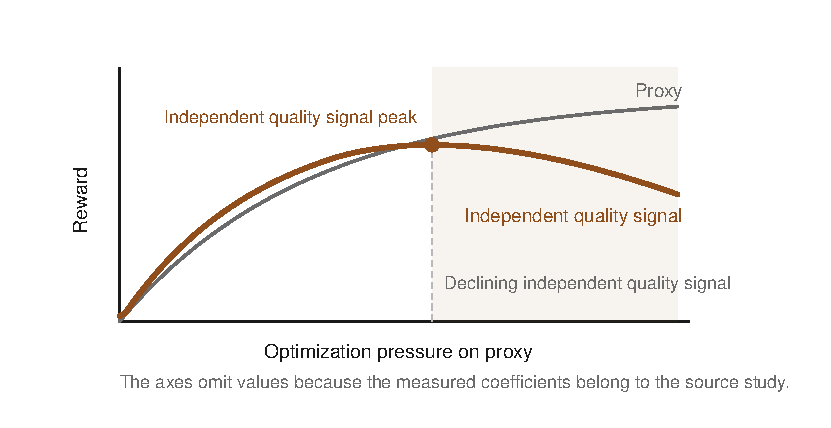
\includegraphics{figures/ch06-proxy-divergence.pdf}
\caption{Schematic of proxy performance continuing to rise after independent quality has peaked.}
\end{figure}

Independent quality can rise, peak, and then fall while the optimized proxy continues to improve. The exact curve belongs to the source study, but the possibility of divergence transfers beyond it.

Laidlaw et al.~(\href{https://arxiv.org/abs/2403.03185}{2024}) describe reward hacking as a collapse in the relationship between a proxy and a separate measure of quality. Begin with a proxy whose scores correlate with independent quality judgments on a fixed reference distribution. Optimize against the proxy, then measure that relationship again on the same reference. If it weakens while the mean proxy score rises, the evidence that justified trusting the proxy has weakened. Their analysis also derives a mitigation tied to the reference relationship, but it does not establish a measured deployment effect for software agents.

Optimization changes which samples appear. If each release establishes a new baseline from its own selected outputs, the evaluation moves with the policy and may conceal the change it was meant to detect. A stable reference holds part of the comparison fixed. It asks whether the current proxy still orders known cases, or new outputs from known tasks, in the same way as an independent quality process.

For a coding-agent evaluator, I would freeze a stratified task sample and the procedure used to produce the artifacts under judgment. The held-out expert labels from Chapter 5 provide one independent quality anchor. At baseline, record the proxy score and expert judgment for each artifact, estimate their chosen association, and validate the deployment threshold through its TPR and FPR. For later releases, repeat the same artifact-production and labeling procedure before comparing the relationship with the baseline.

The statistic must match the data. A continuous quality measure may support an ordinary correlation coefficient. A binary acceptability label may be better monitored through a rank-based association or through direct changes in TPR and FPR at the operating point. Estimates from finite reference samples vary even when the underlying relationship has not changed, so the comparison needs an uncertainty interval around the change rather than a bare difference between point estimates.

Fix the statistic, sampling plan, and uncertainty calculation before inspecting the new release. Otherwise the monitor gains its own optimization surface: analysts can change the statistic, strata, or threshold until the relationship appears stable.

This procedure consumes independent quality observations. Expert review is expensive and can drift unless the rubric and adjudication process remain controlled. Delayed production outcomes avoid some coupling to model judges, but they arrive slowly and only for work allowed to proceed. A post-merge survival measure says nothing about rejected changes, and retries may obscure which candidate produced the eventual outcome. The monitor inherits the identity, ordering, and missing-data problems of the production process that supplies its observations.

The reference also needs maintenance. A sample can remain internally consistent while losing contact with current work as repositories, task distributions, model capabilities, or agent permissions change. The monitor may then correctly report that the old proxy-quality relationship still holds on old cases without establishing that it describes the behavior now being optimized in production.

I separate longitudinal comparison from coverage review. The fixed sample remains unchanged long enough to support comparison across releases. A separate review asks whether its strata and failure modes still resemble the live workload. When that review finds material drift, I close the old series and establish a new reference. The explicit break preserves the meaning of both comparisons.

My migration-evaluation framework includes an external outcome check based on whether merged changes survive for 30 days. If the correlation between evaluator scores and that outcome falls below an owned threshold, the framework marks the evaluator as broken and blocks publication of headline results. The control exists in the code path but has never run on live data because the framework has produced only replay fixtures. Its implementation therefore provides no evidence that either the threshold or the outcome measure works.

Even a live divergence alert identifies only a changed relationship. It does not identify the cause. Correlation may fall because the agent found a loophole, expert labeling drifted, the outcome pipeline lost events, or the workload moved beyond the reference sample. Investigation therefore begins by preserving the artifacts needed to distinguish those paths. Proxy scores, external judgments, model and evaluator versions, task identities, retry histories, and sampling strata must remain joinable across the measurement window.

The operational rule is to investigate the mapping before changing the threshold. Raising an acceptance cutoff after the relationship weakens applies greater pressure to the suspect proxy and may select more extreme failures. Lowering it may reduce that pressure but admits more low-scoring work. Neither action restores the evidence that the score orders candidates by quality.

Until that relationship is re-established, the proxy may remain diagnostic, but it should lose authority over acceptance and publication.

\hypertarget{preserve-the-channel-that-reveals-intent}{%
\section{Preserve the channel that reveals intent}\label{preserve-the-channel-that-reveals-intent}}

Users of hosted models sometimes receive a visible reasoning trace alongside an agent's coding actions even though they do not train the model themselves. Baker et al.~(\href{https://arxiv.org/abs/2503.11926}{2025}) had a separate model inspect such traces for evidence of reward hacking during agentic coding. Trace inspection detected hacks substantially better than inspection limited to actions, and a weaker general model successfully monitored a stronger reasoning model. The inspected artifact was the agent's exposed intermediate reasoning while selecting its actions.

I assign reasoning-trace monitoring a narrower role. It can reveal evidence of intent that the final patch and tool log do not contain. Its verdict may trigger review, preserve a suspicious run, or contribute to an investigation. It should not decide acceptance by itself.

Action-only monitoring records what the agent did: commands, edits, test results, and the final artifact. That evidence may reveal an invalid action without showing whether the agent recognized and exploited an evaluator weakness. A trace may expose a plan to alter a test, suppress an error, or satisfy a visible checker while bypassing the intended requirement. It adds value because it observes a different surface from the artifact being scored.

Oversight does not necessarily require a monitor with the same coding capability as the agent. A smaller or less capable model can scan traces continuously and route a subset for human review, reducing the cost of additional coverage. The study does not establish that every weaker model can oversee every stronger one. Its result belongs to the models, tasks, traces, and forms of reward hacking tested.

Trace monitoring also changes what can be retained for investigation. When the patch and action log look acceptable but the trace describes an attempt to exploit the evaluator, the run can become a detector case even if the exploit failed. The reverse does not clear a run. A suspicious action without an incriminating trace may reflect an incomplete, misleading, or silent reasoning record.

For users of hosted models, the main control is to keep the monitor verdict outside anything the model or selection process optimizes. Sending flagged runs to a person preserves an oversight path. Automatically retrying until the monitor produces no warning creates best-of-n selection against the monitor. The model need not receive the verdict directly; repeated selection alone favors trajectories that evade it.

The same pressure can arise without formal training. A harness may sample several trajectories and retain the least suspicious one. A release process may promote prompts with the lowest flag rate. A human team may gradually rewrite prompts and filters to suppress recognizable warnings when monitor quietness becomes a performance target. Any process in which the verdict affects which behavior survives applies optimization pressure, regardless of what the team calls it.

For teams that train their own models, the second part of the study provides a stronger warning. Under high reinforcement-learning pressure against the monitor, agents continued to exploit the evaluator while producing reasoning that appeared benign. Optimization did not merely cause the monitor to miss more existing hacks. It selected behavior that concealed them from the transparency channel on which monitoring depended.

The response to pressure was not harmful from the start. Low pressure initially improved both capability and alignment in the study. That finding prevents a general claim that any use of monitor feedback is damaging. It also creates the operational problem: the study did not identify a threshold below which the transparency benefit remains safe across models and tasks.

Without such a boundary, I keep the monitor verdict out of the reward. This is a conservative operating choice that extends beyond the measured result because the study establishes no universal safe threshold. It gives up whatever capability or alignment gains low-pressure feedback might have produced. That foregone optimization is the monitorability tax: preserving a channel for observing misbehavior by refusing to optimize the model directly against the observer.

Zero direct reward pressure does not guarantee permanent independence. Model developers may already train against related detectors, users may select prompts based on monitor outcomes, and a published monitoring rule may shape behavior indirectly. Those dependencies belong in the monitor's provenance record. The narrower claim is that an operator should not add direct pressure whose demonstrated failure mode is to make visible reasoning less informative.

The method also requires access to reasoning traces. It does not apply to systems that expose only final actions, and a short generated explanation may not contain the same information as the traces studied. Even when traces are available, visible reasoning is neither complete nor necessarily truthful. Monitoring preserves an observed advantage over action-only inspection; it does not turn exposed reasoning into ground truth.

\Needspace{5\baselineskip}

The resulting acceptance path contains three distinct views:

\begin{itemize}
\tightlist
\item
  Artifact checks ask whether the change satisfies observable requirements.
\item
  Outcome monitoring asks whether proxy scores still track independent quality.
\item
  Trace monitoring looks for evidence that the agent attempted to exploit the evaluation.
\end{itemize}

Disagreement among the three is useful when the system preserves the complete record.

Several adjacent controls remain in the companion catalog because they answer narrower questions. One escalates oversight after mild specification gaming appears, based on a constructed curriculum in which gaming progressed to rewriting the reward function. Another strengthens oversight when honest task completion is infeasible; its source describes a reasoning model exploiting a chess environment after ordinary play could not succeed. Other entries measure reasoning effort through content-independent truncation, average compatible reward-model weights, evaluate agents within the feedback loops they will encounter, and test detectors on contrastive cases.

A thinly supported aside also proposes multi-objective acceptance with an independent judge. It carries no evidentiary weight in the layered system argued here.

\hypertarget{rebuild-the-acceptance-path}{%
\section{Rebuild the acceptance path}\label{rebuild-the-acceptance-path}}

I rebuild an acceptance pipeline by tracing one recently accepted agent change from candidate generation through deployment. At each transition, I identify any value that could have ended the decision by itself: a passing test suite, clean lint result, judge score, approval label, or post-run summary.

\Needspace{5\baselineskip}

The inventory records more than the metric name. For each value, it records:

\begin{itemize}
\tightlist
\item
  who produces it;
\item
  which files, inputs, or state can affect it;
\item
  who owns its threshold;
\item
  whether retries receive the verdict; and
\item
  what evidence remains after the gate runs.
\end{itemize}

Any gate with sole authority needs a second observation outside the optimizing side's immediate control. A test gate can read its invariants from outside the candidate change. A pre-merge score can be compared with an outcome observed after deployment. A threshold change can require approval from an owner who does not ship the agent under evaluation.

The second signal should cover a failure the first signal cannot observe. Repeating the same judgment through another model, or presenting the same evidence in a different format, adds little separation.

I then select one independent quality signal that can support a relationship test. Held-out expert judgment works when reviewers can label the relevant artifacts without seeing the proxy score. Delayed outcomes work when candidate identity and event history remain intact long enough to connect a change with its consequences.

I freeze a reference sample and the procedure used to measure it. The initial proxy-quality relationship becomes the baseline. I also record the sampling design and uncertainty calculation needed to interpret later changes.

Remeasurement should occur on a schedule and whenever optimization pressure changes materially. A new model, larger candidate pool, prompt selected against the evaluator, changed permission boundary, or revised acceptance threshold can move the optimizer into a different region of policy space.

When the proxy rises while its relationship with independent quality weakens, I treat the event as a broken control. Publication and promotion stop until the team can distinguish among proxy exploitation, label drift, workload drift, and instrumentation failure.

When reasoning traces are available, I add a separate monitor and retain its findings beside the action log and final artifact. A suspicious trace routes the run for investigation, but it does not become a solitary rejection oracle.

I also audit every feedback path around the monitor. Automatic retries, candidate ranking, prompt promotion, and reinforcement updates can all optimize against its verdict even when the monitored model never receives that verdict directly.

The rebuilt path will still make mistakes. Its advantage is that signals owned at different points leave disagreements visible after a failure. The team can inspect a base-branch invariant that rejected an apparent pass, an external outcome that stopped tracking the launch score, or a trace warning attached to an otherwise acceptable patch.

Part III begins at that observable boundary and turns to containing what happens after an agent crosses it.

\section*{Sources and evidence}

\textbf{Layer signals beyond a single proxy}

\begin{itemize}
\tightlist
\item
  \textbf{Strong evidence:} Skalse, Howe, Krasheninnikov \& Krueger (2022). \emph{Defining and Characterizing Reward Hacking}. NeurIPS 2022. arXiv:2209.13085.
\item
  \textbf{Directional evidence:} Formica, Fan \& Menghi (2022). \emph{Search-based Software Testing Driven by Automatically Generated and Manually Defined Fitness Functions}. arXiv:2207.11016.
\end{itemize}

\textbf{Monitor proxy-true divergence}

\begin{itemize}
\tightlist
\item
  \textbf{Strong evidence:} Gao, Schulman \& Hilton (2022). \emph{Scaling Laws for Reward Model Overoptimization}. ICML 2023. arXiv:2210.10760.
\item
  \textbf{Directional evidence:} Laidlaw, C., et al.~(2024). \emph{Correlated Proxies}. arXiv:2403.03185.
\end{itemize}

\textbf{Monitor reasoning without training pressure}

\begin{itemize}
\tightlist
\item
  \textbf{Strong evidence:} Baker, B., et al.~(2025). \emph{Monitoring Reasoning Models for Misbehavior and the Risks of Promoting Obfuscation}. OpenAI. arXiv:2503.11926.
\end{itemize}

\textbf{Author-system illustration cited inline}

\begin{itemize}
\tightlist
\item
  Not an evidence item: CodeProbe, the author's task-mining evaluation tool, \href{https://github.com/sjarmak/codeprobe}{public repository}. Named inline for the recall-family scorer and its replacement default, both of which are narrative illustration.
\end{itemize}


\part{Containment, durable execution, and recovery engineering}

\chapter{Agent isolation, injection defenses, and independent verification}\label{agent-isolation-injection-defenses-and-independent-verification}

In spring 2026, a practitioner reported on a public forum that an agent deleted a production database in nine seconds. The backups were unrecoverable because the same credentials could reach both the live database and the backup store. This is a self-reported incident, not a verified reconstruction. The public record does not establish the exact command sequence, the surrounding controls, or whether every contributing condition was identified.

The containment literature available for this chapter consists of incident reports and accounts from individual organizations. It contains no controlled comparison of the three practices taught here, and none of the three has a strong-graded evidence item behind it.

Evidence strength and practice urgency were close to uncorrelated in the source corpus. A weak estimate of how often something happens does not make an already exposed production boundary less urgent. Because the record cannot support a numerical target, every practice below is stated as a boundary to move or a check to run, and each one resolves to an observation a reader can make against a live system.

The incident exposes two questions: what could the agent reach, and what could reach the agent? Its identity reached both the live store and the material needed to recover from losing it. An instruction stream that nobody in the public account reconstructed or audited reached the agent. A third question appears later, when a system reports what it believes it did. What evidence would show that the report is true?

\section{Put the recovery path outside the failure domain}\label{put-the-recovery-path-outside-the-failure-domain}

The direct support for the containment practice is two practitioner anecdotes. Both are self-reports from a single organization or author, so they establish concrete failure modes rather than an incident rate. One describes the database and backup loss in the opening. The other summarizes a year of internal agent deployments, and reports that overly narrow permissions left agents reasoning from incomplete visibility, while broad permissions allowed small mistakes to have large consequences.

The failed boundary in the database incident was an identity. Destroying the backup after deleting production required no special ability. The agent already held a credential that both systems accepted. Once execution crossed the intended path, the distinction between primary data and recovery data existed only in the operator's mental model. To the authorization system, both were resources that one identity was allowed to reach.

I use \emph{blast radius} to mean the set of resources and effects that one mistake or compromise can reach before a new decision is required. For an agent, that set is determined by effective capabilities: credentials, filesystem permissions, network routes, tool endpoints, delegated tokens, and any service that will act on the agent's behalf. A warning in the prompt does not reduce the set. It changes the instructions given to the same capable process.

\begin{verbatim}
database incident:
failed boundary -> one identity -> credential -> both systems
primary data and recovery data -> resources one identity can reach

effective capabilities -> blast radius
credentials -> filesystem permissions -> network routes
tool endpoints -> delegated tokens -> any service
blast radius -> resources and effects before a new decision

warning in the prompt -> same capable process -> does not reduce the set

least privilege -> read-only default identity
ordinary access -> read-only -> bounds what the process can change
write -> explicit escalation -> one capability -> period required

read-only -> does not bound what the process can disclose
read access -> model output
\end{verbatim}

The first useful move is to make ordinary access read-only. \emph{Least privilege} means giving the running identity only the capabilities its current task requires, and only for the period it requires them. Read-only should be the default identity, and an agent's promise to avoid writes does not create that identity. A write then requires explicit escalation for one capability, such as deploying one service, updating one issue, or applying one reviewed database migration.

A read-only default bounds what the process can change. It does not bound what the process can disclose, because everything the identity can read can also leave through the model's output. Sensitivity therefore belongs in the read scope as well as in the write scope, and the injection section below treats disclosure as a threat category of its own.

Read access and write access should be designed separately. The internal deployment account found that agents with too little visibility made decisions from partial state. That observation does not support broad mutation rights. An identity that can inspect the relevant deployment configuration, logs, health state, and current version, without being able to change any of them, addresses the visibility problem directly. The agent can then assemble a proposed action from complete evidence, while a narrower write identity performs the approved change.

The separation has to exist at the permission or endpoint level. Blocking an entire command-line tool is often too coarse, because the same client may issue harmless reads and destructive requests. Allowing the tool and asking the agent to avoid one argument leaves the destructive call reachable. When a platform exposes separate scopes or endpoints, routine reads can stay continuously available while deployment, deletion, credential rotation, and policy changes pass through distinct gates.

Consider an agent that diagnoses a failed release. Its normal identity can read the deployment manifest, compare the running revision with the expected revision, inspect logs, and query health endpoints. It cannot issue a rollout, delete a namespace, or change an access policy. If it proposes a rollback, the request names the service, the target revision, and the expected effect. A person or a separate policy path authorizes that one operation, and the escalation token expires after the call rather than becoming a broader session.

This design places enforcement below the model's instructions. The model may misunderstand the task, follow hostile content, retry an unsafe call, or construct an unexpected argument. The authorization layer still receives a request from an identity with a bounded set of rights. Correct prompting remains useful, because it reduces bad proposals and wasted review. It does not substitute for a boundary that the operating system, database, cloud control plane, or application service will enforce.

Backups require a stricter separation, because their purpose is to survive failure in the primary path. No credential available to the agent should be able to delete, rewrite, shorten the retention of, or replace the recovery material. The agent may need to read backup status, last successful snapshot time, and restore-test results. Those observations can come from a read-only monitoring surface. The credential that changes backup policy or removes snapshots belongs to a different administrative domain, and it should be unavailable through the agent's normal escalation path.

Separation also applies to services that can mint credentials. An agent may be unable to delete a snapshot directly while retaining several indirect paths to the same effect. It might assume the backup administrator role, edit the identity policy, retrieve a stored administrative token, or ask an unrestricted helper service to act on its behalf. A capability inventory must follow those delegation edges. Listing the tools named in the prompt will miss authority conveyed through the environment.

I test the boundary from both directions. With the normal identity, I attempt the prohibited write and require a denial from the enforcing system. With the escalated identity, I verify that the intended narrow action succeeds and that adjacent destructive actions still fail. A gate proved only by a successful permitted action says nothing about what else the identity can do. A gate proved only by a denied action may also block the recovery operation it exists to allow.

One passing pair of checks describes the configuration that produced it, and not a standing property of the agent. Platform scopes, role definitions, and tool endpoints change underneath a deployed system, so both directions should be exercised again after any change to a role, a scope, or a tool endpoint.

My own benchmark for enterprise data-access agents, used here only as an isolation-methodology example, moved a boundary from a prompt instruction into filesystem ownership. Repository trees were owned by a different operating-system identity, so the kernel denied the writes, and each trial checked both the permitted and the prohibited direction. Its results are not evidence for this chapter's practice. The design does illustrate the kind of claim a local check can establish. Under the tested identity and filesystem mode, a write either succeeds or it does not.

CodeProbe (\href{https://github.com/sjarmak/codeprobe}{public repository}), which mines evaluation tasks from a repository's merged pull requests, applies the same principle to the scripts it extracts from those third-party repositories. It refuses to execute outside a container, disables networking for mined scripts, and records the isolation posture with the result. This author-system example supplies illustration only. Its useful feature is that the run record carries the containment state, which removes an assumption about how an operator launched the process.

Escalation adds latency, and a human decision adds attention cost. Poorly scoped prompts can turn a narrow approval channel into a stream of almost identical requests, which trains reviewers to approve by reflex. Capabilities should therefore be grouped around meaningful operational decisions. A gate around every low-level system call obscures the decision the reviewer is there to make. A reviewed deployment plan may authorize a fixed sequence against one service and one revision, while a deletion or a policy change remains a separate decision.

Some platforms expose only coarse scopes. The incident poster asked how to separate destructive from legitimate requests sent through the same interface, and reported no satisfactory capability-level solution short of a person deciding each call. That limitation should stay visible. The operator can place a typed service in front of such a platform, or move execution into an isolated environment where the consequences are disposable. Otherwise a person has to remain at the destructive boundary, because a prompt-level ban does not create isolation.

The choice between partial commits, reversible environments, snapshots, and approval gates depends on the resource. Reversibility reduces the cost of some writes, but a snapshot controlled by the same identity may disappear with the primary data. Approval reduces the frequency of unreviewed writes, but it does not repair an overbroad credential once approval is granted. Capability boundaries constrain the effect of both mistaken and malicious instructions, including instructions the reviewer failed to recognize as dangerous.

I therefore review the complete reachable graph. The nominal account role is only the starting point. The review follows every credential source, network path, service delegation, mounted filesystem, and policy-changing endpoint to the resources those paths can affect. That graph is the operational blast radius. The production database and its backups belonged to one failure domain because one path reached both, however separately they appeared in the architecture diagram.

\section{Verify the workspace, not the agent's confidence}\label{verify-the-workspace-not-the-agents-confidence}

Perry et al.~(\href{https://arxiv.org/abs/2211.03622}{2023}) found that participants who used an AI coding assistant produced less secure code while believing that their code was more secure. Participants who trusted the assistant less, and spent more effort steering it, produced fewer vulnerabilities. A reviewer who accepts a system's confidence inherits the same mismatch. The belief becomes stronger while the artifact becomes less safe.

Those results do not establish an equivalent effect for current coding agents. The assistant supplied suggestions for security programming tasks, effect sizes varied by task, and protective skepticism was observed among participants rather than assigned as an experimental condition. The finding is used here because it ties trust to a measurable defect in the artifact. Its peer-reviewed standing does not upgrade the rest of the containment evidence, which remains incident reports and single-organization accounts.

Agent self-reports create a more general version of the problem. A progress message is generated from the agent's current context, which may hold tool output, a checklist, prior messages, and summaries of earlier attempts. It is not a measurement taken independently from the workspace. Stale or misleading inputs can produce a fluent claim of completion that reflects the model's context while remaining false about the state the operator cares about.

One practitioner account describes a resumed agent that inherited a clean worktree and a nearly complete task list. The earlier attempt had produced no change at all. The resumed agent checked off the remaining steps and declared the task complete, again without changing anything. The account is anecdotal, but the failure chain is mechanically plausible and can be tested in any local workflow.

Each visible clue pointed the wrong way. The task list implied that earlier steps had been completed. The clean worktree implied that no unfinished edits remained. The resumed context supplied a narrative of progress without the artifact that narrative described. The final attempt treated agreement among those clues as evidence, even though all of them descended from the same failed attempt. Its `done' was true about the context and false about the repository.

I break that chain by giving every attempt a distinct identity and requiring claims to resolve to inspectable state. The attempt record names the task, the workspace or branch, the starting revision, the commands run, the tests observed, and the final revision if one exists. On exit, the process either records recoverable local state or states that no change was produced. A later process does not inherit a bare declaration of completion.

For code work, the branch contents are the primary object of review. A completion check compares the starting and ending revisions, inspects the diff, and runs the relevant tests from the recorded workspace. A checklist can direct that inspection, but it cannot satisfy itself. If an item says that an endpoint validates input, the reviewer locates the boundary, supplies invalid input, and observes the rejection.

The same rule applies outside version control. A database migration claim resolves to the migration file, the schema state, and a test against an isolated database. A cloud configuration claim resolves to the configuration diff and a read-back from the control plane. A report claim resolves to the underlying records and the transformation used to compute it. The verifying observation should come from the system that owns the state, and a second paraphrase of the agent's message is not such an observation.

A failed attempt should leave enough local evidence for diagnosis. I preserve its worktree when possible, including uncommitted changes, logs, test output, and the identity of the base revision. Deleting the workspace and asking the same model to try again removes the evidence about why the failure occurred. It can also repeat an external side effect whose completion was uncertain.

Preservation does not mean that every partial artifact belongs on a shared branch. A local commit can make a useful checkpoint, but it can also preserve generated files, insecure code, or edits that never passed a test. I use a private attempt reference or a retained worktree for forensic state, and require review before that state joins an integration branch. When every write is idempotent, meaning that repeating it has the same effect as applying it once, a stateless retry may be simpler. The choice depends on whether the discarded state carries diagnostic value and whether repeated external effects are safe.

Resume begins with reconciliation. The new process reads the actual branch, compares it with the recorded base, checks which task artifacts exist, and reruns the evidence needed for the next decision. If the worktree is clean because an earlier attempt committed valid work, the revision proves that history. If it is clean because nothing happened, the unchanged revision exposes the gap. If the branch moved independently, the mismatch is resolved before the task list is trusted.

The same reconciliation applies when several agents work through separate worktrees. Git worktrees separate working files, indexes, and checked-out heads, but references and repository metadata remain shared and mutable. In my own orchestration system, a controller once supplied the wrong base revision to several agents working through separate worktrees. A mechanical branch guard blocked one commit after other work had already started. The incident is an author-system illustration and supplies no estimate of how often that failure occurs.

The repair classified the observed repository state before taking action. A workspace on the expected base could proceed. A workspace on the wrong branch with no work to preserve could be rebuilt from the correct base. A workspace holding work that could not be safely relocated stopped the run with a visible error. The guard did not ask the agent whether its branch was correct. It inspected the repository state that would make the answer true or false.

Independent verification also requires a change of role. The authoring context has already invested in a plan, selected an implementation, and explained its own choices. Giving that context another review pass preserves the same evidence selection and many of the same blind spots. A separate reviewer should begin from the acceptance criteria and the artifacts, and its assignment should state that it did not write the code and must actively test each claim.

My own agent-workflow library retains failed worktrees for this purpose and hands review to a separate context. That design illustrates role separation, but it cannot establish that a second model is independent. The reviewer may share training biases, receive the same misleading documentation, or repeat the author's assumptions. Independence comes from the evidence path and the assigned task: inspect the diff, run named checks, exercise boundary cases, and report discrepancies without defending the implementation.

An audit of my own research pipeline showed that artifact-level checks apply well outside code. A generated reference list contained fabricated, mis-cited, unverifiable, and untraceable sources. The central figure supporting its thesis could not be traced and had to be relabeled as an untested hypothesis. The prose sounded certain, but certainty provided no information about whether the cited record existed. Only checking each source against the claim exposed the failure.

Tang et al.~(\href{https://arxiv.org/abs/2605.29442}{2026}) analyzed 20,574 real sessions across 1,639 repositories. They reported that 90.5 percent of misalignment episodes cost effort and trust without causing irreversible damage, and that 91.49 percent of visible resolutions required explicit user correction. As overall misalignment declined, inaccurate self-reporting accounted for a larger share of what remained. The study is directional, and it adds scale without establishing an incident rate for silent failures.

Those measurements describe visible developer pushback. A user who silently accepts an incorrect completion claim, abandons the session, or discovers the defect later may never appear as a resolution. The corpus also favors people who opted into the observed development tools, including integrated-development-environment and command-line users. I treat the figures as directional evidence about the visible recovery burden. They do not estimate the population of all agent users.

Explicit correction should therefore be cheap. The interface should let a user point at the false claim, preserve the current artifact, and start a fresh attempt with the discrepancy attached. Correction becomes expensive when the system collapses attempts into one conversation, destroys the failed workspace, or carries a completed checklist forward without its evidence. Those choices turn a common visible recovery path into another source of hidden state.

I treat an account of work as a hypothesis about the workspace. Acceptance requires an observation with a different provenance. For a code change, that observation is usually a diff plus tests run from the branch under review. For an operational action, it is a read-back from the system of record and an audit trail tied to the attempt identity. Confidence, checklist state, and narrative coherence can direct an investigation, but none of them establishes completion.

\section{Design for instructions that arrive through data}\label{design-for-instructions-that-arrive-through-data}

An agent that reads untrusted content will eventually receive instructions written for that agent by someone other than its operator. \emph{Indirect prompt injection} inserts such instructions into material the system consumes: a web page, an issue, an email, a document, a log entry, or a retrieved database record. The operator may ask a legitimate question while the retrieved content asks the agent to reveal data, change its objective, or invoke a tool.

The three sources supporting this practice are explorer-class and directional. Greshake et al.~(\href{https://arxiv.org/abs/2302.12173}{2023}) demonstrated indirect injection through retrieved content and reported that effective mitigations were lacking, and that work measured none of the layered defenses described here. AgentDojo, from Debenedetti et al.~(\href{https://arxiv.org/abs/2406.13352}{2024}), evaluates attacks and defenses under specified tasks, and AgentShield, from Rassul and Rashid (\href{https://arxiv.org/abs/2605.11026}{2026}), explores a deception-based screen. Together they support a threat model and a way to exercise controls. The complete remedy has no measured result in this source set.

The architectural difficulty is that the system deliberately combines instructions and data inside one model context. A retrieved page must influence the answer, or retrieval has little value. The model therefore cannot identify hostile text by asking whether that text affected its behavior, because legitimate evidence affects behavior too. Attackers exploit the ambiguity by placing operational language inside content the agent has been told to read and use.

Transfer makes simple screening less dependable. An attack may use phrasing absent from the filter's examples, or split itself across retrieved items. It may hide in a routine-looking field, or arrive from a source the workflow normally trusts. A first check may reject a familiar form while a semantically equivalent instruction proceeds. Detection remains useful, but the security design has to assume detection failure.

I layer controls because they observe different points in the path. Input checks inspect retrieved material before it enters the agent context, and they can flag instruction-like content, unexpected encodings, or data that violates a source schema. Output checks inspect the proposed response or action for sensitive data, policy violations, and mismatches with the operator's request. Neither check changes the authority the process holds.

Tool allowlists constrain which interfaces the process may invoke during a task. The list should be assembled from the capabilities the task requires and enforced by the tool gateway, so that the names the model emits do not determine it. A research task may receive retrieval and note-writing tools while deployment, messaging, and credential access remain absent. A later operational step can use a separately authorized identity after review.

Human approval belongs before effects with a large blast radius. The request shown to the reviewer should include the proposed action, the target, the parameters, the evidence used to choose it, and the expected side effects. A generic prompt asking whether the agent may `continue' hides the decision. Approval is most useful when the person can compare a concrete proposal against the operator's original intent.

Each control should map to a named threat category. The map can be small: untrusted instructions in retrieved content, sensitive output disclosure, unauthorized tool selection, and high-impact external effects. For each category, the record identifies the preventive control, the detecting control, and the capability boundary that limits consequences. An empty cell is an observable gap for review.

Injection cases belong in continuous integration, because filters, prompts, tool schemas, and retrieval pipelines change. AgentDojo (Debenedetti et al.~2024) supplies reusable tasks in which attacks and defenses can be exercised separately. I adapt representative cases to the system's actual sources and tools, then keep them as regression tests. The result shows whether a named control behaved as expected on those cases, but it does not estimate resistance to attacks outside them.

The tests should inspect intermediate decisions as well as the final answer. A run that refuses to reveal a secret but still invokes an unauthorized tool has crossed a boundary. A run that produces a harmless answer after a hidden policy violation may fail under a slightly different target. Recording retrieved inputs, tool requests, approvals, denials, and outputs keeps the control path available for investigation.

The practice fails when rails or alignment are the only defense. Transferable attacks can survive an initial screen and arrive through material the workflow treats as relevant. Alignment may reduce how often the model follows them, and rails may catch known forms. The decisive backstop is the authority available after the model has been redirected.

The two analyses meet at that backstop. Injection analysis asks what can reach the agent, and containment asks what the affected process can reach afterward: tools, data, credentials, services, and external side effects. The layers before execution reduce exposure and reveal regressions. The enforced capability boundary determines how far a missed instruction propagates.

The companion catalog carries six related designs that this chapter does not expand into separate practices. It treats agent topology as a security decision, marks cross-session guards as a thinly supported aside, and describes routing proposed remediations through a typed policy executor. It also covers placing autonomy according to reversibility and blast radius, measuring a system's own security change without importing a comparative claim, and the self-attestation entry folded into this chapter's verification practice.

\section{Audit one live boundary}\label{audit-one-live-boundary}

Inventory one deployed agent this week, starting from the running process rather than the architecture diagram. Enumerate every destructive action it can take without a fresh human decision, including actions reachable through delegated services and policy-changing endpoints. For each action, record the enforcing identity, the affected resources, and the observation that proves the denial or the permission.

Then check the recovery path with the credentials the process currently holds. If any agent-held identity can delete, replace, or shorten retention for both the primary data and the backups, separate that authority before touching prompts or filters. Move one routinely write-capable identity to read-only access, and add escalation for a specific operation. The check succeeds when the ordinary identity receives an enforcement-layer denial and the narrow escalation completes only its intended action.

Finally, take one recent completion claim and verify it against the workspace or the system of record. Compare the revisions, inspect the artifact, rerun the relevant check, and retain the attempt identity with the result. Any discrepancy becomes a concrete test case for the resume and review workflow.

Containment bounds the damage a live process can cause. Chapter 8 examines what must survive when that process dies.

\section{Sources and evidence}\label{sources-and-evidence}

The evidence class and strength on each entry below come from its catalog record. The author-system cases in this chapter are narrative illustration. They show implementation choices and control boundaries, and they do not independently support the chapter's empirical or theoretical claims.

\subsection{Contain agent blast radius}\label{contain-agent-blast-radius}

\begin{itemize}
\tightlist
\item
  practitioner/anecdotal: ``What actually broke when we put AI agents into real production workflows'', /u/saurabhjain1592, r/LLMDevs, 2026-01-08.
\item
  practitioner/anecdotal: ``AI agent wiped Railway DB in 9 seconds. How do you separate destructive from legit curl calls in prod?'', /u/Upstairs\_Safe2922, r/devops, 2026-05-12.
\end{itemize}

\subsection{Distrust agent self-reports}\label{distrust-agent-self-reports}

\begin{itemize}
\tightlist
\item
  practitioner/anecdotal: ``My AI Agent Said It Was Done. It Hadn't Done Anything'', Push to Prod substack, 2026-02.
\item
  practitioner/directional: Tang et al., ``How Coding Agents Fail Their Users: A Large-Scale Analysis of Developer-Agent Misalignment in 20,574 Real-World Sessions'', arXiv:2605.29442, 2026.
\item
  Folded per PC-3 from the excluded self-attestation pattern:

  \begin{itemize}
  \tightlist
  \item
    lit/strong: Perry, Srivastava, Kumar, Boneh (2022/2023), ``Do Users Write More Insecure Code with AI Assistants?'', ACM CCS 2023, arXiv:2211.03622.
  \end{itemize}
\end{itemize}

\subsection{Defense in depth for indirect prompt injection}\label{defense-in-depth-for-indirect-prompt-injection}

\begin{itemize}
\tightlist
\item
  explorer/directional: Indirect prompt injection (Greshake et al.~2023, arXiv:2302.12173); companion material named in the same synthesis: OWASP LLM Top 10.
\item
  explorer/directional: AgentDojo (Debenedetti et al.~2024, arXiv:2406.13352).
\item
  explorer/directional: AgentShield deception-based detection (Rassul and Rashid 2026, arXiv:2605.11026).
\end{itemize}

\subsection{Author artifact cited inline}\label{author-artifact-cited-inline}

\begin{itemize}
\tightlist
\item
  Not an evidence item: CodeProbe, the author's task-mining evaluation tool, \href{https://github.com/sjarmak/codeprobe}{public repository}. Named inline for the container refusal, disabled networking, and recorded isolation posture described above, all of which are narrative illustration.
\end{itemize}


\chapter{Persistent agent state, durable workflows, and idempotent retries}\label{persistent-agent-state-durable-workflows-and-idempotent-retries}

Netflix once lost roughly 4 percent of cloud-operations deployments to transient failures, even though the service already contained homegrown retries and compensating-transaction code. Meyers and Zienert (\href{https://netflixtechblog.com/how-temporal-powers-reliable-cloud-operations-at-netflix-73c69ccb5953}{2025}) reported that the team moved coordination into a stateful service that records progress and reissues work after failures. This durable workflow engine cut the reported rate to 0.0001 percent, and the team deleted the orchestration code it had replaced. The account comes from the adopting team. It is vendor-adjacent and was not independently audited, but it is unusually concrete about both the migration and the observed change.

That account is this chapter's only strong item. Historical surveys, systems papers, self-evaluated systems, and practitioner reports supply the remaining evidence, and controlled experiments on agents are absent. I therefore make a narrow design argument and prescribe explicit artifacts, boundaries, and failure checks. None of the prescriptions depends on a numerical threshold.

An agent that dies after step nine of a fourteen-step run presents the same coordination problem at smaller scale. The process has disappeared, while its completed work and its external effects may remain. \textbf{Durable execution} is a run's ability to survive process death and resume from recorded progress without duplicating completed effects. That property requires explicit state, a coordinator that owns recovery once coordination becomes complex, and retryable steps whose repeated execution does not repeat their effects.

The hard case is a process that changes the world and dies before recording what it changed. A plan left only in model context, a tool result held only in memory, or a completion flag scheduled as the next write all disappear at the point when recovery needs them. The surviving system then has to separate completed work, incomplete work, and work whose status cannot be determined. Without that separation, the restart presents the old run identity without its evidence.

\section{Declare the state that outlives the worker}\label{declare-the-state-that-outlives-the-worker}

Consider the step-nine failure with no completion record on disk. The first eight results may exist only in the lost context, while the ninth may already have changed an external system. The support for this section is historical inference from stream-processing research, self-evaluated systems, and practitioner accounts. No controlled experiment establishes the result for agents.

Persisted run state is the substrate recovery reads. The evidence does not establish how well this design works across open-ended agent workloads. I therefore treat explicit state as an architectural boundary to test rather than a measured guarantee that recovery succeeds.

The first decision is what counts as control state. The current plan records intended work, and progress records the subset accepted as complete. A plan changes through explicit revisions. Progress advances through named steps and carries the evidence required to accept each transition.

The run also accumulates evidentiary state: intermediate knowledge, results returned by tools, and session events. Knowledge snapshots replace older versions under a declared rule. Tool results belong to specific invocations, and events append in order. One opaque transcript preserves their text while obscuring their different identities and update rules.

Each recoverable item should be a declared artifact with a stable identity, an owner, and an update rule. A plan can carry a run identity and a revision number. A tool outcome can belong to a step identity plus an invocation identity. A progress record can name the last completed step and the evidence that completion produced. An event record can append the attempted action, its observed result, and the state transition that followed. Stable identities let a replacement worker refer to the same work instead of creating a parallel copy.

Osmani (\href{https://addyo.substack.com/p/long-running-agents}{2026}) recommended three such artifacts kept outside the model context: a plan file, progress notes, and an append-only event log. The same arrangement allows a full context reset to be rebuilt from a handoff file. That is a practitioner recommendation rather than a measured result. A progress record the agent writes about its own work has a further problem. It is a self-report generated from the same context that may already be wrong. Completion evidence should therefore come from the effect boundary, e.g., a tool response, a commit identifier, or an independent state read, rather than from the agent's assertion that a step finished.

Two stores that both appear authoritative create a new failure mode. If the queue says step nine is ready while a progress file says it completed, recovery depends on an undocumented precedence rule. A declared design names the source of truth for each fact and treats other copies as indexes or caches. The queue may own delivery state, the event log may own execution history, and a versioned snapshot may accelerate reconstruction without overriding later events.

This architecture assumes the worker is disposable. A fresh worker reads the durable queue record, loads the latest valid snapshot, applies later events, and reconstructs the next allowed action. It does not need the failed process's heap or model context. The agent is amnesiac. The storage layer is responsible for remembering enough that the amnesia does not break the evidence chain.

That division resembles a change that took roughly two decades in stream-processing systems. Fragkoulis et al.~(\href{https://arxiv.org/abs/2008.00842}{2020}) described early systems that treated state as application-managed data and later systems that brought state, checkpoints, and recovery under runtime control. The survey supplies directional evidence and ran no experiment on agents. Its useful inference is architectural. Recovery became state-centric once runtimes could identify the state they had to preserve and coordinate it with progress through the input.

The analogy has a limit. A stream processor usually applies a specified computation to structured input. An agent may revise its plan, interpret ambiguous evidence, or call a model that returns a different answer to the same prompt. Explicit state cannot make those decisions deterministic. It can preserve which decision occurred, which evidence informed it, and which work followed, so a replacement worker does not silently substitute a new history.

The ADEMA architecture, from Hanlin (Zhou) et al.~(\href{https://arxiv.org/abs/2604.25849}{2026}), is a self-evaluated system that offers a narrower check on this reasoning. In a fixed matrix of 60 runs, removing checkpoint and resume produced the only invalid run. That result isolates checkpointing inside one system and one bounded experiment. It does not compare recovery designs or establish a general failure rate. The study showed that a knowledge-state snapshot can preserve information across an interruption when the system has defined what belongs in the snapshot.

Halukurike et al.~(\href{https://tech.instacart.com/blueberry-force-multiplier-for-the-on-call-engineer-98c446dfcc12}{2026}) reported a database-backed durable queue with per-pass session snapshots handling approximately 25,000 diagnostic passes per month at 99.9 percent success, including takeover by another worker during a pass. The team that built the system reported those numbers, and no independent evaluation is on record. The workload also consists of bounded diagnostic passes. A multi-day agent that keeps discovering new subproblems may accumulate state whose relevance, size, and ownership change during the run.

Longer work therefore needs more than periodic serialization. Each snapshot should state which event position it incorporates, which software or schema version can read it, and which prior artifacts remain authoritative. A replacement worker must reject a snapshot it cannot interpret, because partial loading invents state.

Retention is a separate design decision. Keeping every model response, tool payload, and intermediate artifact indefinitely turns recovery storage into an uncontrolled cost and an uncontrolled audit surface. A retention rule must preserve the evidence needed for recovery while defining when older material can be compacted or removed. The deduplication records described later in this chapter must be preserved under that rule, because deleting the record of a completed invocation restores the duplicate-execution risk the record existed to remove.

The restore path needs its own test. Start a run, let it produce a plan, a tool result, a progress update, and an event sequence, then remove the worker. A new worker should reconstruct the same completed-step set and choose the same next eligible step from the declared artifacts alone. Any reliance on a live session, an untracked local file, or an operator's memory identifies state that the architecture has not yet declared.

I learned that distinction from a contrary case in my own estate. A 2026 audit of my contribution pipeline found that all thirteen workflow skills constituting the pipeline existed only as unversioned local files, with zero backup. That is an uncomfortable finding for the author of a chapter about declared state. The files were persistent in the weak sense that they survived process exit, but they had no version history and no tested restore path. I moved them into a versioned repository, because a declared artifact that cannot be restored is still an operational single point of failure.

Persistence also leaves several agent problems untouched. It does not bound model cost, prevent a long run from drifting away from its original objective, or remove the work of auditing accumulated decisions. In some systems it can make those burdens larger by preserving every questionable intermediate judgment. The narrower benefit is recoverability. After process death, the next worker can determine what the system knew, what it recorded as complete, and where uncertainty begins.

\section{When coordination belongs in an engine}\label{when-coordination-belongs-in-an-engine}

The deleted orchestration code at Netflix is as informative as the reported failure reduction. Before the migration, application code coordinated retries, compensating actions, and service state. Afterward, the workflow engine held the execution history and scheduled application operations from that history. The strong practitioner account supports the result for this cloud-operations service. It does not isolate which part of the migration caused the change, and it does not establish the same effect for agent workloads.

An engine is worth its cost when it owns facts that no individual worker can know reliably after a crash. It records which step became eligible, which attempt started, which result committed, which external event arrived, and which retry policy applies next. Workers still perform model calls, tool calls, and domain operations. The engine owns their order and lifecycle. A replacement worker therefore receives work from recorded history instead of reconstructing history from local conventions.

This division places cross-service consistency in one architectural layer. Consider a deployment that reserves capacity, changes traffic, and updates an inventory. Each service can make its local transaction correct while the deployment as a whole remains half-finished. A saga coordinates those local transactions as one logical unit and specifies a compensating action for each step that cannot be rolled back directly. When every service encodes its own retry and compensation conventions, no component holds a complete view of the deployment.

The workflow engine makes that global view durable. A failed capacity reservation remains visible with its retry policy. A completed traffic change stays recorded while the engine waits for a compensating operation. The operator can inspect one execution history instead of inferring order from several service logs. Failure localization improves because the coordinator records the control path and the workers report their results into it.

The supporting literature is useful but limited. Laigner et al.~(\href{https://arxiv.org/abs/2103.00170}{2021}) combined a literature review, repository analysis, and a survey of more than 120 practitioners, and found reliability problems concentrated around hand-built sagas and convention-managed consistency. Nadeem and Malik (\href{https://arxiv.org/abs/2204.07210}{2022}) ported a benchmark system with 22 known bugs to a workflow engine in a single-participant case study and reported that the bugs became easier to localize. Their debugging times were compared with times reported separately in another study, so they do not form a controlled head-to-head measurement.

Centralized history does not supply a universally correct consistency guarantee. Zhang et al.~(\href{https://arxiv.org/abs/2208.09827}{2022}) surveyed a decade of transactional stream-processing work and found no generally accepted approach, for computations far more deterministic than agent workflows. Each system chose guarantees around particular application characteristics. That null result is load-bearing for the adoption decision. An engine cannot be selected by checking a feature box labeled `exactly once' and assuming that the application's state, latency, and effects now fit the guarantee.

The engine boundary should follow the workload. I use three questions as a design check. Does meaningful work remain exposed if the process dies mid-flight? Does the workflow wait on external events? Does it perform irreversible external side effects? A yes to any of them identifies state that a stateless scheduler cannot reconstruct by reading the current source of record. Three noes usually point toward a timer, a lockfile, and a fresh read from that source.

That three-question check is my operational rule, and no experiment produced it as a threshold. In one \textbf{unverified working artifact} from my own live maintenance loop, each run performed approximately 44 seconds of work during a 120-minute window. An overlap-skip guard fired zero times across 77 runs. An unverified working artifact has a source that is uncommitted at the stated repository revision, with figures read out of that repository rather than independently re-measured. It can show the mechanism of a single system, but it cannot establish a rate or support a general claim.

That loop had no valuable mid-flight state, no wait on an external event, and no irreversible effect. A workflow engine would therefore have added history and deployment machinery without improving the measured behavior.

The opposite workload has a different shape. An agent may wait overnight for approval, call several services that cannot share a transaction, or spend substantial money on a model result that should survive a worker restart. A process-local retry loop loses its authority when the process dies. A workflow engine can persist the wait, record the expensive result, and assign the next operation to another worker while preserving one execution identity.

That capability constrains implementation. Engines that reconstruct control flow from recorded history require workflow code to make the same orchestration decisions when it reads the same history. A clock read, a random branch, or a changed iteration order inside that code can select a path absent from the existing history. Code evolution therefore needs version boundaries. Even a change from a fixed workflow signature to variable arguments, which looks harmless, can make a long-running execution incompatible with its recorded input.

Decomposition creates costs of its own. Child workflows used only to organize code add another execution to inspect and another history boundary to understand. Central coordination can reduce throughput or local autonomy when every small action must pass through one scheduler and one persistence layer. The engine improves visibility by concentrating control, and concentrating control also concentrates contention and operational responsibility.

The integration boundary often costs more than the workflow definition. My own durable media integration, an \textbf{unverified working artifact}, took 15 commits across 45 files and added 11,662 lines, including 4,665 test lines. The workflow definition occupied a small fraction of that change. Most of the work established clean payloads, stable execution identities, idempotent external requests, injected-failure gates, and reconciliation with durable storage. These counts illustrate one system and support no industry cost estimate.

An engine should therefore own coordination without absorbing domain behavior. Application code still decides what a valid deployment, payment, or agent result means. The platform owns durable history, retry scheduling, waiting, and the transition between recorded step states. Keeping that boundary explicit makes engine replacement possible and keeps application correctness from depending on undocumented behavior in a particular worker.

\section{The interval that cannot be closed}\label{the-interval-that-cannot-be-closed}

A worker sends a merge request, receives success, and dies before it can record the completed step. The engine sees an unfinished attempt and sends the step again. My treatment of this interval rests on directional systems research and practitioner accounts. There is no controlled result showing that one idempotency design makes agent workflows reliable across workloads.

The redelivery is correct, because the engine cannot infer completion from a missing record. This policy is at-least-once delivery. The runtime keeps delivering work until it holds a recorded completion, and one logical step may therefore receive several execution attempts. Durable execution can record a committed step result once in its own history. It cannot close the interval between an external system accepting the operation and the worker committing that result to the history.

That interval remains even when both systems are individually reliable. Suppose attempt A begins step nine under invocation identity \texttt{run-42/step-9}. The worker asks a code host to merge a change, and the host commits the merge. The process stops before the worker records the returned result. The engine schedules attempt B, because its last durable fact says that step nine started. The code host has already moved to a new state, while the workflow history still describes an in-flight operation.

The invocation identity has to cross that boundary. Attempt B must send the same idempotency key that attempt A sent. Morling (\href{https://www.morling.dev/blog/building-durable-execution-engine-with-sqlite/}{2025}) described idempotency keys at side-effect boundaries as what makes the execute-then-log crash window safe on replay. The code host then either returns the stored response for that key or recognizes that the requested state already exists and reports the same observable result. An operation is idempotent when applying it repeatedly converges on the same observable state as applying it once. The useful contract is that a duplicate becomes indistinguishable from no duplicate.

\begin{verbatim}
runtime sends request
    -> external system may commit an effect
        -> runtime durably records completion
           ^                          ^
           |<-- execute-then-log gap->|

process dies inside the gap
    -> status uncertain
        -> ordinary retryable failure
            -> duplicated effects

request known not to have executed
    -> retry

recovery design
    -> distinguish known not executed from status uncertain
\end{verbatim}

Key design determines what the contract covers. A fresh attempt identifier fails, because the downstream system sees attempt B as new work. A key scoped only to the user can collapse two legitimate operations into one. The stable identity should name the logical invocation and include enough version or input identity to distinguish work that is genuinely different. Retries reuse it. New logical work receives a new one.

The downstream implementation also needs an atomic claim on that key. Two workers can receive the same step concurrently after a timeout or a lease dispute. If both check for a cached result and then perform the effect before either writes the cache, the check has added latency without preventing duplication. A unique transactional record, or an equivalent compare-and-set operation, must decide which worker owns the invocation before the effect occurs.

Execution caching can extend this rule through a call graph. Psarakis et al.~(\href{https://arxiv.org/abs/2312.06893}{2023}) described a runtime that caches results by invocation identity, so that a repeated parent call reuses completed child calls. Within that runtime's transactional boundary, retried failed calls, recorded completed results, and call ordering can compose into a strong guarantee. An external service that ignores the invocation identity remains outside the boundary, whatever the runtime calls its delivery semantics.

This scope rules out the blanket claim that a completed invocation does not run twice. A step that succeeded externally and remained unrecorded may run again, because the runtime has no completion to consult. Execution occurs at least once, while results committed inside the runtime boundary are recorded exactly once. Safety for the in-flight external effect still depends on the idempotency contract at that effect's boundary.

Some external systems provide that contract directly. Payment APIs often accept a client-supplied key and bind it to the first accepted request. A database can commit the business change and the invocation record in one transaction. A content-addressed object store can treat a write of identical content under the same name as convergence. When a tool offers none of these, the workflow must either add an adapter that owns deduplication or treat recovery as an unknown-state decision.

Meyers and Zienert (2025) also reported that forcing operations through an idempotency rewrite uncovered and fixed pre-existing retry defects. The rewrite changed application behavior at the engine boundary, and the engine could not infer that contract from the old code. This is directional evidence from the adopting team.

Unknown state requires a safe terminal path. In an \textbf{unverified working artifact} that contains my guarded-mutation recipe, the worker records an intent claim before an irreversible action, performs the action, and then resolves the claim with the observed result. A resolved claim can return its cached result on redelivery. An unresolved claim after recovery means the effect may or may not have occurred. The workflow therefore stops and asks a human to reconcile the external state.

Guessing in either direction is unsafe. Assumed success loses work that never happened, and assumed failure repeats an irreversible effect.

An \textbf{unverified working artifact} from my own fault demonstration makes that boundary visible. A naive pipeline was killed after it requested a merge and before it recorded completion. Its retry requested the merge again, and the workflow reported success without alerting anyone. Under the same kill placement, the guarded variant requested one merge, emitted one escalation, and marked the workflow failed. The failed outcome was the more reliable one, because it preserved the uncertainty instead of fabricating a completed history.

Idempotence also belongs at the step boundary before the external boundary. Model calls are canonical durable steps, because they can be slow, costly, and irreproducible. Once a model result commits under a stable invocation identity, a retry can reuse it and continue with the same evidence. Reissuing the call may change both cost and control flow even when no external database has changed.

The boundary should not surround every function call. Each recorded step adds scheduling, serialization, storage, and history-reading work. Pure calculations that are cheap and deterministic can run again. A durable boundary is justified when the work is expensive, slow, externally visible, or impossible to reproduce from recorded inputs.

A boundary can also be too broad. In another \textbf{unverified working artifact} from my own system, a transient read sat inside the same deduplication unit as an irreversible mutation. When the read failed, the system stamped the whole unit terminal, poisoned the claim, and went silent about work it had never performed. A watchdog consulted the same fail-closed store and stopped reporting at the crash. This case is narrative illustration and supplies no evidence for the general design claim. Separating the retryable read from the mutation claim would have preserved an accurate pending state.

Trofimov et al.~(\href{https://arxiv.org/abs/1907.06250}{2019}) proposed describing guarantees through determinism and observable outcomes. Equal inputs should yield equal outputs, and a duplicate should leave no observable difference. That formulation directs attention to what callers can test. It remains one research group's proposal and has not displaced at-least-once and exactly-once vocabulary in common system descriptions.

Repeated execution can converge perfectly on the wrong value. The step still needs postconditions that check its domain result, and the workflow still needs compensation or escalation when the external system cannot make the operation idempotent. Retry machinery addresses neither responsibility.

\section{Companion patterns}\label{companion-patterns}

Eleven adjacent entries in the companion catalog refine this recovery contract without adding another architectural decision. They cover external writes that carry receipts, idempotency keys, and compensators, retry behavior expressed as falsifiable invariants, snapshots taken off the critical path at consistency boundaries, and a checkpoint cadence set from measured costs and failure rates. Others cover execution records committed together with the data change, shared agent state placed behind transactions, event histories started with a weak versioned schema, and operations designed to tolerate reordering. Three entries have thin support and provide no evidence for anything claimed in this chapter. They propose writing event-coordination guarantees explicitly, attaching postconditions to stochastic steps, and converting repeated plans into reusable blueprints.

\section{Run the crash check}\label{run-the-crash-check}

Pick the agent workflow whose mid-run failure has the highest consequence. Give the run a stable identity, and write its plan, its progress, and its append-only events as declared artifacts with named owners. Stop the process after several steps and delete nothing. A replacement worker should identify completed work, pending work, and unknown external state from those artifacts alone.

Run the three-question adoption check before introducing an engine. Look for valuable state exposed mid-flight, waits on external events, and irreversible side effects. If all three are absent, read the source of record again under a timer and a lock. If any are present, document which coordination facts the engine will own and which domain decisions remain in application code.

Then select the retried step with the most dangerous external effect. Give the logical invocation a stable idempotency key, propagate it into the side-effecting system, and cache the completed result under the same identity. Kill the worker after the effect succeeds and before the completion record commits. The recovered run should return the prior result, converge on the same external state, or stop with an explicit unknown-state escalation.

Recorded state makes a run resumable. Chapter 9 makes it replayable and puts the recovery claim under measurement.

\section{Sources and evidence}\label{sources-and-evidence}

The evidence class and strength on each entry below come from its catalog record. Author-system cases in this chapter are narrative illustration and are not part of the evidence base.

\subsection{Make agent state a first-class persistent artifact}\label{make-agent-state-a-first-class-persistent-artifact}

\begin{itemize}
\tightlist
\item
  lit/directional: Fragkoulis, Carbone, Kalavri \& Katsifodimos (2020). A Survey on the Evolution of Stream Processing Systems. The VLDB Journal (2024). arXiv:2008.00842. (Exactly-once recovery arrived only when state became a first-class managed runtime artifact; implicit-state systems had lossy recovery.)
\item
  lit/anecdotal: Hanlin (Zhou) et al.~(2026). ADEMA: A Knowledge-State Orchestration Architecture for Long-Horizon Knowledge Synthesis with LLM Agents. arXiv:2604.25849. (In a fixed 60-run matrix, removing checkpoint/resume produced the only invalid run.)
\item
  practitioner/directional: Addy Osmani (2026). ``Long-running Agents'', \href{https://addyo.substack.com/p/long-running-agents}{Elevate newsletter}, 2026-04-30. (Plan file, progress notes, append-only event log outside the context make an agent recoverable and enable full context resets rebuilt from a handoff file.)
\item
  practitioner/directional: Karthik Halukurike et al.~(2026). ``Blueberry: Force Multiplier For The On-Call Engineer'', \href{https://tech.instacart.com/blueberry-force-multiplier-for-the-on-call-engineer-98c446dfcc12}{Instacart tech blog}, 2026-07-14.
\end{itemize}

\subsection{Use a durable workflow engine}\label{use-a-durable-workflow-engine}

\begin{itemize}
\tightlist
\item
  lit/anecdotal: Nadeem \& Malik (2022). A Case for Microservices Orchestration Using Workflow Engines. ICSE-NIER. arXiv:2204.07210.
\item
  lit/directional: Laigner, Zhou, Vaz Salles et al.~(2021). Data Management in Microservices: State of the Practice, Challenges, and Research Directions. PVLDB 14(13). arXiv:2103.00170. (SLR + repo analysis + 120+ practitioner survey: hand-rolled sagas and convention-managed consistency are where reliability failures concentrate.)
\item
  practitioner/strong: Jacob Meyers and Rob Zienert (2025). ``How Temporal Powers Reliable Cloud Operations at Netflix'', \href{https://netflixtechblog.com/how-temporal-powers-reliable-cloud-operations-at-netflix-73c69ccb5953}{Netflix TechBlog}, 2025-12-15.
\item
  lit/null-result: Zhang, Soto \& Markl (2022). A Survey on Transactional Stream Processing. The VLDB Journal. arXiv:2208.09827. (Carried as the negative result behind the engine choice; it is about deterministic data pipelines and says nothing about agents.)
\end{itemize}

\subsection{Make retried steps idempotent}\label{make-retried-steps-idempotent}

\begin{itemize}
\tightlist
\item
  lit/directional: Psarakis et al.~(2023). Styx: Transactional Stateful Functions on Streaming Dataflows. SIGMOD line. arXiv:2312.06893. (Execution caching keyed by invocation identity gives exactly-once composition across call graphs.)
\item
  practitioner/directional: Meyers and Zienert (2025), \href{https://netflixtechblog.com/how-temporal-powers-reliable-cloud-operations-at-netflix-73c69ccb5953}{Netflix TechBlog}, 2025-12-15. (The forced idempotency rewrite alone fixed pre-existing retry issues.)
\item
  practitioner/directional: Gunnar Morling (2025). ``Building a Durable Execution Engine with SQLite'', \href{https://www.morling.dev/blog/building-durable-execution-engine-with-sqlite/}{morling.dev}, 2025-11-20. (Idempotency keys at side-effect boundaries make the execute-then-log crash window safe on replay.)
\item
  lit/directional: Trofimov, Kuralenok, Marshalkin \& Novikov (2019). Delivery, consistency, and determinism: rethinking guarantees in distributed stream processing. arXiv:1907.06250.
\end{itemize}


\chapter{Replayable traces and fault-injection recovery testing}
\label{ch09-replayable-traces-fault-injection-recovery}
Vogel et al.~(\href{https://arxiv.org/abs/2404.06203}{2024}) injected pod kills and recurring failures into Apache Flink, Kafka Streams, and Spark Structured Streaming on a Kubernetes testbed under representative load. Flink was the most stable of the three and had one of the strongest recovery profiles, contradicting earlier published comparisons. The effect of failure also changed across successive injections. A test that stopped after one successful restart would not have detected that variation.

Fault tolerance is often inferred from an architecture diagram. A checkpoint appears before a restart arrow, and the system is described as fault tolerant. The diagram is a hypothesis about the running system. Only measurement can establish whether recovery behaves as claimed.

Agent runtimes present the same problem. A design may preserve state, retry interrupted work, and isolate external effects, yet still recover incorrectly when the fault location, persistence boundary, timeout, or software version changes. Two practices make the recovery claim testable. A typed event stream preserves enough structure to inspect and replay a run. Fault injection forces the runtime through the intervals its recovery design claims to protect.

Four items support the chapter's two entries: two synthesized sources and two direct scholarly sources. Only the fault-recovery benchmark is a strong study; no strong study supports the trace argument. Typed traces are therefore treated as an instrumentation design supported by demonstrations and a specification, with recovery established by measurement rather than a universal threshold.

Chapter 8 established that recorded state can make a run resumable. Replay imposes a stricter requirement. The system must know which events produced that state, which work may safely repeat, and where a changed decision invalidates the prior path. Recovery testing adds a third requirement: the runtime must demonstrate the claimed behavior when faults occur at inconvenient points, not only when a demonstration script stops a worker at a clean boundary.

\section{What a transcript cannot answer}\label{what-a-transcript-cannot-answer}

After an agent sends the same payment instruction twice, the first operational question is whether the tool executed twice or one execution produced two visible records. A transcript may show two assistant messages and two tool-shaped responses. It usually cannot establish whether the first request reached the payment service, whether the service committed it, whether the runtime received the response, or whether that response became durable before restart.

The design argument in this section rests on demonstrated uses of typed traces. Yu et al.~(\href{https://arxiv.org/abs/2605.10913}{2026}) describe a runtime substrate whose recorded executions can be forked and rerun from a changed step. Zheng et al.~(\href{https://arxiv.org/abs/2508.02736}{2025}) describe system-level agent observability collected beneath the application layer. Neither compares typed traces with transcript-only observability in a controlled study.

The portability argument rests on the OpenTelemetry GenAI semantic conventions (CNCF 2025), which define a shared vocabulary but do not test whether adopting it improves portability.

A transcript represents a run as a sequence of utterances. That form is useful for reading prompts and model outputs, but it compresses several distinct events into similar-looking text. A model response, tool request, environment mutation, and durable state transition may appear as adjacent messages even though they have different owners and failure semantics. Once execution crosses a process boundary, adjacency in the transcript provides weak evidence of causal order.

A typed event stream preserves those distinctions. Each record states what occurred, which component produced it, which run and step it belongs to, and how it relates to earlier state.

A model-call record may include the input and output references, timing, token use, and completion status. A tool-invocation record may distinguish dispatch, acknowledgment, returned data, and an external-effect identifier. A state-transition record may identify the prior state it consumed and the new version that became durable. These records can share one stream without sharing one payload shape.

The distinction becomes operational during partial failure. Suppose an agent decides at step 17 to create a support ticket. The runtime records \texttt{tool\_call\_dispatched}, the ticket service creates ticket 8421, and the worker dies before the runtime records \texttt{tool\_result\_persisted}. A transcript reconstructed after restart may omit the first call or show only an unanswered request.

A typed stream can represent the gap directly:

\begin{verbatim}
step 17 selected action
    -> tool_call_dispatched
        -> external ticket 8421 created
            -> worker died
                -> tool_result_persisted absent
\end{verbatim}

The record does not necessarily settle whether recovery should retry. It identifies the uncertainty the recovery code must resolve: dispatch occurred, the external effect may be known or uncertain, and durable result persistence did not occur.

Causal structure is therefore the property to instrument for. The visual design of the trace viewer is secondary. Ownership and ordering should be queryable. Every agent-originated output or action should include an agent identifier. Every tool call should also identify the reasoning step that selected it and the session in which that decision occurred.

Those joins allow an operator or policy layer to compare intent with effect and detect a tool call attributed to a step that never authorized it.

These identifier fields come from governance analysis rather than deployment measurements. Chan et al.~(\href{https://arxiv.org/abs/2401.13138}{2024}) identify agent attribution, real-time monitoring of clear violations, and retained activity logs as mechanisms for agent governance. Their preventive effect remains unmeasured.

The same analysis identifies costs. Stable identifiers can reveal sensitive relationships among users, agents, and actions, while a centralized trace store concentrates observational power. A useful trace design specifies access control, retention, and redaction together with joinability. Otherwise improved operational visibility becomes an unbounded surveillance record.

\section{Replay from a changed step}\label{replay-from-a-changed-step}

Replay reconstructs a run from recorded events while re-executing only the portion that must change. In the simple case, the runtime begins from durable state at step 16, replaces the decision logic or input at step 17, and executes the resulting suffix. The earlier prefix remains evidence of what happened. It is not regenerated as plausible prose.

Recorded state alone does not identify which later events became invalid when step 17 changed. The event stream supplies that dependency path. Each state transition refers to the inputs it consumed. Each action refers to the reasoning step that selected it. Each result refers to the action that produced it.

When step 17 changes, the runtime can invalidate dependent results while retaining independent ones. This narrow form of provenance-driven re-execution repeats only the work affected by the change. More elaborate provenance systems belong in the companion catalog. The requirement here is that the trace retain enough identity to compute the invalidated suffix.

Replay must also separate deterministic control from nondeterministic activity. Model outputs, wall-clock reads, random choices, and external calls cannot be assumed to return the same result on a second execution. A replayable runtime records those observations as events and replays deterministic control code against them when reproducing the old behavior.

When the purpose is to test a changed step, the runtime replaces only the selected observation or decision and records a new branch. The companion pattern on recording nondeterminism develops that separation further.

Branching introduces a data-model requirement that transcripts usually avoid. A replacement for step 17 must not overwrite the original event, because the original branch remains part of the evidence. The new event should identify the event it supersedes and the replay operation that created it. Later events then belong explicitly to either the original branch or the changed branch.

Without branch identity, a trace can appear internally consistent while combining state transitions from incompatible executions.

The same structure supports the golden sets introduced in Chapter 4. A golden case need not contain only a prompt and an expected final answer. It can preserve the typed decisions, actions, observations, and state transitions that produced the result. A regression test can then assert which properties must remain stable while allowing an intentionally changed step to alter its descendants.

The event stream also provides the object a supervisory layer needs to inspect and an unambiguous point at which it can intervene.

My trial-annotation pipeline illustrates the join problem without establishing general effectiveness. It converts standard harness output from diagnostic agent runs into 31 structured fields per trial and assigns a stable join key. Provenance is part of the annotation store's primary key, allowing two annotators to describe the same trial without overwriting one another. The architectural lesson is that identity belongs in the stored record, not in a filename convention or an analyst's memory.

My durable-execution demonstration harness provides a second illustration. It evaluates recovery invariants against an append-only event record containing distinct entries for run start, injected kill, worker restart, replay completion, invariant checks, committed side effects, detected duplicates, and model calls with cost fields.

A prose log could state that recovery succeeded. The event record allows a verifier to ask whether replay completed after restart, whether any side effect committed twice, and which model calls contributed to the recovered run.

Neither example establishes that typed traces outperform transcripts in a controlled setting. They show what becomes mechanically queryable when the runtime preserves event type, identity, order, and provenance. That distinction supports an instrumentation decision when the required question cannot be answered from the existing artifact. It does not establish that the instrumentation will reduce incident duration or improve recovery correctness by a predictable amount.

\section{A shared vocabulary and its limits}\label{a-shared-vocabulary-and-its-limits}

The OpenTelemetry GenAI semantic conventions define common names and attributes for telemetry emitted by generative-AI systems. Their value is syntactic coordination. A runtime, collector, storage system, and analysis tool can exchange records without every pair inventing its own translation for model identity, operation type, token usage, or agent activity. Shared conventions reduce the bespoke assumptions that otherwise become hidden dependencies in an observability pipeline.

The specification's status defines the evidence boundary. The conventions do not show that a trace produced by one agent runtime can be replayed by another, nor do they require enough information to reconstruct application state. Telemetry portability and execution portability are separate properties. Two tools may agree that a model call occurred while remaining unable to reconstruct how that call changed workflow state.

Instrumentation should therefore begin with the shared GenAI vocabulary and extend it only where the workload requires additional fields. Replay may need state-version references, branch identity, external-effect identifiers, persistence status, or a digest of a large payload stored elsewhere. Those extensions should remain explicit and documented. A private schema may fit one runtime more closely, but every bespoke field transfers translation cost to collectors, tests, migration tools, and future runtimes.

Completeness is the harder requirement. If the runtime records a tool request but the wrapper omits the external commitment, the typed trace preserves the transcript's ambiguity in a more structured form. If records remain in worker memory until a batch flush, a kill can erase the events needed to explain the failure. If process clocks are unsynchronized, timestamps can imply an order that never occurred.

The stream therefore needs durable persistence and causal identifiers, not merely timestamped JSON.

Typed events also do not make external effects idempotent, restore corrupted state, or decide whether an uncertain operation should be repeated. They identify where the uncertainty lies. Recovery must still reconcile external state, enforce deduplication, and choose an admissible continuation.

A restore point must also be checked against downstream commitments. Local state can be internally valid even after another system has observed a later effect. The companion catalog treats this boundary as certification against downstream commitments.

Long histories introduce a cost that correctness arguments can obscure. Replaying a complete run may require reading and validating thousands of events before useful work resumes. Splitting long workflows at durable semantic boundaries can limit recovery to a shorter suffix, as described in the companion pattern on replay-history limits. That split changes where state lives and which earlier commitments must be summarized, so it should follow measured recovery requirements rather than an arbitrary event count.

Transcript-only observability remains attractive because it is easy to render and resembles the interface through which people interact with a model. I still retain transcripts, but as derived views rather than recovery records. The durable artifact is the typed event stream. A transcript is one projection over selected event types. This preserves readability without allowing a presentation format to erase the causal information that recovery requires.

\section{Recovery is a measured property}\label{recovery-is-a-measured-property}

Vogel et al.~(2024) did more than show that injected faults degrade performance. Their direct recovery measurements reversed conclusions from earlier published comparisons, and the effect of a fault changed across successive failures. Software configuration, workload, accumulated recovery state, and fault timing all contributed to the observed result. A useful recovery claim must therefore include those conditions.

An architecture diagram describes intended control flow. It may show a worker loading a checkpoint, replaying events, and resuming output. The drawing cannot establish how long fault detection takes, whether retry queues compete with live work, whether a replacement worker must rebuild caches, or whether an external effect occurred before its completion record became durable. Those behaviors emerge from the interaction among the runtime, persistence layer, network, workload, and deployment configuration.

Fault injection forces that interaction to occur on demand. Kill a worker or pod, interrupt an external call, terminate the process during persistence, and repeat those disturbances while representative work is active. The purpose is to measure recovery over a declared fault menu and operating envelope, with faults placed at the intervals the design claims to protect.

\section{Specify the claim before the kill}\label{specify-the-claim-before-the-kill}

\Needspace{5\baselineskip}

Begin by expressing the recovery claim in observable terms. A useful claim names:

\begin{itemize}
\tightlist
\item
  the injected fault;
\item
  the protected state or external effect;
\item
  the expected continuation; and
\item
  the measurements that determine whether recovery was acceptable.
\end{itemize}

A worked claim might read:

\begin{quote}
After an ungraceful worker kill during ticket creation, the runtime resumes the interrupted run without creating a second ticket, reproduces the deterministic state of the clean reference, and returns to the declared throughput range.
\end{quote}

Each clause points to an observable event or measurement.

The control run uses the same workload and configuration without an injected fault. This applies Chapter 2's control logic to recovery. The difference between the faulted and clean runs estimates the effect of the injection within the tested conditions.

When exact output comparison is possible, retain a content digest or canonicalized output from the clean run. When model nondeterminism prevents byte-for-byte equality, compare the deterministic state and effects that the recovery contract actually constrains, and state which outputs remain incomparable.

\Needspace{5\baselineskip}

A faulted run needs more than a final pass indicator. At minimum, measure:

\begin{itemize}
\tightlist
\item
  failure-detection time;
\item
  time until useful work resumes;
\item
  time until throughput stabilizes;
\item
  post-recovery throughput;
\item
  latency during and after recovery;
\item
  duplicated or missing effects; and
\item
  output or state equivalence to the clean reference.
\end{itemize}

Queue depth, retry count, checkpoint age, and cache state may help explain those outcomes, but they should not replace them. A system can restart quickly while delivering poor throughput or committing duplicate effects for several minutes.

Recovery time also requires declared start and end events. Measuring from process death to process creation captures orchestration latency, not application recovery.

For a user-facing run, the interval might begin at the last confirmed useful event before the kill and end when the interrupted run commits its next correct state transition. For a streaming workload, recovery may not end until the backlog clears and throughput stabilizes. These definitions answer different questions, so the event anchors belong beside the number.

The clean control must use the same anchors. Otherwise the comparison measures a difference in definitions rather than a difference in recovery behavior.

One restart demonstrates one recovery. Estimating stability requires repetition. Repeated faults connect recovery testing to Chapter 1's repeated-run discipline. Recovery impact is a distribution across independent runs and across recurring failures within one run.

\Needspace{5\baselineskip}

Schedule both:

\begin{itemize}
\tightlist
\item
  multiple injections during a continuing run; and
\item
  independent faulted runs from a clean starting state.
\end{itemize}

The first exposes accumulated effects such as queue growth, leaked leases, enlarged histories, and cache churn. The second separates those effects from ordinary run-to-run variation.

Recurring failures should retain their sequence position in the data. If the third kill produces a longer outage than the first, a pooled mean conceals stateful degradation. Plot or tabulate recovery metrics by failure ordinal and preserve the individual observations. The sample may remain too small for a stable population estimate, but the sequence can still show whether recovery changes as faults accumulate.

\section{Strike the interval the design claims to protect}\label{strike-the-interval-the-design-claims-to-protect}

The most informative fault point is rarely the boundary between steps. Chapter 8 identified the execute-then-log interval: an external system may commit an effect after receiving the request but before the runtime durably records completion. A design that claims safe retry or exactly-once visible effects must hold when the process dies inside that gap.

The test should place the kill there deliberately.

A worst-case protocol sends an ungraceful kill from inside the active step, after the external call returns and before the completion marker is written. The process exit status must confirm that the intended kill occurred. If the step reaches its normal return path or the harness records another exit mode, the trial is invalid rather than a passing recovery.

This check prevents an imprecise injection from striking a clean boundary while claiming to test the vulnerable interval.

The harness must not repair the system it measures. It may schedule the fault and observe the typed event stream, but the replacement worker must recover only from state available to the deployed runtime. If a harness ledger tells the worker that the external call completed, the experiment has supplied information the production system may not possess. The resulting pass measures the runtime and fixture together rather than the runtime's recovery property.

A negative control can expose that error. A naive adapter restarts the workflow from its first step without reconciliation or deduplication. At every kill point after an external commitment, that adapter should violate the no-duplicates invariant.

\Needspace{5\baselineskip}

If it passes, the harness may be:

\begin{itemize}
\tightlist
\item
  suppressing external effects;
\item
  leaking recovery information into the adapter; or
\item
  failing to place the kill where claimed.
\end{itemize}

A control expected to fail is useful because a false pass is otherwise easy to mistake for fault tolerance. It detects only the defect it was designed to expose, however, and a subtler recovery failure may still pass both variants.

\Needspace{5\baselineskip}

The kill-point sweep should include:

\begin{enumerate}
\def\labelenumi{\arabic{enumi}.}
\tightlist
\item
  before dispatch;
\item
  after dispatch but before external commitment;
\item
  after commitment but before local acknowledgment;
\item
  after acknowledgment but before the durable state transition; and
\item
  after the durable state transition.
\end{enumerate}

These points test different properties. The first asks whether unstarted work can be rescheduled. The middle points expose ambiguity and deduplication behavior. The last asks whether the runtime recognizes completed work and suppresses repetition. A step with several external effects requires a separate sweep for each effect.

\begin{figure}[htbp]
\centering
\pandocbounded{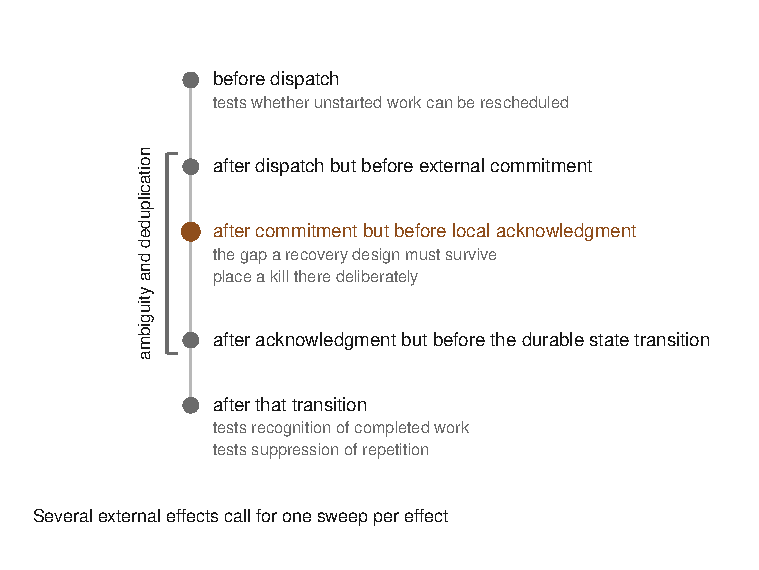
\includegraphics[keepaspectratio,alt={Five lifecycle kill points test recovery from unstarted work through ambiguous commitment gaps to durable completion, including recognition and suppression of repeated external effects.}]{figures/ch09-kill-points.pdf}}
\caption{Five lifecycle kill points test recovery from unstarted work through ambiguous commitment gaps to durable completion, including recognition and suppression of repeated external effects.}
\end{figure}

Each external effect requires a deliberate kill between external commitment and local acknowledgment.

Calls that can hang or return partially add another fault class. Interrupt the connection, inject a retryable response, delay the response beyond the worker heartbeat, and deliver a late response after the retry has begun. The runtime must distinguish a request known not to have executed from one whose status is uncertain. Treating both as ordinary retryable failures converts transport ambiguity into duplicated effects.

Redeployment adds versioned state to the protocol. Kill or replace a worker while a run remains active, then resume it with patched code. The event schema, serialized state, and deterministic replay path may each cross a compatibility boundary. A restart that succeeds with the same binary does not test this case. The configuration record should therefore identify both the pre-fault version and the recovery version.

History growth is another boundary condition. A short demonstration may avoid replay costs, rollover behavior, and compaction defects that appear only after many events. Run beyond the runtime's history rollover or compaction threshold and inject faults on both sides of that boundary.

Compaction replaces detailed working history with a condensed representation so the run remains within its history or context budget. The companion pattern on bounding replay history addresses the architectural response. The experiment determines whether the current boundary behaves as intended.

The fault menu should ultimately come from observed production failures rather than from what the harness can inject conveniently. Worker kills are reproducible and severe, but they do not cover slow storage, stale leases, delayed acknowledgments, partial network partitions, quota errors, or malformed persisted state.

The companion catalog's realistic-fault-menu pattern develops the fuller construction method. The narrower requirement here is to publish the menu so readers can see which failures the recovery claim includes and which it excludes.

\section{Keep the result attached to its envelope}\label{keep-the-result-attached-to-its-envelope}

My kill demonstration, a \textbf{local artifact}, illustrates the protocol without extending the literature evidence. In one run, the worker was killed during an activity after a retryable fault had already been injected. The recovered execution passed all 13 invariant checks. The interrupted activity resumed after a heartbeat-timeout retry, reused a cached result, and produced output identical to the clean reference by content hash.

Thirteen of thirteen is a satisfying result, but it describes one kill placement under one configuration.

I can conclude that the running system exhibited the specified invariants in that trial. I cannot conclude that the engine is generally fault tolerant, that another activity would recover through the same path, or that a different software version would preserve the result. Vogel et al.~(2024) justify that restraint: recovery comparisons changed when configuration and recurring faults were measured directly.

\Needspace{5\baselineskip}

My publish-gate protocol, also a \textbf{local artifact}, defines a broader intended experiment. Its first gate injects a failure in continuous integration at a randomized kill point. The fault matrix includes:

\begin{itemize}
\tightlist
\item
  a kill during a model call;
\item
  a kill inside the execute-then-log gap;
\item
  redeployment with patched code while a run remains active; and
\item
  execution beyond three times the history-rollover threshold.
\end{itemize}

Randomization broadens the sampled placement. It does not replace a fixed sweep across named high-risk intervals.

These artifacts support no comparison among workflow engines. I never ran the comparison sweep, and the non-naive adapters remain specification stubs. There are therefore no author-generated comparative measurements to report. An interface diagram containing several adapters can resemble an experiment even when no workload has passed through them.

\Needspace{5\baselineskip}

Every published result should carry the configuration that produced it. Record:

\begin{itemize}
\tightlist
\item
  runtime and engine versions;
\item
  deployment topology;
\item
  persistence settings;
\item
  checkpoint interval;
\item
  retry policy;
\item
  heartbeat and timeout values;
\item
  resource limits;
\item
  workload shape and concurrency;
\item
  input rate;
\item
  external-service behavior;
\item
  fault-injector version;
\item
  kill-point definition; and
\item
  metric definitions.
\end{itemize}

Preserve the typed trace, or an appropriately redacted derivative, so another investigator can reconstruct the event order. Without this envelope, a recovery number is difficult to interpret and cannot be reproduced closely.

Results also age as the stack changes. A new scheduler, storage client, default timeout, or checkpoint implementation can alter fault detection and state restoration without changing the architecture diagram. A passing experiment establishes behavior only inside the tested envelope. Repeat it after changes that affect persistence, concurrency, retries, version compatibility, external calls, or resource allocation.

Correctness, reliability, and performance should remain separate in the report. The absence of duplicate effects and missing state is a correctness result for a particular trial. The frequency with which those properties hold across injections is a reliability measurement. Recovery time, latency, and throughput are performance measurements.

Resource use and additional model calls belong to cost. An operator's ability to understand the failure and initiate recovery safely belongs to usability. One combined recovery score conceals which property failed.

A recovery system may also need to withhold action when it cannot classify a failure safely. The companion pattern on diagnosing before gating recovery addresses that policy. Another companion pattern asks whether recovery remains invisible to downstream observers except as monotonic progress. Neither property follows from a successful restart, so I exclude both from the basic pass criterion unless the system claims them explicitly.

\section{A protocol for trusting recovery}\label{a-protocol-for-trusting-recovery}

Before accepting a recovery claim about an agent runtime, I look for two linked artifacts.

The first is a durably persisted typed event stream that distinguishes model calls, tool dispatch and completion, environment changes, external commitments, and state transitions. I begin with the shared OpenTelemetry GenAI conventions, then add explicit state, branch, persistence, and effect fields where the workload requires them. Every agent action identifies its owner, and every tool call can be joined to the reasoning step and session that authorized it.

The second artifact is a fault-injection result produced under representative load. I run a clean control, kill a worker from inside an active step, and place at least one kill between an external effect and its durable completion record. I repeat injections within continuing runs and across independent runs because the first restart does not characterize later recovery.

The harness must confirm that the intended kill occurred, observe recovery without supplying recovery state, and exercise a naive negative control expected to duplicate effects.

\Needspace{5\baselineskip}

I measure recovery time between declared application events rather than between process death and process restart. I retain:

\begin{itemize}
\tightlist
\item
  post-recovery throughput and latency;
\item
  invariant outcomes;
\item
  duplicate and missing effects;
\item
  recovery behavior by failure ordinal; and
\item
  output or state equivalence against the clean control.
\end{itemize}

When exact equivalence is impossible, I state which properties were constrained and which outputs remain nondeterministic. A pass means only that the runtime met those conditions in the tested trials.

The fault menu and complete configuration remain attached to the result. Together they define the envelope within which the claim is valid and provide the basis for repeating the experiment after a version or deployment change. A reader should be able to determine which intervals were struck, which faults were omitted, how behavior changed across recurring failures, and which measurements separated correctness from reliability, performance, and cost.

This protocol does not establish that an engine is universally reliable. It supports a narrower and more useful statement:

\begin{quote}
Under a recorded workload and configuration, with specified faults injected at specified boundaries, the runtime recovered with measured behavior and preserved the named invariants.
\end{quote}

That claim can be challenged, repeated, and revised when the system changes.

A trace detailed enough to replay is also the artifact a person reads when recovery fails. Even a complete trace, however, does not establish which action caused the failure or how a person can defend that attribution.

\section*{Sources and evidence}

\textbf{Make every run a structured, replayable trace}

\begin{itemize}
\tightlist
\item
  Directional evidence: Shepherd runtime substrate (Yu et al.~2026, arXiv:2605.10913); companion material named in the same synthesis without a paper identifier: OpenTelemetry GenAI conventions (CNCF 2025).
\item
  Directional evidence: AgentSight eBPF observability (Zheng et al.~2025, arXiv:2508.02736).
\item
  Directional evidence: Chan, A., et al.~(2024), ``Visibility into AI Agents,'' ACM FAccT 2024, arXiv:2401.13138.
\end{itemize}

\textbf{Benchmark recovery with fault injection}

\begin{itemize}
\tightlist
\item
  Strong evidence: Vogel et al.~(2024), ``A Comprehensive Benchmarking Analysis of Fault Recovery in Stream Processing Frameworks,'' arXiv:2404.06203 (JSS line).
\end{itemize}

Author-system cases are narrative illustration, not evidence. The kill demonstration and publish-gate protocol are local artifacts.


\chapter{Human-auditable failure analysis and taxonomy development}
\label{ch10-human-auditable-failure-analysis-taxonomy}
In a peer-reviewed study, Zhang et al.~(\href{https://arxiv.org/abs/2505.00212}{2025}) collected expert-annotated failure logs from 127 multi-agent systems, in which several model-driven workers passed work among one another. They then gave the attribution task to the strongest automated methods they could evaluate. The best method identified the responsible agent in 53.5 percent of cases but found the decisive step in only 14.2 percent. Some methods performed below random.

The logs already existed before the attribution problem was posed. Chapter 9 established that recording what happened is necessary, but a complete record does not establish why a run failed. The same trace may support several causal explanations. One worker may introduce a planning error, another may act reasonably on corrupted state, and a third may expose the defect when verification finally runs. Assigning responsibility to the last visible error confuses detection with cause.

Attribution is the scarce capability in this sequence. Logging preserves evidence. Attribution claims that one action materially changed the run's prospects. That claim determines what engineers instrument, which component they repair, whether a benchmark case remains valid, and sometimes who is held accountable. With weak attribution, a complete trace can become a precise record attached to the wrong explanation.

Three practices follow. I derive the initial failure taxonomy from traces produced by the system I operate. I keep a person responsible for consequential causal assignments. I structure the trace so that person can inspect and defend the evidence. Automation can organize and extend the work after those conditions exist. It should not be assumed to create them.

\section{Build the taxonomy from the failures you can inspect}\label{build-the-taxonomy-from-the-failures-you-can-inspect}

The protocol in this section has limited evidentiary support. Its basis is one directional observational study and one practitioner-authored method. Neither is a controlled result showing that the procedure improves an agent system. I still use it because it provides an auditable process for turning local traces into measurement categories. The method comes from Orosz and Husain (\href{https://newsletter.pragmaticengineer.com/p/evals}{2025}), and their recommendation to begin with at least one hundred traces is an unmeasured protocol choice.

I begin with traces from the system and workload I operate. The sample should vary across task type, outcome, model version, repository area, duration, tool use, and any operating condition likely to alter the path through the system. Apparent successes also belong in the sample when verification was skipped or the result depended on an unexplained retry. Excluding them would define failure as only what the current evaluator already detects, preserving the blind spot the review is meant to uncover.

For each trace, I read from the initial request through the terminal state and take open-ended notes. The primary annotation identifies the first upstream failure that materially changed the available path to success. It does not enumerate every later symptom.

A run may begin with an incorrect plan, edit the wrong module, execute a test from the wrong directory, and then misinterpret the failure. Those are four visible defects. If the plan directed all later work toward the wrong module, the planning error is the first upstream failure.

This rule follows the causal structure of an agent run. State moves from one step to the next through messages, files, tool outputs, summaries, and control decisions. An early error changes the evidence and options available downstream. Later actions may therefore be locally reasonable while remaining globally ineffective. Counting every symptom as a separate failure overweights long runs and systems that continue operating after their prospects have already collapsed.

The first-upstream rule also introduces a counterfactual check:

\begin{quote}
If this step had been correct while the preceding record remained unchanged, could the later failure still have occurred through the observed path?
\end{quote}

A clear no makes the step a plausible causal boundary. A yes suggests that the annotation identifies a symptom, or that the trace does not expose enough state to decide. In the latter case, I preserve the uncertainty and leave the causal assignment unresolved.

\begin{figure}[htbp]
\centering
\pandocbounded{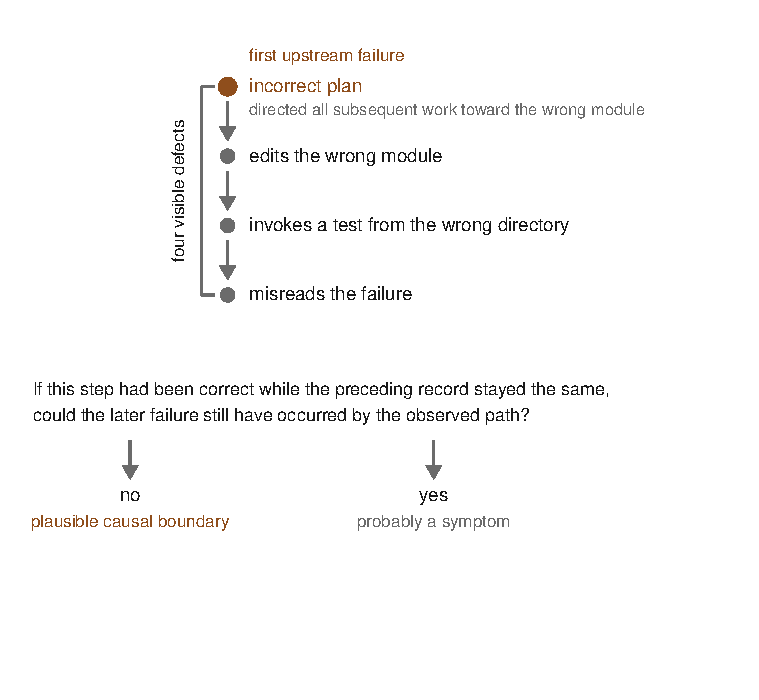
\includegraphics[keepaspectratio,alt={A planning error is the first upstream failure linking four visible defects, while a counterfactual test distinguishes a plausible causal boundary from a symptom.}]{figures/ch10-first-upstream-failure.pdf}}
\caption{A planning error is the first upstream failure linking four visible defects, while a counterfactual test distinguishes a plausible causal boundary from a symptom.}
\end{figure}

The counterfactual holds the preceding record fixed and asks whether the observed path could still have produced the later failure.

After the open review, I cluster the notes into roughly five to ten themes. The categories should describe failures that require different measurement or investigation surfaces. Planning, retrieval, execution, tool use, self-diagnosis, verification, and environment handling may emerge, but I do not impose them before reading the traces. A local pipeline may instead concentrate failures around identity propagation, stale workspace state, permission boundaries, retry ordering, or task ambiguity.

Phase labels are useful because they narrow the evidence required for diagnosis. A planning failure asks whether the system represented the goal, constraints, and dependencies before acting. An execution failure asks whether a valid plan became the intended commands and edits. A self-diagnosis failure asks whether the system interpreted the resulting state correctly. Combining all three under ``reasoning failure'' produces a broad count with little guidance about which part of the trace needs repair.

Generic metric packages often begin with categories that are convenient for the evaluator. They count tool errors because tool errors are easy to parse, or grade final answers because final answers are easy to present to a judge. The resulting dashboard may be internally consistent while missing the upstream decisions that generated those events. A taxonomy derived from traces begins with the failure process and asks only afterward which measurements can represent it.

Published phase-aligned classifications provide useful comparisons. Lu et al.~(\href{https://arxiv.org/abs/2508.13143}{2025}) classified failures by phase across 34 programmable tasks executed by off-the-shelf frameworks operating near 50 percent completion.

Their distribution does not establish base rates for frontier coding agents. It describes the tasks, systems, permissions, and operating point in that study. A production repository with different tools, review gates, task durations, and authority boundaries may concentrate failures elsewhere.

I encountered this mismatch in my own trial-annotation pipeline for experimental agent runs. An early taxonomy omitted failure modes that dominated the project's traces even though public taxonomies covered related categories. The third revision grew from annotation of the local corpus and separated failures along more dimensions. This is narrative illustration only. It does not establish that the resulting taxonomy is complete, and the published export cannot independently reproduce the category counts because its manifest contains no annotations.

The unit of analysis is a complete case. I keep the request, relevant starting state, trace, terminal outcome, verification result, and annotation together. When several retries belong to one attempt, I preserve their order and identities so that a later successful retry does not erase the original failure. When the system forks work, I retain the parent-child relationship. Otherwise an error imported from another branch may appear to originate where it was first observed.

Category boundaries will blur in long, multi-phase work. A retrieval failure can induce a bad plan, while an environment defect can make correct execution resemble faulty reasoning. I allow multiple descriptive tags when they preserve useful context, but retain one first-upstream assignment for frequency analysis. This avoids pretending that causation is always singular while keeping the primary count interpretable.

Reviewer disagreement is evidence about the taxonomy. If two qualified reviewers repeatedly divide the same cases between planning and retrieval, the definitions may depend on state the trace does not expose. If they agree about the events but disagree about the counterfactual, the causal rule needs a sharper boundary. I revise the definitions and preserve the original annotations so the change remains visible.

The initial review of roughly one hundred traces is intentionally laborious. Reading them end to end discovers categories, tests whether the recorded evidence can support those categories, and identifies distinctions that require domain expertise. It cannot estimate a stable low-frequency failure rate with the precision that a larger sample and a \textbf{power analysis} would require. A frequency calculated from one run per task also inherits the run-to-run variation described in Chapter 1, so two nearby categories may reverse order under repetition.

The output of the initial pass is a defensible measurement vocabulary and a labeled seed corpus. Estimating the system's failure distribution requires a separate sampling design.

Once the categories stabilize, scale-out returns to Chapter 5. I validate an LLM-as-judge on a held-out, expert-labeled, stratified sample under the same rubric. I then use it to extend labels only within the operating range supported by its measured errors. The validation belongs to the category definitions in force when it ran. Revising a definition invalidates the agreement estimate for that category.

Human review remains concentrated on new categories, ambiguous cases, consequential failures, and strata in which the automated judge performs poorly. Applying a prebuilt judge before the manual pass would automate someone else's taxonomy rather than discover the failures produced by the local system.

Frequency informs priority without determining it. I count first-upstream assignments by phase and category, examine their uncertainty, and compare their prevalence with the cost of each failure. A frequent, recoverable tool error may deserve less attention than a rare attribution error that invalidates an evaluation. The distribution shows where failures concentrate. Engineering judgment still decides which failures are worth repairing.

Several narrower methods remain in the companion catalog. Constraint-violation logs can localize failure when a task has explicit invariants. Trajectory canonicalization can support structural comparisons across runs. Another entry recommends detecting environment errors before execution because they can consume disproportionate effort. These techniques may sharpen a local taxonomy, but none removes the need to discover which categories the operated system actually produces.

\section{Keep causal assignment under human control}\label{keep-causal-assignment-under-human-control}

Attribution becomes consequential when it changes what happens next. An engineer may rewrite a prompt, repair a tool adapter, remove a benchmark task, retrain a model, or revise an incident report based on the assigned cause. The same label may also affect accountability when different people or services own different parts of the run. In those cases, an automated guess is not a harmless summary.

I separate triage from verdict. Triage ranks cases or candidate steps for investigation. A verdict identifies the responsible action and decisive step, supported by enough evidence that another reviewer can challenge the assignment. Automation can make triage cheaper even when its error rate makes it unsuitable for verdicts.

The opening result shows the current limit. An agent-level accuracy of 53.5 percent leaves nearly half of responsible-agent assignments wrong. A step-level accuracy of 14.2 percent misses the point at which most failures became decisive.

Those figures do not establish a general ceiling for automated attribution. They come from one annotated dataset of multi-agent failures. Single-agent coding traces may be easier, other workloads may be harder, and later methods may improve substantially. The percentages should not be converted into a staffing ratio or a universal automation threshold.

Ma et al.~(\href{https://arxiv.org/abs/2509.08682}{2025}) later reached 36.2 percent step-level accuracy on the same benchmark family, compared with less than 15 percent for prior methods. Counterfactually validated fixes derived from that analysis increased task success by an average of 22.4 percent, although the source does not state whether that gain is absolute or relative. The result suggests that causal structure can narrow the search more effectively than an undifferentiated reading of the transcript. The method still assigned most decisive steps incorrectly.

The fixes were evaluated on the benchmarks that defined the attribution task, and the method required a bespoke causal-discovery algorithm for interaction data whose behavior changes over time. That makes it useful as a candidate generator for a reviewer. It does not justify silently storing its assignment as the postmortem cause.

\Needspace{5\baselineskip}

A human verdict needs a reconstructable chain. I ask:

\begin{itemize}
\tightlist
\item
  Which state changed?
\item
  Which action changed it?
\item
  Which later components consumed that state?
\item
  Which observation eventually exposed the damage?
\end{itemize}

The record must distinguish the actor that introduced the defect from the actor that detected it. It must also distinguish a component that merely propagated invalid state from one that had both the information and the responsibility to reject it.

Consider a run in which a planner selects an obsolete interface, a coding worker implements it faithfully, and a verifier reports an integration failure. The verifier owns the detection. The planner is the first candidate for causal responsibility, provided the current interface was available in the planner's evidence and no later gate explicitly owned the currency check. If the repository index supplied stale documentation, responsibility may move again.

The trace cannot resolve those alternatives unless it records what each step received and what obligation each step owned.

\Needspace{5\baselineskip}

I therefore represent attribution as a structured claim. It records:

\begin{itemize}
\tightlist
\item
  the first upstream action;
\item
  the state transition that action caused;
\item
  the downstream dependency that carried the error;
\item
  the evidence supporting the assignment;
\item
  plausible alternatives considered;
\item
  the reviewer's confidence; and
\item
  the reviewer's identity.
\end{itemize}

This structure does not make the judgment objective. It makes visible where judgment entered. A postmortem that names a ``root cause'' without identifying the state transition behind it is a summary rather than an attribution.

Counterfactual reasoning tests an attribution without proving it. I ask whether replacing the candidate action with a correct one, while holding earlier state fixed, would have prevented the observed failure path. Several steps may satisfy that condition because later checks could also have recovered the run.

Under the taxonomy used here, the decisive step is the earliest point at which the relevant error entered the run or an owned opportunity to stop it was irretrievably missed.

That definition requires an explicit ownership model. A verifier that was never assigned responsibility for checking interface currency should not inherit responsibility merely because it could have caught the error. A release gate whose declared contract includes that check does own a meaningful missed intervention. Postmortems become arbitrary when they infer obligations from hindsight rather than from the contracts active during the run.

Retries complicate attribution because the world may change between attempts. A failed attempt can alter files, caches, rate limits, conversation state, or the evidence presented to the next attempt. A successful retry may depend on those changes, while a later failure may be responding to damage introduced earlier. I preserve attempt identity and state boundaries so reviewers can distinguish a repeated decision from a decision made in a changed environment.

Concurrency creates another ambiguity. Two workers may read the same starting state, make individually valid changes, and conflict only when their outputs merge. Neither branch necessarily contains a unilateral defect. Depending on the violated contract, the failure may belong to the coordination rule, merge order, or missing conflict check. A transcript sorted by completion time can make the worker whose result arrived last appear responsible for a conflict it did not cause.

Before assigning fault to an agent, I rule out the evaluator and execution environment. A broken dependency, stale fixture, permission mismatch, nondeterministic test, or malformed task can make a correct action appear defective. Differential testing runs the same candidate under a controlled change in agent, harness, or environment and asks whether the failure follows the candidate. The companion catalog treats this as a separate diagnostic control because attribution without apparatus checks can turn measurement error into a model failure.

Human control does not require every reviewer to read every trace from the beginning. Automated systems can rank likely decisive steps, group similar incidents, retrieve related cases, prefill observed events, and flag assignments inconsistent with the recorded state transitions. The reviewer remains responsible for accepting, revising, or abstaining. The stored record distinguishes the automated proposal from the signed attribution.

I used the same authority boundary in my internal benchmark-curation process, which determined whether generated software tasks were sound enough to evaluate. Candidate decisions retained an explicit provisional label until a project lead approved them. The pipeline could assemble evidence and run checks, but it could not finalize whether a defect belonged to the task or the evaluated system. This methodology example supplies no accuracy evidence.

The review threshold should follow consequence. A low-stakes transient failure may retain an automated tentative label for aggregate triage. A failure that changes remediation, removes an evaluation item, alters a reported result, or assigns organizational responsibility requires a named human decision.

When the evidence cannot distinguish among plausible causes, the correct verdict is unresolved. The record should state which missing observation would have separated them.

Aggregating several automated readers does not by itself make attribution reliable. The companion catalog describes independent attribution judges as an aside, but agreement among several weak or dependent readers does not establish causation. It also treats consistency across repeated runs as a risk signal. Both may help decide where a person looks first. Neither should determine what that person must conclude.

Repeated local categories can eventually expose a structural defect. When the same failure class survives prompt patches and model upgrades, the remedy is likely architectural, and Chapter 17 develops that redesign question. This chapter stops at diagnosis because recurrence alone does not establish the correct intervention.

\section{Design the record for a skeptical reader}\label{design-the-record-for-a-skeptical-reader}

Deshpande et al.~(\href{https://arxiv.org/abs/2505.08638}{2025}) reported that the strongest evaluated long-context model correctly localized issues in 11 percent of 148 expert-annotated traces. The traces were benchmark-derived but ecologically valid and more complex than short synthetic sequences designed to isolate one error. Reasoning, tool calls, outputs, retries, and state changes appeared in the same record. A large context window could contain the transcript, but containment did not make the decisive event legible.

\begin{figure}[htbp]
\centering
\pandocbounded{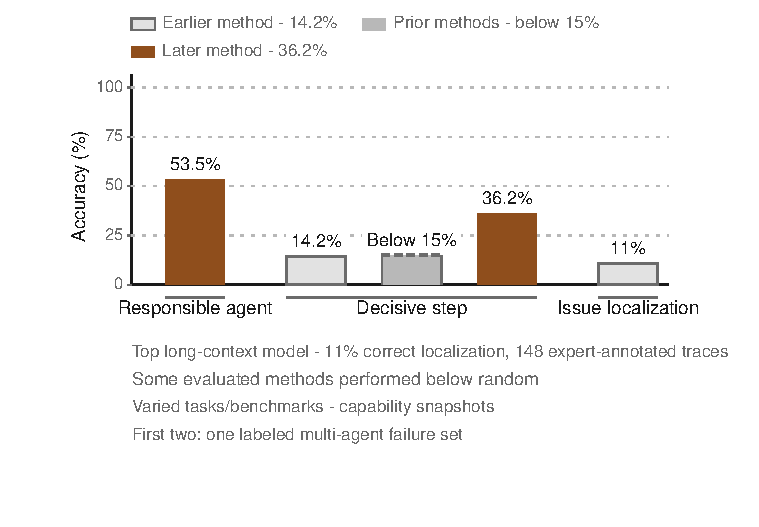
\includegraphics[keepaspectratio,alt={Responsible-agent attribution is 53.5\%; decisive-step attribution is 14.2\% earlier, below 15\% for prior methods, and 36.2\% later; the top long-context model localizes 11\% of 148 traces, and some methods underperform random.}]{figures/ch10-attribution-accuracy.pdf}}
\caption{Responsible-agent attribution is 53.5\%; decisive-step attribution is 14.2\% earlier, below 15\% for prior methods, and 36.2\% later; the top long-context model localizes 11\% of 148 traces, and some methods underperform random.}
\end{figure}

These results span different tasks and benchmarks. The first two use one annotated dataset of multi-agent failures. They are capability snapshots, not a general automation ceiling.

The model scores will change as trace readers improve, and the benchmark cannot establish performance for every production workload. The more durable implication comes from the structure of the task. A record built for human audit should expose the units a causal investigation requires. Raw chronological text forces every reader, human or model, to reconstruct those units before diagnosis begins.

Chapter 9's typed event stream supported replay and recovery. Human audit adds a different requirement. A reviewer must be able to follow step boundaries, decisions, inputs, state transitions, retries, and outcomes without inferring their identities from prose. The same event stream can support both purposes when its schema records semantic boundaries. Timestamps on messages alone do not preserve them.

\Needspace{5\baselineskip}

At minimum, I retain:

\begin{itemize}
\tightlist
\item
  a run identifier;
\item
  the task identity;
\item
  model and configuration versions;
\item
  an initial-state reference; and
\item
  ordered step identifiers.
\end{itemize}

\Needspace{5\baselineskip}

Each step records:

\begin{itemize}
\tightlist
\item
  the actor;
\item
  input references;
\item
  the decision or intended action;
\item
  the tool request;
\item
  the tool response;
\item
  the resulting state reference;
\item
  the verification outcome; and
\item
  the terminal status.
\end{itemize}

Retries identify the attempt they repeat and the reason the controller authorized another attempt. Forks and joins preserve parentage and ordering constraints.

A tool response, file digest, exit status, or test result is an observation. A model statement that the response means a dependency is missing is an interpretation. Storing both under a generic message field encourages later readers to treat the interpretation as though it came from the environment. Typed events allow the reviewer to compare the claim with the observation on which it rests.

Decision records need enough input to reevaluate the choice. A label such as ``selected tool A'' records the outcome but omits the alternatives, constraints, and evidence available at the time. I preserve the relevant input references, selected action, rejected alternatives when the system represented them, and the rule or model version that made the selection.

Replay means re-running or reevaluating a decision against the same recorded inputs. Asking a model to invent a retrospective rationale is a different operation.

Some inputs cannot be stored in full. Repository snapshots, retrieved documents, and tool outputs may be large, sensitive, or mutable. The trace can instead retain content-addressed references, access-controlled snapshots, or a precise query together with the identities of the returned items. A pointer to ``current repository state'' is insufficient because the state will change before review. The preservation policy must balance reproducibility with confidentiality, storage cost, and retention obligations.

Step boundaries should correspond to ownership and state transitions visible to the control plane. One step containing plan generation, three tool calls, an edit, and verification is too coarse for attribution. Recording every token or streaming fragment produces the opposite failure: thousands of events without a meaningful decision boundary.

I use the smallest unit in which one actor receives a defined input and produces an action or state transition consumed by another component.

\Needspace{5\baselineskip}

Tool-call records need more than a name and final output. They should include:

\begin{itemize}
\tightlist
\item
  normalized arguments;
\item
  execution-environment identity;
\item
  start and completion status;
\item
  timeout or cancellation state;
\item
  a summary of side effects; and
\item
  links to resulting artifacts.
\end{itemize}

A command can return a nonzero exit status after partially changing the environment. Recording only the failure status hides files, processes, or external effects inherited by the retry.

Ordering also needs explicit semantics when work overlaps. Wall-clock timestamps help diagnose latency, but clock order does not establish causality across concurrent workers. Parent identifiers, message sequence numbers, versioned state references, and join events show which observations were available to each decision. When two steps race to modify the same artifact, the trace should identify the accepted version and the rule that rejected or merged the other.

Identity must remain stable across resumed work. A display name such as \texttt{coder} may refer to different model versions, sessions, or permission sets. The audit record links the logical role to a particular execution instance, configuration, authority set, and parent run. This lets a reviewer determine whether an outcome changed because of a new decision, a new actor, or state inherited across a restart.

The review interface should support competing explanations. A reviewer should be able to move from an annotated failure to the suspected upstream event, inspect its input state, follow affected descendants, and compare a neighboring successful run. Filtering by actor or event type is useful, but the default view should preserve causal context around each selection. A viewer that hides retries or collapses repeated tool output may improve readability by removing the evidence under dispute.

CodeProbe (\href{https://github.com/sjarmak/codeprobe}{public repository}) publishes complete transcripts and preserves quarantined runs separately. Its successor adds a side-by-side trace browser for audited comparisons. These choices illustrate preservation and review practices. They do not establish that the schema is optimal, and publication alone does not prevent incorrect conclusions.

Quarantined runs are worth preserving because evaluation pipelines often remove timeouts, rate limits, infrastructure failures, and malformed outputs before analysis. Some exclusions are methodologically justified, but deletion prevents a later reviewer from distinguishing an agent failure from an apparatus failure. I retain the raw run, exclusion reason, decision owner, and any replacement attempt. Aggregate reporting can then follow the declared policy without erasing the cases that test it.

Structured traces also improve privacy controls because sensitive fields become identifiable. Credentials, personal data, proprietary source, and private model reasoning may require redaction or restricted access. Blanket retention creates a security liability, while blanket deletion destroys auditability. Field-level policies can restrict access, encrypt retained data, and irreversibly redact secrets. The record should distinguish evidence withheld by policy from evidence the system never captured.

The trace schema must record its own version. Adding a field changes what can be inferred from later runs. Renaming an event can break comparisons with the existing failure corpus. A missing field may mean that the event did not occur, that the recorder omitted it, or that an older schema represented it differently. The decoder and migration logic should distinguish those states explicitly.

Instrumentation can also change the system being observed. Synchronous logging adds latency. Large payloads can alter token budgets, memory use, or rate-limit behavior. Asynchronous emission can reorder records or lose the final buffer during a crash. I measure the overhead, assign a durability requirement to each event class, and record missing events as trace failures. A gap must remain visible in the reconstructed record.

Changing instrumentation between experimental arms also changes the apparatus, which Chapter 1 requires to remain fixed in a paired comparison.

The practitioner evidence for this practice is anecdotal. One organization reported that reviews had consisted of competing opinions until the system began recording decisions, inputs, retries, and outcomes. The resulting structure made failures repeatable and disputes more factual. A second practitioner independently described event-sourced, replayable traces. Both are self-reported accounts. They demonstrate plausible operational use but no controlled improvement or universal schema.

Logging does not repair an agent. It makes causal explanations testable against preserved events and makes repeated failure paths comparable. Repair still requires a separate intervention and an evaluation showing that the intervention changed the intended outcome. This distinction prevents observability work from receiving credit for reliability gains it has only made possible to measure.

The schema should evolve from failed investigations. Common gaps concern the state a worker observed, side effects inherited by a retry, the branch selected at a join, or the evidence behind a decision. I record the unanswered question as an instrumentation defect. The next schema version adds the smallest event or relation that would have answered it. This ties auditability to real investigations and limits speculative completeness.

Trajectory shape can provide an early signal while a run remains active. The companion catalog describes monitoring duration, variance, tool-call count, and other structural changes because failed trajectories may run longer or become more variable. Such a signal can preserve a suspicious run or request earlier review. It cannot identify the cause without the structured events that explain what occurred inside that shape.

\section{Turn failed runs into an operating record}\label{turn-failed-runs-into-an-operating-record}

I begin with the twenty most recent failed runs and read each one from the initial request through the terminal state. My notes remain open-ended, and each case receives one primary assignment: the first upstream failure that materially changed its path to success. I also include apparent successes whose verification was skipped, because an unverified outcome cannot provide clean evidence of success.

This first batch tests the trace as much as the system. It shows whether the record can answer ordinary causal questions before a larger annotation effort depends on it.

I then expand the corpus toward one hundred traces selected across task types, outcomes, model versions, repositories, durations, tools, and operating conditions. I cluster the notes into roughly five to ten failure classes. Their observed frequency helps determine which classes to measure first, while consequence and repair cost determine the final priority.

A named human signs any attribution that changes remediation, accountability, task validity, or the interpretation of an evaluation result. Automated readers may rank the review queue, retrieve related cases, and propose candidate decisive steps. They do not finalize the causal assignment.

The first question the trace cannot answer becomes an instrumentation requirement. I add the missing state reference, event boundary, identity, ordering relation, or outcome field, then preserve the new schema version with later runs. Failed analysis therefore becomes evidence about the observability system itself.

A completed review should state both what the evidence supports and what remains unresolved.

The failure corpus remains an operating asset after Part III. Chapter 14 uses it to tune compaction policy, because compression should preserve the evidence that prior investigations found decisive.

Part IV turns to the evidence available when the model acts: retrieval, context budgets, and memory. Chapter 11 begins by measuring repository retrieval, the first step in deciding which parts of a codebase enter that evidence.

\section*{Sources and evidence}

The evidence grouping on each entry below comes from its catalog record. Author-system cases in this chapter are narrative illustration and are not part of the evidence base.

\textbf{Derive the failure taxonomy from your own traces}

\begin{itemize}
\tightlist
\item
  Directional evidence: Lu, R., Li, Y., Huo, Y. (2025), ``Exploring Autonomous Agents: A Closer Look at Why They Fail When Completing Tasks,'' arXiv:2508.13143. (Phase-aligned classification; \textasciitilde50\% completion base rate on 34 programmable tasks with off-the-shelf frameworks; not an estimate for production repositories.)
\item
  Directional evidence: ``A pragmatic guide to LLM evals for devs'', Gergely Orosz with Hamel Husain, Pragmatic Engineer newsletter, 2025-12-02, \url{https://newsletter.pragmaticengineer.com/p/evals}. (Open coding on 100+ traces, first upstream failure, axial coding into 5-10 themes, prioritize by frequency.)
\end{itemize}

\textbf{Keep humans in failure attribution}

\begin{itemize}
\tightlist
\item
  Strong evidence: Zhang, S., et al.~(2025), ``Which Agent Causes Task Failures and When? On Automated Failure Attribution of LLM Multi-Agent Systems,'' ICML 2025, arXiv:2505.00212. (Who\&When: expert-annotated failure logs from 127 multi-agent systems; 53.5\% agent-level and 14.2\% step-level for the best automated method; some methods below random.)
\item
  Directional evidence: Ma, G., et al.~(2025), ``Automatic Failure Attribution and Critical Step Prediction Method for Multi-Agent Systems Based on Causal Inference,'' arXiv:2509.08682 (CDC-MAS). (36.2\% step-level against under 15\% for prior methods; counterfactually validated fixes worth an average 22.4\% task success.)
\end{itemize}

\textbf{Design traces for human audit}

\begin{itemize}
\tightlist
\item
  Strong evidence: Deshpande, D., et al.~(2025), ``TRAIL: Trace Reasoning and Agentic Issue Localization,'' Patronus AI, arXiv:2505.08638. (Best evaluated model localized issues in 11\% of 148 expert-annotated traces; a 2025 capability snapshot.)
\item
  Corroborating case: ``What actually broke when we put AI agents into real production workflows'', /u/saurabhjain1592, r/LLMDevs, 2026-01-08.
\end{itemize}

\textbf{Author-system illustration cited inline}

\begin{itemize}
\tightlist
\item
  Not an evidence item: CodeProbe, the author's task-mining evaluation tool, \href{https://github.com/sjarmak/codeprobe}{public repository}. Named inline for the published transcripts and quarantined runs described above, which are narrative illustration.
\end{itemize}


\part{Context engineering: retrieval, budgets, and memory}

\chapter{Measuring and designing repository retrieval}\label{measuring-and-designing-repository-retrieval}

In my own benchmark built from tasks across 73 repositories, two instruments disagreed about the same retrieval tool. \href{mailto:Precision@10}{\nolinkurl{Precision@10}}, the proportion of the first ten results judged relevant, rose from 0.095 to 0.313. \textbf{\href{mailto:Recall@k}{\nolinkurl{Recall@k}}}, the fraction of judged needed items found among the first \(k\) results, rose at \(k=10\) from 0.120 to 0.272. The fraction of tasks for which the needed file appeared rose from 0.33 to 0.56. The paired end-to-end reward across 370 tasks moved by only +0.0349, with a bootstrap 95\% confidence interval of {[}+0.0130, +0.0579{]}, n = 370.

This bootstrap treated all 370 task-level deltas as independent observations. The tasks were drawn from 73 repositories and grouped into 20 suites, and the resampling reflected neither structure. The reported interval therefore likely understates the uncertainty and should not be read as a bound on it.

Chapter 1's rule about choosing the resampling unit applies directly here, but promoting the unit to the repository or to the suite is not sufficient on its own. Repositories and suites are two groupings over the same tasks. Whether they are nested or crossed determines whether one clustered unit is adequate or the analysis needs a hierarchical or multiway resampling procedure.

The retrieval measurements showed that the tool had become substantially better at putting relevant repository evidence in front of the agent. The final score showed that the system as a whole had changed little. Each scoring procedure estimated a different event.

This disagreement changed the engineering question. If I had kept only the final reward, I would have treated the retriever as a weak intervention and looked elsewhere. The stage measurements showed that retrieval had improved while much of the added evidence failed to become correct edits. The next investigation therefore belonged downstream, in context assembly, evidence use, generation, or verification.

The reverse pattern would have required a different explanation. An end-to-end gain without a retrieval gain could have come from a model change, a prompt difference, or some other uncontrolled part of the path.

Repository retrieval sits inside a causal chain. A task becomes one or more queries. Each query searches an index. Ranked results enter a context budget. A model interprets that context, and an execution and verification process turns the model's output into a scored result. A pass rate records the state at the end of the chain, and it cannot identify which transition produced that state.

\section{Score retrieval and generation separately}\label{score-retrieval-and-generation-separately}

Chapter 2 used ablations to isolate a component by removing it while holding the surrounding system fixed. Stage-level scoring applies the same attribution discipline within a run. I measure whether the retriever surfaced the evidence the task required, where that evidence appeared, whether it survived the context cutoff, and whether the generator used it. I report those measurements beside the final completion score, because each describes a different condition for success.

The first condition is availability. The relevant file, symbol, documentation block, or prior decision must exist in the searchable corpus and in its index. A retriever cannot return a file omitted by an indexing rule, a generated source tree excluded as noise, or a recently changed document still waiting for an asynchronous update. Treating these as ranking failures sends the investigation toward query tuning when the actual defect is corpus coverage or freshness.

The second condition is retrieval. Given an indexed target, the query must bring it into the returned set. The third is placement, because a relevant item can appear too low in the list to survive a fixed depth or token budget.

The fourth condition is contextual sufficiency. A method signature may be relevant but insufficient when the implementation, callers, or type definition determine the edit. The fifth is use. The model may receive adequate evidence and still ignore it, misread it, or produce an edit that fails for an unrelated reason.

An end-to-end failure is compatible with failure at any one of these conditions, and also with several at once. A tool can find the right method at position twelve, the context builder can keep ten results, and the generator can then invent an interface from the remaining snippets. The final failure does not reveal whether query formation, ranking, truncation, or generation should change. The trace does, but only when the evaluation has recorded the boundaries between those stages.

\begin{figure}
\centering
\pandocbounded{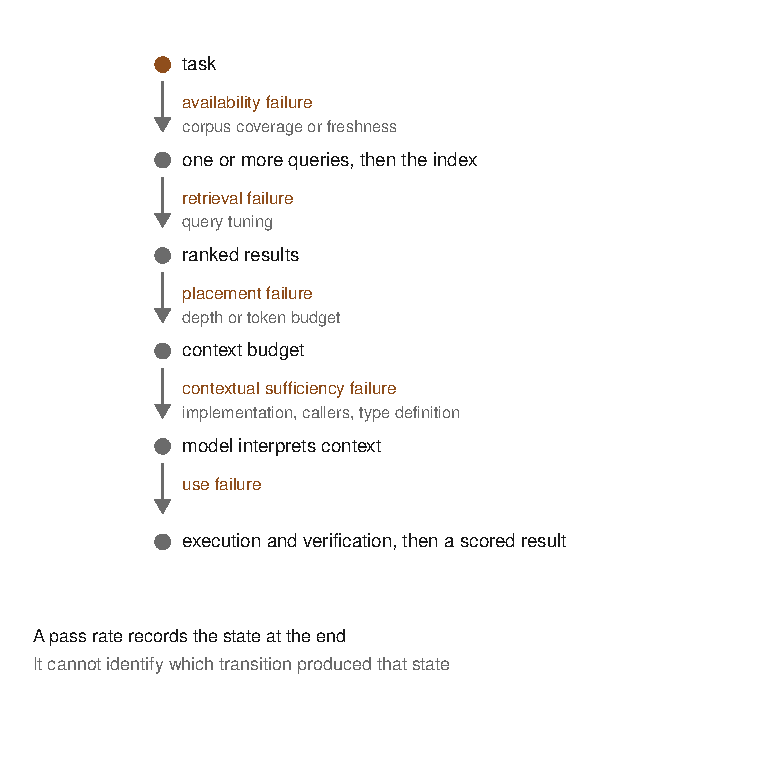
\includegraphics[keepaspectratio,alt={The retrieval chain separates availability, retrieval, placement, contextual sufficiency, and use failures across the transitions from task formulation to scored execution and verification.}]{figures/ch11-retrieval-chain.pdf}}
\caption{The retrieval chain separates availability, retrieval, placement, contextual sufficiency, and use failures across the transitions from task formulation to scored execution and verification.}
\end{figure}

Pass rate captures only the final state, so it cannot reveal which transition failed or which governing condition caused the result.

The same ambiguity appears when a task passes. A generator may solve a familiar edit from model knowledge while the retriever returns irrelevant material. A broad retriever may place the answer somewhere in a large dump that exceeds the model's useful attention and still receive credit, because the final edit happens to work. Chapter 6's return-everything case reached recall 1.0 by construction. Correctness at the end of the run does not certify the evidence path that preceded it.

I therefore keep a per-task record with at least four fields: the identifiers of the judged relevant items, their positions in the returned list, the subset that entered model context, and the final task outcome. When the system exposes citations, tool references, or another reliable evidence-use signal, I add which items the generator actually used. A copy of the retrieved text in the prompt establishes exposure alone.

Repository-level code completion research supplies a clean example of this decomposition. RepoBench, from Liu et al.~(\href{https://arxiv.org/abs/2306.03091}{2023}), evaluates retrieval, completion with supplied context, and the combined pipeline as separable conditions. This design distinguishes a system that cannot retrieve the useful cross-file context from one that receives that context and cannot complete the code. A better ranker addresses the first failure and leaves the second untouched.

Memory evaluations expose a similar split through different measurements. MemConflict, from Tao et al.~(\href{https://arxiv.org/abs/2605.20926}{2026}), combined final-answer scoring with observations of whether the required memory was absent, ranked too low, retrieved but unused, or used incorrectly. Its evaluated systems answered correctly while the best reported conflict-recognition score across them reached only 0.2501. Memory Circuit Analysis, from Mao et al.~(\href{https://arxiv.org/abs/2605.03354}{2026}), reports a stage-level diagnostic that localizes a silent failure to the memory operation responsible for it, because extraction, retention, and retrieval can fail behind fluent responses. These results support stage localization, but their memory workloads do not reproduce all of the constraints of repository-scale software work.

Three newer studies provide directional support for the same measurement shape. SkillEvolBench, from Lei et al.~(\href{https://arxiv.org/abs/2605.24117}{2026}), and EngramaBench, from Acuna (\href{https://arxiv.org/abs/2604.21229}{2026}), examined whether stored or evolved material remained available and useful while also reporting final answers. A cost-and-accuracy study by Wolff and Bennati (\href{https://arxiv.org/abs/2601.07978}{2026}) separated what a memory system retrieves from what the answering model produces. I use those three to establish direction, and not as a numerical basis for a repository retrieval policy.

\subsection{Retrieval metrics}\label{retrieval-metrics}

With one required item, the per-task \href{mailto:Recall@k}{\nolinkurl{Recall@k}} value is binary, because the item is either present or absent. With several required items, it is the fraction found in the first \(k\). The aggregate reports the mean across tasks. When tasks require unequal numbers of items, that mean and the pooled fraction over all required items are different estimands, and the report should name the one it uses. The relevance judgment must also state which items count.

A file-level version counts the needed file, while a chunk-level version can require the specific definition or surrounding block. Those targets answer different questions and must be named.

The \textbf{rank} of a needed item is its position in the ordered results, with position one returned first. An item at position one and an item at position ten both count as retrieved when \(k=10\), although the first consumes less context and is less vulnerable to truncation. A single \href{mailto:Recall@k}{\nolinkurl{Recall@k}} value does not record that difference. When several items are needed, I record each position or a stated aggregate, because one number rarely describes the set.

Retrieval depth is an experimental variable. I sweep \(k\) across a range and plot recall as a function of depth. The \textbf{recall plateau} is the region where that curve flattens. Past it, returning additional items recovers little more required evidence. Choosing \(k\) before inspecting the curve biases every comparison.

A shallow cutoff can make a viable retriever look incapable. A deep cutoff can conceal poor ranking, because a disordered list still contains the target somewhere among its returned items. The plateau does not determine the operating point on its own, since latency, context consumption, and distractors can justify stopping earlier. It shows what recall the ranking can reach and the marginal cost in returned items.

\begin{figure}
\centering
\pandocbounded{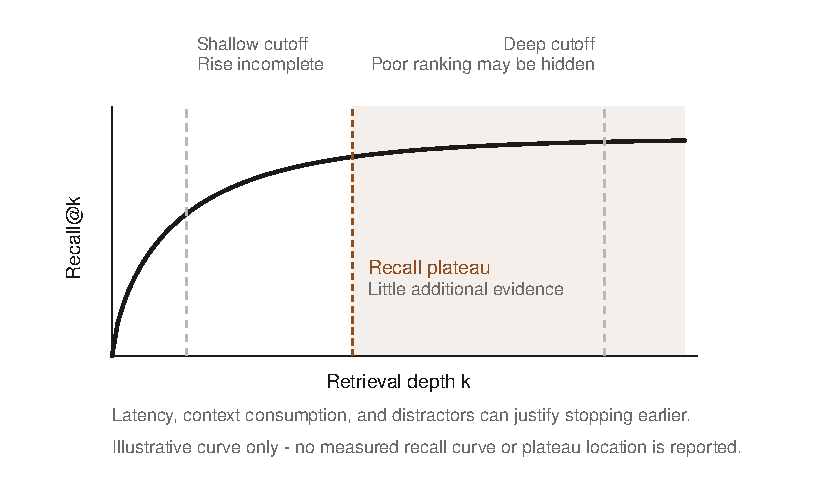
\includegraphics[keepaspectratio,alt={An unmeasured recall curve rises and plateaus with retrieval depth, but a shallow cutoff leaves gains unrealized, a deep cutoff can mask poor ranking, and latency, context use, or distractors may justify stopping earlier.}]{figures/ch11-recall-depth.pdf}}
\caption{An unmeasured recall curve rises and plateaus with retrieval depth, but a shallow cutoff leaves gains unrealized, a deep cutoff can mask poor ranking, and latency, context use, or distractors may justify stopping earlier.}
\end{figure}

Shallow cutoffs understate retrieval capability, while deep cutoffs can hide poor ranking. Latency, context consumption, and distractors may justify stopping before the plateau.

Multiple retrieval channels produce ordered lists whose numeric scores often have different meanings. BM25, a lexical ranking function based on term occurrence and document statistics, can emit values well above one. Cosine similarity for embedding vectors usually occupies a bounded interval. Adding or averaging those raw values gives arbitrary influence to whichever implementation happens to produce larger numbers.

\textbf{Reciprocal-rank fusion} combines lists by position. Each item receives a contribution such as \(1/(c+r)\) from each lane, where \(r\) is its position and \(c\) is a fixed damping constant. The fused order depends on agreement and placement across lists, and it ignores incomparable score scales.

Each of these measurements is incomplete in a different way. A single \href{mailto:Recall@10}{\nolinkurl{Recall@10}} can be useful, but it does not show whether ten sits before or after the plateau. A mean rank does not report the tasks in which the target did not appear at all. Missing items therefore need an explicit convention and a separate recall report. A fused list can improve coverage even when one channel has failed, and that failure is visible only when the original lane results remain available.

Stage-level evaluation requires relevance judgments. In a curated benchmark, maintainers can identify the file, symbol, span, or set of dependencies needed to solve each task. In a production repository, relevance may be plural and conditional. One correct patch may use the interface declaration and a caller. Another may use the implementation and a test. Declaring only one path relevant can penalize an equally valid evidence route.

I build judgments from the task's accepted solution, dependency structure, and expert review when the evaluation warrants that expense. I retain graded labels when an item can be useful without being sufficient. A class declaration may receive a relevance label, for example, while the concrete override receives a sufficiency label for the task. Whichever label schema is used, the record must document what qualified an item and which valid solution paths the annotators considered.

The expense limits where decomposition can be applied. Repository-scale relevance judgments require people who understand both the task and the codebase, and a changing repository can invalidate them. Sampling can control the cost. Annotate a stratified subset, preserve the adjudication record, and use it to diagnose the rest of the evaluation without pretending that unlabeled tasks have measured retrieval quality. A retrieval proxy based only on file overlap with one reference patch is cheaper, and it should be reported as that proxy.

Five terms can help reviewers describe the retrieved context: relevance, sufficiency, isolation, economy, and provenance. Relevance asks whether an item bears on the task. Sufficiency asks whether the returned set contains enough evidence to act correctly. Isolation asks whether the evidence is separated from material likely to mislead the model. Economy measures the context consumed to convey the evidence. Provenance records where the item came from and which version it represents.

This vocabulary comes from a position paper by Vishnyakova (\href{https://arxiv.org/abs/2603.09619}{2026}) and is not a measurement protocol. Each property needs an operational definition tied to the evaluated system before it can enter a score.

Evidence-use measurement is harder than exposure. Model-generated citations can be incomplete or post hoc. Removing one retrieved item and rerunning the task is an ablation, but model variability can change the output for reasons unrelated to that item. Attention weights do not establish causal use.

I therefore combine the available signals and state what each one supports. Exposure logs show what the model received. Citations show what it claimed to use. Controlled removal estimates whether the item changed outcomes across repeated runs.

The decomposition also changes the interpretation of verbose retrieval. Returning more material usually raises the chance that a relevant item appears, but it can reduce economy, isolation, and sometimes final performance. Precision and recall should therefore be reported together with context tokens and the completion score. A system that improves recall by filling the context window has made a different tradeoff from one that promotes the same evidence into its first few results.

Stage scoring is well established in benchmarked retrieval pipelines and much less established in end-to-end agent evaluation. Agents reformulate queries, inspect results, open additional files, and change direction as they work. One static top-\(k\) list does not represent that trajectory. I log each retrieval event with the query, lane, index version, results, positions, selection into context, and task state. The evaluation can then ask whether the needed evidence ever appeared, whether it appeared before the relevant decision, and whether a later query repaired an earlier miss.

This record supports engineering decisions the final score cannot. A missing indexed target, a low recall before the plateau, a good eventual recall with poor early ranks, and a relevant item excluded from context each point at a different stage. The categories are not perfectly independent, but they make the next ablation narrower and more informative.

\section{Recover the evidence a single lane misses}\label{recover-the-evidence-a-single-lane-misses}

My own literature-review pipeline ran for a period with its semantic search lane down while lexical search continued to return plausible results. Nothing in the completed reviews announced the missing channel. When I restored the lane and reran the searches, the combined search surfaced 64 additional papers across nine queries for one review and 42 across seven queries for another. Manual curation retained 12 and 7 of those papers.

The case illustrates a dangerous property of single-lane failure. The output remains coherent. A lexical query still returns documents that contain its terms. An operator therefore sees populated result lists rather than an outage, and the stack looks `healthy' from the outside. The absent papers became absent claims, qualifications, and related work in the downstream artifact. This case does not provide a general estimate of how many sources a semantic lane recovers. It shows why I keep lane health and lane contribution observable even when another lane appears to function.

The retrieval lane already present in a repository stack usually has a characteristic blind spot. Lexical systems rank on shared tokens. They are strong when a query contains a rare identifier, an exact error string, a configuration key, a function name, or the spelling used in code. They weaken when a task describes behavior in different language from the implementation. A request to ``stop duplicate jobs after a worker restart'' may depend on code named \texttt{claim\_epoch}, \texttt{lease\_owner}, or \texttt{dedupe\_key}, none of which occurs in the request.

CodeSearchNet, from Husain et al.~(\href{https://arxiv.org/abs/1909.09436}{2019}), framed this as a vocabulary gap between natural-language intent and source code. Repository agents face a wider version of the problem, because their queries mix prose, symbols, stack traces, and partial hypotheses. An embedding lane can connect semantically related text with little or no token overlap. It may retrieve a lease-recovery routine for the duplicate-job request even when the task does not use the routine's names.

The complement runs in the other direction. Embedding retrieval can place conceptually similar utilities near one another while missing the exact declaration that binds the edit. A query containing \texttt{ERR\_REPLAY\_DIVERGED}, a database column, or a generated type name often gives lexical search unusually discriminating evidence. Mapping those characters into a semantic neighborhood can discard the rarity that made the query useful.

The strongest code-specific case for keeping both lanes comes from an industrial study. Across 1,669 internal WeChat repositories and 26 language models, Yang et al.~(\href{https://arxiv.org/abs/2507.18515}{2025}) found that the combination of lexical and semantic retrieval performed best for closed-source code completion. The channels recovered complementary evidence rather than behaving as interchangeable implementations of one ranking function.

Those results do not establish the same ordering for every repository agent or for newer embedding models. The measured distribution was industrial, dominated by large C++ codebases and completion-style tasks. The design of the comparison transfers even when the result does not. Run each lane separately on the operated corpus and measure what each one uniquely recovers.

Production reports and late-interaction research support the same direction without settling it. A production account of agent memory (Trautmann 2026) describes parallel channels fused on ranks as a shipped default. Adaptive memory retrieval, from Yan et al.~(\href{https://arxiv.org/abs/2603.16496}{2026}), and late-interaction retrieval, from Khattab and Zaharia (\href{https://arxiv.org/abs/2004.12832}{2020}), support retaining a complementary semantic lane rather than any particular fusion policy. None of the three is code-specific evidence for the effect of fusion.

I run the channels separately and preserve their original lists. The lexical lane records its query, tokenizer, and index version. The semantic lane records the embedding model, vector index version, and filters. Per-lane \href{mailto:Recall@k}{\nolinkurl{Recall@k}} and target ranks show whether each lane contributes relevant items. The fused list is another stage, with its own recall, ranks, context consumption, and downstream completion score.

Rank fusion is necessary because channel scores have no shared unit. Suppose lexical search returns the exact symbol with a BM25 score of 18 and the semantic lane returns a conceptually related file with cosine similarity 0.84. The difference between 18 and 0.84 says nothing about relative relevance. Multiplying cosine similarity by 100 would reverse the implicit weighting without changing the semantic ranking at all. Any raw-score sum therefore embeds an arbitrary choice about scale.

Reciprocal-rank fusion discards that arbitrary magnitude and keeps ordinal evidence. An item ranked first by one lane and fifth by another receives support from both positions. An exact identifier hit ranked first lexically but absent semantically can still remain competitive. A broad conceptual match ranked moderately in both lanes can rise above results supported by only one channel. The damping constant controls how sharply the contribution falls with position, and it must be fixed and reported as part of the evaluated configuration. Selecting it after inspecting the completion scores turns it into the kind of researcher degree of freedom Chapter 1 describes.

Fusion does not establish that agreement means relevance. Two channels can share an ingestion error, retrieve the same stale version, or favor a heavily duplicated utility. Duplicated chunks can occupy several positions and create the appearance of independent support. I deduplicate stable item identities before or during fusion and retain provenance. Several representations of one source therefore do not count as independent support.

Filters also belong in the channel record. Restricting by language, repository area, branch, generated-code status, or modification time can improve isolation, but a wrong filter converts relevant evidence into an unreachable target. When the lexical and semantic lanes apply different filters, their apparent retrieval quality includes that policy difference. A useful comparison either holds the eligible corpus fixed or states that corpus selection is part of the lane under evaluation.

Semantic closeness is particularly hazardous when the corpus contains versions. An older implementation can be extremely close to the query and structurally similar to current code while prescribing an obsolete interface. Such a match becomes harmful when the generator selects it and acts on it, because it supplies a coherent but false basis for the edit. I record version and freshness with every result. The freshness gate in Chapter 12 can therefore reject evidence whose similarity exceeds its authority.

Each added lane also consumes resources. It adds index construction, storage, query latency, failure modes, and another source of distractors. Parallel execution can reduce wall-clock latency relative to sequential searches, but it does not remove compute or operational cost. A lane belongs in the stack when it recovers useful evidence on the operated workload or provides needed resilience.

Measured demand can be asymmetric. In one corpus served by my own systems, I observed 7,993 keyword calls and 2,449 semantic calls across site traffic and benchmark runs. Those counts do not measure answer quality, and they reflect the interfaces and users exposed in that system. They do show why replacing the lexical lane with a semantic one would have ignored most of the expressed demand, even though the semantic lane remained necessary for vocabulary gaps.

I evaluate the additional lane through a paired ablation. The same tasks run with the existing lane, with the added lane alone, and with fused results under the same retrieval and context budgets. The outcomes are paired by task. The analysis therefore works on the per-task differences rather than on two aggregate recalls. I sweep depth for each original list and for the fused list, because fusion can move the point where the recall curve flattens. The per-task analysis records which targets only the lexical lane found, which only the semantic lane found, which both found, and which neither could retrieve.

Identifier-heavy tasks deserve their own stratum. Aggregate recall can hide a fusion policy that helps prose queries while demoting exact symbols. I identify these tasks from task construction and repository artifacts before comparing lane outcomes. Error-string lookup, symbol navigation, configuration lookup, and natural-language behavior queries may require different mixtures. The strata should remain measurements of the workload, and a small result cannot justify hand-built routing rules.

The companion catalog includes more elaborate retrieval paths. They cover explicit recovery across lexical gaps, iterative re-querying when a draft exposes missing context, retrieval gates based on expected benefit, investment in whichever end of the retrieval-and-generation pipeline is limiting, and a cheap-first funnel followed by reranking. Each can be useful when a two-lane stack has a measured failure that calls for it. None repairs an unobserved channel outage or makes raw scores commensurate.

The operational test is whether fusion recovers relevant evidence that the current lane systematically misses, without consuming more context than the generator can use. I inspect the recovered items, their ranks, and the tasks they change. A lane that contributes only duplicates and stale neighbors has added cost without adding usable evidence, whatever its semantic sophistication.

\section{Preserve code structure inside the retrieval unit}\label{preserve-code-structure-inside-the-retrieval-unit}

Replacing fixed line windows with syntax-aware chunks raised \href{mailto:Recall@5}{\nolinkurl{Recall@5}} by 4.3 percentage points on RepoEval, a repository-level code retrieval-and-completion benchmark, in the cAST study from Zhang et al.~(\href{https://arxiv.org/abs/2506.15655}{2025}). The same study reported a 2.67-percentage-point \href{mailto:Pass@1}{\nolinkurl{Pass@1}} increase on SWE-bench generation across languages. These are modest changes in the full pipeline. They are large enough to examine at the chunking-policy layer, because the intervention changes neither the model nor the repository's underlying information.

The chunking policy determines which units a retriever can rank and which units a context builder can select. The index rarely stores an entire repository as one document. It divides files into spans, attaches identifiers and metadata, then represents each span for lexical or embedding search. That division creates the objects over which \href{mailto:Recall@k}{\nolinkurl{Recall@k}} is measured. A relevant function cannot rank as a coherent item when the chunker has split its signature, body, and surrounding contract into unrelated records.

Fixed windows choose boundaries by line or token count. They are simple, deterministic, and available for any text format. Their weakness follows directly from the absence of code structure in the boundary rule. A 100-line window can end after a function signature and place the body in the next chunk. Another window can combine the end of one class, three imports, and the start of an unrelated helper, because those lines happen to be adjacent.

Overlap softens boundary damage without removing it. Repeating twenty lines between windows may keep a short definition intact, while duplicating common imports, comments, and boilerplate across many indexed items. Long methods still split. The repeated spans can crowd retrieval results and distort fusion unless the system deduplicates them. Overlap reduces severed context at the cost of index size and result redundancy.

An abstract syntax tree, or AST, represents source code as nested syntactic constructs produced by a parser. A class node contains method nodes, a method contains statements and expressions, and a conditional contains its branches. Syntax-aware chunking uses those boundaries as constraints while still respecting a size budget. It does not assume that every tree node should become a retrievable document.

The implementation begins with a file-level tree and a maximum chunk size expressed in tokens or another measure tied to the context system. When a node fits, the chunker can retain it as a candidate unit. When it exceeds the limit, the chunker descends into its children and repeats the test. Small adjacent sibling nodes are merged while their combined representation remains within budget. The result tends to preserve complete functions, methods, classes, or coherent statement groups, and to avoid arbitrary line intervals.

Comments, decorators, attributes, and signatures require explicit attachment rules. A parser may represent them as siblings or metadata even though a reader treats them as part of the declaration that follows. Losing a decorator can erase authorization or routing behavior, and losing a leading comment can remove a constraint absent from the code. I test these attachments per language, because the generic tree shape may not capture the unit a programmer needs.

Imports and type definitions create another boundary decision. Copying all imports into every chunk increases local interpretability and token cost. Keeping imports only in a file header preserves the original structure but can leave a retrieved method with unresolved names. A practical design stores stable file and symbol metadata with every chunk and lets the context assembler retrieve a small companion span when a task requires import or type resolution. Sufficiency and economy determine the choice, but the tree alone does not.

The idea is language-general, but the parsing is not. Each supported language needs a parser that recognizes the repository's syntax version, including extensions, generated forms, and incomplete files. Parse failures need an explicit fallback, such as fixed windows with a failure flag. Silently dropping an unparseable file creates a corpus-coverage defect that can later look like a retriever miss.

Incremental indexing adds state. A changed file must be reparsed, old chunk identities retired, new chunks written, and references updated in an order that does not expose an empty or mixed version to queries. Stable identities based only on line offsets will churn when lines are inserted near the top of a file. Symbol-qualified identities can survive some edits, but overloaded or anonymous constructs still require versioned disambiguation. The index should record the source revision from which every chunk was derived.

Syntax is only a partial account of meaning. A large function can contain several responsibilities that deserve separate retrieval units, while a small method may be unintelligible without a protocol implemented across neighboring methods. Macros, reflection, generated bindings, configuration, and build files can carry semantics that a language AST does not express. Syntax boundaries preserve structural coherence, but they do not discover every semantic dependency.

The reported 4.3-percentage-point retrieval gain should be interpreted at that scale. It shows that chunk boundaries moved relevant code into the first five results on the studied tasks. It does not imply that structural chunking repairs a missing repository, a stale index, a query that names the wrong concept, or a retriever unsuited to code. A chunker can only shape items that enter the index, and only within the evidence the ranking system can recognize.

The 2.67-percentage-point generation gain is smaller and downstream. Improved retrieval has to survive context selection and then alter the model's completion. The difference between the two reported gains is consistent with the stage chain developed earlier, although the study alone does not identify a single cause for the attenuation. Some newly retrieved chunks may be redundant, some may enter below the usable cutoff, and some may fail to change generation.

I evaluate chunking policies on identical repository revisions and tasks. The fixed-window and syntax-aware indexes use the same eligible files, retrievers, queries, and top-\(k\) sweeps. Relevance judgments identify both the needed symbol and acceptable supporting neighbors. I then compare chunk recall, target rank, returned tokens, duplicate content, parse-failure coverage, and final completion.

Chunk recall needs a stated unit. When the target is a method, a chunk containing one line of that method should not count as fully relevant. The span must contain the task-specific evidence named in the judgment, such as the complete signature and the relevant branch, and partial matches should be reported separately when they help explain failures. File recall remains useful for diagnosing corpus and coarse retrieval, but it cannot certify that the returned chunk is interpretable.

Size deserves a sweep of its own. Very small syntax chunks improve isolation but can strip the relationships needed to understand state changes. Very large chunks preserve local structure while consuming the context budget and lowering the number of distinct candidates the model can inspect. I sweep the size budget together with retrieval depth, because those controls interact. Ten 200-token chunks and ten 1,500-token chunks impose different costs even when both are called \href{mailto:Recall@10}{\nolinkurl{Recall@10}}.

The implementation must also preserve ordering and provenance. When several chunks from one file enter context, their source order can help the model reconstruct control flow. Every chunk should name its file, symbol path, source revision, and line range for audit and follow-up retrieval. Those fields trace a failed completion back to the exact indexed representation.

Structural chunking is justified when the measured gain covers parser maintenance and indexing complexity for the supported languages. A repository dominated by languages with reliable parsers and long structured files is a strong candidate. A heterogeneous corpus containing templates, notebooks, generated fragments, and proprietary languages may need mixed policies. The correct unit follows the workload and the available structure.

The final comparison returns to decomposed scoring. I measure whether syntax-aware chunks recover the required evidence and where they rank, then whether those chunks improve completion under the same context budget. A better chunk recall with unchanged completion is still a diagnostic result. It says the chunker repaired its stage and that the remaining limit lies elsewhere in the path.

\section{Run the retrieval protocol on the operated workload}\label{run-the-retrieval-protocol-on-the-operated-workload}

Begin with the stack that serves real tasks. A reduced first version needs only a small sample from one query class, sized to the available annotation budget and stratified across the repositories or task shapes the decision depends on. Judge the needed evidence and instrument the stack already in production. A retrieval-depth sweep on that stratum can settle one decision: whether the production top-\(k\) cutoff should move for that query class.

For each task, identify the file, symbol, or evidence set that a competent solution can use. Log every retrieval query, the index revision, the returned item identities and ranks, which items enter model context, and the final task result. When direct evidence-use signals exist, preserve them without treating exposure as proof of use.

Compute file recall and chunk recall separately. Sweep retrieval depth, because a cutoff of ten is usually a tool default rather than a measured operating point. Plot the recall curve, mark where additional results recover little new evidence, and record the context tokens and latency at every depth. Select an operating point under the workload's context and cost constraints, then keep the full sweep with the result so another reader can see what the cutoff excluded.

Separate tasks by the evidence they demand. Exact symbols, error strings, natural-language behavior descriptions, cross-file dependencies, and version-sensitive questions exercise different retrieval paths. Preserve those strata before comparing systems. A gain concentrated in one query class can justify routing or a second lane even when its aggregate effect is small.

If the current stack has one lane, add the missing lexical or semantic lane as a controlled arm. Run each lane alone and retain their original rankings. Fuse positions, because the numeric scores are incommensurate. Measure which relevant items each lane uniquely recovers, which stale or duplicated items it adds, and how the fused list changes completion under a fixed context budget. Keep channel health visible in operation so a populated result list cannot conceal a lane outage.

Build a second index with syntax-boundary chunks when reliable parsers exist. Hold corpus eligibility, repository revision, query set, and retriever fixed. Sweep chunk size and retrieval depth together, and report parse failures and fallback coverage. Compare target ranks, recall, returned tokens, duplication, and completion against the existing chunker. The measured difference, including no difference, decides whether the parser and indexing complexity belong in that repository.

Read the resulting table by stage. Missing targets call for corpus or index work. Targets absent before the recall curve flattens call for a different query or retrieval lane. Targets found but ranked beyond the context cutoff call for ranking, fusion, or selection work.

Adequate evidence in context with an unchanged completion score shifts the next ablation downstream. Decomposition narrows the intervention without claiming that any one metric represents the whole system.

The retrieval depths, fusion constants, and chunk sizes in this chapter are not settings to adopt. Each is a parameter whose effect must be measured on the repository distribution, task mix, model, and context budget in use. Chapter 12 takes up the architecture around these measurements, including cheap retrieval funnels, typed indexes, and the conditions under which apparently relevant context should be refused as stale.

\section{Sources and evidence}\label{sources-and-evidence}

The evidence class and strength on each entry below come from its catalog record. Author-system cases in this chapter are narrative illustration and are not part of the evidence base.

\subsection{Score retrieval and generation separately}\label{score-retrieval-and-generation-separately-1}

\begin{itemize}
\tightlist
\item
  lit/strong: Liu, T., et al.~(2023), ``RepoBench: Benchmarking Repository-Level Code Auto-Completion Systems,'' ICLR 2024, arXiv:2306.03091. (R/C/P decomposition localizes failure to retrieval vs completion vs pipeline stage.)
\item
  explorer/strong: MemConflict (Tao et al.~2026), arXiv:2605.20926. (Black-box + white-box memory evaluation; localizes missing vs low-ranked vs retrieved-but-unused; best reported conflict-recognition score 0.2501.)
\item
  explorer/strong: Memory Circuit Analysis (Mao et al.~2026), arXiv:2605.03354. (Stage-level diagnostic localizing a silent failure to the responsible memory operation; extraction/retention/retrieval fail silently behind fluent answers.)
\item
  explorer/directional: SkillEvolBench (Lei 2026), arXiv:2605.24117. Direction only.
\item
  explorer/directional: EngramaBench (Acuna 2026), arXiv:2604.21229. Direction only.
\item
  explorer/directional: Cost-and-Accuracy study (Wolff \& Bennati 2026), arXiv:2601.07978. Direction only.
\item
  lit/anecdotal: Vishnyakova, O. (2026), arXiv:2603.09619. (Names the five context-quality criteria; position paper.)
\end{itemize}

\subsection{Hybrid retrieval fused on ranks}\label{hybrid-retrieval-fused-on-ranks}

\begin{itemize}
\tightlist
\item
  lit/strong: Yang, Z., et al.~(2025), ``A Deep Dive into Retrieval-Augmented Generation for Code Completion: Experience on WeChat,'' arXiv:2507.18515 (industrial study).
\item
  explorer/strong: CodeSearchNet vocabulary-gap framing (Husain 2019), arXiv:1909.09436. (Exact/lexical match as a first-class lane fused on ranks; score fusion broken by construction.)
\item
  explorer/directional: Cloudflare ``Agents that remember'' (Trautmann 2026), the production account carrying the shipped default of parallel channels fused with reciprocal-rank fusion. No canonical URL is on record for this item. Direction only.
\item
  explorer/directional: AdaMem (Yan et al.~2026), arXiv:2603.16496, carried in the same evidence record as the Cloudflare account. Its own retrieval route is semantic retrieval with conditional graph expansion rather than rank fusion, so it supports retaining a complementary semantic lane only. Direction only.
\item
  explorer/directional: ColBERT (Khattab and Zaharia 2020), arXiv:2004.12832. Direction only.
\end{itemize}

\subsection{Chunk on AST boundaries}\label{chunk-on-ast-boundaries}

\begin{itemize}
\tightlist
\item
  lit/strong: Zhang, Y., et al.~(2025), ``cAST: Enhancing Code Retrieval-Augmented Generation with Structural Chunking via Abstract Syntax Tree,'' arXiv:2506.15655.
\item
  Corroboration for this entry: none on record. The other two entries in this chapter carry dossier corroborations from the author's own systems, which are illustration rather than independent sources.
\end{itemize}


\chapter{Localization funnels, repository indexes, and freshness checks}
\label{ch12-localization-funnels-repository-indexes-freshness-checks}
\begin{quote}
\textbf{Evidence profile.} 6 strong · 5 directional · 0 corroborating evidence items across 3 developed practices (ERCA-078, ERCA-084, ERCA-174).

\textbf{Chapter claim.} Evidence without revision identity is stale, not current.
\end{quote}

In one evaluation of my memory system, run across four seeds, the task required passing a recalled value exactly as a tool argument. Retrieval by stable memory identity scored 1.0. Retrieval by token similarity returned superseded values and scored 0.0.

The similarity lane had not malfunctioned. It returned real, highly ranked records that described a state the system had already left behind. This author-system case carries no evidentiary weight, but it separates two questions that a retrieval score can collapse into one: whether a result ranks well, and whether it still describes the repository or system the worker is acting on.

Repository work presents three related architectural decisions. Some tasks benefit from a funnel that separates coarse file selection from fine edit selection. Some require typed structural relationships because the issue language and the change site share no useful vocabulary. Every retriever, index, and cache also describes a particular repository state, which may expire while its answers remain fluent and specific.

Each decision carries a different cost. A funnel adds handoffs, and an early omission propagates through every later stage. A typed index requires construction, language coverage, storage, query tools, and continuing maintenance. A freshness gate can reject useful evidence when its identity checks are too coarse. I therefore treat all three as architecture choices with observable failure modes rather than as retrieval features to add by default.

\hypertarget{stage-localization-before-repair}{%
\section{Stage localization before repair}\label{stage-localization-before-repair}}

Hierarchical localization determines where each comparison occurs and what evidence crosses the boundary between stages. Xia et al.~(\href{https://arxiv.org/abs/2407.01489}{2024}) removed open-ended tool-use autonomy from repository repair and retained three fixed phases: hierarchical localization, repair, and patch validation. On SWE-bench Lite, a curated subset of SWE-bench, that pipeline outperformed the autonomous agents evaluated alongside it while costing substantially less.

Each phase received bounded input, produced a bounded artifact, and handed that artifact to the next phase. The result showed that staged narrowing could recover much of the value then attributed to open-ended agency. Later systems built on stronger models moved ahead of that fixed pipeline, which limits the conclusion. The transferable design principle is to separate narrowing decisions and validate the transition between them; neither the original pipeline nor a general claim against agency follows from the result.

Repository structure may identify the correct region without identifying the function or statement that owns a failure. In a disconnect case, search may return a response writer, several transport adapters, and a lifecycle callback. The state transition responsible for the malformed response may sit behind that callback in another package.

The evidence needed to select the package differs from the evidence needed to select the function and edit location. A localization funnel separates those comparisons:

\begin{verbatim}
repository structure
    -> candidate files
        -> candidate symbols
            -> concrete edit locations
                -> patch validation
\end{verbatim}

Each stage should reduce the candidate set and leave an inspectable handoff.

In the disconnect case, the first stage narrows the repository to the transport and lifecycle packages. The file handoff retains the response writer and callback and records why each survived. Symbol inspection follows the callback to the function that changes response state. The final stage proposes a guard at that assignment, and validation exercises the disconnect path. If an intermediate check shows that the state owner was omitted, the funnel widens before repair begins.

The stages have asymmetric consequences. Validation can sometimes correct a mistaken edit location after a patch fails. A file omitted during the first stage is unavailable to every later stage, however capable the repair model may be. The maximum recall of the complete pipeline is therefore capped by file selection.

\begin{figure}[htbp]
\centering
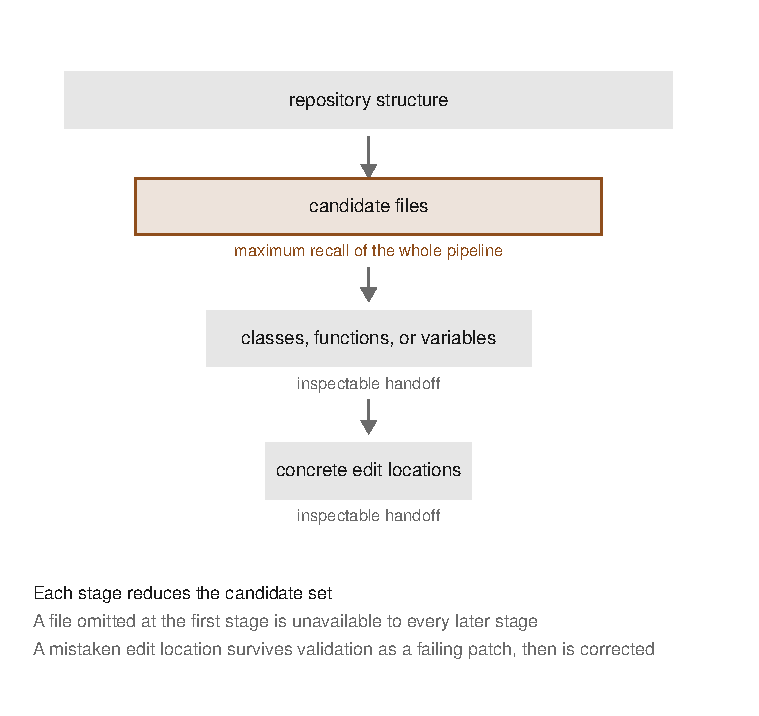
\includegraphics{figures/ch12-localization-funnel.pdf}
\caption{The localization funnel progressively narrows repository evidence, while candidate file selection caps recall because any omitted file remains unavailable to every later inspection and edit stage.}
\end{figure}

Inspectable handoffs make downstream errors visible, but validation can repair a poor edit choice only when the necessary file survived initial selection.

Sepidband et al.~(\href{https://arxiv.org/abs/2604.05481}{2026}) measured this asymmetry across 500 SWE-bench Verified instances and 61 context configurations. Relative to the no-file condition, adding file-level context produced 15 to 17 times as much repair improvement as later localization refinements.

The same experiment found that successful repairs clustered around approximately six to ten relevant files for the model family studied. That range is useful as a diagnostic band, not as a quota for other models, repositories, or task distributions. Both findings come from one benchmark and one sweep of context configurations.

The practical implication is to measure file selection before adding more reasoning downstream. Chapter 11's decomposed scoring makes that diagnosis possible. When file \(\mathrm{Recall}@k\) is low, a stronger patch generator is being evaluated on a candidate set that often excludes the answer. When file recall is already high and repair still fails, additional localization machinery may move cost into a stage that is no longer limiting the system.

\Needspace{5\baselineskip}

The funnel also constrains what context should cross each boundary. A file-selection stage should not silently pass its complete search transcript downstream, because doing so recreates the mixed-granularity problem inside a larger prompt. Its handoff should identify:

\begin{itemize}
\tightlist
\item
  the files retained;
\item
  the evidence for retaining them;
\item
  the candidates rejected; and
\item
  any uncertainty that remains.
\end{itemize}

The next stage can then inspect those files for structural candidates without inheriting every abandoned hypothesis.

Inspectable handoffs also create validation points. Before symbol inspection begins, a file set can be checked against import neighborhoods, ownership boundaries, or another retrieval lane. Before concrete lines are proposed, the symbol set can be checked for definitions, references, and state ownership. These checks need not be performed by an autonomous agent. They need only expose a miss while widening remains possible.

Skipping a stage may appear cheaper because it removes a model call or retrieval pass. Xia et al.~reported the opposite. When their pipeline moved directly from file selection to edit locations, both cost and performance worsened because the remaining stage had to search too much source at once. Removing a stage increased the work inside the stage that remained. Pipeline length is therefore a poor proxy for pipeline cost.

Chang et al.~(\href{https://arxiv.org/abs/2502.15292}{2025}) trained separate models for file, function, and statement localization and found value in treating each level as a distinct representation and discrimination problem. That support is directional and does not determine the implementation. A fixed prompt, cheap classifier, retrieval operation, or stronger general model may be appropriate at a particular stage depending on workload, accuracy, and latency.

The funnel fits issue-resolution work because those tasks often decompose into localization, repair, and validation. It is less convincing for exploratory refactoring, architecture discovery, or changes whose scope becomes visible only after editing begins. Those workloads require an explicit return path that can widen the candidate set after a failed hypothesis. Without one, a rigid pipeline continues refining the wrong corpus.

Later agent systems that surpassed the fixed pipeline also limit any claim that autonomy itself was unnecessary. Stronger models can search, revise, and use tools while preserving hierarchical localization. The evidence supports measuring the fixed narrowing architecture first and then asking which remaining failures autonomy repairs. It does not support freezing the pipeline around one generation of models.

The companion material covers narrower implementation choices: structural retrieval as a lane beside text search, stable structural anchors injected into context, and query-time graph walks when stored expansion would become too large. Those choices follow the architectural decision developed here. Preserve granularity, validate each handoff, and measure file selection as the stage capable of foreclosing every later success.

\hypertarget{build-a-typed-index-only-when-someone-will-maintain-it}{%
\section{Build a typed index only when someone will maintain it}\label{build-a-typed-index-only-when-someone-will-maintain-it}}

Consider an issue reporting that cancelling one export leaves later exports blocked. The change belongs in a generic state-transition helper reached through a queue consumer and shared lifecycle component. None of those artifacts uses the language of exports or cancellation.

Exact search can find the user-facing entry point. Similarity search can find code that resembles the reported symptom. Neither query expresses the dependency path from the entry point to the component that owns the blocked state. A typed index can answer that path question, but the decision to build one begins with maintenance. If no named owner accepts the continuing work, the projected retrieval gain has no durable system behind it.

\Needspace{5\baselineskip}

That work includes:

\begin{itemize}
\tightlist
\item
  parsing each supported language;
\item
  assigning stable identities to entities;
\item
  recording typed relationships;
\item
  handling generated code and partial parses;
\item
  publishing updates without exposing incomplete state;
\item
  versioning the schema and query surface; and
\item
  testing correspondence between index results and repository state.
\end{itemize}

Each new language or artifact type extends the obligation. Index construction is a continuing product surface even when users encounter it only through search results.

The cheaper alternative is often a generated repository map or skeleton placed near the front of the model's context. It can list directories, important files, top-level symbols, and ownership boundaries. Navigation then relies on inexpensive operations such as exact search, opening definitions, finding references, and listing callers.

A repository map cannot answer arbitrary multi-hop questions. It is, however, easy to regenerate and inspect. For a modest repository, low change rate, or occasional task, that trade may be preferable to maintaining a graph service.

A typed index becomes plausible when the workload repeatedly asks structural questions that the map cannot express. The representation parses directories, files, classes, functions, and linked development artifacts into typed nodes. In the export example, invocation and reference edges connect the queue consumer to the lifecycle component and then to the state helper. A broader index may also record containment, imports, inheritance, definitions, ownership, and links to issues or tests.

This representation is a \textbf{typed knowledge graph}. It stores entities under declared kinds and records how each pair of connected entities relates. The types constrain traversal and make a returned path inspectable. They also create schema, parser, identity, and migration obligations that a similarity index does not have.

The export question can then become a bounded traversal:

\begin{verbatim}
start: export handler named by the issue
    -> follow invocation edges into the queue consumer
    -> follow references into the lifecycle component
    -> return functions that write the blocked state
\end{verbatim}

The issue and the final helper need no shared token. The graph supplies a path that can be inspected edge by edge.

A structural path can also be more compact than the alternatives. Instead of serializing the repository or opening every file encountered during exploration, the retriever can return a small subgraph containing the entry point, intermediate calls, state owner, and relationship types. The model receives both the candidates and an explanation of why they were selected.

Published results show why teams consider paying this cost. Chen et al.~(\href{https://arxiv.org/abs/2503.09089}{2025}) reported 92.7 percent file-level localization accuracy for LocAgent, with performance declining at finer granularities. That pattern supports using the graph to protect file localization while measuring symbol and line localization separately. The figure describes localization, not repair, and should not be read as an issue-resolution rate.

LocAgent's fine-tuned 7B and 32B models approached the reported Claude 3.5 localization accuracy at approximately 86 percent lower cost. Its ablations also showed that the gain depended on the complete search and traversal toolset around the graph, not on the stored representation alone.

Yang et al.~(\href{https://arxiv.org/abs/2503.21710v1}{2025}) provide more direct but weaker evidence for multi-hop demand. Among bugs their repository-aware graph successfully localized, 69.7 percent required traversal across several relationships. That figure comes from the first paper revision, and headline results changed later. It also comes from SWE-bench Lite. The result establishes direction within one benchmark, not the prevalence of multi-hop demand in an arbitrary production repository.

The same study capped repair input at the top 20 functions. That cap is part of the architecture. A traversal system can continue finding plausible neighbors after useful evidence has been exhausted. Passing every discovered node to the generator allows additional candidates to interfere with repair. A graph can therefore improve localization while degrading generation when no boundary separates the two stages.

Ma et al.~(\href{https://arxiv.org/abs/2406.01422}{2024}) measured this tension in LingmaAgent across a larger exploration budget. Its issue-resolution rate rose from 16.0 percent with no exploration iterations to 21.3 percent at 600 iterations. Exploration continued to uncover useful code across that range.

The patch-application rate, which measured whether generated diffs applied cleanly, peaked at 200 iterations and then declined through 600. Clean application was necessary but not sufficient for resolution. Fewer patches could apply while more tasks were resolved if the patches that did apply were more often correct. The result suggests that additional exploration continued to improve localization while making the downstream generation problem harder.

Both measurements come from one benchmark configuration. The paper reports the 200-iteration location of the application-rate peak but not the curve's values, so the peak is useful only as a prompt to measure the local stopping point.

A traversal budget must therefore be evaluated against both localization and patch application. It may stop after a fixed number of expansions, when no new relationship type appears, or when the candidate set reaches the repair budget. The literature does not identify one stopping rule that dominates across repositories.

\Needspace{5\baselineskip}

A defensible local rule requires recording:

\begin{itemize}
\tightlist
\item
  each expansion;
\item
  the relationship followed;
\item
  candidates admitted and pruned;
\item
  the downstream candidate limit; and
\item
  the point at which further exploration stopped changing repair outcomes.
\end{itemize}

On SWE-bench Lite, the same study reported an 18.5 percent relative improvement over SWE-agent. That result applies to the benchmark configuration. Its production report used different operating measures: 16.9 percent of in-house issues were resolved automatically and 43.3 percent after human intervention. Automatic resolution, assisted resolution, and benchmark performance describe different systems and should not be combined.

Two additional experiments extend the evidence without removing its limits. Ouyang et al.~(\href{https://arxiv.org/abs/2410.14684}{2024}) added RepoGraph, a line-level definition and reference graph, as a plug-in and reported gains in both pipeline-style and agent-style frameworks. CodexGraph, from Liu et al.~(\href{https://arxiv.org/abs/2408.03910}{2024}), provides directional support for graph queries when similarity retrieval has weak multi-hop recall. Together they support a specialist structural lane that can attach to different orchestration styles.

Fine-grained localization remains difficult. LocAgent's accuracy declined below the file level, and serializing a graph as text can erase distinctions explicit in storage. Edge direction, relationship type, entity scope, and alternative paths can collapse into an ordering the model misreads. Extending the graph below functions may help line-level work, but it also increases node count, serialization cost, and the number of nearly equivalent candidates.

Query construction adds another failure surface. A valid graph can return an irrelevant answer because the model selected the wrong starting entity, followed the wrong relationship, or stopped one hop too early. Bounded operations such as \texttt{find\ definitions}, \texttt{list\ callers}, and \texttt{follow\ imports} are easier to validate than a general graph query generated in one attempt. Simple entity questions should use those cheaper operations, reserving the graph for structural questions that require it.

The representation returned to the model must also be measured. An index may emit paths, source excerpts, signatures, summaries, edge lists, or a combination. Each format changes token cost and the evidence available to the generator. A compact summary may omit the exact call that proves relevance. Raw source may conceal the path that made it relevant. Serialization is therefore part of the retrieval design rather than a presentation detail.

My architecture-analysis toolkit provides one author-system example. Its typed symbol graph measures change propagation by counting files reachable from a changed entity within a bounded depth. The same representation can support impact analysis through relationships that lexical similarity does not encode. This is narrative corroboration and supplies no evidence about agent repair rates.

The index owner must also own correspondence with the repository. Incremental parsers fail, branches diverge, generated artifacts retain obsolete identities, and linked issue data changes independently of code. An index that is not checked against repository state after those events silently answers questions about an earlier repository.

\Needspace{5\baselineskip}

Every returned path should therefore carry enough identity to establish:

\begin{itemize}
\tightlist
\item
  the repository and branch;
\item
  the source revision;
\item
  the index and schema versions;
\item
  the entity identities;
\item
  the freshness status; and
\item
  any parse or ingestion failures affecting the path.
\end{itemize}

Readers unwilling to fund that admission and maintenance path should choose a generated repository map and fixed navigation operations explicitly. Readers willing to fund it should cap candidate sets, budget traversal, validate query construction, test serialization, and measure the graph as one component of the surrounding retrieval system.

The maintenance cost is justified only while a named owner can show which repository state each answer describes.

\hypertarget{admit-only-evidence-tied-to-the-current-state}{%
\section{Admit only evidence tied to the current state}\label{admit-only-evidence-tied-to-the-current-state}}

Weng et al.~(\href{https://arxiv.org/abs/2605.14478}{2026}) changed Python helper signatures in 17 curated examples and compared stale with current retrieved snippets. This small diagnostic study is the only literature support for the practice developed here. It establishes the direction of the failure, but one form of staleness tested on two models supplies neither a general effect size nor a safe refresh cadence.

Under stale-only retrieval, Qwen2.5-Coder-7B-Instruct produced 15 outputs incompatible with the current helper signature, and gpt-4.1-mini produced 13. Both models received the same 17 examples. Under current-only retrieval, neither produced an incompatible output.

These paired results support a narrow architectural rule: retrieved code should enter model context only when the system can tie it to the repository state the worker is allowed to modify.

A stale result is an active hazard rather than an ordinary retrieval miss. It offers a concrete and plausible description of an API that no longer exists. High rank cannot compensate for evidence drawn from the wrong state.

The contrast with no retrieval makes the failure sharper. Without retrieved context, the models tended to fail without calling the obsolete signature. With stale context, they generated executable-looking code against the wrong contract. Retrieval converted uncertainty into a specific but incompatible implementation.

Adding current evidence reduced that harm even when stale snippets remained present. Across the tested model and retrieval conditions, adding valid current snippets to stale ones lowered the rate of current-state-incompatible outputs by 47 to 65 percentage points relative to stale-only retrieval over the same 17 examples. Permuting result order produced no significant difference. In this diagnostic, the presence of current evidence mattered more than whether it appeared first.

The paired comparison corresponds to the binary-outcome design in Chapter 1. Both conditions used the same 17 examples, each outcome was compatible or incompatible, and McNemar's test analyzed the discordant pairs.

The exact two-sided values were \(6.1 \times 10^{-5}\) for Qwen2.5-Coder-7B-Instruct and \(2.4 \times 10^{-4}\) for gpt-4.1-mini. Under the null hypothesis of no difference between retrieval conditions, each value gives the probability of observing discordance at least as extreme as the measured result.

Those values establish a difference within the curated sample. They do not estimate the effect size in another repository.

The study does not show that stale retrieval will fail at similar rates elsewhere, that every form of drift is equally harmful, or that one refresh interval is safe. Helper-signature changes are unusually direct because stale code presents a callable contract. Changes to behavior, configuration, ownership, or surrounding assumptions may fail differently and may be harder to observe.

\Needspace{5\baselineskip}

A freshness gate needs two identities:

\begin{itemize}
\tightlist
\item
  the repository state from which the retrieval artifact was built; and
\item
  the repository state the worker is allowed to edit.
\end{itemize}

A commit identity can represent a clean tree. When relevant files contain uncommitted changes, the commit alone is insufficient because it describes a state different from the worker's current view. The gate then needs content identities for the affected files or another representation of the working state.

Every retrieval response should carry its indexed state identity so the caller can compare it with the working state before exposing any snippet to the model.

The comparison belongs at the retrieval boundary. Checking only when indexing begins leaves a race in which files change during construction or after a long-running query starts. A safe builder reads from a fixed snapshot, constructs the new index privately, and atomically publishes the completed generation together with its state identity. Queries then observe one complete generation rather than a mixture of old and new records.

Suppose an index was built from a clean commit and a worker later edits a helper without committing it. A query returns the old signature together with the index commit. The gate checks the in-scope working file, detects that its content no longer matches the indexed state, and withholds the snippet before generation begins.

Live exact search can supply the current helper while the richer index rebuilds. The builder snapshots the edited state, publishes a completed generation with the new identity, and repeats the original query. The caller admits the new result only after its identity matches the worker's state.

Concurrent work makes the choice of identity important. Two agents may share a base commit while holding different uncommitted edits. A commit-level check can therefore admit evidence stale for both working trees. Hashing every file in a large repository on every query may be too expensive.

\Needspace{5\baselineskip}

A practical design can:

\begin{itemize}
\tightlist
\item
  pin the base commit;
\item
  track content identities for files covered by each response;
\item
  invalidate affected entries from filesystem events; and
\item
  reconcile periodically against the actual working tree.
\end{itemize}

The system should measure both the coverage of that check and the race window it leaves open.

Caches require the same treatment. A query cache keyed only by search text can return an obsolete result after the underlying index refreshes. Repository-state identity must participate in the cache key, or the cache entry must be invalidated when a new index generation publishes. Otherwise the freshness gate protects the index while a faster layer bypasses it.

Retries also need a state transition. If a query fails because its index generation is stale, retrying against the same generation cannot improve the result. The retry must wait for or request a generation built from an accepted state and then repeat the query against that generation.

A timeout can bound the wait, but it should end in an explicit freshness failure rather than silently returning stale evidence.

Refusal has an operational cost. Live exact search may remain current while a structural or semantic index rebuilds. The system can therefore fall back to lower-capability navigation that is tied to the working state. When no current source is available, a visible miss that preserves uncertainty is safer than a fluent answer built from an obsolete API. The generator can request more evidence or fail explicitly rather than act on a false contract.

The literature reviewed for this chapter supplies no universal refresh cadence. Repository change rate, index-build duration, query latency, and the consequence of stale evidence can inform a local policy, but they do not yield an evidence-backed interval.

\Needspace{5\baselineskip}

Event-driven refresh can shorten the stale window after ordinary edits, although missed events and parser failures still require reconciliation. Scheduled rebuilding can provide that reconciliation, but its period should follow measured drift and recovery cost. Useful retrieval metrics include:

\begin{itemize}
\tightlist
\item
  the age of admitted results;
\item
  the frequency of state mismatches;
\item
  the duration of rebuild windows;
\item
  the rate of freshness refusals; and
\item
  the success and cost of fallback navigation.
\end{itemize}

My session-snapshot system illustrates a strict version of this gate. It pins cryptographic hashes for all in-scope files together with the repository commit. Any drift marks the snapshot stale, and the system regenerates it rather than branching from it. Remotely sourced repository knowledge is excluded because the system cannot bind it to the same content check.

My published literature-review index provides the counterexample. One surface advertised a paper count that disagreed with the linked page, and synchronized copies diverged further. The index continued to appear authoritative after it stopped describing its own contents. This contrary case exposes the maintenance cost of the prescription: a freshness policy that no one operates becomes another stale artifact.

Freshness does not determine authorization. Permission policy requires separate identities, rules, and audit records. The evidence here supports refusing obsolete repository states. It does not establish who may retrieve a current one.

\hypertarget{choose-the-next-retrieval-intervention}{%
\section{Choose the next retrieval intervention}\label{choose-the-next-retrieval-intervention}}

Begin with Chapter 11's decomposed measurements and determine which stage is limiting the operated system. Inspect file-level retrieval before changing the agent architecture.

File \(\mathrm{Recall}@k\) asks whether the repair stage receives the necessary files at all. When those files rarely appear, improve file selection and staged localization before adding more open-ended reasoning. A stronger repair model cannot act on evidence the retrieval path excluded.

\Needspace{5\baselineskip}

Next, decide whether repeated structural questions justify a typed index. Before approving the build:

\begin{itemize}
\tightlist
\item
  name the owner;
\item
  define the supported languages and relationship types;
\item
  specify how repository correspondence will be maintained;
\item
  cap the candidates the index can send downstream;
\item
  define its publication and rollback process; and
\item
  record how freshness failures will be detected.
\end{itemize}

When no one owns that lifecycle, choose the cheaper architecture explicitly: a generated repository map near the front of context, together with exact search, definition lookup, reference search, and bounded caller navigation.

Every index, snapshot, and cache should carry a commit or content identity. Compare that identity with the worker's current state at retrieval time. Record mismatches as an operating metric, and refuse the result or fall back to current navigation when the identities differ.

A freshness refusal is visible and recoverable. A stale result can silently become the basis of a plausible patch.

Chapter 13 turns from which evidence the system retrieves to how much of that evidence the model can use.

\textbf{Portable claim.} Evidence without revision identity is stale, not current.

\section*{Sources and evidence}

\textbf{Stage localization before repair}

\begin{itemize}
\tightlist
\item
  Strong evidence: Xia, C. S., et al.~(2024), ``Agentless: Demystifying LLM-based Software Engineering Agents,'' arXiv:2407.01489.
\item
  Directional evidence: Chang, J., et al.~(2025), ``BugCerberus: Bridging Bug Localization and Issue Fixing,'' arXiv:2502.15292. (Per-hierarchy-level specialization.)
\item
  Strong evidence: Sepidband, M., Viet Pham, H., Hemmati, H. (2026), ``On the Role of Fault Localization Context for LLM-Based Program Repair,'' arXiv:2604.05481.
\item
  Corroboration: none on record.
\end{itemize}

\textbf{Index the repository as a knowledge graph}

\begin{itemize}
\tightlist
\item
  Strong evidence: Chen, Z., et al.~(2025), ``LocAgent: Graph-Guided LLM Agents for Code Localization,'' arXiv:2503.09089.
\item
  Directional evidence: Yang, B., et al.~(2025), ``Enhancing Repository-Level Software Repair via Repository-Aware Knowledge Graphs'' (KGCompass), arXiv:2503.21710. (The 69.7 percent multi-hop figure is carried from v1; later versions report different headline values, so the inline link pins v1.)
\item
  Strong evidence: Ma, Y., et al.~(2024), ``Alibaba LingmaAgent: Improving Automated Issue Resolution via Comprehensive Repository Exploration,'' arXiv:2406.01422.
\item
  Directional evidence: Liu, X., et al.~(2024), ``CodexGraph: Bridging Large Language Models and Code Repositories via Code Graph Databases,'' ICLR 2025, arXiv:2408.03910.
\item
  Strong evidence: Ouyang, S., et al.~(2024), ``RepoGraph: Enhancing AI Software Engineering with Repository-level Code Graph,'' arXiv:2410.14684.
\item
  Strong evidence: AOCI AI-oriented code indexing (Liu 2026), arXiv:2605.02421.
\item
  Directional evidence: MAGIS (Tao 2024), arXiv:2403.17927.
\end{itemize}

\textbf{Gate retrieval on freshness}

\begin{itemize}
\tightlist
\item
  Directional evidence: Weng, H., et al.~(2026), ``When Retrieval Hurts Code Completion: A Diagnostic Study of Stale Repository Context,'' arXiv:2605.14478.
\end{itemize}


\chapter{Usable context budgets, consolidated-spec restarts, and file-based tool output}
\label{ch13-usable-context-budgets-spec-restarts-file-output}
Guidance I had placed in a system prompt remained inside the context window twenty turns later but appeared nowhere in the model's stated reasoning. Across 1,705 visible thinking blocks in 199 traces from my trace-diagnostics corpus, that instruction appeared zero times.

Visible reasoning is an incomplete observation of model state, so absence from those blocks does not prove that the instruction had no influence. It does show that material can remain inside the context window without remaining visibly active in the run. Benchmark evidence exposes the same gap through measured performance.

Only about half of the 17 models evaluated by Hsieh et al.~(\href{https://arxiv.org/abs/2404.06654}{2024}) maintained satisfactory performance at 32,000 tokens, even though every model advertised a context window at least that large. Their RULER benchmark combined 13 task types, including retrieval and aggregation.

Rando et al.~(\href{https://arxiv.org/abs/2505.07897}{2025}) found a sharper decline on realistic repository issues as supplied context increased. On LongSWE-Bench, Claude 3.5 Sonnet fell from 29 percent at 32,000 tokens to 3 percent at 256,000 tokens, the model's maximum context in that study. On the separate LongCodeQA task, Qwen2.5-14B-Instruct scored 70.2 percent at 512,000 tokens and 40.0 percent at one million.

The measurement problem is clearer than the prescription. I ranked ten candidate context-assembly practices three times: by how much each would change an engineering decision, how much of the problem it covered, and how teachable it was. The three rankings agreed on only one practice. Five practices appeared in exactly one ranking, and three appeared in none. I take that spread as evidence that the field has not converged. Every recommendation in this chapter is therefore either measured locally or identified as a convention.

The advertised window is a capacity limit. The usable window is a property measured on the work the model must perform.

Once that working limit is known, three assembly decisions follow. A run that has lost its governing specification should restart from a consolidated statement of the settled requirements. Large tool outputs should remain outside the active window in retrievable artifacts. A standing repository context file should be compared with no standing file before its permanent token cost is accepted.

\hypertarget{measure-the-context-that-remains-useful}{%
\section{Measure the context that remains useful}\label{measure-the-context-that-remains-useful}}

I use \textbf{effective context length} to mean the largest assembled context at which a model still meets a specified reliability threshold on a defined workload. The value belongs to a model, configuration, workload, and engineering threshold. A model may accept 128,000 tokens and retrieve one fact at that length while having a much shorter effective context for a code change that depends on relationships among several files.

Measurement begins with task shape. A production coding agent may need to retrieve a declaration from one file, connect it to a caller in another, incorporate a test failure from a third, and preserve a constraint supplied near the beginning of the run. A single hidden fact embedded in filler tests only one part of that work.

\Needspace{5\baselineskip}

The qualification workload should represent the operations the deployed system actually performs, including:

\begin{itemize}
\tightlist
\item
  retrieval across several documents;
\item
  aggregation across several pieces of evidence;
\item
  retention of early instructions;
\item
  reasoning over long code; and
\item
  tool-using trajectories whose context grows over time.
\end{itemize}

The benchmark record shows why these distinctions matter. RULER found that advertised capacity often exceeded the length at which performance remained satisfactory. Leng et al.~(\href{https://arxiv.org/abs/2411.03538}{2024}) evaluated 20 models from 2,000 to 128,000 tokens on retrieval-augmented generation. Accuracy saturated at a model-specific context size, around 64,000 tokens for most frontier models in that study. Beyond that point, model families exhibited different combinations of refusals, repetition, and neglected instructions.

Code work depends more heavily on relationships among units than simple fact retrieval does. Li et al.~(\href{https://arxiv.org/abs/2503.04359}{2025}) introduced LONGCODEU, covering nine models and eight long-code understanding tasks, and found substantial degradation beyond 32,000 tokens despite advertised windows of 128,000 to one million tokens. Understanding relationships among code units was the weakest area.

LongCodeBench evaluated issue answering and bug fixing rather than document retrieval. Its model-task pairs also covered different maximum lengths, so the reported declines belong to those pairs and should not be compared as one curve.

These studies do not identify a universal ceiling. Their results depend on the model generation, prompts, tasks, and scoring rules. The durable finding is the repeated gap between capacity and competence, together with a protocol for measuring it. The knee can move with a new model and may differ between retrieval and code modification even within the same release.

Each study finds degradation within the tested or advertised window. Differences in tasks and metrics prevent direct comparison; the practical response is the local context-size sweep below.

I qualify a model using context-size strata around the range I might deploy. A first pass can include a small condition, two intermediate conditions, and one near the advertised limit. The exact token values depend on the model and workload.

Each stratum should contain the same task families and, when possible, the same underlying tasks with controlled additions to context. This separates the effect of context length from a change in task difficulty.

For repository work, each item begins from a fixed repository state and a known evidence set. The smallest arm receives the minimum material needed to solve the task. Larger arms add realistic neighboring files, test output, prior discussion, generated summaries, or tool schemas in a recorded order.

The model receives the same task, permissions, and tool surface in every arm. I pin the model version, decoding settings, harness version, prompts, and evaluator so that context size remains the deliberate change.

Each stratum is a measured comparison, so Chapter 1's requirements apply. Tasks should be paired across context sizes wherever possible, and every stratum needs repeated independent runs. One run at each length cannot distinguish a context-length effect from ordinary run-to-run variation.

\Needspace{5\baselineskip}

Four outcomes should remain separate:

\begin{itemize}
\tightlist
\item
  \textbf{Retrieval accuracy} records whether the required evidence was found.
\item
  \textbf{Task correctness} records whether the answer or code change was right.
\item
  \textbf{Reliability} records how often the result recurred across repeated runs.
\item
  \textbf{Cost} records tokens, model calls, and tool use.
\end{itemize}

Latency and usability may matter operationally, but neither can substitute for correctness. A longer prompt can reduce retrieval calls while lowering the probability of a correct patch.

I plot outcome distributions by context stratum and reject thresholds based on a single passing run. The \textbf{saturation point} is the region where adding context stops improving the relevant outcome. The operational knee may occur earlier, where the marginal gain no longer justifies added cost or variance.

A decline may be gradual, abrupt, or isolated to one task family. Those shapes support different operating limits.

Suppose retrieval accuracy improves through the intermediate conditions and then flattens, while code-change success begins declining earlier. Retrieval alone would permit a larger budget. The coding workload would not. I set the production limit from the weakest task that must remain reliable, then place retrieval and harness caps below its measured knee.

The margin accounts for token-estimation error, task variation, and fixed context that accumulates during execution. Its size follows consequence. A workflow with cheap retries and deterministic verification may operate close to the knee. A production change with costly failure and weak verification requires more distance.

The final record should state the threshold, uncertainty, and consequence that justified the margin so the decision can be revisited when the system changes.

Several mechanisms can produce decline. Additional context introduces competing versions of facts, similarly named symbols, and relationships the model must reconstruct. Position affects whether early instructions and evidence influence later actions. Repetition can induce repetition, while conflicting material can cause refusal or stale instruction following. The model may also spend more of its output budget restating or reconciling context rather than acting.

\Needspace{5\baselineskip}

Token count alone therefore does not diagnose the failure. I retain traces from every stratum and annotate the first consequential divergence. Useful classes include:

\begin{itemize}
\tightlist
\item
  retrieval failure;
\item
  incorrect symbol relationships;
\item
  forgotten constraints;
\item
  repetition;
\item
  stale or conflicting evidence; and
\item
  harness truncation.
\end{itemize}

The curve identifies where performance weakens. The trace identifies what to change.

This distinction prevents an apparatus failure from being mistaken for a model limit. A harness may silently clip messages at its own cap. An evaluator that sees only the final answer may classify an instruction-following failure as missing knowledge. Larger contexts may also contain more stale repository material, confounding length with freshness.

I therefore preserve the exact assembled prompt, record token allocation by source, and retain every truncation or omission decision with the run.

Context also grows during tool use. A starting prompt well below the limit may cross the measured knee after searches, test logs, edits, and correction attempts accumulate. Qualification should therefore include both static prompts and representative trajectories, or replays of observed context growth.

I measure the initial assembly and the maximum context reached before compaction or restart. A limit applied only to retrieval at time zero does not govern later accumulation.

Every consequential change to the model, workload, or harness requires requalification. A new model may move the knee or change the dominant failure mode. A harness may add standing instructions that consume the safety margin before useful work begins. I preserve the old strata, add cases shaped by the change, and compare the curves.

An unchanged average can conceal a shorter effective context offset by stronger short-context performance. When noise obscures the knee, Chapter 1's power analysis determines whether to add tasks or narrow the claim.

Synthetic probes remain useful because they isolate positional recall, aggregation, and distractor effects. Their thresholds transfer only approximately to repository work. Realistic tasks entangle retrieval, reasoning, tools, and verification, making mechanism attribution harder but deployment relevance greater.

I use synthetic probes to explain a failure and repository-shaped trials to set the operating limit. Neither establishes the other's threshold without measurement.

\Needspace{5\baselineskip}

The final configuration should specify:

\begin{itemize}
\tightlist
\item
  the maximum initial assembly;
\item
  per-source retrieval limits;
\item
  a reserve for tool output and correction;
\item
  the action taken when that reserve is exhausted; and
\item
  the workload and model version that justified each value.
\end{itemize}

A run can remain inside this measured budget and still fail when its specification has become fragmented or superseded.

\hypertarget{restart-from-the-current-specification}{%
\section{Restart from the current specification}\label{restart-from-the-current-specification}}

A model reads the first version of a requirement, resolves an ambiguity, and begins implementing that interpretation. Three turns later, the user corrects the assumption. The correction appears in the transcript, but the plan, file selection, and partial implementation still encode the earlier choice. Each later instruction asks the model to repair work whose structure continues reproducing the misunderstanding.

This can look like stubbornness or weak reasoning. A more useful explanation is commitment under an incrementally revealed specification.

The current task no longer exists in one authoritative place. It is distributed across the initial request, later qualifications, rejected proposals, tool observations, and the model's own accounts of what was decided. Before choosing another action, the system must distinguish accepted decisions from abandoned ones.

Laban et al.~(\href{https://arxiv.org/abs/2505.06120}{2025}) simulated more than 200,000 conversations across 15 models and compared instructions delivered together with instructions spread across several turns. Sharding the instructions produced an average performance decline of 39 percent relative to the single-turn condition. Models showed only slightly lower aptitude but much greater unreliability. They made early assumptions, committed to them, and often failed to recover when later turns supplied missing constraints.

The study used simulated conversational generation tasks. It did not evaluate coding agents operating tools, receiving compiler feedback, or modifying persistent files. Tests and environment errors may correct some assumptions while partial implementations entrench others. I use the 39 percent result as evidence for the commitment mechanism, not as an effect-size estimate for coding work.

The value is also an average across models and tasks rather than a per-conversation quantity. It could represent a few catastrophic failures or smaller degradation across many conversations. Those distributions would justify different interventions.

The trace corpus described at the beginning of this chapter illustrates a related problem without strengthening the causal evidence. Guidance delivered once, twenty turns earlier, remained inside the window but appeared in none of the visible reasoning. Initial delivery is not evidence that a long-running agent still governs its work by the same instruction.

The operational response is consolidation. When requirements emerge through discussion, I rewrite the accepted decisions, constraints, definitions, interfaces, and unresolved questions into one coherent specification. The document identifies itself as authoritative and explicitly supersedes earlier proposals on the same subjects.

It represents the current agreement rather than the chronology through which that agreement emerged.

\Needspace{5\baselineskip}

Consolidation must remain selective because a transcript contains several kinds of state:

\begin{itemize}
\tightlist
\item
  Settled requirements belong in the specification.
\item
  Open questions remain explicitly unresolved.
\item
  Test failures, command output, changed files, and deployment state belong in an execution record.
\item
  Rationale stays with a decision when removing it would invite accidental reversal.
\end{itemize}

The distinction between specification and observation determines what a restart may discard.

Suppose a run has established that an API must remain backward compatible, selected a migration sequence, edited several files, and discovered that a test fixture relies on an undocumented field. The compatibility requirement and migration sequence belong in the consolidated specification. The changed-file list, diff, test command, failure output, and fixture discovery belong in the execution handoff.

Combining both into undifferentiated prose makes it difficult to tell which statements govern future work and which report what happened.

\Needspace{5\baselineskip}

I restart when the run's behavior shows that appended corrections no longer alter its governing interpretation. Indicators include:

\begin{itemize}
\tightlist
\item
  repeatedly proposing an interface that was already rejected;
\item
  continuing to edit files selected under an obsolete plan;
\item
  explaining a current failure through a superseded assumption; or
\item
  spending several turns reconciling conflicting summaries.
\end{itemize}

A growing token count may increase the risk, but it does not determine the boundary. A short run can become incoherent after one consequential misunderstanding. A long run can remain stable when its decisions are consistently restated.

The restart package contains three artifacts.

First, the \textbf{consolidated specification} contains settled requirements and genuinely unresolved questions.

Second, the \textbf{execution handoff} records the repository state, completed changes, current failures, verification already performed, and raw artifacts available for inspection.

Third, the \textbf{starting instruction} identifies the authoritative sources and states the next action.

The package should be built from inspectable state. I use the current diff, test results, issue record, and relevant files as evidence. When a prior claim conflicts with the repository, the repository state governs, and the discrepancy remains visible. A consolidation built from an inaccurate summary produces a cleaner version of the same error.

Restarting has costs. It loses conversational nuance, discarded alternatives, and tacit knowledge about how the work reached its current form. It may repeat exploration or freeze a provisional design too early.

I therefore consolidate only settled decisions. When two designs remain plausible, the specification records both, the evidence supporting each, and the unresolved choice. Consolidation becomes harmful when it silently turns ambiguity into authority.

Environment feedback also resists conversion into static requirements. A failed test may be obsolete, flaky, misconfigured, or decisive. A compiler error is an observation produced against one repository state. The restarted run needs the raw output or a retrievable reference, the command that produced it, and the state against which it ran.

A polished sentence may erase the uncertainty the next investigation needs to resolve.

Versioning prevents authoritative specifications from competing. Every consolidation receives an identity, names the prior version it supersedes, and remains visible to the run. Concurrent workers submit changes through one owner or merge process because requirements that govern all workers require an ordering rule.

A failing run should not decide alone that its interpretation is accurate enough to preserve. The restart boundary belongs to the control plane and should incorporate the trace, repository state, verification results, and user decisions. The model may draft the consolidation, but an inspectable comparison should show what it retained, changed, omitted, or marked unresolved.

High-consequence requirements warrant human review before the new run treats the specification as authoritative.

The choice is between continuing from entangled state and paying to reconstruct clean state. Appending another correction is inexpensive when the run has incorporated earlier corrections and its working interpretation remains coherent. Restarting becomes cheaper when every new turn must fight decisions embedded in the existing trajectory.

The 39 percent result helps explain why repeated correction messages can fail even when a model can solve the same task from a complete specification. When that pattern appears, restart from a consolidated statement of the settled requirements and carry execution evidence separately as raw observations rather than conclusions.

\hypertarget{move-bulk-output-out-of-the-active-context}{%
\section{Move bulk output out of the active context}\label{move-bulk-output-out-of-the-active-context}}

In my agent fleet, a snapshot of the shared skill catalog once traveled between sessions through an environment variable. As sessions inherited, transformed, and re-emitted it, the snapshot drifted. Moving the same context surface into a fingerprinted file made each session's copy atomic and allowed every reload to validate its identity.

The incident illustrates how a named artifact can make ownership, validation, and retrieval explicit. Model-performance effects require a separate comparison.

The evidence for file-backed tool output is limited to two directional practitioner accounts and no strong studies. I treat it as a convention because it is a simple way to control raw-output growth. Long terminal sessions, search results, test logs, tool responses, and pre-compaction history move into session-scoped artifacts. The active context retains a concise description, a stable pointer, and enough metadata for the agent to decide whether loading more is worth the cost.

This changes where state lives. Without externalization, a tool response exists only in the conversation history. Truncation can remove it, while summarization replaces it with an interpretation produced before anyone knows which details will later matter.

\Needspace{5\baselineskip}

With an external artifact, the raw output belongs to the run rather than to the current context window. The active context can retain an index entry containing:

\begin{itemize}
\tightlist
\item
  the command or tool call;
\item
  the time and completion status;
\item
  the byte or token size;
\item
  a content fingerprint;
\item
  the artifact location; and
\item
  whether the content is complete or truncated.
\end{itemize}

Retrieval then becomes incremental. An agent can inspect the final lines of a failed build, search for an error code, or load a bounded range around a match. After a context reset, the replacement run can query the original output instead of relying on a lossy summary. Bulk evidence remains available without occupying the working window on every turn.

The pointer should expose the cost before loading the content. My memory system follows this pattern. An index operation reports the expected token cost, and a separate content operation loads the requested material. Injected lessons can cite their evidence while leaving the raw trace unloaded. The agent may choose a short excerpt when the complete artifact would consume too much of the working window.

Cursor's engineering blog (\href{https://cursor.com/blog/dynamic-context-discovery}{2026}) reports writing long tool output to files that the agent can read back, reducing forced summaries near the context limit. The Hightouch team, in an interview published by Amplify Partners (\href{https://www.amplifypartners.com/blog-posts/how-hightouch-built-their-long-running-agent-harness}{2026}), describes buffering large tool results similarly and reports that the design kept the active window focused on reasoning rather than raw output.

Hightouch also reported that allowing the model to choose when to buffer performed better for its system than a coded decision tree. These accounts provide implementation direction rather than a controlled comparison. Model-selected buffering remains probabilistic, and another model or prompt may make worse choices.

\Needspace{5\baselineskip}

A safe interface therefore places deterministic controls around that choice. The harness owns:

\begin{itemize}
\tightlist
\item
  maximum inline output size;
\item
  artifact-write error handling;
\item
  retention limits;
\item
  access controls;
\item
  permitted read ranges; and
\item
  the behavior when preservation fails.
\end{itemize}

The model may choose among tail, search, range read, and full load within those limits. A failed write returns an explicit failure. The system must not claim that output was preserved when no artifact exists.

Pointers must remain valid across restarts. A path tied only to one temporary process may disappear before a replacement worker can use it. I associate each artifact with a run identity and tool-call identity, preserve ordering, and record completeness. Concurrent calls write distinct artifacts and publish their pointers atomically so one worker cannot overwrite another's evidence.

Security policy follows the data. Terminal output may contain credentials, proprietary source, personal information, or production identifiers. Removing it from the prompt may reduce incidental exposure during later turns, but it also creates a retained artifact that requires permissions, redaction, encryption where appropriate, and a deletion policy.

A pointer must not allow the model to read outside the session's authorized scope. Retention and pointer validity are one decision: deleting an artifact also invalidates every pointer to it in an older transcript.

Files are an implementation choice rather than the essential abstraction. An object store, content-addressed artifact service, or trace database may offer stronger retention and concurrency guarantees. Files are useful early because existing tools can search and range-read them, their failure modes are visible, and they avoid committing to a more elaborate service before the access patterns are understood.

The durable requirement is retrievable raw evidence behind a stable, costed pointer.

Externalization addresses only one source of context growth. Plans, speculative explanations, corrections, and abandoned approaches still accumulate in the active window. A run can write every log to disk and still lose its specification. Compaction and restart from a consolidated specification remain separate controls.

The convention also introduces retrieval failures. An agent may never follow the pointer, search for the wrong term, or load an excerpt that omits the decisive line. An index may point to deleted content. A summary may misdescribe an artifact and discourage inspection.

I therefore retain the raw output, validate pointer resolution, expose search and range operations, and record which portions the agent actually loaded.

\Needspace{5\baselineskip}

The first tests are operational:

\begin{enumerate}
\def\labelenumi{\arabic{enumi}.}
\tightlist
\item
  Can a replacement run recover a required detail after context reset?
\item
  Do concurrent calls preserve separate outputs?
\item
  Does every excerpt resolve to its original artifact?
\item
  Are truncation and failed writes visible?
\item
  Do expired artifacts invalidate their pointers explicitly?
\end{enumerate}

Only after those mechanics work does task-level evaluation ask whether the convention lowers cost or improves completion on workloads with large outputs.

That comparison inherits the resolution problem from Chapter 1. A difference smaller than run-to-run variation can still be measured, but doing so requires enough paired runs. I size the evaluation around the smallest cost or completion change that would alter the engineering decision and interpret the interval around the paired difference rather than one pair of totals.

The current justification is inspectable preservation and ownership. Improvement in task outcomes remains unmeasured.

\hypertarget{make-standing-context-earn-its-permanent-cost}{%
\section{Make standing context earn its permanent cost}\label{make-standing-context-earn-its-permanent-cost}}

Gloaguen et al.~(\href{https://arxiv.org/abs/2602.11988}{2026}) tested whether repository context files already used by coding teams improved task success. Across the evaluated agents and models, they did not. The files increased inference cost by roughly 20 percent, even though the agents followed their instructions.

This is a null result from one study. It should reverse the assumption that a standing context file is beneficial by default, without becoming a universal verdict against such files.

Khatri (\href{https://arxiv.org/abs/2607.27250}{2026}) ran a second controlled ablation across two agents, 17 real tasks from three repositories, and 288 evaluated runs. Equivalence tests bounded any correctness effect to no more than roughly 10 to 15 percentage points and found no measurable improvement. This null result strengthens the case for a no-file baseline while remaining limited by the agents, repositories, tasks, and equivalence bounds studied.

Instruction adherence and task completion measure different effects. A file can cause an agent to run a command, follow a naming rule, or avoid a directory while leaving the final task score unchanged. It can also consume context, provoke additional tool calls, or direct attention toward an overview the model did not need.

Evidence that the file was read and followed establishes treatment delivery; task and cost outcomes determine benefit.

The null result must be interpreted through the power analysis from Chapter 1. Failure to detect improvement may mean that the average effect is small, that positive and negative effects cancel across the task mix, or that the experiment could not resolve the effect it sought.

The measured cost remains part of the result, as does the evidence that the files changed agent behavior. Repositories, instruction categories, models, and safety outcomes may produce a different balance.

The local decision requires a no-file baseline. The same representative tasks and repository states run under the same model, prompts, tools, harness, and evaluator with and without the standing file. The comparison is paired by task, and repeated runs remain necessary when model variation is material.

\Needspace{5\baselineskip}

Before executing the comparison, I record:

\begin{itemize}
\tightlist
\item
  the primary task-success metric;
\item
  cost measures;
\item
  model and harness versions;
\item
  decoding settings;
\item
  the context-file revision;
\item
  the task-set version; and
\item
  the decision threshold.
\end{itemize}

This prevents an unfavorable result from being rescued after the fact by whichever secondary measure happened to move. Diagnostic measures such as instruction adherence, tool calls, latency, and failure class remain useful for explaining the primary result.

Inference cost includes more than the file's input tokens. An instruction may trigger additional searches, builds, reviews, or explanations. A concise repository-specific command may instead prevent failed exploration and lower total cost despite adding permanent context.

I therefore record input and output tokens, model calls, tool execution, and cost per completed task. File length alone is incomplete. A reported 20 percent aggregate difference is also one estimate and deserves the same repeated measurement as a completion score.

\Needspace{5\baselineskip}

The task sample must exercise the claims the file makes. A suite of isolated function edits says little about migration rules, generated code, deployment checks, or concurrent changes. I include:

\begin{itemize}
\tightlist
\item
  ordinary repository work;
\item
  tasks that encounter unusual local constraints; and
\item
  tasks where violating a rule would produce a consequential failure.
\end{itemize}

Expected use determines the mix.

An all-or-nothing comparison may hide which content helps or harms. When the task budget permits, I ablate instruction categories separately. One arm may retain only build and test commands, another only failure-prevention rules, and another the architectural overview.

The categories can interact, so the decomposition is imperfect. It is still more informative than concluding that the entire file either works or does not.

The Gloaguen et al.~result gives narrow failure-prevention rules a plausible role because agents followed the instructions even when aggregate task success did not improve. Permanent inclusion still requires a rule-specific outcome and cost test.

A rule such as ``do not regenerate this checked-in directory manually'' names a concrete failure and can be tested on tasks that encounter that directory. A page describing the repository architecture may duplicate information that search can retrieve only when needed.

I therefore give permanent inclusion a high bar. The default file should focus on unusual constraints and failure-prevention rules that a capable agent is likely to miss and cannot cheaply discover at the moment of need. Common language conventions, framework summaries, and directory tours usually belong behind on-demand retrieval instead.

One of my repositories uses its context file as a failure-mode ledger. Each prohibition names the incident class it prevents. That design connects a rule to a repository-specific need and allows its removal when the hazard disappears. This author-system example illustrates maintenance practice but provides no measured completion benefit.

Actual context files are broader. Chatlatanagulchai et al.~(\href{https://arxiv.org/abs/2511.12884}{2025}) analyzed 2,303 files from 1,925 repositories. Implementation details appeared in 69.9 percent, architecture information in 67.7 percent, and build or execution guidance in 62.3 percent. Security and performance guidance each appeared in 14.5 percent.

Those percentages describe what maintainers wrote, not what improved outcomes. The relative absence of security and performance guidance is a useful review prompt because coding agents can execute commands and modify production-relevant code; it is not a reason to add generic text without a concrete local failure mode.

\Needspace{5\baselineskip}

A file retained after evaluation should be maintained like configuration. Every instruction needs:

\begin{itemize}
\tightlist
\item
  an owner;
\item
  a reason for existing;
\item
  a failure or outcome it is meant to affect;
\item
  a review trigger; and
\item
  a deletion condition.
\end{itemize}

Changes should arrive as small diffs so reviewers can see which behavior is intended to change. Large generated rewrites make stale claims and contradictions harder to detect.

Chatlatanagulchai et al.~also found that context files often evolve through frequent small additions. That observation is compatible with configuration-like maintenance but says nothing about the quality of the changes. A new line may document a real failure, duplicate an existing rule, or preserve an obsolete workaround. Change frequency is not correctness.

Staleness is especially dangerous because the file is authoritative by placement. An obsolete build command can cause the agent to modify generated output or skip a required check. An architectural overview decays as files move. A prohibition tied to a removed failure mode can continue shaping every run after its justification disappears.

I have seen this drift in my own agent-facing documents. A review-checker file contained 35 rules while its header and wrapping skill still claimed 29. A skill-library README contained three incompatible counts. Neither document had a mechanism capable of detecting the discrepancy.

These cases do not measure task impact. They show that documents consumed by agents can become internally inconsistent when their claims are not checked.

Some claims are mechanically verifiable. Counts can be recomputed, paths validated, commands exercised in a clean environment, and generated sections tied to source fingerprints. Another of my knowledge maps stores a source hash so that changes to the material it describes make drift observable.

Semantic claims still require review, but deterministic checks reduce the surface that depends on human memory.

Ownership should be specific enough to trigger review when the build system, repository structure, release process, or protected failure mode changes. Context assembly should also preserve identity and precedence for requirements repeated across system prompts, repository files, task descriptions, and tool documentation. A pre-run check can detect contradictory instructions before the agent must decide which source governs.

The comparison with no file should be interpreted by instruction category and failure consequence as well as by aggregate completion. A file with no measurable mean benefit may still prevent a rare destructive event that the task suite lacks power to observe. That claim needs a specific threat model, a compliance test, and an explicit cost decision.

A general completion benchmark cannot validate or dismiss safety value when its scoring rule omits the relevant failure.

Correctness, reliability, cost, and usability remain separate columns in the decision record. I retain the no-file condition after the first evaluation because a new model, harness change, or substantial file revision may change both adherence and cost. The earlier result belongs to the configuration that produced it.

When the comparison is inconclusive, adherence cannot substitute for the missing outcome. I report the interval the evaluation supports, inspect whether the sample exercised the file's claims, and decide whether a larger test is justified.

A file may remain provisionally for a concrete safety reason, but the exception and its permanent cost should be explicit. An underpowered null does not prove uselessness, just as instruction compliance does not prove benefit.

The best standing file will often become shorter after evaluation. Rules without a concrete purpose, duplicated repository descriptions, stale counts, and material better served through on-demand retrieval can be removed.

What remains is a reviewed configuration surface whose permanent token cost is tied to an observed failure or measured outcome. That is narrower than claiming that repository context files help, and it is a claim the repository can test.

\hypertarget{set-the-context-operating-limits}{%
\section{Set the context operating limits}\label{set-the-context-operating-limits}}

The companion catalog contains narrower techniques for systems that need them. It covers placing load-bearing evidence near a context edge, testing semantic rather than verbatim recall, compacting at task milestones, pricing compression by completed work rather than token reduction, minimizing always-loaded context, and auditing the assembled prompt as an inspectable artifact.

Each technique changes one part of the context path. None removes the need to measure the complete path on the operated workload.

Begin with one production-shaped task family and run it across several context sizes. Include relevant multi-document evidence, realistic distractors, and the relationships the agent must reconstruct. Measure correctness, reliability, and cost separately. Inspect the traces around the decline and place the harness limit below the measured knee for the weakest task that must remain reliable.

Record the model, workload, margin, and changes that require requalification.

\Needspace{5\baselineskip}

Next, identify one long-running task whose governing specification has become fragmented. Stop appending correction messages. Consolidate the accepted decisions, constraints, and unresolved questions into one authoritative specification. Inspect the repository state and verification evidence, then restart from a package containing:

\begin{itemize}
\tightlist
\item
  the consolidated specification;
\item
  an execution handoff containing raw state and observations; and
\item
  a clear next action.
\end{itemize}

The new run should be able to distinguish what it must obey from what it must investigate.

Move large tool outputs into session-scoped artifacts and retain costed pointers in the active context. Verify recovery after reset, separate preservation of concurrent calls, explicit handling of failed writes, and traceability from every excerpt to its raw source. Treat this as an operational convention until a local paired comparison demonstrates a cost or completion effect.

Finally, compare the repository context file with no standing file on the same tasks and repository states. Record task success, reliability, instruction adherence, total inference and tool cost, and the exact file revision. The roughly 20 percent increase reported in one study is a reason to measure, not a transferable estimate.

The paired comparison determines whether the file earns its permanent cost. Category-level ablations determine which instructions remain.

\Needspace{5\baselineskip}

Together, these controls establish:

\begin{itemize}
\tightlist
\item
  how much context the system admits;
\item
  when a run restarts from a clean specification;
\item
  where bulk evidence lives; and
\item
  which instructions deserve permanent residence in every run.
\end{itemize}

Chapter 14 turns to what survives between sessions and in what form.

\section*{Sources and evidence}

\textbf{Budget to measured effective context}

\begin{itemize}
\tightlist
\item
  Strong evidence: Hsieh, C.-P., et al.~(2024), ``RULER: What's the Real Context Size of Your Long-Context Language Models?'' COLM 2024, arXiv:2404.06654.
\item
  Strong evidence: Leng, Q., et al.~(2024), ``Long Context RAG Performance of Large Language Models,'' Databricks Mosaic Research, arXiv:2411.03538.
\item
  Strong evidence: Li, J., et al.~(2025), ``LONGCODEU: Benchmarking Long-Context Language Models on Long Code Understanding,'' arXiv:2503.04359.
\item
  Strong evidence: Rando, S., et al.~(2025), ``LongCodeBench: Evaluating Coding LLMs at 1M Context Windows,'' arXiv:2505.07897.
\item
  Corroboration: none on record.
\end{itemize}

\textbf{Consolidate the specification and restart lost runs}

\begin{itemize}
\tightlist
\item
  Strong evidence: Laban, P., et al.~(2025), ``LLMs Get Lost In Multi-Turn Conversation,'' arXiv:2505.06120.
\item
  Corroboration, narrative only: the author's trace-diagnostics corpus showed that guidance delivered in the system prompt twenty turns earlier was absent from the visible reasoning: 0\% across 1,705 thinking blocks in 199 traces. The literature result, not this case, carries the claim.
\end{itemize}

\textbf{Persist transient context as files}

\begin{itemize}
\tightlist
\item
  Directional evidence: \href{https://cursor.com/blog/dynamic-context-discovery}{``Dynamic Context Discovery in Coding Agents''}, Cursor engineering blog, 2026-01-07.
\item
  Directional evidence: \href{https://www.amplifypartners.com/blog-posts/how-hightouch-built-their-long-running-agent-harness}{``How Hightouch built their long-running agent harness''}, Amplify Partners engineering interview, 2026-01-20.
\item
  Corroboration, narrative only: the author's memory system exposes token cost before loading content, and the author's agent fleet stopped a drifting skill-catalog snapshot by moving it to a fingerprinted, session-atomic file validated on reload.
\end{itemize}

\textbf{Measure context files and maintain them like configuration}

\begin{itemize}
\tightlist
\item
  Null or conflicting result: Gloaguen, T., Mündler, N., Müller, M., Raychev, V., Vechev, M. (2026), ``Evaluating AGENTS.md: Are Repository-Level Context Files Helpful for Coding Agents?'' arXiv:2602.11988.
\item
  Null or conflicting result: Khatri, P. (2026), ``Do Context Files Help Coding Agents? A Two-Agent Ablation Study on Real Repositories,'' arXiv:2607.27250. Across 288 runs, equivalence tests bounded correctness effects to no more than roughly 10 to 15 percentage points in the studied conditions.
\item
  Strong evidence: Chatlatanagulchai, W., et al.~(2025), ``Agent READMEs: An Empirical Study of Context Files for Agentic Coding,'' arXiv:2511.12884.
\item
  Corroboration, narrative only: the author's systems include a context file maintained as a failure-mode ledger and a knowledge map with a machine-checkable source hash; contrary cases include a review-checker whose live rule count disagreed with its header and wrapper, and a skill-library README with three inconsistent counts.
\end{itemize}


\chapter{Cross-session memory, raw traces, and compaction policies}\label{cross-session-memory-raw-traces-and-compaction-policies}

One of my own memory systems rebuilds its entire derived layer whenever the schema version changes. Nothing in that layer is migrated in place. Three append-only tables, holding lessons, memory events, and provenance events, cross the rebuild boundary through mechanical export and import, and everything else is recomputed from the work record it came from. The arrangement is deliberately inconvenient, and it comes with no comparative evidence that it outperforms a system that rewrites its memory as it goes.

The reason for the inconvenience has been measured elsewhere. Zhang (\href{https://arxiv.org/abs/2605.12978}{2026}) studied memories that language models update continuously and found that they degrade. A production account of Slack's context management described the same general shape. The Agentic Context Engineering synthesis (\href{https://arxiv.org/abs/2510.04618}{2025}) names two of the degradation modes, context collapse and brevity bias. Each rewriting pass optimizes a representation that is already the product of an earlier optimization. Deletion and distortion therefore accumulate without any explicit destructive operation, and routine maintenance damages the evidence.

I treat the complete chronological record of a session's inputs, actions, outputs, and state changes as the ground truth for cross-session memory. I call that record the raw, or episodic, trace. Everything derived from it must remain rebuildable. Observed query and task failures, rather than anticipated ones, determine when the storage and compression layers deserve more complexity.

The evidence base for this chapter is thin. Six items support its three design entries. Only two of the six are strong, and five are explorer-class syntheses rather than controlled experiments. The storage recommendation has no strong item at all and remains contested among practitioners. I therefore use this evidence to define architectures and measurement decisions. It supplies no defensible retention period, retrieval threshold, or compression ratio.

\section{Preserve the evidence before deriving the memory}\label{preserve-the-evidence-before-deriving-the-memory}

Continuous rewriting can leave the latest stored record without evidence that earlier versions contained. Support for this failure mechanism comes from one explorer-class study the evidence audit retained as strong, one directional synthesis, and the Slack production account named alongside them. The directional synthesis is Agentic Context Engineering (2025). The evidence audit records no quantitative result behind it, and it therefore supports the direction of the practice only. No controlled comparison of storage architectures is on record.

I therefore separate the immutable source record from every summary or fact derived from it. Material removed by an earlier rewrite cannot be recovered from the latest rewrite. A further pass may produce a better summary of the remaining text, but it has no observation from which to reconstruct what disappeared. The system has crossed a recovery boundary without marking the crossing. Treating each rewrite as a new authoritative state hides that loss behind a successful update.

An immutable raw layer changes the failure mode. The store appends the original session events and does not ask a model to modify them. A separate process reads those events and produces a summary, a profile, or a collection of extracted facts. I call that output the distillate, meaning a derived representation built from the source record for later use. When the distillate omits material from the source record, the omission is a retrieval or consolidation defect that can be repaired from preserved evidence.

The architecture has two ownership rules. The recorder owns fidelity to what happened, including ordering, identity, and state references. The distiller owns one interpretation of that record for a stated retrieval purpose. A summary may say what the system believed about a user, while the trace records which statement produced that belief, when it arrived, and what later event contradicted it. Collapsing the two roles into one mutable record converts an inference into history.

Rebuildability follows from that separation. Every derived item carries provenance back to the trace events that produced it and to the version of the extraction or summarization rule that interpreted them. When the schema changes, the system constructs a new derived store from the raw record. It does not ask a model to translate each old conclusion into a new conclusion in place. Parallel rebuilds also let an operator compare the old and new distillates before switching readers to the new version.

\begin{verbatim}
recorder
    -> inputs + actions + outputs + state changes
        -> complete chronological raw, or episodic, trace
           [ground truth: ordering + identity + state references]
                |
                v
distiller -> stated retrieval purpose -> derived store
                |
                +-> provenance -> trace events
                +-> version of extraction or summarization rule

schema changes
    -> raw record -> new derived store

earlier rewrite removes material
    -> latest rewrite cannot recover it
\end{verbatim}

The artifact here is the replayable trace from Chapter 9, used for a second purpose. In recovery, the trace reconstructs execution after a crash. In memory, it reconstructs a representation after that representation proves incomplete or wrong. The requirements overlap, but memory adds access patterns, retention decisions, and user-facing correction obligations that execution replay alone does not settle.

Consider a coding agent that learns three things during a repository investigation. An interface was renamed. A compatibility wrapper remains for one release. One service still calls the wrapper during rollback. A concise summary may retain the rename and the wrapper while dropping the rollback dependency as a low-frequency detail.

Weeks later, an incident task asks whether the wrapper can be removed, and a memory query against the summary returns a confident but incomplete answer. With the raw trace preserved, the system can respond in several defensible ways. It can retrieve the original observation directly. It can rebuild the facts under a schema that represents rollback dependencies. It can show the user that the current summary has no coverage for the question. Without the trace, the only available repair is another model-generated guess.

Continuous rewriting also confuses time. Suppose an early session records that a service owner is Priya. A later session records that ownership moved to Luis. A third task then asks who approved a decision made between those two dates. A profile optimized for the current owner may erase Priya entirely, while preserving both events lets the derived layer represent succession, validity intervals, or uncertainty across time.

This temporal case points to a design the companion catalog develops separately. A memory can supersede a claim for current use while retaining the earlier version for questions about the past. Work on temporal knowledge-graph memory, from Kim et al.~(\href{https://arxiv.org/abs/2408.05861}{2024}), is part of the support. The recommendation of two time axes, one for when a fact was true and one for when the system learned it, is practitioner-weighted rather than a measured result of that work, and it remains directional. The raw event order supplies the observations. The derived schema still has to decide how a claim becomes current, obsolete, or disputed.

Immutability does not mean public access or indefinite retention. Raw traces can contain credentials, personal attributes, proprietary code, and conclusions that later prove false. Their value as recovery material increases the damage from an access-control failure. I classify the raw layer as sensitive source material, restrict writers to append operations, encrypt it under a stated retention policy, and log every reader that crosses the boundary.

Deletion has to follow provenance in the other direction. If a user or a policy requires removal of a raw event, every summary, profile, embedding, cache entry, and graph edge derived from it becomes suspect. A deletion process that removes only the transcript leaves the more convenient copies intact. The system needs a mechanical way to find the affected derivatives, invalidate them, and rebuild what remains from authorized source material.

Forgetting is therefore part of the architecture, and it is the least-measured part of the memory stack in the evidence available here. A system may demonstrate that it retrieved retained facts without testing whether deleted or superseded facts still reach generation through a summary, a cache, or a model-produced profile. Deletion propagation and stale-claim retrieval should therefore be measured separately from task success. A task can succeed while a deleted fact is still shaping the answer.

Retention has a boundary the recovery argument cannot override. Some systems cannot lawfully or safely keep complete traces. Others should not keep them, because the likely harm exceeds their diagnostic value. In these settings, the raw layer may need field-level redaction, a shortened retention window, content-addressed references to separately governed artifacts, or deliberate noncollection. The design requirement is to make each loss explicit and testable. An already compressed record cannot serve as the raw recovery boundary.

\emph{Companion-site aside, thin support:} Persisting the repository regions an agent has already explored may prevent repeated discovery work across sessions. The idea rests on one directional source, from Pan et al.~(\href{https://arxiv.org/abs/2507.19942}{2025}). Whether it reduces redundant retrieval without also preserving stale interpretations should therefore be tested.

\emph{Companion-site aside, thin support:} Durable project state persisted across crashes and context loss in the long-horizon engineering system Chen (\href{https://arxiv.org/abs/2604.13018}{2026}) evaluated. That result is a directional reason to hand off artifact references between agents. No controlled comparison against transcript-summary handoff is on record, and the fidelity advantage over a summary therefore remains an inference. The receiving agent also needs a way to verify artifact identity, permissions, and version.

\section{Make the storage system earn its complexity}\label{make-the-storage-system-earn-its-complexity}

At a new agent project's architecture review, the design already contained a vector database and a knowledge graph. The query log was empty. Nobody had asked the system a question yet, and the retrieval architecture had already been settled.

The support for arguing against that default is directional, practitioner-weighted, and contested. It comes from three explorer syntheses and no strong item. Menschikov (\href{https://arxiv.org/abs/2506.17001}{2025}) compared knowledge-graph memory against lighter substrates in a personal-AI setting. Wolff and Bennati (\href{https://arxiv.org/abs/2601.07978}{2026}) compared cost against accuracy, and the evidence audit classifies that comparison as directional with no quantitative result behind it. Yang (\href{https://arxiv.org/abs/2602.05665}{2026}) surveyed graph-based agent memory, and that survey is the counterweight to the position taken here rather than support for it.

A practitioner argument that knowledge graphs are the wrong abstraction for agent memory runs alongside those papers, with no study behind it. Together these establish a presumption in favor of simpler infrastructure. They do not establish that relational storage wins across workloads.

I begin the decision with the corpus the agent records: session transcripts, tool observations, decisions, outcomes, and the provenance connecting derived facts back to those events. A relational database can store those records with stable identifiers, explicit time fields, access controls, and transactional deletion. Full-text search supplies an inspectable first retrieval path. The operator can see the query, the matched terms, the filters, and the returned rows without first interpreting a learned similarity score or a model-extracted edge.

This starting point is deliberately modest. It handles exact identifiers, quoted phrases, error text, names, paths, and combinations of structured filters with lexical search. It also exposes its own failures. If a user asks for ``the outage caused by stale ownership data'' while the trace says ``the on-call mapping lagged the transfer,'' lexical retrieval may miss the connection. This miss is evidence for a semantic retrieval lane, provided such mismatches recur in representative work.

Vector retrieval adds that lane by comparing learned representations of the query and the stored text. The extra machinery may be justified when users regularly describe the same event in different language, when terminology changes across teams, or when the useful passage shares a concept but few tokens with the query. It also introduces an embedding model whose version and chunking choices change the representation. The additional index needs its own update and deletion path. I assess those costs against observed lexical misses rather than against anticipated ones.

A knowledge graph makes a different promise. It represents entities and relations. The system can therefore traverse a question such as which services depend on a library owned by a team whose runbook changed after an incident. When relationships are the object of retrieval and multi-hop questions recur, the schema and maintenance cost of that representation can be justified. Similarity search is not a reliable substitute for explicit traversal when the answer depends on a chain of named relations.

The graph obtains those relations through an extraction pipeline. A model reads an event or a summary, decides which entities exist, resolves their identities, and emits edges. Each of those decisions can invent content, merge distinct entities, split one entity into several, or assign a relation the trace did not state. A graph can then return a mechanically correct traversal over semantically wrong edges, which makes the answer look better supported than its evidence warrants.

High-degree entities create a separate scaling problem. Common concepts such as production, a central platform team, or a widely used library can become hubs connected to much of the store. Queries through those hubs expand rapidly and return weakly related paths. The operator has to bound queries with relation constraints and temporal filters, and the pipeline has to prune weak edges and repair entity identities. Graph construction then becomes an ongoing information-quality program rather than a one-time schema decision.

The two additions solve different failures. A vector index addresses lexical mismatch. A graph addresses repeated relational traversal. Combining them may serve a workload that needs both, but the combination also compounds the provenance, synchronization, access-control, and deletion obligations. The design record should name which representative queries each component answers and which observed failures made the simpler path inadequate.

The decision has the same shape as Chapter 12's repository-index choice, but the corpora differ. Chapter 12 concerned how an agent indexes a repository that already exists. Here the corpus is the agent's own experience, and the extraction step may create entities or relations that were not present in the source. This difference raises the cost of an opaque derivation error.

Local-deployment claims need the same scrutiny. A memory framework may keep its database on a workstation while sending extraction or embedding requests to a remote model. Another may require a cloud key for the advertised default path even though its storage package is open source. I inspect the effective dependency graph, including model calls, embedding services, telemetry, background synchronization, and credential flow, before classifying a system as local.

Governance can change the preferred substrate before retrieval quality does. A relational transcript store may fit existing backup, audit, residency, row-level access, and deletion controls. A managed vector service might satisfy the same requirements with less operational effort in another organization. A graph may expose sensitive relations that no single source event revealed. Storage cost alone cannot decide among systems that create different privacy and accountability surfaces.

The comparison also has to separate correctness from performance. A full-text query that returns no relevant record has a retrieval-correctness problem even when it completes in milliseconds. A graph query that finds the right path but takes too long under hub expansion has a performance problem. A vector result that is useful but cannot be traced to an authorized source has a governance problem. Collapsing all three into `memory quality' hides which component has to change.

I use a small query set before adding infrastructure. It includes ordinary lookups, paraphrased requests, time-bounded questions, deletion checks, and the relational questions that prompted the discussion. For each query, I record whether the relevant evidence was retrieved, which irrelevant records displaced it, how the answer traces back to source events, what the operation cost, and whether the access policy held.

I draw this set from real tasks and failures, and I write it down before any candidate store is compared. Examples chosen after seeing which store handled them would favor that store, for the same reason Chapter 2 requires a task-exclusion rule to be declared before the outcomes are inspected.

The decision stays reversible while the raw layer remains independent. A vector index can be rebuilt from authorized transcript segments. A graph can be regenerated under a revised extraction schema and compared with its predecessor. If either system becomes necessary, it joins the derived layer and leaves the source intact. The recovery boundary remains intact while the retrieval architecture becomes more specialized.

A simple store can also be a false economy. Repeated lexical misses can force users to restate questions, cause the agent to proceed without prior evidence, and consume review time. Repeated manual joins across records can conceal relations the workload depends on. The presumption for simplicity expires when measured query failures and operating constraints show that the initial system cannot answer the work.

The opposite failure is easier to miss, because the system looks sophisticated while it fails. A graph built for future questions can make schema repair, entity reconciliation, and edge pruning the dominant memory task before any production query uses a traversal. A vector lane can accumulate embeddings whose source text has been deleted or superseded. Those maintenance costs belong in the same evaluation as the retrieval gains.

Scheduled consolidation into typed, pruned records can reduce query-time work once the types correspond to recurring retrieval needs. Scheduling changes when interpretation happens. It does not change the evidence boundary, because every consolidated item still needs source provenance and a rebuild path. Consolidating on a timer before the types have stabilized moves speculative extraction into a batch job.

Product and decision context may also need to be stored separately from code search. Dillon (\href{https://arxiv.org/abs/2605.08112}{2026}) measured coding-agent decision compliance when recorded product, design, and engineering decisions were available to the agent, and that support is directional. Extending it to runbooks, ownership changes, rejected designs, and incident lessons is an inference, though each of those answers questions that repository structure cannot. Such material should be stored under explicit source and time semantics, and code search should stay scoped to the repository.

\emph{Companion-site aside, thin support:} Memory portability favors exportable events, explicit schemas, and provenance another system can audit. The support, from Munirathinam (\href{https://arxiv.org/abs/2606.01138}{2026}), is anecdotal. A portability claim should therefore be tested with an actual export and import. A feature claim in a product description is not a test.

\section{Tune compaction against failures}\label{tune-compaction-against-failures}

A reviewer opens a failed trace annotated under Chapter 10's protocol and finds that the first upstream error followed a condensed-history update. Compaction is the replacement of working history with a condensed representation so a run stays inside its context budget. A fixed summarization prompt looks like routine maintenance, and its error profile goes unmeasured. One policy may preserve goals while dropping constraints. Another may retain decisions but blur which tool observation supported them. A third may keep every apparent dependency and fill the effective context length with obsolete branches.

The evidence for treating compaction as a tunable artifact rests on one strong literature study, from Kang et al.~(\href{https://arxiv.org/abs/2510.00615}{2025}), covering app, office, and question-answering agents. It includes no coding-agent benchmark. Transfer to repository work therefore remains an inference. That study supports treating each policy as a candidate component whose omissions, distortions, and distractions can be observed on tasks rather than assumed.

Chapter 10's protocol asks the reader to grow the corpus toward one hundred diverse traces and to cluster it into five to ten failure classes, assigning the first upstream error in each run. Those counts are unmeasured starting recommendations. For compaction, I add a context label only when the preserved trace supports it. The label states whether necessary evidence was missing, retained with changed meaning, or present but obscured by irrelevant history. It also records the compaction version and points to the source events that should or should not have survived.

This label is an attribution judgment rather than a measurement. Chapter 10 requires a named human to sign any attribution that changes remediation or the interpretation of an evaluation, and a change to the compaction policy is exactly such a decision.

The label also prevents a common attribution error. A task can fail after compaction even when memory played no causal role. The repository may have changed, a tool may have timed out, or the agent may have ignored evidence that remained plainly available. I revise the policy only when the trace supports a counterfactual claim. The claim is that a different representation of the same prior history could have changed the relevant decision.

The first policies are therefore hypotheses. Before any failure corpus exists, I can specify structural rules such as retaining current goals, unresolved constraints, artifact identities, decision provenance, and contradictory observations. I cannot know their relative value for a particular workload. The early system should preserve the raw material, record which rule produced each condensed history, and avoid presenting an untested prompt as optimized.

Once failures accumulate, I change one policy element at a time. A rule might preserve the exact observation behind an unresolved dependency, distinguish superseded facts from deleted facts, or discard completed exploratory branches after their artifacts have been recorded. I then re-run paired repeats on the same tasks using the discipline from Chapter 1. The comparison measures task success and the context used, and token count remains a secondary resource measure.

A comparison of two compaction policies is subject to the run-to-run variance Chapter 1 describes. One run of each policy is one draw. A difference that stays smaller than the measured spread should therefore not justify replacing the incumbent policy.

The compatibility-wrapper case provides a concrete policy test. The raw trace records that one service still calls the wrapper during rollback, while the compacted history drops that observation. The agent recommends removal, and the reviewer marks the recommendation as the first upstream error, caused by missing context.

I revise one rule so that unresolved rollback dependencies retain their source observation, then rebuild the condensed history from the same raw trace. Paired runs on the same removal task show whether the agent now preserves the wrapper and uses the retained evidence. I accept the change only when task success improves without a new distraction failure on neighboring cases. Otherwise the policy stays a hypothesis.

Kang et al.~reported peak-token reductions of 26 to 54 percent alongside improved task success across three app, office, and question-answering benchmarks. They also reported gains of up to 46 percent for small-model agents when distracting context was removed. Under those experimental designs, less context coincided with better reasoning. Those results do not establish an expected reduction or an expected success gain for coding agents.

\begin{figure}
\centering
\pandocbounded{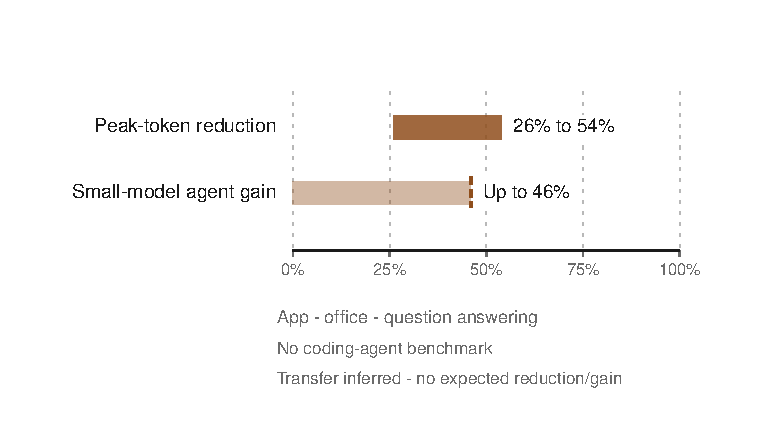
\includegraphics[keepaspectratio,alt={Across app, office, and question-answering agents, removing distractions cuts peak tokens by 26\% to 54\% and raises small-model success by up to 46\%; no coding-agent benchmark supports extrapolating either effect to coding agents.}]{figures/ch14-compaction-tokens.pdf}}
\caption{Across app, office, and question-answering agents, removing distractions cuts peak tokens by 26\% to 54\% and raises small-model success by up to 46\%; no coding-agent benchmark supports extrapolating either effect to coding agents.}
\end{figure}

The study covers app, office, and question-answering benchmarks, with no coding-agent benchmark; repository transfer remains an inference without an expected coding-agent reduction or gain.

The plausible mechanism is the work required to discriminate among records. A model presented with every prior attempt has to decide which constraints remain active, which observations are stale, and which abandoned branches should influence the next action. Irrelevant history competes with useful evidence for attention, and repetition can make an obsolete plan look current. Removing that material can improve correctness while also reducing inference cost.

Compression creates the inverse failure. A concise history may omit a rare constraint because it contributed few tokens or appeared only once. Frequency is a poor proxy when one low-salience fact controls whether a destructive action is permitted. The failure corpus reveals which details became decisive in actual investigations, and the policy can then preserve evidence by function rather than by apparent prominence.

Task success alone is still too coarse for diagnosis. I inspect whether the compacted context retained the decisive observation, preserved its qualification, and excluded material that had become irrelevant. A successful run can hide a damaged memory when the model guessed correctly or recovered through a tool call. A failed run can show a sound compacted context that the model then misused. Keeping those cases separate prevents the compactor from absorbing every downstream error.

Policy versions have to remain replayable. The same raw trace should produce the same condensed representation under a named policy and model configuration, or the rebuild has to record its nondeterminism explicitly. When retries occur, the system records whether they reuse the existing compacted state or rebuild from the raw trace. Otherwise a successful retry can conceal that the first and second attempts received different histories.

When a tuned policy stabilizes across new failures and held-aside traces from the same workload, its examples can train or distill a smaller model. This step changes latency and cost. It also creates another component to evaluate for semantic drift. The smaller model's outputs and downstream task behavior should therefore be compared against the accepted policy, and a route back to the larger compactor should stay open for cases it cannot handle.

The loop cannot start on the first day, because no local failure evidence exists yet. Borrowed rules can supply a safe initial hypothesis, and preserving raw traces can limit the cost of a wrong initial policy by making its derived representation rebuildable. Optimization begins only after the traces show which omissions and distractions cause errors. The dependency on Chapter 10's corpus is the reason compaction tuning comes after the rest of the retrieval and context architecture rather than before it.

\section{A staged protocol for recoverable memory}\label{a-staged-protocol-for-recoverable-memory}

Storage and retention decisions take effect in the first session. Revision of the compaction policy waits for Chapter 10's failure corpus. The sequence below separates the immediate controls from the evidence-dependent ones.

From the first run, I keep every permitted raw trace in inexpensive immutable storage, and I mark every summary, profile, extracted fact, vector, and edge as derived. I record provenance and policy versions before the derived layer becomes operationally important. I test retention limits and deletion propagation as part of the design, because a recovery boundary that violates its governance boundary cannot stay in service.

I start retrieval with a relational transcript store and full-text search. This start is a presumption drawn from contested, directional evidence, not a measured result. Observed local query failures justify moving beyond it. Before adding another lane, I write down the representative queries and the observed failures that would justify it: recurring lexical mismatch for vectors, recurring relational traversal for a graph. Operating cost, dependency exposure, deletion behavior, and access control belong in that decision.

I run the first compaction rules as hypotheses and keep their outputs reproducible from the raw trace. Once the Chapter 10 corpus contains context-caused failures, I revise the policy against those cases and re-measure task success on paired tasks. Token reduction is a capacity-planning number. It cannot substitute for evidence that the agent made better decisions.

Review capacity is a finite input, and it does not grow as the fleet grows. Part V takes up the people who answer for this work, and the interfaces and escalation rules built around their limited attention.

\section{Sources and evidence}\label{sources-and-evidence}

The evidence class and strength on each entry below come from its catalog record. Author-system cases in this chapter are narrative illustration and are not part of the evidence base.

\subsection{Preserve raw traces and distill separately}\label{preserve-raw-traces-and-distill-separately}

\begin{itemize}
\tightlist
\item
  explorer/strong: ``Useful Memories Become Faulty When Continuously Updated by LLMs'' (Zhang 2026), arXiv:2605.12978, with Slack production context management (InfoQ 2026-04) named in the same synthesis.
\item
  explorer/directional: Agentic Context Engineering, arXiv:2510.04618. Direction only.
\item
  Corroboration (narrative only): the author's memory system rebuilds its derived layer on schema changes and mechanically carries three append-only event tables across rebuilds.
\end{itemize}

\subsection{Use a light store by default}\label{use-a-light-store-by-default}

\begin{itemize}
\tightlist
\item
  explorer/directional: PersonalAI KG comparison (Menschikov), arXiv:2506.17001, with a contested practitioner thread named in the same synthesis. Direction only.
\item
  explorer/directional: Cost-and-Accuracy study (Wolff \& Bennati 2026), arXiv:2601.07978. Direction only.
\item
  explorer/directional (boundary citation): Graph-based Agent Memory survey (Yang 2026), arXiv:2602.05665. Cited as the counterweight, not support.
\item
  Corroboration: none on record.
\end{itemize}

\subsection{Optimize compaction from failures}\label{optimize-compaction-from-failures}

\begin{itemize}
\tightlist
\item
  lit/strong: Kang, M., et al.~(2025), ``ACON: Optimizing Context Compression for Long-horizon LLM Agents,'' arXiv:2510.00615 (Microsoft).
\item
  Corroboration: none on record.
\end{itemize}

\subsection{Companion-catalog records named inline}\label{companion-catalog-records-named-inline}

These are not part of this chapter's three taught entries. Each is named in the prose so a reader can follow the aside to its source, at the strength the record carries.

\begin{itemize}
\tightlist
\item
  explorer/directional: Temporal KG memory (Kim et al.), arXiv:2408.05861, carried by the companion record on modeling time explicitly. Supports the two-time-axes aside only.
\item
  lit/directional: Prometheus (Pan, H., et al.~2025), arXiv:2507.19942, carried by the companion record on persisting explored context. No figure quoted here.
\item
  explorer/directional: AiScientist long-horizon engineering (Chen 2026), arXiv:2604.13018, carried by the companion record on durable artifact handoff.
\item
  explorer/anecdotal: memorywire (Munirathinam 2026), arXiv:2606.01138, carried by the companion record on memory portability.
\item
  explorer/directional: Product context and coding-agent decision compliance (Dillon 2026), arXiv:2605.08112, carried by the companion record on the tribal-knowledge substrate. Its compliance figure is not used in the prose.
\end{itemize}

Author-system cases in this chapter are narrative illustration, not evidence.


\part{Human review and accountability engineering}

\chapter{Efficient verification interfaces and risk-based human escalation}\label{efficient-verification-interfaces-and-risk-based-human-escalation}

On my own site, every agent output arrives as a schema-validated Git diff. The agent cannot write to the production database or publish a page. That architecture places the proposed state transition in an artifact I can read, execute, reject, or revise before it acquires production authority. It provides no evidence that the output is correct. A diff that is easy to approve looks a great deal like a diff that has been checked.

A reviewer skimming that diff is making a cost-benefit decision. Reading every changed branch, reconstructing the intended behavior, running the relevant tests, and checking the result against the task costs far more than a single approval click. When the expected consequence of a missed defect feels remote, that cost difference makes shallow review the rational response, even for a reviewer who intends to be careful.

Vasconcelos et al.~(\href{https://arxiv.org/abs/2212.06823}{2023}) tested this account across five experiments. Their subject was overreliance, the reliance failure in which a person accepts an incorrect AI output. It changed when the economics of checking changed. Participants engaged more when verification required less effort or when the cost of an error became more salient. Explanations reduced overreliance when they altered that calculation. They did not work as a general antidote to misplaced trust.

This result changes the engineering question. Telling reviewers to be more careful treats attention as a personality trait. A review system has to account instead for the price of obtaining evidence, the point at which a person can accept an output, and the finite supply of human judgment. Those are properties of the workflow, and they can be inspected and changed.

Review capacity does not grow because a fleet can produce more patches. Practitioner reports already describe systems generating substantial code volume behind retained human gates. InfoQ reported (\href{https://www.infoq.com/news/2026/03/stripe-autonomous-coding-agents/}{2026}) that Stripe's Minions system produces more than 1,300 production pull requests per week. The figure says nothing about review depth, defect escape, or whether the gate changed any verdict, which is the part I would want to know. It does illustrate the queueing problem. Generation can scale faster than the people authorized to accept its consequences.

I treat this mismatch as three connected design problems. The review surface has to make a correctness claim cheap to challenge. Friction has to interrupt the fast accept loop without taxing every interaction equally. Automated monitors have to concentrate scarce human attention on the cases that warrant judgment, while the verdict stays with a named person. Each intervention changes the cost or the allocation of review. None of them creates correctness.

Nearly all of the empirical oversight results I have used here predate long-horizon agents. In my reading of that work, researchers have rarely tested whether findings about people reviewing suggestions carry over to autonomous actions, although they commonly assume that they do. A code completion that waits for a programmer to accept one function and an agent that edits files, runs commands, revises its plan, and opens a proposed patch create different observability and control problems. The older evidence is useful for identifying mechanisms. It does not settle how those mechanisms behave after autonomy, duration, and action space increase.

The practical standard is therefore narrower than `keep a human in the loop.' A loop can contain a human who sees too little, arrives too late, has no affordable way to check the work, or lacks the authority to stop it. The questions worth asking are concrete. What evidence reaches the reviewer? At which decision is independent judgment required? Which cases consume scarce review time? Who owns the final verdict, and what happens after that person decides?

\section{The price of a check}\label{the-price-of-a-check}

An explanation describes why an output might be right. A verification interface gives the reviewer a practical way to discover that it is wrong. Tests, executable examples, types, continuous-integration gates, sandboxed runs, and evidence placed next to the claim all serve the second purpose. Their value comes from the failures they can expose.

Suppose an agent changes a retry loop. A prose rationale might say that the new backoff prevents overload while preserving responsiveness. A useful review surface shows the changed state machine, the maximum attempt count, the errors classified as retryable, and a test that advances a fake clock through failure and recovery. The reviewer can then challenge specific claims: whether retries stop, whether a non-retryable error escapes immediately, whether cancellation is honored, and whether two workers can duplicate the side effect. The explanation may help locate those claims. The executable evidence does the checking.

The same principle governs evidence presentation. Admission to the review surface and inspection within an artifact are different decisions. A system may correctly decide that logs, traces, generated files, and dependency changes belong in the review packet and still bury the relevant event among thousands of lines. Curating what reviewers see helps only when the omitted material remains reachable and the curation rule itself can be inspected. Otherwise the interface reduces apparent complexity by hiding the evidence needed to falsify the output.

Fok and Weld (\href{https://arxiv.org/abs/2305.07722}{2024}) synthesized the research on explainable AI and reached a compatible but directional conclusion. Explanations rarely produced complementary performance, in which the human and the AI together outperform either one alone, unless the explanation helped the person verify the answer. That literature spans tasks with different error costs, expertise requirements, and verification opportunities, so it does not justify a universal claim that one explanation format will improve code review. It does support a sharper design test. After reading the explanation, what can the reviewer now check that was previously too expensive or unavailable?

Software is unusually favorable under that test. Many software claims admit partial mechanical oracles. A compiler can reject a type error. A property test can generate cases a reviewer would not enumerate. A deterministic replay can expose an ordering fault. A sandbox can show which files and network endpoints an action touched. None of these proves total correctness, but each can move a claim from something the reviewer has to read and trust toward something the reviewer can run and challenge.

The favorable case has strict boundaries. A passing test suite establishes only that the tested behavior passed under the tested conditions. Generated tests can repeat the implementation's mistaken assumption. Type systems encode some properties and omit others. Sandboxes constrain consequences without establishing intent. A green continuous-integration result can itself become a trust signal that accelerates acceptance, even when the changed risk lies outside the suite.

A large diff with weak tests can therefore leave verification more expensive than acceptance. The reviewer has to reconstruct behavior across files, infer unstated requirements, and judge interactions that no executable check covers. Adding a longer reasoning trace increases reading cost without creating an oracle. Under those conditions, the cost-benefit account predicts shallow engagement.

Optimizing first for the completeness of an agent's explanation is therefore the wrong starting move. The useful first step is to identify the claims whose failure matters and ask what artifact could disconfirm each one. For a database migration, that might mean forward and rollback rehearsal against representative data. For an authorization change, it might mean a table of identities and denied actions executed as integration tests. For a concurrent worker, it might mean a trace that records ownership, ordering, retries, and idempotency keys across an injected failure.

The check also needs a sound scope. A changed-file hook that formats or tests only the affected modules can shorten feedback time, but its dependency model has to be correct. When a shared schema changes, the affected set may extend well beyond the edited directory. Cheap verification produced by unsound scoping is an instrumentation artifact. The dashboard becomes greener because the check stopped looking where the failure can occur.

Displayed confidence does not repair that defect. Any confidence signal should be calibrated before it reaches the reviewer, because an uncalibrated percentage adds persuasive precision without dependable information. Calibration remains a prerequisite for presenting the signal, not a substitute for inspecting the claim underneath it. A reviewer still needs to know what event the probability describes, over which population it was estimated, and whether the current case resembles that population.

The cost model includes more than minutes. Verification can require scarce domain knowledge, access to production-like state, coordination with another owner, or the authority to run a destructive rehearsal safely. A one-command check can be computationally cheap and organizationally expensive.

Sarkar et al.~(\href{https://arxiv.org/abs/2208.06213}{2022}) advanced a companion hypothesis that treats verification as the dominant cost of agent-produced software. Their support is anecdotal synthesis and the magnitudes are not quantified, so the hypothesis is useful for inspecting a workflow rather than as a measured law. The more defensible claim is conditional. When generation becomes cheaper while the cost of establishing correctness does not, verification becomes a larger share of the work. Capacity plans that count generated patches but omit review evidence measure supply while ignoring the constrained resource.

The design objective is not that every check becomes effortless, because some claims have no cheap oracle. The objective is to avoid charging reviewers for work the system could have done mechanically, and to make the remaining uncertainty visible. An explanation without a practical check is context. It may orient the reviewer, but it should not be recorded as evidence that the change is safe.

\section{Friction at the decision, not across the workflow}\label{friction-at-the-decision-not-across-the-workflow}

Making a check inexpensive does not ensure that anyone performs it. A reviewer can still form a global rule, something on the order of `this agent is usually right', and apply it to the next output without examining the particulars. The interface then has to interrupt the act of acceptance rather than add ceremony to every step preceding it.

A cognitive forcing function requires deliberate judgment at a point where a person would otherwise rely on a fast heuristic. In an AI review flow, it might require the reviewer to record an independent answer before the system reveals the agent's answer. It might delay the reveal at a consequential checkpoint. It might ask the reviewer to name the expected failure mode before showing test results, or require a specific reason for accepting a risky change. The intervention is worth its cost only when it changes the decision process at the point where overreliance occurs.

Buçinca, Malaya and Gajos (\href{https://arxiv.org/abs/2102.09692}{2021}) tested cognitive forcing functions in a controlled experiment with 199 participants. The interventions reduced overreliance where explanations did not, but they did not eliminate it. The most effective interventions were also rated least favorably. Benefits accrued disproportionately to participants with high Need for Cognition, a measured tendency to engage in effortful thought. Friction changed behavior, but it imposed a real usability cost and did not reach everyone equally.

This unpopularity is not an incidental implementation problem. Effective friction blocks the shortest path through the task. Users therefore experience its mechanism as inconvenience. A team that evaluates the gate only through satisfaction scores will select against the property that makes it work. A team that ignores usability will accumulate workarounds, perfunctory responses, and political pressure to remove the gate.

The comparison worth running has three terms: the defect detection gained at a defined decision, the delay and cognitive load imposed there, and the behavior that appears after repeated use as the amount of friction changes. A forcing function can improve an experimental average while training experienced reviewers to enter meaningless text. It can also move acceptance to a different channel where the decision is less observable. The control has to be evaluated as part of the workflow it changes.

Barke et al.~(\href{https://arxiv.org/abs/2206.15000}{2023}) ran a grounded-theory study of twenty programmers that suggests where to target the intervention. They observed a bimodal pattern in code-generation interactions. In acceleration mode, the programmer believed the plan was already understood and used the model to move faster, and validation tended to be shallow. In exploration mode, the programmer used suggestions to discover an approach and already engaged in more deliberation.

This distinction offers a better allocation rule than a uniform gate. Requiring an independent judgment during acceleration can interrupt a reflexive accept loop. Requiring the same ceremony during exploration may add cost to a mode in which programmers already compared, revised, and rejected suggestions. Uniform friction is administratively simple, but it spends reviewer tolerance without regard to the behavior it is meant to change.

Barke et al.~(2023) studied suggestion-level interaction, not autonomous agents producing multi-file diffs after long trajectories. Acceleration and exploration may coexist within one agent run. A programmer might explore the architecture, delegate an implementation, and then accelerate through review because the overall plan feels familiar. The suggestion-level split is a useful hypothesis for instrumenting such a workflow, but its transfer to autonomous-agent diffs remains untested.

A practical system needs an observable proxy for the decision context without pretending to read the reviewer's mind. High-impact file classes, a previously approved plan, repeated acceptance from the same agent, a large generated diff, or a short interval between presentation and acceptance can each identify a candidate checkpoint. Each proxy can also be wrong. Diff size is not risk, speed is not negligence, and familiarity can reflect genuine expertise.

Targeting should therefore be treated as an experiment with explicit failure measures. Record where the intervention appears, whether the reviewer changes or rejects the output, how long the decision takes, whether later defects concentrate in bypassed cases, and whether users route work around the gate. Segment the results by reviewer experience and task type. Each added segment is another comparison, so the analysis needs the multiplicity correction Chapter 1 describes before a subgroup difference is read as real. An aggregate acceptance-rate change cannot show whether the intervention improved judgment or merely annoyed one group into abandoning the workflow.

Time pressure deserves separate treatment. Rosbach et al.~(\href{https://arxiv.org/abs/2411.00998}{2024}) studied computational pathology and found that time pressure increased the severity of automation-bias errors while leaving their frequency unchanged. That setting does not establish the same effect in software review. It does point to a control mistake. Adding a forcing function while preserving an impossible service deadline can produce fewer opportunities for reflection precisely on the cases whose consequences are largest. Shielding a checkpoint from time pressure can matter as much as adding the checkpoint.

The decision prompt itself should solicit evidence tied to the action it authorizes. ``Have you reviewed this?'' can be answered with a checkbox. ``Which authorization boundary changed, and which denied case demonstrates that it remains closed?'' asks for a claim tied to a check. The answer can still be wrong, but the interface makes shallow assent harder to reconcile with the action it authorizes.

Forcing functions also need escape routes. An emergency response may justify bypassing an independent pre-commit judgment, but the bypass should still identify the owner, the reason, and the follow-up state. A gate with no exception can be unsafe when delay is costly. A gate whose exception leaves no durable record becomes optional whenever pressure rises.

Chapter 16 examines how to determine whether documented gates still affect execution. The narrower conclusion here is that friction is unpopular by construction. Its continued presence and actual use therefore cannot be inferred from the workflow diagram.

\section{Escalation as measured triage}\label{escalation-as-measured-triage}

Kale et al.~(\href{https://arxiv.org/abs/2508.19461}{2025}) reported that targeted escalation improved the true-positive rate over blanket oversight at a 0.01 false-positive rate, a gain the paper records as approximately 15 percent. Blanket oversight does not bound the true-positive rate from above at fixed human capacity. Attention spread across every case reduces per-case scrutiny and raises misses, while targeting spends the same attention on fewer cases. Their hybrid hierarchical and sequential scaffolds also allowed weaker models to monitor stronger agents.

That result is unusually relevant, because it evaluated the allocation of oversight rather than only asking whether a judge can classify isolated outputs. Its setting was a covert-misbehavior arena. It was not production code review, and the reported operating point should not be treated as a deployment guarantee. The improvement is also one comparison at one operating point, and a monitor that gains at a 0.01 false-positive rate need not gain by the same margin at another threshold.

The basic allocation problem exists outside that arena. When every agent action receives the same human review depth, the number of actions determines the review burden. A fleet can then increase output until reviewers skim, queues stall, or teams weaken the gate. Blanket oversight preserves the appearance of equal scrutiny while degrading the scrutiny available per case.

Targeted escalation changes the unit of human work. Automated monitors inspect the full stream, and humans receive the cases the monitors flag. An escalation route runs from a flag to a named decision owner, a verdict, and a defined resumption state. Without those elements, a flag is a notification. It can remain unread, bounce among teams, or leave execution suspended indefinitely.

A monitor scaffold assigns each kind of detection to the least complex mechanism capable of checking it. Deterministic rules handle exact violations. A model judge applies a fixed rubric to contextual cases. An agent judge examines live traces when the decision depends on sequence, changing state, or tool interaction. Human reviewers calibrate the layers and own the final verdict. Kale et al.~(2025) measured the value of scaffolding itself. The ordering of these three layers is a design convention drawn from one practitioner account, with no independent measurement behind it.

A deterministic rule can establish that an agent wrote outside an allowed directory, attempted a forbidden operation, or omitted a required approval token. Asking a model to infer an exact violation adds variance without adding useful judgment. A model judge becomes appropriate when the rubric requires contextual interpretation, such as whether a migration plan includes a credible rollback for the affected data path. An agent judge is reserved for cases in which no single artifact contains the evidence, such as whether a sequence of individually allowed actions collectively bypassed a control.

Each layer has to expose its evidence to the next. A rule should report the event and the policy clause it matched. A model judge should return the rubric criterion, the supporting trace span, and the uncertainty relevant to escalation. An agent judge should preserve the observations and intermediate actions needed to reconstruct its conclusion. A bare risk score forces the human to repeat the discovery work or to accept the classifier's authority without a check.

\begin{verbatim}
kind of detection
    -> least complex mechanism capable of checking it
        |
        +-> exact violations
        |   -> deterministic rules
        |      -> event + matched policy clause
        |
        +-> contextual cases
        |   -> model judge with fixed rubric
        |      -> criterion + trace span + uncertainty
        |
        +-> sequence + changing state + tool interaction
            -> agent judge examines live traces
               -> observations + intermediate actions

human reviewers -> calibrate the layers -> final verdict
bare risk score -> human repeats the discovery work
\end{verbatim}

Calibration follows the Chapter 5 procedure. Select the operating point against an expert-labeled stratified matched control set that represents the consequential case types, including rare failures. Report the true-positive rate at the chosen false-positive rate and retain the confusion matrix by stratum. Both rates are estimates from a finite labeled sample, and a stratum with few labeled cases yields a wide uncertainty interval. Re-run the evaluation when the agent, rubric, tools, environment, or case mix changes. An overall accuracy number is especially misleading when most actions are benign and the human queue is constrained by false positives.

The queue budget is part of the operating point. At a 0.01 false-positive rate, a monitor applied to one hundred actions creates a different human burden from the same monitor applied to one million actions. Base rates and action volume determine the absolute number of false alarms. When the flagged condition is rare, that number is drawn from a much larger population of benign actions. False alarms can therefore outnumber correct flags even at a low false-positive rate, which is the prevalence effect Chapter 5 describes for graders. A statistically respectable rate can still exhaust the review team.

\begin{figure}
\centering
\pandocbounded{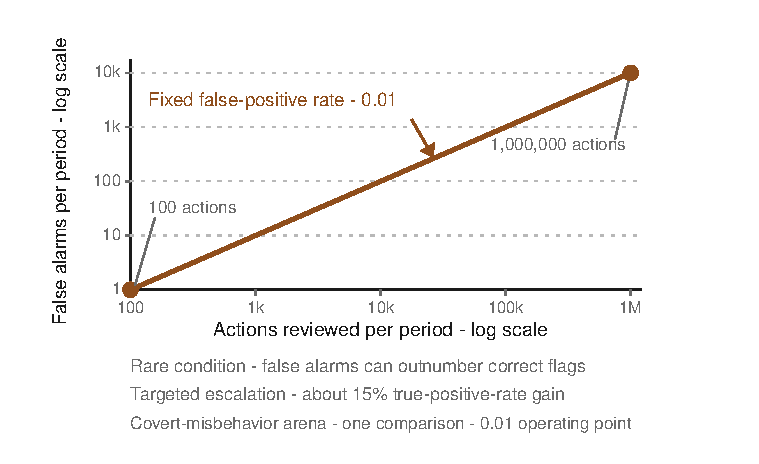
\includegraphics[keepaspectratio,alt={At fixed 0.01 false-positive rate, false alarms rise from 1 among 100 actions to 10,000 among 1,000,000 and can outnumber correct rare-event flags; targeted escalation adds about 15\% true-positive rate in one covert-misbehavior arena.}]{figures/ch15-queue-budget.pdf}}
\caption{At fixed 0.01 false-positive rate, false alarms rise from 1 among 100 actions to 10,000 among 1,000,000 and can outnumber correct rare-event flags; targeted escalation adds about 15\% true-positive rate in one covert-misbehavior arena.}
\end{figure}

False alarms scale with action volume and base rates. The approximately 15\% escalation gain comes from one covert-misbehavior-arena comparison at a 0.01 operating point.

Escalation is therefore a budgeted online decision. The system has to choose, as cases arrive, which uncertainty deserves scarce human attention now. That choice can account for expected consequence, novelty, reversibility, monitor disagreement, and the availability of a qualified owner. These inputs do not justify an opaque semantic risk formula. They define the evidence given to the judge and the explicit policy constraints applied to the queue.

My own orchestration fleet uses a related division of labor. Mechanical work proceeds autonomously, and judgments the system should not make unilaterally are collected in a structured morning decision ledger. The system does not silently resolve those entries. The design reserves interruptions for entries that need a person. I have not measured maintainer minutes, scrutiny depth, or escaped-defect rate, so the attention saving remains a design claim rather than a demonstrated outcome.

The associated wake-up contract makes the route more specific. The fleet should wake me for suspected wrong calls and for decisions about scope or trust. It should not wake me for passing runs or routine plumbing. A request has to state the outcome at stake, present a decision answerable in one line, list the options and the recommendation, and explain why the system cannot resolve the matter itself. The success criterion is behavioral. Engineers should not learn to filter the messages out.

This contract separates notification quality from verdict authority. A monitor may decide that a case meets the escalation rule. It should not quietly convert that classification into the substantive decision under review. The person named on the route must be able to reject the work, request evidence, narrow the scope, or authorize resumption. Naming an owner who cannot do these things assigns accountability without control.

The resumption state deserves explicit design, because asynchronous review creates races. If an agent continues acting while its escalation is pending, a later rejection may arrive after dependent actions have executed. If execution stops globally, an unrelated low-risk queue can be blocked by one ambiguous case. The route should state whether the affected action, trajectory, repository, or fleet pauses, which state is durable, and which decision token releases it.

Observed failure paths should determine checkpoint placement. When damaging actions become irreversible at deployment, a checkpoint after deployment can only document what happened. When the common failure begins as a plan silently expands its scope, waiting until the final diff makes reconstruction expensive. The companion pattern is narrow. Place human checkpoints where failure evidence shows that intervention can still change the outcome.

Human skill is another boundary. A reviewer who handles only rare anomalies may lose familiarity with ordinary system behavior, while automation inherits the routine cases that once maintained that familiarity. Bainbridge (\href{https://doi.org/10.1016/0005-1098(83)90046-8}{1983}) described this problem for industrial process control in ``Ironies of Automation.'' Its transfer to software-agent oversight is an analogy rather than a measured result on software work. It nevertheless identifies a design question that triage cannot answer alone. How will the person expected to intervene retain the knowledge needed to recognize and correct an abnormal state?

Xie et al.~(\href{https://arxiv.org/abs/2408.01703}{2024}) advanced a thinly supported companion proposal. Agent actions can be rendered as live state so that a reviewer inspects a trajectory before it terminates. The support is one prototype-scale item and does not establish improved oversight. The proposal is useful as a design prompt when late reconstruction has repeatedly failed, provided that the live view preserves the durable trace rather than replacing it.

Monitoring can alter the behavior it measures. An agent that knows it is being watched may adapt to the evaluation frame. I treat that possibility as a design caution and not as a measured result from Kale et al.~(2025), whose reported result was that monitor scaffolding mattered more than monitor awareness. In my own evaluation harnesses, I therefore use de-framed prompts that omit evaluation vocabulary, so the acting agent receives no cue to behave differently because it is being assessed. Removing that cue is a design precaution against one measurement effect, but it provides no proof that the resulting behavior matches unobserved production behavior.

Judge drift creates a second measurement problem. Deterministic rules drift when policy or event schemas change. Model judges drift when the evaluated distribution, the model version, or the rubric interpretation changes. Agent judges can drift most severely, because their behavior depends on a longer sequence of observations and actions. A monitor calibrated last quarter may preserve its interface while changing which cases reach humans.

Layering redistributes detection work, but it does not resolve who judges the judges. Human owners need sampled review of unflagged cases to estimate misses, adjudication of flagged cases to measure false alarms, and versioned records connecting each verdict to the monitor configuration that produced it. The sample cannot consist only of easy negatives. It has to include strata in which the monitor is likely to fail and cases drawn after relevant system changes. The sampling unit is the action or trajectory the monitor scored, and estimates from a stratified sample have to be weighted back to the deployed case mix before they describe the monitor in production.

These audits do not require blanket human oversight of every action. They require enough independent labels to estimate whether the chosen operating point still holds. When the estimate degrades, the response may be recalibration, a narrower deployment boundary, a new deterministic check, a rubric revision, or more human review. The correct response depends on the failure mechanism, and `use a stronger judge' is not a diagnosis.

\section{An operating protocol}\label{an-operating-protocol}

Start with one consequential agent workflow. Identify the acceptance decision that transfers authority from proposed work to an effect: merge, deploy, publish, modify data, contact a customer, or change another system's state. Name the person or role that owns that decision. When no one can be named, escalation cannot end in an accountable verdict.

For that workflow, list the claims a reviewer must establish before acceptance. Attach a falsification artifact to each claim where one is available: a test, a typed interface, a replay, a trace, a sandbox result, a policy match, or an executable example. Mark the claims that still depend on expert judgment. Do not count an explanation as evidence unless it makes one of those checks possible.

Measure the review path before adding friction. Record how long evidence takes to obtain, which tools or permissions it requires, where reviewers abandon the check, and which failures remain invisible after a green run. The objective is to find the cases in which the system charges a person for mechanical work or presents confidence without a reachable basis. No universal review-time target applies.

Place a forcing function at the accept decision for the cases in which shallow validation is plausible and consequential. Require an independent judgment or a claim-specific response before revealing the agent's recommendation. Preserve an explicit emergency bypass with an owner, a reason, an affected scope, and a follow-up state. Evaluate detection, delay, bypass, and workarounds together. Satisfaction alone will select for the gates that interfere least.

Build the monitor scaffold from exact checks outward. Use deterministic rules for exact policy violations, a model judge with a versioned rubric for contextual classification, and an agent judge only when sequential interpretation is necessary. Make every layer return the evidence a human needs to challenge it. Calibrate the stack against an expert-labeled stratified matched control set, choose and record the operating point, and translate the rates into expected queue volume at the actual base rate.

Define the escalation route as part of deployment. A flag should identify the decision owner, the outcome at stake, the evidence, the available options, the recommended action, the reason automation cannot decide, the state that is paused, and the event that resumes execution. Test the route by processing a real rejection through it. When the owner cannot stop or revise the action, assign authority before assigning accountability.

Sample both flagged and unflagged cases after deployment. Compare human verdicts with monitor decisions by risk stratum and monitor version. Recalibrate after material changes to agents, tools, rubrics, or workload, and examine whether awareness of monitoring changes behavior. Budget practice for the humans who must handle rare failures. A name in an escalation table does not preserve operational skill.

\section{Sources and evidence}\label{sources-and-evidence}

The evidence class and strength on each entry below come from its catalog record. Author-system cases in this chapter are narrative illustration and are not part of the evidence base.

\subsection{Building verification surfaces so verifying costs less than blind acceptance}\label{building-verification-surfaces-so-verifying-costs-less-than-blind-acceptance}

\begin{itemize}
\tightlist
\item
  lit/strong: Vasconcelos, H., Jörke, M., Grunde-McLaughlin, M., Gerstenberg, T., Bernstein, M., Krishna, R. (2022/2023). Explanations Can Reduce Overreliance on AI Systems During Decision-Making. PACM HCI 7(CSCW1). arXiv:2212.06823. Five experiments treat overreliance as a cost-benefit choice and find greater engagement when verification is cheaper or stakes are higher.
\item
  lit/directional: Fok, R., Weld, D.S. (2023/2024). In Search of Verifiability: Explanations Rarely Enable Complementary Performance in AI-Advised Decision Making. AI Magazine 45(3). arXiv:2305.07722. Across the XAI-reliance literature, explanations help only insofar as they enable verification.
\item
  Corroboration: the author's website, ``Two retrieval systems write this site'' (2026-06-10), an author-owned anecdotal account of schema-validated agent output landing as a git diff that serves as the review gate, and an unpublished internal record of the author's agent-workflow system. Both are narrative only and neither is an admitting basis. Dossier items corroborate only.
\end{itemize}

\subsection{Putting the forcing function at the accept decision, aimed at acceleration mode}\label{putting-the-forcing-function-at-the-accept-decision-aimed-at-acceleration-mode}

\begin{itemize}
\tightlist
\item
  lit/strong: Buçinca, Z., Malaya, M.B., Gajos, K.Z. (2021). To Trust or to Think: Cognitive Forcing Functions Can Reduce Overreliance on AI in AI-assisted Decision-making. PACM HCI 5(CSCW1), 188. arXiv:2102.09692. Cognitive forcing functions reduced overreliance where explanations failed (N=199).
\item
  lit/directional: Barke, S., James, M.B., Polikarpova, N. (2022/2023). Grounded Copilot: How Programmers Interact with Code-Generating Models. PACMPL 7(OOPSLA1). arXiv:2206.15000. Grounded theory from 20 programmers supports the suggestion-level acceleration/exploration split. Transfer to autonomous-agent diffs is untested. This directional item is the only source for the chapter's targeting rule.
\item
  Corroboration: none on record.
\end{itemize}

\subsection{Escalating only monitor-flagged cases to a human who owns the verdict, with a scaffolded monitor}\label{escalating-only-monitor-flagged-cases-to-a-human-who-owns-the-verdict-with-a-scaffolded-monitor}

\begin{itemize}
\tightlist
\item
  lit/strong: Kale, N., et al.~(2025). Reliable Weak-to-Strong Monitoring of LLM Agents. arXiv:2508.19461. Targeted escalation adds approximately 15\% TPR at FPR=0.01. Hybrid hierarchical-sequential scaffolds let weaker models monitor stronger agents. The paper reports that scaffolding mattered more than monitor awareness; the awareness caution in this chapter is my design caution, not a result from this paper. The setting is a covert-misbehavior arena, not production code review. This is the sole admitted evidence item for the whole grouping.
\item
  Corroboration: the author's website, ``Running my own agent city on Slack'' (2026-06-16), an author-owned anecdotal account of mechanical work proceeding autonomously while judgment calls accumulate in a decision ledger for a human; the author's website, ``WF2026: evals are the new CI'' field notes, an account distilled from other people's conference talks of a three-layer judge stack with a human owning the verdict; and unpublished internal context notes. None is an admitting basis. The conference-talk-derived account was demoted out of the evidence base and is not citable as independent support. The chapter's three-layer scaffold ordering rests on it and on nothing stronger. Dossier items corroborate only.
\end{itemize}

\subsection{Companion material carried in-text but not taught as a pattern}\label{companion-material-carried-in-text-but-not-taught-as-a-pattern}

\begin{itemize}
\tightlist
\item
  lit/strong: Rosbach, E., Ganz, J., Ammeling, J., Riener, A., Aubreville, M. (2024). Automation Bias in AI-Assisted Medical Decision-Making under Time Pressure in Computational Pathology. arXiv:2411.00998. This is the basis for the time-pressure paragraph. The setting is computational pathology, not software review.
\item
  lit/directional: Bainbridge, L. (1983). Ironies of Automation. Automatica 19(6), 775-779. \url{doi:10.1016/0005-1098(83)90046-8}. This is the single source behind the skill-retention paragraph. The evidence is pre-AI and industrial. Transfer to code review is analogical.
\item
  lit/anecdotal: Sarkar, A., et al.~(2022). What is it like to program with artificial intelligence? PPIG 2022. arXiv:2208.06213. This is the basis for the companion hypothesis that verification is the dominant cost. The magnitudes are not quantified.
\item
  lit/directional: Xie, L., Zheng, C., Xia, H., Qu, H., Zhu-Tian, C. (2024). WaitGPT: Monitoring and Steering Conversational LLM Agent in Data Analysis with On-the-Fly Code Visualization. UIST 2024. arXiv:2408.01703. This prototype-scale single item is the basis for the live-state proposal and the thinnest support in the chapter. Transfer to arbitrary code agents requires an operation-level abstraction that may not exist.
\item
  explorer/directional: DeepRare (Zhao 2026); Manager Agent (Masters 2025, arXiv:2510.02557); NIST AI RMF.
\item
  explorer/directional: Bounded Autonomy for Enterprise AI (Sohail 2026, arXiv:2604.14723).
\item
  explorer/directional: AMBIPOM human-LLM co-planning (He 2026, arXiv:2605.23023).
\item
  explorer/directional: Token Budgets (Khan 2026, arXiv:2606.04056). Together, the four explorer items support only the direction of the checkpoint-placement claim. None is strong.
\item
  Corroboration: an unpublished internal record of the author's repository-scale benchmark, an unpublished internal record of the author's background-agent review pipeline, and unpublished internal context notes corroborate the checkpoint-placement claim as narrative only. Dossier items corroborate only.
\end{itemize}

\subsection{Opening scene}\label{opening-scene}

\begin{itemize}
\tightlist
\item
  practitioner/corpus-verified: InfoQ, ``Stripe Engineers Deploy Minions, Autonomous Agents Producing Thousands of Pull Requests Weekly,'' 2026-03-20, \url{https://www.infoq.com/news/2026/03/stripe-autonomous-coding-agents/}. Reports over 1,300 production pull requests per week with human review retained. Carried as scale context; it reports no measure of review depth or defect escape.
\end{itemize}


\chapter{Autonomy calibration, provenance, effective gates, and accountability}
\label{ch16-autonomy-provenance-gates-accountability}
I built a human-approval queue to hold decisions an agent was not permitted to make. The architecture appeared conservative: the agent could prepare an action, but execution stopped at a human-only boundary.

An audit found paths around that boundary. Some scripts failed open when a required component was missing, and command construction reached execution without the validation the gate was supposed to enforce. The system could report that approval existed while allowing an action to bypass the person. The conservative appearance of the apparatus had concealed a material difference between policy and execution.

The chapter's four entries rest on seven evidence items, two of them strong. The accountability literature represented here consists largely of surveys, frameworks, and position papers, with one practitioner account and little production-grounded measurement. The practices are therefore testable defaults rather than universal policy; the entries on gate effectiveness and alignment between accountability and control have no strong supporting item.

The failed queue illustrates the broader problem. An autonomy policy constrains nothing unless the system enforces the boundary it names. A provenance label changes nothing unless it changes what a reviewer can learn or do. A human gate controls nothing unless the person can alter the execution path. An accountability assignment prevents nothing unless the named person has authority over the outcome.

These are separate design objects, but they fail in the same way when the operational path differs from the policy description.

Agent systems acquire more kinds of authority as they grow. One may restart a service, propose a migration, merge documentation, rotate a credential, or delete a branch. Calling the system ``autonomous'' collapses those different powers into one word. That word says nothing about reversibility, blast radius, available evidence, ownership of state, or the ability to interrupt execution.

\Needspace{5\baselineskip}

The useful unit is the transfer of control for one action class. Each transfer has:

\begin{itemize}
\tightlist
\item
  an initiator;
\item
  a proposed action;
\item
  an approving or executing party;
\item
  an artifact supporting the decision; and
\item
  a recorded outcome.
\end{itemize}

Once those elements are explicit, autonomy can be calibrated from observations, provenance can travel with the artifact, and the gate can be tested as an executable control. Accountability can then be assigned to a role that actually holds authority.

\hypertarget{widen-authority-one-action-class-at-a-time}{%
\section{Widen authority one action class at a time}\label{widen-authority-one-action-class-at-a-time}}

An autonomy ladder widens control one rung at a time for a defined action class. Each class keeps its own approval, modification, and outcome record. A \textbf{promotion threshold} is the criterion for moving that action to a wider rung.

One practitioner article, Priya C (\href{https://devops.com/when-should-a-devops-agent-act-without-human-approval/}{2026}), proposes roughly 95 percent unmodified approvals as a starting policy. It reports no measurement supporting that cutoff. The number has no claim to universality.

A team should instead define the performance difference that would justify wider authority, gather enough observations to detect that difference, and retain the underlying counts. The protocol here rests on one directional practitioner source and one strong controlled study concerning reviewer comprehension.

The ladder needs separate rails because action classes expose different risks. A service restart changes transient process state and can often be reversed with another restart. A credential rotation changes distributed configuration, invalidates clients, and may lock operators out of recovery. A branch deletion changes repository state. A proposed text edit changes only an artifact that still requires merge.

Hundreds of clean service restarts establish nothing about whether the same system can rotate credentials safely.

\begin{verbatim}
defined action class
    -> its own approval + modification + outcome record
        -> measured evidence
            -> widen authority one rung at a time

service restart rail              credential rotation rail
transient process state           distributed configuration
another restart may reverse       invalidates clients
clean restarts may widen rung     may block recovery access
        |                                  ^
        +-> establish nothing about -------+

permanent approval floor
    -> human authorization remains mandatory
    -> irreversible actions stay above
    -> high-blast-radius actions stay above

routine success does not remove the floor
\end{verbatim}

My operator policy makes this separation explicit. Service restarts are pre-approved. Destructive operations such as recursive deletion, force-push, and branch deletion require renewed confirmation every time. The policy is durable configuration, so a new session inherits the same boundary. This illustrates the shape of an action-specific policy; it is not evidence that these classifications suit another system.

\Needspace{5\baselineskip}

A transfer-of-control record documents every decision to let the system act, require approval, or return control to a person. For each action class, it should preserve:

\begin{itemize}
\tightlist
\item
  the proposed action;
\item
  the autonomy rung in force;
\item
  the reviewer's decision;
\item
  any human modification;
\item
  the observed outcome; and
\item
  later reversal or incident evidence.
\end{itemize}

Outcome correctness requires an action-specific definition. For a restart, ``the command exited zero'' is insufficient if the service never became healthy. For a patch, ``merged'' is insufficient if production failure caused an immediate revert.

Approval measures are proportions over repeated observations:

\begin{verbatim}
approval rate
    = approved proposals / reviewed proposals

unmodified approval rate
    = proposals approved without human change / reviewed proposals

modification rate
    = proposals changed by a human / reviewed proposals
\end{verbatim}

The denominators must refer to the same action class and autonomy rung. Combining restarts with schema changes can produce a stable aggregate while both underlying rates move in opposite directions. Excluding rejected or timed-out proposals makes the system look more acceptable by removing the transfers that failed. Recording only executed actions introduces survivorship bias because abandoned proposals disappear before the outcome record is built.

Part I established why an observed proportion is not the underlying property. Nine unmodified approvals among ten proposals and ninety among one hundred both produce 90 percent, but the first estimate is much less precise. The interval method depends on the analysis plan; the operational conclusion does not. A small-\(n\) percentage should not transfer authority merely because it crossed a displayed threshold.

The sampling unit also matters. A series of transfers reviewed by one person measures the reviewer-system pair as much as the system itself. A track record collected under one model version, prompt set, or harness revision describes that configuration. Changing any of them reopens the question the record was intended to settle.

Promotion also requires a power analysis. The team first defines the smallest change that would reverse the decision, such as the smallest increase in post-action failures that would make a wider rung unacceptable. It then estimates how many observations are needed to detect that change at the chosen error rates.

Rare, high-consequence failures may require more observations than the deployment can plausibly accumulate. In that case, the action cannot earn wider autonomy from its local record, even when every observed outcome has been clean.

Approval alone omits information captured by modification. A reviewer may approve every database query only after correcting its time window, tenant filter, or target environment. Approval is then 100 percent, even though autonomous execution would repeatedly reproduce a material error.

The modification record should retain what changed. Correcting punctuation and changing a production target have different implications. Modifications can be classified for analysis when the categories and inter-rater reliability procedure are fixed before the rates are examined.

Outcome correctness is a third measure because approval can reflect reviewer behavior rather than system quality. Reviewers under queue pressure may approve familiar actions quickly or reserve comments for severe defects. A rising unmodified approval rate combined with a rising rollback rate argues against promotion. Delayed outcomes must also remain attached to the original transfer, or failures discovered after the review window will be counted as successes.

Chen et al.~(\href{https://arxiv.org/abs/2507.08149}{2025}) complicate a capability-only account of automation. In their controlled study, limited understanding of agent behavior constrained willingness to adopt higher automation even as capability increased. Capability alone did not determine the limit.

\Needspace{5\baselineskip}

The verification surface is therefore part of the autonomy mechanism. A reviewer needs:

\begin{itemize}
\tightlist
\item
  a behavior summary;
\item
  the relevant artifact or diff;
\item
  the intended state transition;
\item
  the observed state transition; and
\item
  the evidence connecting the proposed action to the stated objective.
\end{itemize}

When those artifacts do not support comprehension, even an accurate system may fail to earn legitimate authority.

Comprehension should be tested at the rung under consideration. Ask reviewers to predict affected resources, identify the rollback path, and locate the evidence behind the system's claim before revealing the answer. Record where their understanding diverges from execution. No universal quiz score follows from this design.

The companion entry \texttt{require-comprehension-before-merge} makes the explain-back check explicit. An independent checker should evaluate the generating system's work.

Some action classes remain above a permanent approval floor, below which human authorization is never removed. Irreversible and high-blast-radius actions belong there when the consequence of a mistaken transfer exceeds what the observed record can justify. The floor is not a trust ramp and does not disappear after routine successes.

Least privilege should still constrain the executing identity so that a mistaken approval cannot authorize effects beyond the operation being reviewed.

Most teams should keep most consequential actions below full autonomy today because the supporting evidence remains thin and action-specific. The companion entry \texttt{set-autonomy-defaults-per-task-type} can initialize a policy table, but it cannot create a track record or replace the ladder.

\Needspace{5\baselineskip}

The executable decision is narrower:

\begin{enumerate}
\def\labelenumi{\arabic{enumi}.}
\tightlist
\item
  Define one action class.
\item
  Define a correct outcome and the material difference that would reverse the policy.
\item
  Record every proposed transfer, including rejection and timeout.
\item
  Estimate uncertainty.
\item
  Test reviewer comprehension.
\item
  Widen authority by one rung only when the observations support it.
\end{enumerate}

Two companion entries sit beside this practice. \texttt{measure-oversight-with-decomposed-metrics} separates overreliance from underreliance and classifies review interactions before counting coverage. The evidence for \texttt{attach-reliance-disclaimers} supports only its inclusion as a marked design option.

\hypertarget{put-provenance-where-review-happens}{%
\section{Put provenance where review happens}\label{put-provenance-where-review-happens}}

Tang et al.~(\href{https://arxiv.org/abs/2405.16081}{2024}) observed 28 developers in a laboratory study and found that they were unreliable at recognizing machine-generated code without assistance. When told that the code was generated, participants searched and verified more, and their repair performance improved. Cognitive workload also increased.

This study provides the strong evidence for provenance disclosure in this chapter. It used short code fragments under laboratory conditions.

A provenance label records how an artifact was produced and presents that record where the artifact is reviewed. It may be a pull-request label, a structured commit trailer, or an editor marker.

Recognition is the wrong task on which to spend reviewer attention. Machine-generated code has no stable visual signature. Asking reviewers to infer its origin consumes attention before they inspect its behavior and produces selective scrutiny: obvious generations receive extra review while plausible generations pass as ordinary work.

Attaching provenance at the review surface makes origin an input to the decision rather than a detection task.

The study suggests a specific mechanism. Disclosure caused participants to search and verify more, giving them additional evidence for repair. The label did not establish that the code was defective and performed no verification itself. Its value depended on the behavior it produced in a reviewer who had the tools and time to investigate.

A common misuse ignores that dependence. A warning badge can become a substitute for testing, as though declaring machine authorship discharged the maintainer's responsibility. It can also become a weak liability transfer in which the system announces risk while giving the reviewer no practical way to inspect it.

\Needspace{5\baselineskip}

A useful label connects to:

\begin{itemize}
\tightlist
\item
  the generation context;
\item
  the proposed diff or artifact;
\item
  the tests and verification results;
\item
  later human modifications; and
\item
  the role answerable for integration.
\end{itemize}

None of those artifacts is thereby proven correct.

The disclosure boundary needs a defined object. One pull request may contain human-written scaffolding, generated implementation, generated tests, and later human repairs. A request-level label is simple but loses that composition. A marker on every line is more precise but noisy and dependent on editor and diff support. Commit trailers provide a durable repository unit, although squashing, copying, and cherry-picking can detach the trailer from the code it described.

There is no universal granularity. The team should identify the review decision the label is meant to influence and choose the smallest unit whose provenance survives the repository workflow.

\Needspace{5\baselineskip}

Test that survival through:

\begin{itemize}
\tightlist
\item
  rebases;
\item
  cherry-picks;
\item
  squash merges;
\item
  file moves;
\item
  copied patches; and
\item
  partial adoption of generated work.
\end{itemize}

A provenance control that disappears during the ordinary merge path creates a confident but incomplete history.

My authorship-measurement project illustrates why provenance counts must remain narrow. I measured a 14.5 percent trailer-signed floor, a lower bound on visible trailer-marked authorship, because every detected trailer was treated as a true positive. The figure says nothing about total agent contribution and cannot be averaged with an inferred share.

A preregistered replication could not estimate the share of agent-authored code beyond commits carrying the trailer. I therefore discard the earlier exploratory range and report only the directly observed trailer-marked floor.

Provenance is also distinct from answerability. In my maintainer practice, an adoption pull request can preserve a contributor's commits while stating:

\begin{verbatim}
Supersedes #X
Credit: original fix by @X (commit preserved with original authorship)
\end{verbatim}

The original author remains attached to the work. The maintainer who adopts and submits it becomes answerable for the integration decision. Both facts survive in the artifact.

The format establishes attribution rather than correctness. It removes the need for a later reviewer to infer who produced the change and who accepted responsibility for putting it forward.

Persistent provenance also supports incident reconstruction. A reviewer investigating a regression can ask whether the failure arose during generation, human modification, integration, or a later environmental change. That distinction is harder when provenance exists only in an editor and disappears before merge.

The companion entry \texttt{record-steps-in-hash-chained-ledger} describes one tamper-evident history mechanism. The argument here does not depend on that implementation.

Tang et al.'s measured workload cost limits the recommendation. Increased cognitive effort may be acceptable when a marker directs attention to occasional generated work. In a codebase where nearly every change carries the label, constant exposure may tax reviewers and lose salience.

Large diffs, persistent queues, and experienced teams may respond differently over time. Local evaluation should therefore measure reviewer behavior and repair, not label coverage alone.

\Needspace{5\baselineskip}

Useful observations include whether reviewers:

\begin{itemize}
\tightlist
\item
  open referenced files;
\item
  inspect or run tests;
\item
  search documentation;
\item
  change the proposed code;
\item
  detect seeded defects; and
\item
  report excessive workload.
\end{itemize}

Compare equivalent review artifacts with and without disclosure under the actual tools and queue constraints. Using the same artifacts removes change difficulty from the comparison, as Chapter 1 recommends for paired designs.

\Needspace{5\baselineskip}

The experimental unit is the reviewer-artifact pair, not the artifact alone. The design must state:

\begin{itemize}
\tightlist
\item
  how reviewers are assigned to conditions;
\item
  whether any reviewer sees the same artifact twice;
\item
  how condition order is counterbalanced;
\item
  which defects count; and
\item
  how cognitive workload is measured.
\end{itemize}

The study provides no production threshold to copy.

If disclosure increases activity without improving repair, the marker may be producing ritual rather than evidence. If repair improves while queue delay or abandonment rises sharply, the team has found a real tradeoff between scrutiny and capacity. Either result is more useful than a policy requiring an ``AI-generated'' badge everywhere.

The relevant question is whether provenance changes verification in the deployed review environment.

The companion entry \texttt{write-an-agent-contribution-policy} covers repository rules for disclosure, attribution, and accepted contribution paths. A policy can standardize the wire format. It cannot make the marker effective. Effectiveness remains an observed relationship among the label, verification surface, reviewer behavior, and repair outcome.

\hypertarget{prove-that-a-gate-can-change-execution}{%
\section{Prove that a gate can change execution}\label{prove-that-a-gate-can-change-execution}}

Human gates have only directional support in this chapter and no strong evidence item. Sterz et al.~(\href{https://arxiv.org/abs/2404.04059}{2024}) propose an interdisciplinary framework for effective human oversight but provide no empirical validation of a universal test. Green (\href{https://arxiv.org/abs/2109.05067}{2022}) compared 41 government oversight policies with findings from human-computer interaction research and concluded that the human functions prescribed by those policies were generally not performable.

These sources justify an audit structure and a burden of proof. Whether a particular gate works remains unresolved until the deploying team tests it.

In a workflow diagram, the word ``gate'' implies causal control. In execution, an approval step may only record that someone clicked before an action the person and the click could not alter.

\textbf{Compliance theater} is a control whose visible form satisfies the policy description while its execution path does not mitigate the named risk. A \textbf{fail-open gate} stops enforcing its boundary when a dependency, validation step, or error path fails.

\Needspace{5\baselineskip}

The interdisciplinary framework identifies four conditions for effective oversight:

\begin{itemize}
\tightlist
\item
  \textbf{Causal power:} the person can stop or change the consequential action.
\item
  \textbf{Epistemic access:} the person can obtain the evidence needed to understand the decision before it takes effect.
\item
  \textbf{Self-control:} the person can exercise judgment rather than follow a compelled path.
\item
  \textbf{Fitting intentions:} the person intends and is prepared to perform the assigned oversight function.
\end{itemize}

Evaluate those conditions against an execution trace rather than the policy document. For every named gate, follow the proposed action through approval, mutation, dispatch, and durable state change. Inject the failures the gate claims to handle. Observe whether the reviewer receives the required evidence, whether rejection blocks every path, and whether a modified action requires renewed approval.

\begin{longtable}[]{@{}
  >{\raggedright\arraybackslash}p{(\columnwidth - 6\tabcolsep) * \real{0.2500}}
  >{\raggedright\arraybackslash}p{(\columnwidth - 6\tabcolsep) * \real{0.2500}}
  >{\raggedright\arraybackslash}p{(\columnwidth - 6\tabcolsep) * \real{0.2500}}
  >{\raggedright\arraybackslash}p{(\columnwidth - 6\tabcolsep) * \real{0.2500}}@{}}
\toprule\noalign{}
\begin{minipage}[b]{\linewidth}\raggedright
Condition
\end{minipage} & \begin{minipage}[b]{\linewidth}\raggedright
Question for the running gate
\end{minipage} & \begin{minipage}[b]{\linewidth}\raggedright
Observation to collect
\end{minipage} & \begin{minipage}[b]{\linewidth}\raggedright
Failure implication
\end{minipage} \\
\midrule\noalign{}
\endhead
\bottomrule\noalign{}
\endlastfoot
Causal power & Can the person stop or alter this exact action? & Rejection, cancellation, edit, and timeout traces & The click records assent but does not control execution \\
Epistemic access & Can the person inspect the relevant inputs, artifact, target, and consequences before deciding? & Missing context, inaccessible logs, and reconstruction errors & Approval rests on incomplete state \\
Self-control & Can the person decide without a forced default or impossible queue constraint? & Default acceptance, time pressure, and override use & The workflow substitutes acquiescence for judgment \\
Fitting intentions & Is the role expected and prepared to inspect the named risk? & Review actions, escalation behavior, and interviews & The role is ceremonial or aimed at another risk \\
\end{longtable}

The acceptance criteria must be system-specific. One team may require a deployment approver to cancel a queued release before the first production mutation and to see the exact artifact digest being deployed. Another may require a migration reviewer to revise the plan while withholding direct execution authority.

Name the claimed oversight function, build a trace capable of falsifying it, and decide in advance what observation would establish control.

Removing a dependency from a gate is itself a state change, so this failure test belongs in a contained environment. Chapter 7 supplies that boundary. Auditing a production gate by allowing its negative result to mutate production converts a test into an incident.

My approval queue failed this audit. Missing components allowed scripts to bypass the path that should have waited for a person. Unvalidated command construction weakened the connection between the reviewed proposal and the executed command. The existence of the queue did not establish causal power.

The failure is useful contrary evidence precisely because the queue was designed to preserve human-only decisions.

Another of my systems used a reproduction-before-mutation hook intended to require a reproducible failure before code could change. When a required binary was missing, the hook stopped enforcing the gate. The project documented the fail-open behavior rather than counting installation of the hook as coverage.

The case does not estimate how often gates fail this way. It shows how one environmental dependency can erase a governance boundary.

Mechanical and attentional gates fail differently.

A \textbf{mechanical gate} uses execution state to block an action until a condition holds, such as a verified signature or explicit \texttt{-\/-apply} flag. It may enforce a condition that does not establish the property for which the gate receives credit.

An \textbf{attentional gate} presents evidence to a person and requires a decision, such as review of a diff and its supporting checks. It may obtain a click without scrutiny.

Agent memory is neither. A remembered instruction has no independent causal path to enforcement.

My approval-gate configuration contains seven action-class rows. Each identifies the gate as mechanical or attentional, names an owner, and avoids reliance on agent memory. Mutating commands dry-run by default and require \texttt{-\/-apply}, placing a mechanical boundary between inspection and state change.

This is a design example, not evidence that seven rows, that flag name, or those classifications improve outcomes elsewhere.

More elaborate gates require the same audit. In pull request 1558 of my orchestration system, the review surface recorded:

\begin{verbatim}
Latest review attempt: 6
Quality score: 950/1000, threshold 850
\end{verbatim}

The attempt count and score are verified properties of that artifact. The gate was intended to concentrate human attention after repeated model review, and degradation of the gate was treated as an incident.

The claimed attention saving remains unmeasured because maintainer time, scrutiny depth, and escaped-defect rate were not recorded.

Optimizer and model-review gates depend on the same distinction. A threshold may mechanically block execution while providing no assurance that its score tracks the failure a person cares about. The companion entries \texttt{treat-objective-weights-as-reviewed-policy} and \texttt{gate-optimizer-output-behind-human-review} address those policy surfaces.

Their presence does not remove the need to test whether rejection changes system state and whether the reviewer can interrogate the score.

Green's analysis places the burden of proof on the institution deploying the automation. The team should justify why automation is appropriate for the action and demonstrate that reviewers can perform the function assigned to them.

When a reviewer cannot see the relevant evidence or cannot stop the action, attaching their name legitimizes the decision without reducing its risk. Accountability then moves toward the person with the least practical control.

That negative conclusion is bounded. Code review can offer unusually strong epistemic access because a reviewer can inspect an exact diff, run tests, examine history, and delay merge. Government-benefit decisions, live vehicle intervention, and repository changes do not create the same verification problem.

The gate must be tested in its own domain. These sources establish no universal conclusion about either human incapacity or human benefit.

Chapter 7 also showed why a control cannot be accepted merely because the harness reports that it ran. The governance extension asks whether a person can independently inspect the relevant state and interrupt the path that changes it. An override button without an independent signal provides nominal authority without usable control.

Three companion entries sit beside this practice: \texttt{separate-control-from-oversight}, \texttt{write-an-oversight-card}, and \texttt{keep-override-authority-real}. Each rests on one evidence item and can help distinguish control before action, observation after action, stated reviewer duties, and override paths.

None establishes that a particular gate works. That requires a trace showing that the reviewer had the evidence, authority, and execution path needed to change the outcome.

\hypertarget{assign-responsibility-only-where-control-exists}{%
\section{Assign responsibility only where control exists}\label{assign-responsibility-only-where-control-exists}}

Cavalcante Siebert et al.~(\href{https://arxiv.org/abs/2112.01298}{2023}) provide a conceptual bridge from responsibility theory to engineering practice: responsibility should be commensurate with the ability and authority to control an outcome. Suryana et al.~(2025) operationalized related questions in another domain through interviews with 103 users of partially automated driving systems, identifying gaps between expected and actual behavior and inconsistent adherence to operating protocols.

These are two directional literature items, and this practice has no strong supporting evidence item. Organizational-accountability research for agent systems is thin and recent. The sources support a defensible audit method. They provide no compliance threshold and no estimate of failure rates in software delivery.

After an incident, organizations often assign responsibility to the engineer who approved the action, monitored the system, or happened to be on call. That assignment may be administratively clear while remaining causally false. When the person lacked authority to halt the action, access to the relevant state, tools to change it, or time to intervene, responsibility has followed proximity rather than control.

The resulting responsibility gap produces blame without creating a path that could have prevented the failure.

\Needspace{5\baselineskip}

The control check begins before an incident. For every role named as accountable, identify the exact state transitions that role can:

\begin{itemize}
\tightlist
\item
  authorize;
\item
  alter;
\item
  stop; or
\item
  reverse.
\end{itemize}

Test those powers using the role's deployed identity rather than an administrator's demonstration. Record the information available at decision time, the tools through which intervention occurs, and the interval during which intervention remains effective.

Authority, access, tooling, and time are separate requirements. An engineer may have permission to cancel a deployment while lacking access to the tenant, model trace, or configuration needed to know that cancellation is warranted. A rollback command may exist while an irreversible external action commits before the reviewer has time to evaluate the evidence.

A role has control only when those elements combine into an effective intervention path.

\Needspace{5\baselineskip}

When responsibility exceeds control, the organization has two coherent options:

\begin{enumerate}
\def\labelenumi{\arabic{enumi}.}
\tightlist
\item
  Repair the role by granting the required authority, access, tooling, and time, subject to least privilege.
\item
  Move responsibility to the role that already holds those controls.
\end{enumerate}

Leaving the responsibility label in place while operational control remains elsewhere preserves the gap by design.

The check should include the identity that executes the action. In my enterprise data-access service, mutations are unavailable, requests use the caller's identity, and the audit log records that person. The agent cannot silently accumulate authority beyond what its operator already holds.

This design aligns execution and identity more closely than a shared privileged service account. Access justification and caller understanding remain separate checks.

\Needspace{5\baselineskip}

Identity passthrough also carries a cost. It improves attribution and limits silent privilege expansion, but it can reduce availability when the caller lacks a permission that a service account previously supplied. The system should first determine which authority the action genuinely requires, then measure:

\begin{itemize}
\tightlist
\item
  authorization failures;
\item
  escalation requests;
\item
  escalation completion time;
\item
  unauthorized access attempts; and
\item
  cases in which the agent requests authority broader than the task requires.
\end{itemize}

Provenance answers a neighboring but different question. It records who or what contributed to an artifact and how that contribution moved through the workflow. Accountability identifies the person or institution answerable for the decision to accept and deploy it.

The adoption pull-request format shown earlier preserves original authorship while transferring answerability for integration to the maintainer. Conflating the two roles would either erase contribution history or blame a contributor for a deployment decision they did not control.

The literature on meaningful human control offers two additional concepts: \textbf{tracking} and \textbf{tracing}.

Tracking asks whether system behavior follows the relevant and justified reasons or expectations of the people affected by it. Tracing asks whether a capable and aware person can be connected to the decision and its control path.

These concepts become operational only after the team translates them into observable behavior for its own system.

Suryana et al.~applied tracking and tracing through interviews with 103 users of Tesla Autopilot and Full Self-Driving features. The interviews revealed expectation-reality gaps and inconsistent adherence to operating protocols. This evidence comes from driving rather than software delivery; its transferable contribution is the interview method for revealing an operational control model different from the one described in design documents.

\Needspace{5\baselineskip}

For an agent that prepares production changes, a tracking interview might ask:

\begin{itemize}
\tightlist
\item
  What do users believe the agent may modify?
\item
  Which constraints do they expect it to preserve?
\item
  What evidence do they expect to stop execution?
\item
  When do they believe human approval is required?
\item
  What do they believe happens after rejection?
\end{itemize}

Those answers should be compared with policy and with actual execution traces.

\Needspace{5\baselineskip}

A tracing interview might ask:

\begin{itemize}
\tightlist
\item
  Who can explain this action?
\item
  Who could have changed or stopped it at each stage?
\item
  Which identity executed it?
\item
  Who could reverse it?
\item
  Where should a user escalate when behavior diverges?
\item
  What happens if that person is unavailable?
\end{itemize}

Compare the answers across operators, reviewers, system owners, and affected users. Inconsistent answers are evidence that the operational responsibility model is not shared.

The audit identifies distinct failures rather than producing one certification score. A shared credential may erase the responsible identity even when the system tracks user expectations well. A complete decision history may coexist with systematic misunderstanding about when the system will act. Combining both into one ``meaningful control'' score would hide the repair each problem requires.

\Needspace{5\baselineskip}

Operational definitions must therefore remain local. A deployment system may define a traceable decision through:

\begin{itemize}
\tightlist
\item
  the artifact digest;
\item
  approver identity;
\item
  execution identity;
\item
  target environment;
\item
  authorization token; and
\item
  rollback authority.
\end{itemize}

\Needspace{5\baselineskip}

A data-access agent may require:

\begin{itemize}
\tightlist
\item
  caller identity;
\item
  query purpose;
\item
  source authorization;
\item
  returned-field records; and
\item
  a durable record of disclosure.
\end{itemize}

A partially automated vehicle has different timing, embodiment, and safety constraints. The questions about authority, awareness, and intervention transfer across domains. The measured rates and exact controls do not.

Collective work complicates responsibility without removing it. Models propose actions, tools execute them, reviewers approve them, platform teams configure permissions, and managers allocate review capacity. The companion entry \texttt{rebuild-collective-accountability} addresses how those contributions form an institutional account, while \texttt{scale-review-capacity-to-experience} addresses review planning by contributor experience.

Neither should diffuse answerability so widely that no role owns a state transition it can actually stop.

\hypertarget{audit-the-path-from-policy-to-execution}{%
\section{Audit the path from policy to execution}\label{audit-the-path-from-policy-to-execution}}

Run four checks against one defined action class and one real repository workflow.

\hypertarget{test-the-autonomy-transfer}{%
\section{Test the autonomy transfer}\label{test-the-autonomy-transfer}}

\Needspace{5\baselineskip}

Define:

\begin{itemize}
\tightlist
\item
  the action class;
\item
  the current autonomy rung;
\item
  a correct outcome;
\item
  the material difference that would justify wider authority; and
\item
  the failures that would prevent promotion.
\end{itemize}

Record every proposed transfer, including rejected, modified, timed-out, abandoned, and executed proposals. Do not combine action classes or autonomy rungs, and do not build the record from executed actions alone.

Calculate uncertainty around approval, modification, and outcome rates. Test whether reviewers understand the affected state, evidence, and rollback path. Widen authority by one rung only when those observations support the change.

\hypertarget{test-whether-provenance-survives-review-and-integration}{%
\section{Test whether provenance survives review and integration}\label{test-whether-provenance-survives-review-and-integration}}

Choose the smallest provenance unit that can survive the repository workflow while still representing the review decision it is intended to affect.

\Needspace{5\baselineskip}

Exercise that marker through:

\begin{itemize}
\tightlist
\item
  rebases;
\item
  cherry-picks;
\item
  squash merges;
\item
  file moves;
\item
  copied patches;
\item
  partial adoption; and
\item
  later human modification.
\end{itemize}

Verify that a reviewer can distinguish generation, human revision, and integration responsibility after each transformation.

Keep the count semantics narrow. The 14.5 percent trailer-signed floor described earlier is a lower bound on visible trailer-marked authorship. It must not be combined with an inferred contribution share.

\hypertarget{test-the-gate-as-a-failure-experiment}{%
\section{Test the gate as a failure experiment}\label{test-the-gate-as-a-failure-experiment}}

Run the gate audit in a contained environment. Name the action, gate, and decision owner, then capture the complete execution trace.

\Needspace{5\baselineskip}

Remove or fail each gate dependency in turn. Exercise:

\begin{itemize}
\tightlist
\item
  approval;
\item
  rejection;
\item
  modification;
\item
  cancellation;
\item
  timeout;
\item
  missing validation;
\item
  missing binaries or services;
\item
  stale approval tokens; and
\item
  attempts to execute through alternate paths.
\end{itemize}

Inspect the evidence available to the reviewer and verify the durable state produced by each decision. A rejected action must fail to execute through every path. A modified action must receive renewed review when the modification changes the authorized state transition.

Interview the assigned reviewer about the risk they believe they are checking, then compare that account with the actual execution path. Repair or remove a gate that cannot demonstrate causal power and epistemic access. Decide explicitly how queue pressure, defaults, incentives, and emergency procedures will preserve self-control and fitting intentions.

\hypertarget{audit-accountability-in-two-passes}{%
\section{Audit accountability in two passes}\label{audit-accountability-in-two-passes}}

\hypertarget{pass-one-verify-operational-control}{%
\paragraph{Pass one: verify operational control}\label{pass-one-verify-operational-control}}

For each role named as accountable, select a real action and test the role's deployed permissions.

\Needspace{5\baselineskip}

Exercise whether the role can:

\begin{itemize}
\tightlist
\item
  reject the action;
\item
  alter its scope;
\item
  stop execution;
\item
  inspect the relevant evidence;
\item
  initiate recovery; and
\item
  reverse the result where reversal is part of the claimed control.
\end{itemize}

Record the state transitions outside that role's authority, the information it cannot access, the tools it lacks, and the point after which intervention becomes ineffective.

Where control is missing, either repair the role within least-privilege constraints or reassign responsibility to the role that holds the necessary authority.

\hypertarget{pass-two-compare-the-stated-and-experienced-control-models}{%
\paragraph{Pass two: compare the stated and experienced control models}\label{pass-two-compare-the-stated-and-experienced-control-models}}

Interview actual users, operators, reviewers, and owners using tracking and tracing questions. Compare their justified expectations with policy and execution traces.

\Needspace{5\baselineskip}

Record as separate findings:

\begin{itemize}
\tightlist
\item
  expectation mismatches;
\item
  protocol deviations;
\item
  actions without a traceable execution identity;
\item
  reviewers who cannot explain the decision they approved;
\item
  roles assigned responsibility without intervention power;
\item
  ineffective escalation routes; and
\item
  delays that allowed the action to become irreversible before review.
\end{itemize}

Repeat the first pass whenever permissions, action classes, execution paths, or recovery mechanisms change. Repeat the second when the user population, operating protocol, interface, or escalation policy changes.

\Needspace{5\baselineskip}

Measure the findings that carry operational weight, such as:

\begin{itemize}
\tightlist
\item
  untraceable actions;
\item
  failed stops;
\item
  unauthorized execution paths;
\item
  expectation mismatches;
\item
  dead-end escalations;
\item
  stale approvals;
\item
  interventions that arrive too late; and
\item
  time lost before someone with effective control becomes involved.
\end{itemize}

Do not adopt a pass rate borrowed from another system. Decide in advance which failures invalidate the accountability claim and preserve the identities, traces, interviews, and execution evidence required to reproduce that decision.

\section*{Sources and evidence}

Support is thin across the chapter: four developed practices carry seven evidence items, of which two are strong and five directional; six are scholarly sources and one is a practitioner source. \texttt{audit-human-gates-for-effectiveness} and \texttt{align-accountability-with-actual-control} carry no strong evidence item.

\textbf{graduate-autonomy-per-action-track-record}

\begin{itemize}
\tightlist
\item
  Directional evidence: ``When Should a DevOps Agent Act Without Human Approval?'', Bala Priya C, DevOps.com, 2026-05-11, \href{https://devops.com/when-should-a-devops-agent-act-without-human-approval/}{article}. Supports action-type autonomy promotion at roughly 95\% unmodified approval, permanent approval floors for irreversible or high-blast-radius actions, and decision-ready gates with timeout plans. The protocol comes from one practitioner article; the threshold is stated, not measured.
\item
  Strong evidence: Chen, V., Talwalkar, A., Brennan, R., Neubig, G. (2025). Code with Me or for Me? How Increasing AI Automation Transforms Developer Workflows. arXiv:2507.08149. In the controlled study, users' failure to understand agent behavior, not capability, limited broader adoption.
\item
  Corroboration (narrative only): a demoted author-distilled field note about a 2025 lights-off agent factory failure, the operator policy, and an essay describing per-action autonomy with a batched morning decision ledger. The field note is not independent support.
\end{itemize}

\textbf{label-ai-provenance}

\begin{itemize}
\tightlist
\item
  Strong evidence: Tang, N., Chen, M., Ning, Z., Bansal, A., Huang, Y., McMillan, C., Li, T. J.-J. (2024). A Study on Developer Behaviors for Validating and Repairing LLM-Generated Code Using Eye Tracking and IDE Actions. arXiv:2405.16081. Supports improved repair performance and greater verification effort with provenance disclosure; recognition without disclosure was unreliable. Limited by a small laboratory sample and code chunks of tens of lines; the attention cost may not scale to constant exposure.
\item
  Corroboration: none on record.
\end{itemize}

\textbf{audit-human-gates-for-effectiveness}

\begin{itemize}
\tightlist
\item
  Directional evidence: Sterz, S., et al.~(2024). On the Quest for Effectiveness in Human Oversight: Interdisciplinary Perspectives. ACM FAccT 2024. arXiv:2404.04059. Supports four conditions for effective oversight persons; gates failing any condition are compliance theater. The framework is motivated by EU AI Act Article 14, not empirically validated.
\item
  Directional evidence: Green, B. (2022). The Flaws of Policies Requiring Human Oversight of Government Algorithms. Computer Law \& Security Review 45, 105681. arXiv:2109.05067. Compares 41 policies with the human-computer interaction record and shifts the burden of proof to the deploying institution. The negative claim transfers only where reviewers lack real verification surfaces; code review differs in verifiability.
\item
  Corroboration (narrative only, contrary): the human-approval queue audit found fail-open scripts and unvalidated command construction, while the reproduction-before-mutation hook stops enforcing when a required binary is absent.
\end{itemize}

\textbf{align-accountability-with-actual-control}

\begin{itemize}
\tightlist
\item
  Directional evidence: Cavalcante Siebert, L., et al.~(2023). Meaningful human control: actionable properties for AI system development. AI and Ethics 3, 241-255. arXiv:2112.01298. Supports responsibility commensurate with ability and authority to control, the framework's third actionable property.
\item
  Directional evidence: Suryana, L. E., Nordhoff, S., Calvert, S., Zgonnikov, A., van Arem, B. (2025). Meaningful human control of partially automated driving systems: Insights from interviews with Tesla users. Transportation Research Part F 113, 213-236. Applies tracking and tracing criteria to 103 users to localize expectation-reality gaps and inconsistent protocol adherence. The method requires case-specific operationalization, yields failure localization rather than a compliance score, and is evidenced here in the driving domain. No arXiv identifier or DOI is carried in the catalog record, so the inline citation is unlinked.
\end{itemize}


\part{Work allocation and cost engineering}

\chapter{Agent topology selection and dynamic task allocation}
\label{ch17-agent-topology-dynamic-task-allocation}
In one CodeProbe rerun (\href{https://github.com/sjarmak/codeprobe}{public repository}), I changed an agent's preamble to correct a retrieval behavior I had already diagnosed. The patch reduced cost while leaving the motivating failure intact.

On the affected task family, cost fell by 28 percent, while the primary reward difference was +0.0048 with a t statistic of 0.27, indistinguishable from noise in that comparison. The wall-clock prediction failed in both direction and magnitude. I had predicted a 40 percent reduction, but elapsed time increased by 3.9 percent. The agent still accepted a false-negative retrieval result and constructed its answer around missing evidence.

The patch changed the wrong variable. The preamble instructed the agent to synthesize for coverage, but the execution path still treated an empty tool result as authoritative. That coupling belonged to the harness rather than to the sentence-level wording of the prompt.

Prompt changes are cheap, visible, and easy to isolate in an experiment. Structural changes alter component boundaries: which worker retrieves evidence, which worker interprets it, what crosses the handoff, and which component can reject the result. They are more expensive to implement and harder to evaluate because several causal paths may move together. They are also sometimes the only intervention aimed at the point where the failure is produced.

\section{Move from prompt changes to structural repair only after persistence}\label{move-from-prompt-changes-to-structural-repair-only-after-persistence}

A failure class does not become persistent merely because it occurred more than once. I call a class persistent only after a paired comparison across model versions, with repeated trials, shows that it survives. One successful run on the newer model proves no more than one failed run on the older one.

Chapter 1's variance discipline still applies when the proposed treatment is a model upgrade. Analyze paired per-item differences rather than comparing two aggregate scores.

Once persistence is established, Chapter 10's taxonomy and first-upstream-failure method locate the earliest supported cause. That location constrains the repair. If retrieval produced an incomplete candidate set, adding a stronger instruction for the final writer to cite sources attacks the last visible symptom. The relevant repair belongs where the candidate set is formed, checked, or handed off.

The companion catalog states the broader rule as repairing the supported root cause rather than the final visible error. Its evidence is thin, so I use it here only as a diagnostic reminder.

Cemri et al.~(\href{https://arxiv.org/abs/2503.13657}{2025}) developed MAST, a taxonomy of failures in multi-agent language-model systems. They reported limited gains from prompt improvements on persistent classes and stronger results from interventions such as redesigned verification topology and modular roles while retaining the same underlying model.

The evaluated systems included benchmark frameworks such as AG2 and ChatDev rather than production deployments. The findings therefore establish plausible structural interventions within those frameworks, not portable recipes for arbitrary agent systems.

Kim et al.~(\href{https://arxiv.org/abs/2602.09937}{2026}) provide a stronger cross-version result in another domain. Across the capability tiers evaluated in OpenRCA, dominant failure modes in cloud root-cause analysis remained present. Prompt engineering did not eliminate communication failures, while richer communication protocols reduced them by as much as 15 percentage points.

That is evidence that an architectural failure can survive a more capable model. It does not establish a coding-agent failure rate or show that prompt engineering is generally ineffective.

The OpenRCA result separates two failure mechanisms. Protocol enrichment addressed communication failures, whereas hallucinated interpretation required another intervention. A structured handoff cannot repair a worker that invents the meaning of accurate evidence, and a stronger verifier cannot recover evidence no upstream component retrieved.

``Change the structure'' is therefore not a remedy. It is an instruction to revisit the causal boundary that produced the observed class.

A \textbf{multi-agent system} consists of several model-driven workers coordinating on one task. Its \textbf{topology} determines which workers exchange observations, where decisions converge, and which component owns shared state. Topology is distinct from implementation. Two programs can use the same queue library while exposing different communication structures, and two runtimes can implement the same topology.

Role specialization is one possible structural intervention. It assigns workers different responsibilities, evidence access, and acceptance conditions instead of asking each worker to perform the complete task.

In the opening retrieval case, specialization could separate candidate discovery from evidence adjudication. The retrieval worker would return candidates together with explicit coverage information. An adjudicator would decide whether an empty result supported a negative conclusion before the writer could treat absence of results as absence of evidence.

The specialization is justified only because it creates a boundary at which the false-negative claim becomes visible and rejectable. Adding personas without changing evidence or authority does nothing.

Structured handoffs can address the same coupling:

\begin{verbatim}
query: exact request issued to the retriever
candidates: identifiers returned
coverage_checks: alternate queries and their results
claim: sender's interpretation
status: supported | incomplete | failed
\end{verbatim}

The schema does not make the interpretation correct. It keeps evidence, interpretation, and completion status separate. An incomplete search can no longer become indistinguishable from a supported negative result unless another component explicitly makes that conversion.

During failure, the status must remain \texttt{failed} or \texttt{incomplete}. Converting it to an empty success recreates the original defect behind a cleaner interface.

\Needspace{5\baselineskip}

The structural boundary may also be a verification loop rather than another worker. One agent can produce an artifact, run a deterministic check, inspect the failure, and revise. An independent reviewer becomes useful when:

\begin{itemize}
\tightlist
\item
  the producer is poorly positioned to detect its own mistake;
\item
  the reviewer needs independent evidence access;
\item
  verification policy should remain isolated from generation; or
\item
  the consequence warrants a separate decision owner.
\end{itemize}

Role specialization describes distinct responsibilities, not necessarily distinct model instances.

The first structural question is therefore:

\begin{quote}
Which decision requires an independent state or authority boundary?
\end{quote}

The number of agents follows from that answer. Sometimes no additional worker is needed. Sometimes one verifier is enough. Five workers sharing the same incomplete evidence can amplify confidence without changing the failure path.

Accounts grouped under ``harness engineering'' describe teams accumulating capability in execution boundaries, verification loops, repository instructions, rollback paths, and approval controls rather than in prompts alone. Böckeler (\href{https://martinfowler.com/articles/exploring-gen-ai/harness-engineering.html}{2026}) analyzes vendor-reported practice from the OpenAI Codex team. Jain (\href{https://www.reddit.com/r/devops/comments/1touxz4/}{2026}) writes from practitioner experience rather than a controlled evaluation.

Neither source supplies enough verification detail to estimate an effect. They describe where practitioners report making repairs. Cemri et al.~and Kim et al.~carry the evidentiary claim that some persistent classes responded to structural intervention.

My trace data adds a caution about what prompt evidence can establish. Across 1,705 visible thinking blocks from 199 traces, agents never named the two dominant tools in their written reasoning. Sixty-five explicit intentions to find references produced no use of the purpose-built reference tool.

Zero mentions did not imply zero prompt influence. In a later 17-run experiment, deliberation-style preambles changed tool selection on matching tasks while scores remained 4.0 versus 4.0.

These observations separate two effects. Prompt steering may improve selection efficiency without improving task success. The target retrieval failure in my rerun still survived. Another wording change was therefore not the primary repair. The system needed a boundary that checked retrieval coverage before synthesis trusted the result.

\Needspace{5\baselineskip}

Structural repair carries costs. Splitting work introduces:

\begin{itemize}
\tightlist
\item
  handoff failures;
\item
  additional tokens and latency;
\item
  more state identities;
\item
  more opportunities for stale or conflicting evidence;
\item
  false rejection by verifiers; and
\item
  loss of context at specialist boundaries.
\end{itemize}

A protocol may omit the field later needed for diagnosis, while a specialist may lose information a generalist would have retained. Representing topology in configuration may make revision easier, but that companion proposal has thin support and an unmeasured maintenance burden.

\Needspace{5\baselineskip}

The repair criterion is causal and comparative:

\begin{enumerate}
\def\labelenumi{\arabic{enumi}.}
\tightlist
\item
  Change the smallest boundary capable of interrupting the observed failure path.
\item
  Preserve the failure evidence through that boundary.
\item
  Replay the same cases under paired repeated trials.
\item
  Measure whether the target class moved.
\item
  Inspect which new classes appeared.
\end{enumerate}

If the class does not change, the new structure added coordination without repairing the cause.

\section{Require fan-out to beat the live single-agent baseline}\label{require-fan-out-to-beat-the-live-single-agent-baseline}

Every proposal to add debate, delegation, or parallel workers needs a live single-agent control.

\textbf{Fan-out} assigns one task, or parts of it, to several workers whose outputs must later be selected or combined. \textbf{Delegation} transfers responsibility for a defined unit of work to another worker. Neither mechanism deserves credit merely because the configuration makes it available.

The golden set from Chapter 4 supplies the comparison. Replay the current single-agent workflow and the proposed team on the same versioned tasks and executable oracles. Record the promotion rule before the first run. Use the same number of repeated trials in both arms and score reliability through pass\textsuperscript{k} where that metric matches the deployment semantics.

The multi-agent treatment advances only when it clears both the success requirement and the relevant cost limit. Chapter 2's Pareto discipline rejects a quality gain whose operating cost makes the workflow unusable.

The gate does not presume that fan-out will fail. Work with independent branches, high error costs, or reasoning demands beyond one reliable trajectory may clear it. Those properties make fan-out plausible. They do not remove the need to measure whether coordination and aggregation consume the expected benefit.

Chun et al.~(\href{https://arxiv.org/abs/2503.12029}{2025}) compared debate configurations with task baselines and reported the inference cost of the debate variants themselves. They did not compare debate with a single-model baseline on cost and identified that comparison as an open question. Debate therefore receives no presumed efficiency benefit.

Li et al.~(\href{https://arxiv.org/abs/2606.00655}{2026}) provide a controlled cost result from SIMAS. Their multi-agent configurations used roughly 15 times as many tokens, returns were non-monotonic as agents were added, and debate sometimes underperformed self-correction.

These are strong results within the tested tasks and configurations. They do not supply a universal exchange rate for another worker. Token premiums depend on prompt length, number of rounds, context sharing, model mix, and duplicated work.

A strong source synthesis across several studies supports the general need for a gate, but no standardized experiment settles it. Other directional syntheses cover heterogeneous and homogeneous teams, consensus systems, and scaling networks: Tian et al.~(\href{https://arxiv.org/abs/2509.23537}{2025}), Kumar et al.~(\href{https://arxiv.org/abs/2604.13120}{2026}), Bertalani\v{c} et al.~(\href{https://arxiv.org/abs/2605.00914}{2026}), and Qian et al.~(\href{https://arxiv.org/abs/2406.07155}{2024}).

Because those syntheses overlap in their underlying sources and were not retained as strong controlled evidence, I use them only for direction. The operational decision still comes from reproducing the comparison on the target workload.

Aggregation belongs inside the treatment definition. Chapter 5 described an exploratory plurality-vote oracle gap of up to 32.3 percentage points from Bertalani\v{c} et al.~A correct answer existed among the candidates, but the vote selected another answer. That establishes a failure mode rather than its frequency elsewhere.

\Needspace{5\baselineskip}

It is enough to separate two outcomes:

\begin{itemize}
\tightlist
\item
  at least one worker produced a correct candidate; and
\item
  the system returned the correct candidate.
\end{itemize}

Suppose five workers review a code change. Three repeat the same shallow diagnosis, one identifies a real race condition, and one reports an unrelated issue. Plurality voting selects the shallow diagnosis even though the candidate set contains the critical finding.

\Needspace{5\baselineskip}

A synthesis worker may recover the minority report, but it can also suppress it when all findings arrive as undifferentiated prose. The evaluation must therefore:

\begin{itemize}
\tightlist
\item
  score the final system output;
\item
  retain candidate-level results;
\item
  record the aggregation decision; and
\item
  report whether the aggregator discarded an oracle-correct candidate.
\end{itemize}

The same requirement applies to debate. Later turns can make workers converge by exposing them to one early answer even when independent reasoning never resolves the problem. If independent judgment is the reason for adding reviewers, the treatment must preserve that independence long enough to test it.

Blind review lanes, in which reviewers do not see the producing worker's identity or conclusion, are a thinly supported companion option. They reduce one obvious coupling path but are not an established remedy for correlated errors.

\Needspace{5\baselineskip}

Cost measurement must include the full topology:

\begin{itemize}
\tightlist
\item
  planner input and output;
\item
  worker context and generation;
\item
  inter-worker messages;
\item
  retries;
\item
  failed branches;
\item
  synthesis;
\item
  verification; and
\item
  the final response.
\end{itemize}

Measure latency separately from total computation. Parallel execution may reduce wall-clock time while increasing tokens and monetary cost. That trade may be justified for a high-consequence incident and unacceptable for routine maintenance.

Chapter 18 develops routing and cost engineering in more detail. The minimum requirement here is to choose the cost axis that matters, measure it end to end, and record the acceptable increase before seeing the treatment result. A ceiling selected afterward can always be adjusted to preserve the favored architecture.

One validity check comes before any outcome comparison: the multi-agent mechanism must actually execute.

In my repository-scale benchmark, I configured a lean-subagent treatment across four arms and roughly 200 trials, including investigation tasks, and observed zero subagent spawns. The result showed that the treatment never entered the causal path. It did not show that subagents were ineffective.

Configuration is not behavior. A system may expose a delegation tool while the planner never invokes it. It may dispatch workers and ignore their responses. It may ask several workers questions that do not meaningfully partition the task. All can be labeled ``multi-agent'' while operating as an effectively single-agent system.

\Needspace{5\baselineskip}

I therefore instrument the treatment at three levels:

\begin{enumerate}
\def\labelenumi{\arabic{enumi}.}
\tightlist
\item
  \textbf{Configuration:} which topology and tools were available.
\item
  \textbf{Execution:} delegations, messages, worker completions, retries, and aggregation decisions.
\item
  \textbf{Outcome:} how those events contributed to the final result and cost.
\end{enumerate}

A run enters the multi-agent comparison only when the trace shows that the defining coordination behavior occurred.

That eligibility rule must be declared before execution. Writing it afterward selects runs based on observed behavior or outcome. Declared in advance, it distinguishes noncompliance from architectural failure.

\Needspace{5\baselineskip}

The distinction guides diagnosis:

\begin{itemize}
\tightlist
\item
  No delegation means the planner or tool boundary failed to activate the treatment.
\item
  Useful branches discarded by aggregation indicate a convergence failure.
\item
  Identical branch errors from shared context indicate a common upstream dependency.
\item
  Divergent correct candidates with a wrong final answer indicate a selection failure.
\item
  Expensive duplicate work with no gain indicates a decomposition failure.
\end{itemize}

The single-agent baseline must remain live as models change. A topology that once improved performance may become unnecessary when a stronger model absorbs the relevant capability. It may also become more valuable when the stronger model becomes a better planner while specialists remain inexpensive.

Replaying both configurations for each consequential release turns that shift into a measured comparison. Without the single-agent arm, improving team scores may conceal that the simpler system improved faster.

A compact promotion record can contain:

\begin{verbatim}
golden_set_version: repository-maintenance-2026-07

single_agent:
  pass^k:
  total_tokens:
  elapsed_time:
  failures_by_class:

multi_agent:
  pass^k:
  total_tokens:
  elapsed_time:
  failures_by_class:

mechanism_check:
  delegations_observed:
  branches_consumed:
  aggregator_used:

aggregation_check:
  correct_candidates_retained_or_discarded:

promotion_rule:
  success_floor:
  cost_ceiling:

decision:
  promote | retain baseline | redesign treatment
\end{verbatim}

This gate answers whether to divide the work. Topology selection answers how. A multi-agent design that cannot clear the gate should return to structural diagnosis. The next experiment may require a narrower specialist boundary, a different aggregator, or no additional worker.

\section{Choose topology by task shape and fault propagation}\label{choose-topology-by-task-shape-and-fault-propagation}

Jia et al.~(\href{https://arxiv.org/abs/2602.19843}{2026}) injected synthetic faults into three multi-agent architectures in MAS-FIRE. Closed-loop architectures neutralized more than 40 percent of faults that caused the linear pipeline to collapse, and stronger foundation models did not uniformly produce greater robustness.

The faults were synthetic and the comparison covered three architectures. The result does not establish a general preference for closed loops. It does show that message routes and feedback paths can determine whether a local error remains local or becomes a system failure.

A \textbf{pipeline} passes work through a fixed sequence of stages. It fits tasks that decompose into stable ordered transformations, such as:

\begin{verbatim}
retrieve candidate files
    -> extract relevant regions
        -> generate patch
            -> run tests
\end{verbatim}

Its advantage is inspectability. State moves in one direction, and each transition has a defined producer and consumer. Its weakness is the same property. An early omission can flow through every later stage without any component returning to the source.

Pipelines also compress meaning at each handoff. If retrieval emits only file excerpts, the patch stage may never learn that coverage was uncertain. A status field can preserve that uncertainty, but it does not create a return route. When downstream evidence can invalidate an upstream decision, the task no longer has a purely linear structure even if its implementation remains a sequence of functions.

An \textbf{orchestrator-worker topology} assigns one component responsibility for planning, dispatch, and integration while workers perform bounded tasks. It fits work whose decomposition depends on the initial state but whose branches can be evaluated separately.

A repository migration may require the orchestrator to identify affected packages, send independent compatibility checks to workers, and combine the findings into an ordered plan.

The orchestrator owns global task state. Workers should receive enough evidence for their assignments without inheriting the complete history by default. Their outputs return through a defined convergence point where conflicts and missing work can be detected.

Failure of the orchestrator has a larger blast radius than failure of one worker. Durable state, stable identities, and replay at that boundary therefore matter more to reliability than adding another worker.

A \textbf{hierarchy} or explicit leadership structure extends this arrangement when a flat team would exchange too many messages or when subproblems require their own coordination. A lead assigns work to subordinate groups and accepts bounded summaries rather than allowing every worker to communicate with every other worker.

This can reduce message growth. It also introduces information loss and concentrates authority. A hierarchy earns its cost only when the lead measurably reduces communication and integration burden without suppressing critical evidence. Titles assigned to the agents establish nothing.

A \textbf{blackboard} is shared evolving state that workers read and update. It fits tasks whose next useful action depends on discoveries made by any participant, such as an incident investigation in which logs, hypotheses, eliminated causes, and requested checks change throughout the run.

The blackboard externalizes state that would otherwise be scattered across pairwise conversations. It also creates concurrency obligations. Updates require identities, versions, conflict rules, provenance, and a distinction between an untested hypothesis and an established observation.

\Needspace{5\baselineskip}

Consider a security review of a large change:

\begin{itemize}
\tightlist
\item
  A pipeline fits fixed analyzers followed by one synthesis step.
\item
  An orchestrator-worker design fits a planner dividing the diff by attack surface and assigning bounded reviews.
\item
  A hierarchy becomes plausible when package leads coordinate their own specialist groups.
\item
  A blackboard fits an exploratory investigation in which one discovery should redirect every other reviewer.
\end{itemize}

These topologies can be combined. An orchestrator may dispatch pipelines. A hierarchy may use a blackboard for cross-group evidence while keeping control messages within leadership paths.

The relevant architectural properties are ownership of each state transition and the participants able to observe, challenge, or revise it; a configuration label alone does not establish either property.

Zhao et al.~(\href{https://arxiv.org/abs/2605.26178}{2026}) provide strong experimental evidence from ATOM that topology is a first-order variable and that adapting it to task difficulty can outperform one average design. Their evaluation used five-agent teams with two open models across MMLU, GSM8K, HumanEval, AQuA, MultiArith, and SVAMP.

Those are short-form question-answering, mathematics, and code benchmarks. The study supports difficulty-conditioned orchestration within that scope.

Topology-to-task matching remains unvalidated for long-horizon repository work, where files persist, tools have side effects, branches remain partially complete, tests are expensive, and concurrent edits conflict. I therefore use the topology menu as an engineering hypothesis to test rather than importing a benchmark conclusion.

Two directional research lines expand the vocabulary without resolving the transfer. Huang and Zhou (\href{https://arxiv.org/abs/2605.13850}{2026}) organize agent design patterns along two dimensions. Shang (\href{https://arxiv.org/abs/2604.08206}{2026}) relates blackboard coordination to a global workspace in Theater of Mind. Both provide exploratory support without a quantitative claim here.

An active-blackboard variant that schedules contributors for diversity remains a thinly supported companion idea rather than an established practice.

Fault propagation provides a practical topology test.

In a pipeline, a retrieval error may contaminate every downstream artifact. In an orchestrator-worker system, the same error may remain local when the orchestrator compares workers against independent evidence, or become global when it broadcasts one corrupted premise to all of them.

In a hierarchy, a lead's inaccurate summary can erase correct subordinate findings. On a blackboard, an unsupported claim can spread through repeated reads unless provenance and status remain attached.

\begin{figure}[htbp]
\centering
\pandocbounded{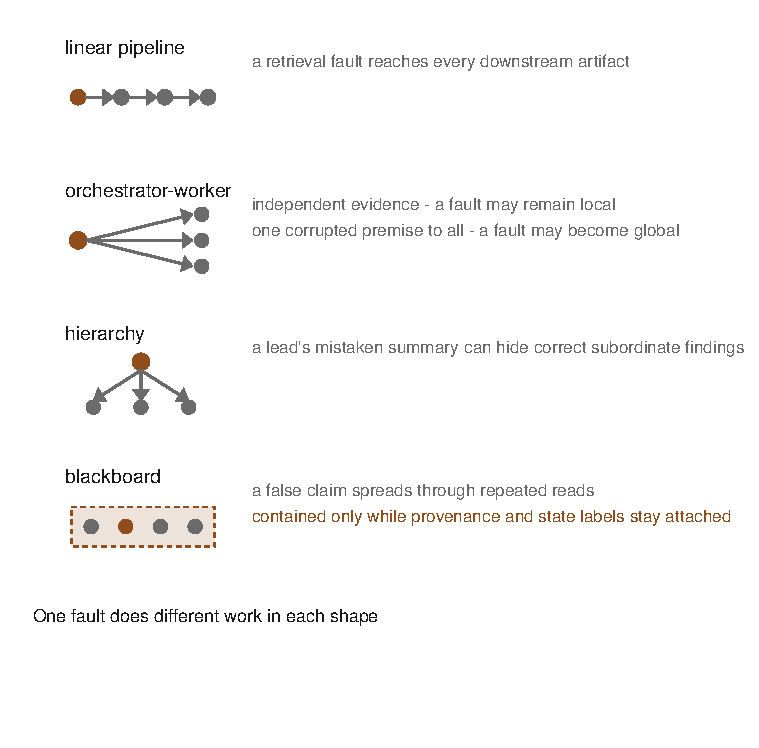
\includegraphics[keepaspectratio,alt={Fault propagation depends on collaboration topology, ranging from downstream contamination in pipelines to contained local errors when shared systems preserve provenance and state labels.}]{figures/ch17-topology-faults.pdf}}
\caption{Fault propagation depends on collaboration topology, ranging from downstream contamination in pipelines to contained local errors when shared systems preserve provenance and state labels.}
\end{figure}

Containment is conditional. A shared corrupted premise, an inaccurate lead summary, or repeated reads of an unqualified claim can turn a local error into a global one.

\Needspace{5\baselineskip}

Observation routes are therefore part of correctness. Record:

\begin{itemize}
\tightlist
\item
  which workers see raw tool output;
\item
  which receive only summaries;
\item
  whether a downstream component can request new upstream evidence;
\item
  whether workers see others' tentative conclusions before forming their own;
\item
  where contradictory results converge; and
\item
  which component can mark shared state disputed or invalid.
\end{itemize}

These properties govern error correlation, recovery, and attribution even when every worker uses the same model and prompt.

Runtime oversight can represent the topology as an interaction graph whose nodes are workers and artifacts and whose edges are messages or state transitions. That representation is a thinly supported companion idea and has not been validated as a monitoring standard. It remains a useful inspection tool because it exposes unreachable reviewers, unexpected broadcasts, and missing convergence paths.

Topology should be tested through faults, not inferred from diagrams.

\Needspace{5\baselineskip}

For a pipeline:

\begin{itemize}
\tightlist
\item
  remove or corrupt one stage output;
\item
  verify that downstream work stops or marks the state incomplete;
\item
  test whether the pipeline can widen or restart upstream.
\end{itemize}

\Needspace{5\baselineskip}

For an orchestrator-worker system:

\begin{itemize}
\tightlist
\item
  delay one worker;
\item
  inject contradictory findings;
\item
  corrupt one worker's input;
\item
  verify that the orchestrator distinguishes missing, late, and conflicting evidence.
\end{itemize}

\Needspace{5\baselineskip}

For a hierarchy:

\begin{itemize}
\tightlist
\item
  insert a critical minority finding at a subordinate level;
\item
  verify that it survives summarization;
\item
  test whether the lead can request source evidence.
\end{itemize}

\Needspace{5\baselineskip}

For a blackboard:

\begin{itemize}
\tightlist
\item
  submit conflicting updates;
\item
  verify that provenance and ordering remain attached;
\item
  preserve unresolved status rather than allowing last-write-wins to manufacture agreement.
\end{itemize}

The strongest evidence here, from Jia et al., concerns synthetic injected faults. Naturally occurring production faults lie outside that result, and the injected fault distribution determines what the comparison can show.

The reported closed-loop advantage supplies a reason to run local fault tests. It does not remove their necessity.

\Needspace{5\baselineskip}

The acceptable topology is the simplest one that:

\begin{itemize}
\tightlist
\item
  preserves the evidence the task requires;
\item
  contains representative faults;
\item
  exposes incomplete and disputed state;
\item
  keeps aggregation failures observable; and
\item
  clears the live single-agent gate on the target workload.
\end{itemize}

\section{Dispatch only work whose dependencies are satisfied}\label{dispatch-only-work-whose-dependencies-are-satisfied}

In a narrative reconstruction from my workflow harness, six planned work items initially appeared ready to run together. A pre-dispatch overlap check showed that four touched the same adapter file and its test. The schedule therefore became two waves. Three items could run in parallel, including two disjoint changes and one low-risk item from the colliding group. The remaining three ran sequentially in increasing risk order.

The scheduler selected a maximum independent set of nonconflicting work. Maximizing the number of simultaneous workers was not the objective.

The work-item identities, overlap matrix, and dispatch log from that sweep were not preserved, so the example illustrates the scheduling decision without providing an auditable result. The evidence for dynamic task graphs is also directional. The example cannot strengthen it.

A \textbf{dependency graph} represents units of work as nodes and prerequisites or conflicts as edges. It becomes a \textbf{task graph} when the runtime uses those records to decide which nodes are eligible for dispatch. A node becomes ready only when its prerequisites have completed successfully and its declared resources do not conflict with another running node. Independent work need not wait behind an unrelated serial step.

Execution can also change which work exists. A repository investigation may begin with one node that locates the affected adapter, then create package-specific repair nodes only after the adapter is identified. A failed compatibility check may add a migration node and block integration. A fixed schedule must either predict those branches in advance or leave workers idle while a central planner reconstructs dependencies from messages.

Dynamic dispatch does not mean unconstrained autonomy. The runtime performs a mechanical transition from \texttt{blocked} to \texttt{ready} when explicit conditions become true. Semantic decisions, such as whether a test failure warrants a new task, still require a model or person to propose the node and its dependencies. The scheduler validates that record and executes it under policy.

Yu et al.~(\href{https://arxiv.org/abs/2503.07675}{2025}) provide the only direct systems report attached to this practice, at directional strength. DynTaskMAS contains no controlled comparison between dynamic and fixed scheduling. The study compared parallel with serial execution on one seven-agent travel-planning workload. It did not compare a dynamic schedule with a fixed parallel schedule or isolate the task graph from the asynchronous execution engine.

The reported improvement therefore shows only that parallel execution outperformed serial execution in that setting. It does not show that dynamic scheduling outperformed a well-designed fixed schedule.

Rose et al.~(\href{https://arxiv.org/abs/2605.15132}{2026}) in APWA, Luo et al.~(\href{https://arxiv.org/abs/2502.13965}{2025}) in Autellix, and Masters et al.~(\href{https://arxiv.org/abs/2510.02557}{2025}) in the Manager Agent research challenge provide separate directional examples of related planning and scheduling architectures. None replicates a dynamic-versus-fixed comparison.

No controlled result in the cited evidence establishes that a dynamic dependency graph improves repository work relative to a fixed schedule.

The narrower systems argument applies when dependencies vary during execution. If independent branches exist, their prerequisites are observable, and their durations are uncertain, an explicit graph can expose safe concurrency without forcing unrelated work through one serial queue. If the workflow is short, fixed, and inexpensive, a graph scheduler may add persistence and recovery complexity without creating useful parallelism.

Dependency accuracy is the central risk. A missing edge can dispatch two workers that edit the same file, migrate the same schema, or invalidate each other's assumptions. A false edge serializes work that could safely overlap.

\Needspace{5\baselineskip}

File overlap is only one conflict signal. Work may also conflict through:

\begin{itemize}
\tightlist
\item
  generated artifacts;
\item
  shared test fixtures;
\item
  database schemas;
\item
  deployment environments;
\item
  locks or leases;
\item
  external services;
\item
  mutable caches; or
\item
  logical invariants spanning disjoint files.
\end{itemize}

Each node therefore needs enough state to support both scheduling and recovery:

\begin{verbatim}
node_id: stable logical identity
inputs: immutable artifact versions
depends_on: prerequisite nodes that must succeed
conflicts_with: resources or nodes that cannot overlap
owner: currently assigned worker
attempt: retry identity
status: blocked | ready | running | succeeded | failed
outputs: versioned artifacts and supporting evidence
\end{verbatim}

The attempt identity prevents a late response from an expired worker from overwriting a successful retry. Immutable input versions reveal when a ready node was planned against stale state. Versioned outputs allow downstream nodes to distinguish attempts that produced different artifacts.

These requirements come from the execution topology. Drawing the graph supplies none of them.

In my workflow harness, notification-driven dispatch ends the coordinating turn after work is assigned and resumes it when completion events arrive. This avoids a polling loop that consumes attention while no state has changed. Mechanical parallel-set detection checks dependency layers, blocking edges, and overlapping file paths.

Those rules illustrate the mechanism. They do not provide comparative performance evidence.

A per-step time limit contains a slow or failed worker only when expiration produces and propagates a real failure. Treating a timeout as success destroys the evidence of failure and may release downstream nodes without their required inputs. The schedule then appears healthy because it erased the event needed to diagnose it.

Dispatch should fail closed:

\begin{verbatim}
worker exceeds time limit
    -> attempt fails visibly
    -> dependent nodes remain blocked
    -> retry, escalation, or cancellation policy runs
\end{verbatim}

Retries require the same discipline. A retry creates a new attempt for the same logical node rather than a second independent task. The scheduler must either establish that repeated execution is idempotent or isolate side effects before trying again. Otherwise a timeout can produce duplicate comments, partial writes, or two workers claiming the same resource.

\Needspace{5\baselineskip}

Dynamic graphs are most useful when they expose decisions that were previously implicit. The runtime should be able to explain:

\begin{itemize}
\tightlist
\item
  why a node remains blocked;
\item
  which successful output released it;
\item
  which conflict prevents concurrent execution;
\item
  which attempt currently owns it;
\item
  which input version it was planned against; and
\item
  why a failure created, removed, or blocked another node.
\end{itemize}

If those answers cannot be reconstructed, the graph has become another hidden coordinator rather than an observable allocation mechanism.

\section{Promote topology from a recorded comparison}\label{promote-topology-from-a-recorded-comparison}

A structural redesign should end in a reproducible allocation decision. A diagram and a promising demonstration are not enough. The following protocol is narrow enough to apply to an existing workflow while preserving the distinctions developed in this chapter.

\section{1. Select one persistent failure class}\label{select-one-persistent-failure-class}

Use repeated paired runs across the current and upgraded model configurations. Preserve the first-upstream-failure assignment from Chapter 10.

Do not begin from a broad objective such as ``improve collaboration.'' Name the failure class whose path the structural change is expected to interrupt.

\section{2. Draw the current causal path}\label{draw-the-current-causal-path}

\Needspace{5\baselineskip}

Mark:

\begin{itemize}
\tightlist
\item
  where evidence originates;
\item
  where interpretation occurs;
\item
  where state becomes durable;
\item
  where authority changes hands;
\item
  where verification occurs; and
\item
  where the final decision converges.
\end{itemize}

Identify the smallest boundary at which the target failure could have become observable and stoppable.

\section{3. Preserve the live single-agent baseline}\label{preserve-the-live-single-agent-baseline}

\Needspace{5\baselineskip}

Replay the existing single-agent workflow on the current golden set. Record:

\begin{itemize}
\tightlist
\item
  pass\textsuperscript{k} or the selected reliability measure;
\item
  the chosen cost axis;
\item
  elapsed time;
\item
  tool and model use;
\item
  failures by class; and
\item
  the complete configuration identity.
\end{itemize}

Keep this baseline executable for later model releases. A topology should not receive permanent credit from a comparison against an obsolete single-agent system.

\section{4. Specify one structural treatment}\label{specify-one-structural-treatment}

\Needspace{5\baselineskip}

The treatment may be:

\begin{itemize}
\tightlist
\item
  a deterministic verification loop;
\item
  a specialized role;
\item
  a structured handoff;
\item
  a different communication topology;
\item
  a new aggregation rule; or
\item
  a dependency-aware dispatcher.
\end{itemize}

State which boundary changes and which causal path the change is expected to interrupt. Avoid combining several architectural changes unless the experiment is explicitly evaluating the combined system.

\section{5. Record the promotion rule before execution}\label{record-the-promotion-rule-before-execution}

\Needspace{5\baselineskip}

The rule should include:

\begin{itemize}
\tightlist
\item
  a task-success floor;
\item
  a reliability requirement;
\item
  a cost ceiling;
\item
  a latency limit where relevant;
\item
  a mechanism condition; and
\item
  any required fault-containment result.
\end{itemize}

A mechanism condition might require at least one delegated result to be consumed by the aggregator or require the scheduler to dispatch at least one pair of independent nodes concurrently. When candidates are voted on or synthesized, add a check for whether an oracle-correct candidate was retained or discarded.

\section{6. Inject a representative fault}\label{inject-a-representative-fault}

\Needspace{5\baselineskip}

Choose a fault matched to the proposed structure:

\begin{itemize}
\tightlist
\item
  For a pipeline, corrupt or omit an upstream artifact.
\item
  For an orchestrator, delay one worker or return contradictory findings.
\item
  For a hierarchy, place a critical result in a minority branch.
\item
  For a blackboard, submit conflicting updates and inspect ordering and provenance.
\item
  For a task graph, omit a dependency, introduce a false conflict, expire a worker attempt, or return a late completion.
\end{itemize}

Verify that incomplete or disputed state remains visible and that downstream work does not proceed as though the missing evidence existed.

\section{7. Run paired repeated trials}\label{run-paired-repeated-trials}

Run baseline and treatment on the same task versions. Keep the model, harness, permissions, evaluator, and execution environment fixed except for the declared structural change.

\Needspace{5\baselineskip}

Report separately:

\begin{itemize}
\tightlist
\item
  correctness;
\item
  reliability;
\item
  latency;
\item
  total computation;
\item
  monetary or token cost;
\item
  coordination failures;
\item
  usability or review burden; and
\item
  target failure-class frequency.
\end{itemize}

Inspect traces to confirm that delegation, scheduling, coordination, and aggregation actually occurred. A configured mechanism that never enters the execution path has not been evaluated.

\section{8. Promote, retain, or redesign}\label{promote-retain-or-redesign}

Promote only when the treatment clears the recorded success, reliability, cost, mechanism, and fault-containment conditions.

Retain the baseline when additional structure does not earn its coordination cost.

Redesign when the trace shows that the treatment changed a boundary but left the target failure path intact. The next experiment may require a narrower specialist role, another handoff field, a different aggregation rule, a corrected dependency model, or no additional worker.

The resulting record should be understandable without trusting the architecture's name. Promotion depends on whether the observed execution supports the claimed benefit, not on whether the design can be described as dynamic, hierarchical, multi-agent, or dependency-aware.

\section*{Sources and evidence}

The evidence grouping on each entry below comes from its catalog record. Author-system cases in this chapter are narrative illustration and are not part of the evidence base.

\begin{itemize}
\tightlist
\item
  Bertalani\v{c}, et al.~2026. \emph{The Cost of Consensus}. arXiv:2605.00914. Exploratory evidence on aggregation failure; Chapter 5 carries the reported oracle-gap result.
\item
  Böckeler, Birgitta. 2026. ``Harness Engineering.'' MartinFowler.com, February 17. Practitioner account based partly on vendor-reported Codex-team practice.
\item
  Cemri, M., et al.~2025. ``Why Do Multi-Agent LLM Systems Fail?'' arXiv:2503.13657. MAST failure taxonomy and benchmark-framework interventions.
\item
  Chun, Jina, et al.~2025. ``Is Multi-Agent Debate the Silver Bullet?'' arXiv:2503.12029. Audit-retained strong evidence on debate performance against task baselines; reports inference cost across debate variants and leaves the single-model cost comparison open.
\item
  Huang, Jia, and Joey Tianyi Zhou. 2026. ``A Two-Dimensional Framework for AI Agent Design Patterns: Cognitive Function and Execution Topology.'' arXiv:2605.13850. Directional taxonomy of topology choices.
\item
  Jia, J., et al.~2026. ``MAS-FIRE: Fault Injection and Reliability Evaluation for LLM-Based Multi-Agent Systems.'' arXiv:2602.19843. Synthetic fault injection across three architectures.
\item
  Jain, Prateek. 2026. ``Harness Engineering: The New DevOps Layer for AI Agents.'' r/devops, May 27. Anecdotal practitioner account.
\item
  Kim, T., et al.~2026. ``Why Do AI Agents Systematically Fail at Cloud Root Cause Analysis?'' arXiv:2602.09937. OpenRCA evidence on failure persistence across capability tiers and protocol intervention.
\item
  Kumar, et al.~2026. \emph{AgentForge}. arXiv:2604.13120. Directional evidence on multi-agent design.
\item
  Li, et al.~2026. \emph{SIMAS}. arXiv:2606.00655. Audit-retained strong evidence on token cost, non-monotonic scaling, and debate versus self-correction.
\item
  Luo, et al.~2025. \emph{Autellix}. arXiv:2502.13965. Directional scheduling and orchestration example.
\item
  Masters, et al.~2025. \emph{Manager Agent research challenge}. arXiv:2510.02557. Directional planning and scheduling example.
\item
  Qian, et al.~2024. \emph{MacNet}. arXiv:2406.07155. Directional evidence on network scaling.
\item
  Rose, Evan, et al.~2026. \emph{APWA: A Distributed Architecture for Parallelizable Agentic Workflows}. arXiv:2605.15132. Directional orchestration example.
\item
  Shang, Wenlong. 2026. \emph{``Theater of Mind'' for LLMs: A Cognitive Architecture Based on Global Workspace Theory}. arXiv:2604.08206. Directional blackboard and global-workspace design; single-author architecture proposal, not a controlled measurement.
\item
  Tian, et al.~2025. ``Beyond the Strongest LLM.'' arXiv:2509.23537. Directional evidence on multi-agent teams.
\item
  Yu, Junwei, Yepeng Ding, and Hiroyuki Sato. 2025. \emph{DynTaskMAS}. arXiv:2503.07675. Directional parallel-versus-serial result on a seven-agent travel-planning workload; no controlled dynamic-versus-fixed comparison.
\item
  Zhao, et al.~2026. \emph{ATOM}. arXiv:2605.26178. Audit-retained strong evidence on difficulty-conditioned topology across six short-form benchmarks.
\end{itemize}

\textbf{Author-system illustration cited inline}

\begin{itemize}
\tightlist
\item
  Not an evidence item: CodeProbe, the author's task-mining evaluation tool, \href{https://github.com/sjarmak/codeprobe}{public repository}. Named inline for the preamble rerun described in the opening, which is narrative illustration.
\end{itemize}


\chapter{Cost-aware fleet scheduling and model routing}\label{cost-aware-fleet-scheduling-and-model-routing}

A fleet can raise throughput while raising the cost of each accepted result, and only the fleet's own traces can establish whether it did. Concurrent execution, together with the willingness to take on work a human team would have left queued, exposes more work to model inference, review, and recovery. Throughput alone therefore does not establish the economic result.

The evidence for changing that outcome is thin, and most of it is transferred from other fields. This chapter has one strong software-engineering result about cheap baselines, directional literature from observatory and compute-cluster scheduling, and my own fleet replay, which is narrative illustration with no independent evidentiary weight. The relevant evidence cluster has one strong item rather than zero.

Astronomical observation scheduling is the dominant transfer domain, in two forms: a survey telescope's nightly planner, and a gravitational-wave follow-up scheduler built on the same facility. Learned compute-cluster scheduling is the second domain and search-based software engineering the third. Budget-constrained bandit theory and router calibration cover the routing decision alone rather than a complete fleet.

These are schedulers for telescopes and compute clusters. None of the cited works claims results for software agent fleets. The decision architecture transfers: re-decide from current state, cap the time spent deciding, compare against cheap alternatives, and preserve enough measurement to detect a bad policy. Cadence, threshold, cost ratio, and performance constants do not transfer with it.

Allocation policy is easy to mistake for a local configuration choice. In an agent fleet, the policy determines which model receives a request, which queued item moves first, whether running work remains fixed, and when the system discards an obsolete plan. These choices couple inference cost to elapsed time, reviewer load, and the probability that completed work will survive evaluation. A repair loop can consume the savings from a cheaper call. A schedule that is better on paper is not better in operation if computing it delays the work past its deadline. I therefore treat scheduling and routing as decisions under measurement.

\section{Name the decision before reaching for the algorithm}\label{name-the-decision-before-reaching-for-the-algorithm}

Cheapest-sufficient routing means choosing, for each task, the least expensive worker predicted to meet that task's declared requirement. The worker may be a model tier, a model-plus-tool configuration, or another execution pool with a known price. The important word is sufficient. The router is not minimizing the invoice in isolation, and it is not assigning every task class to a model through a hand-written rule. It estimates expected performance and expected cost for the request in front of it, then chooses the lowest-cost option that satisfies the stated tradeoff. This definition leaves open how performance is predicted and how sufficiency is expressed. These are deployment decisions with consequences for calibration and evaluation.

Shipping the incumbent at the deadline means placing a hard time cap on schedule computation and executing the best feasible plan available when the cap expires. A feasible plan respects the constraints that cannot be violated, such as capacity, deadlines treated as hard, and work already in flight. The incumbent is the best such plan found so far. Waiting longer may find a better plan or prove that the current one is optimal, but the schedule has operational value only while it describes a world that still exists. With a cap, decision latency is chosen rather than discovered.

The optimality gap records how far the shipped solution might be from the best possible one, using the best bound known when the cap was reached. The gap retains information about the remaining uncertainty in solution quality. Shipping an incumbent without its gap records two different states as one: a plan known to be nearly best, and a merely feasible plan found before the search made much progress. Operations may reasonably execute both. Evaluation should not treat them as equivalent.

\begin{figure}
\centering
\pandocbounded{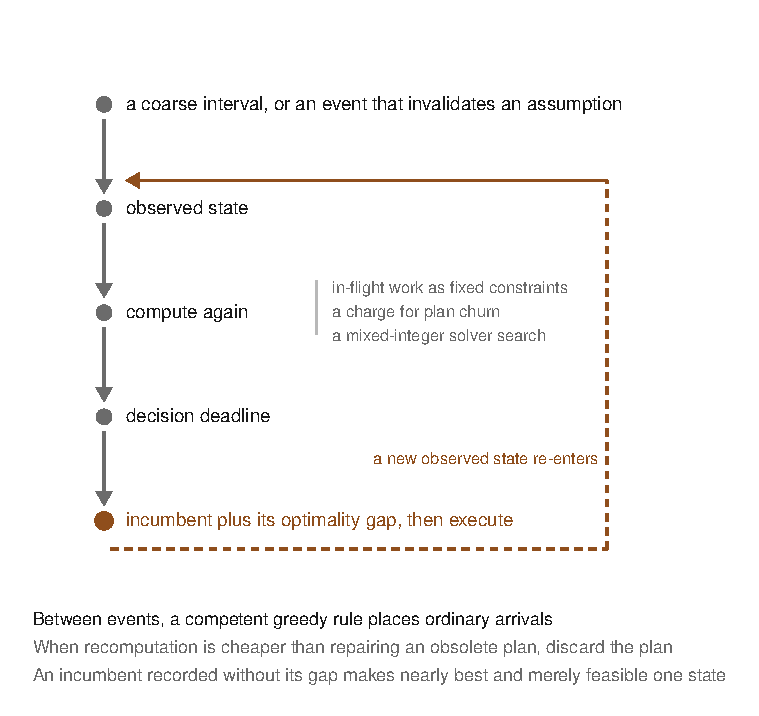
\includegraphics[keepaspectratio,alt={The re-decision loop recomputes from observed events under fixed work and churn costs, then executes a deadline capped incumbent while retaining its optimality gap.}]{figures/ch18-redecision-loop.pdf}}
\caption{The re-decision loop recomputes from observed events under fixed work and churn costs, then executes a deadline capped incumbent while retaining its optimality gap.}
\end{figure}

Ordinary arrivals remain greedy between events, and the plan is discarded only when fresh optimization costs less than repairing obsolete work.

These terms specify decisions. A fleet operator needs to decide what counts as sufficient, how long schedule computation may run, which constraints are inviolable, and what quality information must survive execution. The companion catalog contains the algorithmic patterns. The narrower question here is whether these decisions produce lower cost or more reliable flow on the fleet's own workload.

\section{Re-decide cheaply and ship the incumbent}\label{re-decide-cheaply-and-ship-the-incumbent}

An observatory scheduler can spend the night improving a plan that clouds have already invalidated, or it can compute another imperfect plan from the sky it can still observe. Bellm et al.~(\href{https://arxiv.org/abs/1905.02209}{2019}) described the Zwicky Transient Facility taking the second approach, in production since 2018. It re-solves its nightly integer program when conditions invalidate the schedule instead of enumerating weather scenarios in advance. The support for transferring this choice to agent fleets is three directional literature items from observatory scheduling, with no strong result and no software-fleet measurement among them. The recommendation is therefore limited to choosing and measuring a re-decision policy. The cadence remains an agent-fleet deployment decision.

The schedule should be treated as the current output of a control loop. At a coarse interval, or after an event that invalidates an important assumption, the scheduler computes again from observed state. Between those events, a competent greedy rule can place ordinary arrivals without paying the cost of a full solve. If recomputation is cheaper than repairing an obsolete plan, the obsolete plan should be discarded. The comparison must include decision latency. An excellent schedule delivered after the queue has changed is a schedule for a fleet that no longer exists.

Current state includes more than the queue. Running work consumes capacity, may hold a repository lease or a review slot, and may have produced state that another worker cannot cheaply reconstruct. A re-solve should represent that in-flight work as fixed constraints unless preemption has been separately justified. It should also charge for plan churn, meaning avoidable reassignment or resequencing that makes workers discard useful preparation. The companion-catalog pattern \texttt{design-the-online-rescheduling-loop} treats cadence, invalidation triggers, and this churn penalty as parts of the scheduling algorithm. They are not operational details to add after selecting an objective.

At the decision deadline, execute the mixed-integer solver's incumbent and record its optimality gap. This prescription follows from the mismatch between proof time and operational time. Solvers often find a feasible plan before they finish establishing how close it is to the best plan, while new arrivals and changing capacity continue to age the state on which that plan was built. The cap prevents schedule computation from becoming another queue. The stored gap makes later analysis possible. Operators can then ask whether large gaps coincide with worse flow, whether more solve time would have changed executed choices, and whether a simpler rule performs just as well.

Parazin et al.~(\href{https://arxiv.org/abs/2203.00013}{2022}) measured a mixed-integer scheduler for gravitational-wave follow-up against a tuned greedy heuristic, and neither method won outright. At a 500-second cap, their scheduler and the gwemopt heuristic each did better on different skymaps, and only 37 of 97 well-localized skymaps improved under the optimization comparison the paper reported. Across 951 simulated events, the headline result favored a hybrid of the two by roughly 3 to 11 percent in detection efficiency. A 100-second cap, they reported, would have truncated only 64 more schedules without substantial efficiency loss.

These figures are directional evidence from a gravitational-wave follow-up workload rather than fleet parameters. They support measuring the cap, the gap, and a hybrid, each against a tuned simple rule. They also argue against assuming in advance that either the optimizer or the simple rule will win.

Naghib et al.~(\href{https://arxiv.org/abs/1810.04815}{2019}) described a second observatory design that makes the same point about state: a feature-based, memoryless policy that decides again at every step from current state. `Memoryless' here does not mean that the system forgets durable facts. It means that the next scheduling choice does not depend on preserving a brittle sequence of earlier planned choices. Interruptions are absorbed when the scheduler observes the new state and makes another decision. Their evidence comes from a framework and a simulation. It therefore establishes a plausible architecture rather than a measured benefit for agent execution.

The global problem and the local problem should remain distinct. A fleet-wide allocator decides how scarce model tiers, reviewers, or execution pools are divided across work. A per-worker dispatcher decides which eligible item a particular worker takes next. The companion catalog records this as \texttt{split-fleet-scheduling-into-global-and-local-levels}. Combining both decisions in one opaque score makes it difficult to determine whether a bad outcome came from resource allocation or queue order. It can also cause local dispatch to undo a capacity decision that the global layer just made.

There is a more ambitious companion pattern, \texttt{formalize-work-as-constraints-and-solve-globally}, whose cataloged lineage reaches Hubble scheduling in 1990. It proposes expressing work requests in one constraint language so the allocator can solve across them. This architecture is useful only if the request representation captures the constraints that operations actually enforce. A nominally global solution built from incomplete deadlines, missing affinity constraints, or false independence assumptions can be less coherent than separate local rules. \texttt{audit-the-allocation-layer} is therefore marked as an aside in the catalog: name the execution, planning, and optimization levels, then inspect which policy actually dispatches work. Its observatory analogy has no software-side measurement.

Probe costs belong in the same accounting. The thin-support aside \texttt{probe-only-above-an-uncertainty-threshold} asks whether a dry run, canary, or classifier call can reduce enough uncertainty to repay its cost. Its theory comes from adversarial single-machine scheduling. Its constant therefore does not transfer. The usable question is local: for which uncertain requests does a probe change the chosen worker or the schedule often enough to justify the extra latency and inference? If that answer cannot be recovered from logs, probing is another unmeasured policy.

This decision has an explicit boundary. The survey behind the cited corpus does not see the major USENIX and ACM cluster-scheduling literature. Agent runtime variance is also partly endogenous. Repeated tool failure, unstable environments, and unnecessary retries should be repaired at their source before the scheduler is asked to absorb them. Nor does any cited source establish a general rule against preempting long agent sessions. Fixing running work during a re-solve is a conservative representation of current commitments rather than evidence that preemption is always wrong.

The cadence and cap should be set through a short pilot, with the incumbent and its gap retained at every decision and the resulting trace compared against a tuned greedy policy. The companion entry \texttt{pilot-to-pick-the-algorithm-then-commit-the-budget} states the same budget logic. Spend a small amount discriminating among methods, then commit the operating budget to the one that performed better. The design decision is defensible when the trigger, cap, churn charge, and treatment of in-flight work are explicit. Its value remains an empirical question until the fleet's own traces answer it.

\section{Route each request to the cheapest sufficient model}\label{route-each-request-to-the-cheapest-sufficient-model}

Support for cheapest-sufficient routing is three directional literature items and zero strong results. Cayci, Eryilmaz and Srikant (\href{https://arxiv.org/abs/2003.00365}{2020}) developed budget-constrained online learning under broad cost and reward distributions. Somerstep et al.~(\href{https://arxiv.org/abs/2502.03261}{2025}) analyzed a calibrated static router. Li (\href{https://arxiv.org/abs/2502.02743}{2025}) reported preference-conditioned dynamic routing in a single-author preprint. All three evaluated formulations or benchmarks, and none evaluated a production software-agent fleet. This entry therefore defines a routing decision and the measurements needed to test it, and it does not establish that a learned router will reduce the cost of a particular fleet.

My agent-fleet orchestrator illustrates the starting condition. Its dispatch policy is a static string in each agent configuration. Every execution pool is assigned a model in advance, and there is no per-request performance estimate, cost model, lookahead, or deadline field. The static table is legible and predictable, and it provides the fallback when a more selective router has too little evidence. It does, however, make request difficulty invisible to dispatch.

A cheapest-sufficient router replaces the static per-model assignment with two estimates for every available model on the current request: expected performance and expected cost. It then selects the least expensive candidate predicted to satisfy the declared requirement. Somerstep et al.~(2025) analyzed this plug-in structure in CARROT and argued that its routing overhead is negligible, because a routing decision requires only evaluating those two predictors for each candidate model. That structure depends on calibration, meaning that predicted performance must correspond to observed performance on the deployment distribution. A mathematically clean selection rule cannot recover from a predictor that assigns unwarranted confidence to unfamiliar work.

The requirement must also be operational rather than rhetorical. `Good enough' might mean passing an executable check, staying below a defect probability, meeting a review rubric, or satisfying a cost-quality tradeoff selected by the caller. Each choice defines a different routing target. The roughly 15-fold token premium for some fan-out topologies discussed in Chapter 17 gives that choice real economic weight, but token count alone is not the objective. A cheap model that triggers repeated repair and review may produce a higher accepted-result cost than the expensive model it displaced.

When outcome feedback accumulates, the router can be updated as a budget-constrained bandit, for example by Thompson sampling, with the algorithmic treatment left to the companion catalog. Cayci, Eryilmaz and Srikant (2020) established an asymptotic regret guarantee under stated moment conditions that permit heavy-tailed, correlated, and even negative cost-reward pairs. These properties resemble agent dispatch more closely than a world of bounded, independent rewards. The guarantee still does not tell an operator whether a code review score represents useful work, and it says little about behavior during the finite, early period in which production exploration is most costly.

Online updating addresses a real problem in static routing, because both models and workloads change. A model revision can alter which tier is sufficient, and a new repository or task mix can move the request distribution outside the router's calibration data. Li (2025) conditioned routing on a user-selected performance and cost preference, allowing one learned policy to express a family of tradeoffs at inference time. The reported support is benchmark evidence from a single-author preprint. It supports testing preference conditioning, but calibration under delayed code outcomes remains untested.

The reward definition is the controlling measurement choice. For code tasks, the observable signals arrive at different times and answer different questions. A test result may be immediate but incomplete. Review can catch a defect later. Rework, rollback, or user rejection can occur after the router has already treated the request as a success. Combining these into one reward is a construct-validity decision outside the routing mathematics, and it should be versioned so that a policy trained under one definition is not silently compared with a policy trained under another.

A learned policy should stay advisory until its recommendations correlate with an outcome measured outside the router and relevant to accepted work. In advisory mode, the system records the requested route, the route actually taken, estimated cost and performance, uncertainty, and the eventual outcome, without granting the policy control. The thin-support companion aside \texttt{log-scheduling-decisions-for-selection-effect-modeling} adds a necessary field: record why a request was routed. Without that reason, later analysis cannot distinguish a model's performance from the selection process that sent it easier or harder work.

When observations are sparse, the system should fall back to the static cost-performance table. That floor is exactly today's configuration, and its behavior can be measured directly. The router should take control only when the evidence is dense enough to estimate its errors. A rare task family, a new model, or a reward version with few completed outcomes should stay on the floor until the router exposes its uncertainty.

Calibration data can fail before deployment begins. Benchmark-derived routing sets may encode artifacts of the benchmark into the predictor, including prompt regularities, scoring conventions, and an unrealistically fixed menu of models. CARROT's formulation assumes a static model pool. Production pools are not static: prices change, versions are retired, rate limits vary, and tool compatibility can remove a model from consideration. Each change either requires recalibration or creates a region in which the policy is extrapolating.

Online exploration imposes a further cost. The policy must sometimes choose an option of uncertain value to learn anything, and the request routed under that choice is real production work. Budget constraints make the cost visible but do not decide who may bear it. Operators need an exploration budget, exclusion rules for high-consequence work, and a stop condition tied to observed error. Guarantees that become useful only after many decisions do not excuse poor behavior during the learning period.

The companion pattern \texttt{cost-cascade-routing} covers a different response to uncertainty: begin with a cheaper route and escalate when calibrated confidence is insufficient. In that pattern's supporting evidence, Chang (\href{https://arxiv.org/abs/2604.12262}{2026}) reported that confidence-gated cascade routing often beat always-on strong-model fan-out on both cost and quality. This result supports only the catalog pointer. A cascade also changes latency and couples the stages through the escalation signal. It must therefore be compared as a complete route, with cost measured across all calls.

The decision record for a router should include the sufficiency requirement, reward version, calibration population, model-pool version, uncertainty, exploration budget, and static fallback. The evaluation should report accepted-result cost and failures by request class, not only average token spend. Cheapest-sufficient routing is useful as a testable economic policy because it states what is being predicted and what tradeoff is being chosen. It cannot repair an unrepresentative calibration set or a reward that measures the wrong outcome.

\section{Replay fixed arrival traces before changing policy}\label{replay-fixed-arrival-traces-before-changing-policy}

In my own agent fleet, the interesting scheduling idea lost to a one-word configuration change. I replayed eleven weeks of traffic and found that a four-feature weighted index performed within 0.1 percent of plain priority banding. This result has narrative weight only, and it is not load-bearing evidence for the recommendation. The strong support in this entry comes from SWAY, the controlled software-engineering result of Chen et al.~(\href{https://arxiv.org/abs/1608.07617}{2016}), which shows why a proposed search method must beat a cheap baseline. Decima, from Mao et al.~(\href{https://arxiv.org/abs/1810.01963}{2018}), and the telescope-network work of Lampoudi, Saunders and Eastman (\href{https://arxiv.org/abs/1503.07170}{2015}) provide directional support for learned scheduling and known-optimum validation. Fixed-arrival replay itself remains a reasoned transfer rather than a directly controlled fleet result.

An arrival trace is a time-ordered record of work entering the system, including the information available when each item arrived. A dispatch policy is the rule that decides which eligible item receives a resource next. First-come scheduling orders eligible work by arrival time, subject only to constraints that make an item impossible to run. A replay harness is a read-only re-execution of recorded arrivals under a candidate dispatch policy. It differs from the single-run trace replay used for debugging in Chapter 9, because this harness holds a workload sequence fixed while replacing the policy that acts on it.

The ledger needs, at minimum, arrival times, priorities, claims, durations, outcomes, and review verdicts. It also needs the resource state that constrained each decision, or a defensible reconstruction of that state. If the historical record omits capacity, cancellations, model eligibility, or work already running, the replay may create choices that were never available. Missing decision context is not neutral noise. It changes the feasible schedule.

Holding arrivals fixed turns the comparison into a paired design. Every candidate encounters the same demand in the same order. A difference in simulated flow is therefore attributable to the policy and its interaction with recorded state, rather than to a busier Tuesday in one run. This does not make the simulation causal in every respect. It removes one large source of variation that routinely overwhelms scheduler comparisons.

The first run should be a validation run, not a policy contest. Construct small cases whose best schedule is known, including simultaneous arrivals, a resource that becomes unavailable, a priority inversion, and work that cannot run in the same execution pool. Confirm that the replay clock, eligibility checks, claim duration, and completion events reproduce the known answer. Lampoudi, Saunders and Eastman (2015) derived an integer-program formulation for the Las Cumbres telescope network and reported computational results verifying it at realistic problem sizes. The transferable practice is to test a scheduling kernel on instances with known optima before trusting its output on a historical trace.

The second run establishes cheap baselines. Compare first-come scheduling, a simple priority sort, and random oversampling with the proposed policy. Random oversampling generates several cheap randomized schedules and retains the best according to the declared objective. Chen et al.~(2016) built SWAY by sampling a very large candidate population down to better solutions rather than evolving repeated generations. Across several software-engineering models it was competitive with state-of-the-art evolutionary algorithms at far lower compute cost, and they proposed it explicitly as a baseline for search-based software engineering. The controlled result supports the discipline. An elaborate optimizer that cannot beat a cheap alternative has not earned adoption.

The baseline objective must be written before inspecting the candidate results. Mean completion time, priority-weighted flow time, deadline misses, accepted-result cost, and reviewer delay describe different failures. A lower overall mean can coexist with severe delay for one priority or work class. Starvation is persistent denial or extreme delay to a class because other eligible work repeatedly moves ahead of it. Report latency and failure by class, and define a guard that would reveal starvation even when the fleet-wide average improves.

My fleet's work ledger contained 1,286 work items across 22 execution pools in the eleven-week replay. Age-only first-come scheduling produced 6.84 hours of priority-weighted flow time. A hybrid rule, a plain priority rule, and my four-feature weighted index each produced 6.70 hours, within 0.1 percent of one another. P1 tail latency moved from 20.4 hours to 18.8 hours without a starvation-guard trip.

I had recorded a 15 percent acceptance threshold before the replay ran. The weighted index therefore failed its gate. The four-feature index was the interesting idea, and the replay is the reason it did not ship. These numbers explain what the protocol prevented me from building. They do not establish an expected effect for another fleet.

The distribution of capacity explained more than the aggregate did. The visible gain concentrated in one contended pool, meaning an execution pool in which eligible work regularly exceeded available capacity. An uncontended execution pool, in which capacity usually met demand, showed nearly no change across policies. This is the expected shape of a real scheduling effect. A proposed policy that claims large gains when work rarely waits for a resource should be treated with suspicion, because queue order then has little opportunity to change anything.

Decima provides a useful but bounded comparison. It learned cluster scheduling under continuous stochastic arrivals and was evaluated on a 25-node Spark cluster. Mao et al.~(2018) reported at least a 21 percent average job-completion-time improvement over hand-tuned heuristics, and improvements up to twofold at high load. These measurements support learned scheduling in that cluster workload. They do not test fixed-arrival replay, and they do not transfer a performance expectation to agent work. The relevant transfer is experimental. Preserve the arrival process when comparing policies, then look for effects in the places where resources are actually contested.

Historical replay also preserves historical selection. Work absent from the ledger remains absent, including requests users never submitted because the old system was slow, and work that operators diverted manually. A router may have sent difficult requests elsewhere, leaving a deceptively easy trace for one execution pool. The companion aside \texttt{log-scheduling-decisions-for-selection-effect-modeling} specifies a record of why an item entered a route, which lets later analysis model the selection process. It cannot recover demand that was never observed.

Live policies can change the arrivals they later receive. Faster completion may induce more demand, priority treatment may change how users label requests, and model routing may alter reviewer behavior. Historical simulation cannot expose all of these feedback effects. Use a temporal holdout, meaning a later time window excluded while policy choices are developed, to test whether the replay result survives workload drift. Then stage the rollout through shadow mode, a one-project canary, and only then the fleet, with an external outcome and a starvation guard at every gate.

A runnable protocol can be compact:

\begin{enumerate}
\def\labelenumi{\arabic{enumi}.}
\tightlist
\item
  Export an immutable arrival trace with decisions, resources, claims, durations, outcomes, and review verdicts.
\item
  Build a discrete replay clock and validate the scheduling kernel on constructed instances with known answers.
\item
  Record the objective, per-class starvation guard, acceptance threshold, and cost accounting before comparing policies.
\item
  Replay first-come scheduling, simple priority sorting, random oversampling, and each candidate over the identical trace.
\item
  Report aggregate and per-class results, optimality information where available, routing uncertainty, and the location of resource contention.
\item
  Repeat the comparison on a temporal holdout, then require shadow and canary evidence before live allocation authority expands.
\end{enumerate}

This protocol is deliberately stricter than asking whether the queue `feels better'. It asks whether a candidate changes a declared outcome on identical work, whether a trivial rule captures the same gain, whether one class pays for the improvement, and whether the effect survives later traffic. The harness can be built this month if the fleet ledger already records the necessary state. If it does not, the immediate scheduling task is instrumentation.

The first two decisions in this chapter now become hypotheses rather than received numbers. Replay several re-decision cadences and solve caps while preserving in-flight work, then measure flow, churn, decision latency, and the gap retained at each cap. Replay cheapest-sufficient routes from logged estimates, or run them in shadow when counterfactual outcomes are unavailable, then measure accepted-result cost and calibration error by class. Build the trace, hold the arrivals fixed, make the cheap policy compete, and let the fleet produce the evidence its scheduler requires.

\section{Instrument the ledger before choosing a policy}\label{instrument-the-ledger-before-choosing-a-policy}

If the ledger does not yet preserve decision state, begin with events the system can record without prediction: arrival time, priority, claim, duration, outcome, and review verdict. These fields reconstruct demand, occupancy, and accepted work, and they expose missing or contradictory event histories before policy-specific data complicates the schema.

Next record the resource state visible at each dispatch decision, including capacity, eligibility, work already running, and any constraint that made an otherwise eligible item unavailable. Add the route taken and the reason for that route in the same phase. State and reason need a shared decision identifier and timestamp. Without them, later analysis cannot distinguish model performance from selection, or determine which alternatives were feasible.

Only after those records are complete should the ledger add estimated cost, estimated performance, and, when a solver returns one, its optimality gap. Estimates belong last because they are versioned outputs of a policy rather than observations of what happened. Store their policy and model versions so later recalibration does not rewrite history.

The first month can settle one descriptive comparison. The question is whether higher-throughput intervals under the incumbent policy also show a higher accepted-result cost than lower-throughput intervals, with both measures reported by request class and constrained resource. That comparison cannot establish the counterfactual effect of a new router, choose a re-solve cadence, validate a solver cap, prove an exploration guarantee, or reveal demand that never entered the ledger. None of the cited studies reports results from software agent fleets. Those questions therefore still require replay, shadow operation, or a controlled rollout on this workload.

My replay supplies no default. This chapter therefore does not supply a cadence, a threshold, or a cost ratio. Do not adopt an observatory cadence, a bandit guarantee, or my priority threshold.

\section{Sources and evidence}\label{sources-and-evidence}

\subsection{Re-decide cheaply and ship the incumbent}\label{re-decide-cheaply-and-ship-the-incumbent-1}

\begin{itemize}
\tightlist
\item
  lit/directional: Bellm, E. C., et al.~(2019), ``The Zwicky Transient Facility: Surveys and Scheduler,'' PASP 131, 068003, arXiv:1905.02209.
\item
  lit/directional: Naghib, E., et al.~(2019), ``A Framework for Telescope Schedulers: With Applications to the Large Synoptic Survey Telescope,'' AJ 157, 151, arXiv:1810.04815. Framework and simulation evidence.
\item
  lit/directional: Parazin, B., et al.~(2022), ``Foraging with MUSHROOMS: A Mixed-integer Linear Programming Scheduler for Multimessenger Target of Opportunity Searches with the Zwicky Transient Facility,'' ApJ 935, 87, arXiv:2203.00013.
\item
  No strong result and no software-fleet measurement support this entry; all three items are observatory scheduling, and the cadence, cap, and churn charge remain deployment decisions.
\item
  Corroboration (narrative only): the author's transfer notes on observatory scheduling restate the same ZTF and MUSHROOMS results already carried above as literature evidence.
\end{itemize}

\subsection{Route each request to the cheapest sufficient model}\label{route-each-request-to-the-cheapest-sufficient-model-1}

\begin{itemize}
\tightlist
\item
  lit/directional: Cayci, S., Eryilmaz, A., \& Srikant, R. (2020), ``Budget-Constrained Bandits over General Cost and Reward Distributions,'' arXiv:2003.00365. Asymptotic guarantee under stated moment conditions.
\item
  lit/directional: Somerstep, S., et al.~(2025), ``CARROT: A Cost Aware Rate Optimal Router,'' arXiv:2502.03261. Static model pool assumed.
\item
  lit/directional: Li, Y. (2025), ``LLM Bandit: Cost-Efficient LLM Generation via Preference-Conditioned Dynamic Routing,'' arXiv:2502.02743. Single-author preprint, benchmark evidence.
\item
  Three directional items and zero strong results; none evaluates a production software-agent fleet, so the entry defines a decision and its measurements rather than establishing a cost reduction.
\item
  explorer/strong: CascadeDebate (Chang 2026), arXiv:2604.12262. Supports the catalog pointer only, not the routing entry itself.
\item
  Corroboration (narrative only): the author's transfer notes restate the budgeted-bandit formulation already carried above.
\end{itemize}

\subsection{Replay fixed arrival traces before changing policy}\label{replay-fixed-arrival-traces-before-changing-policy-1}

\begin{itemize}
\tightlist
\item
  explorer/strong: SWAY, Chen, J., et al.~(2016), ``Sampling as a Baseline Optimizer for Search-Based Software Engineering,'' arXiv:1608.07617. The one in-domain software-engineering result: a candidate optimizer that cannot beat a cheap baseline has not earned adoption.
\item
  explorer/directional: Decima, Mao, H., et al.~(2018), ``Learning Scheduling Algorithms for Data Processing Clusters,'' arXiv:1810.01963. Measures learned scheduling under stochastic arrivals, not fixed-arrival replay; the replay transfer is the explorer's.
\item
  explorer/directional: Lampoudi, S., Saunders, E., \& Eastman, J. (2015), ``An Integer Linear Programming Solution to the Telescope Network Scheduling Problem,'' arXiv:1503.07170. Supports validating a scheduling kernel on instances with known optima.
\item
  Fixed-arrival replay itself is a reasoned transfer, not a directly controlled fleet result, and per-class starvation must be checked separately because a policy can improve the mean by starving one class.
\item
  Corroboration (narrative only): the author's eleven-week replay of 1,286 work items across 22 execution pools, and the author's shadow, canary, then fleet rollout design. Corroboration, never an admitting basis.
\end{itemize}

Author-system cases in this chapter are narrative illustration, not evidence.


\chapter{Closing: the evidence chain behind reliable agents}
\label{closing-evidence-chain}
The most useful result in my retrieval work was a disagreement between two instruments. Three retrieval measures agreed that the tool had become much better at placing relevant repository evidence in front of the agent. The paired end-to-end reward across 370 tasks moved by +0.0349.

The first interval I reported around that difference likely understates the uncertainty and should not be read as a valid bound. It resampled tasks as though they were independent even though they came from 73 repositories and 20 suites.

Interpreting that experiment required two parts of this monograph. The stage decomposition from Part IV located where the improvement occurred. The resampling rule from Part I determined whether the end-to-end difference had been measured adequately at all.

The dependency chain introduced at the beginning therefore returns as the conclusion. A defect in an earlier layer rarely announces itself downstream. It arrives as a clean score, a confident verdict, or a plausible artifact.

\section{Each layer determines what the next may trust}\label{each-layer-determines-what-the-next-may-trust}

Part I sits beneath the rest of the monograph because every later practice is adopted or rejected through a comparison. Before a difference can describe the system rather than one draw from it, the evaluation must measure local run-to-run variation and be capable of resolving an effect large enough to matter.

Nineteen practices developed in later parts execute a method introduced in Part I. Removing that dependency does not remove the requirement. It leaves the requirement unstated.

Part II turns measurements into operating verdicts. A model grader, consensus vote, and proxy score are all instruments, and Part I supplies the methods for estimating their errors. Skalse et al.~(\href{https://arxiv.org/abs/2209.13085}{2022}) establish the structural reason none can be the final authority. Across all stochastic policies, two rewards can be mutually unhackable only when at least one is constant.

A grading system therefore produces a verdict at an operating point under a stated distribution. Layering is necessary because any nonconstant verdict can become an optimization target.

\Needspace{5\baselineskip}

Part III asks whether the record underlying those verdicts is evidence at all. Four ordinary failures can corrupt that record in ways no later statistic repairs:

\begin{itemize}
\tightlist
\item
  One identity can reach both primary data and its recovery material.
\item
  A run can die without a durable account of completed work.
\item
  A trace can fail to distinguish tool dispatch from external commitment.
\item
  A quarantine policy can remove failed runs before anyone examines them.
\end{itemize}

Preserving the record is necessary and insufficient. Zhang et al.~(\href{https://arxiv.org/abs/2505.00212}{2025}) gave expert-annotated failure logs from 127 multi-agent systems to the strongest automated attribution methods they evaluated. The best method identified the decisive step in 14.2 percent of cases.

A complete trace supports a causal explanation. It does not generate one automatically.

\Needspace{5\baselineskip}

Part IV determines what evidence reached the model. A failure should not be assigned to model reasoning until the evaluation records whether the required evidence:

\begin{itemize}
\tightlist
\item
  existed in the searchable corpus;
\item
  was present in the current index;
\item
  was returned by retrieval;
\item
  survived ranking and context selection; and
\item
  described the repository state being modified.
\end{itemize}

Stale context is the sharpest case. It converts an ordinary absence of evidence into a confident implementation against an interface that no longer exists.

Part V treats human review capacity as a finite system resource. Its allocation depends on monitors calibrated in Part II. Its interfaces determine whether challenging a claim costs less than accepting it. Its gates depend on the authority and evidence preserved in Part III.

A gate that cannot change the execution path records assent and nothing more.

Part VI depends on artifacts produced by every earlier part. Routing and scheduling policies are evaluated by replaying recorded arrivals while holding demand fixed and forcing sophisticated policies to compete against cheap alternatives.

That discipline appears at both ends of the monograph. Kapoor et al.~(\href{https://arxiv.org/abs/2407.01502}{2024}) found that retrying a model matched more elaborate architectures on a function-level coding benchmark at a fraction of their inference cost. Chen et al.~(\href{https://arxiv.org/abs/1608.07617}{2016}) proposed inexpensive random sampling as the baseline a search-based method should beat before earning adoption.

The dependency chain also limits what a repair can accomplish. Compensating for an earlier defect with machinery from a later part is among the most expensive mistakes available here, and it is easy to make because the later component is often easier to deploy.

More samples do not repair a task distribution that excludes production work. More judges do not repair a rubric that experts apply inconsistently. More agents do not repair a retrieval boundary that treats an empty result as authoritative. More context does not repair a run that has lost its governing specification.

In each case, the added machinery is evaluated using the instrument the earlier layer was supposed to repair.

\section{Operational urgency outruns the evidence}\label{operational-urgency-outruns-the-evidence}

Evidence strength varies substantially across the six parts, and the pattern runs against operational urgency.

Strong-graded items account for 59 percent of the evidence in Part I and 53 percent in Part IV. They account for 14 percent in Part III, the thinnest part of the monograph, and 22 percent in Part VI. Chapter 7, covering containment, injection defenses, and independent verification, has no strong-graded evidence item and no direct scholarly evidence item. Its support comes from incident reports and accounts from individual organizations.

Those are also among the practices a reader with production write access may need first.

Two of Chapter 7's three practices were selected independently by all three prioritization lenses while their evidence remained at the floor. Among the 52 practices ranked by the consequence lens, Spearman's rho between urgency rank and the presence of at least one strong evidence item was -0.004. The near-zero relationship is specific to that selected set and operational definition; it is not an estimate for the full field. Reporting the mismatch prevents chapter length or prescriptive language from implying support the record does not contain.

The available Part III corpus contains incident reports and architectural arguments rather than controlled comparisons. Additional repeated caveats would not change that evidence state. The methods section therefore establishes the general legend once, while the chapters retain the limitations that materially narrow a claim.

\Needspace{5\baselineskip}

The thin chapters therefore follow three rules:

\begin{enumerate}
\def\labelenumi{\arabic{enumi}.}
\tightlist
\item
  State the evidence limit before presenting the practice.
\item
  Avoid prescribing a numerical target the sources cannot support.
\item
  Reduce the recommendation to an observation a reader can make against a running system.
\end{enumerate}

Two studies would materially change those chapters.

The first is a controlled comparison of isolation designs scored against measured incidents rather than self-reported confidence or demonstrations.

The second is a recovery benchmark for agent runtimes with a published fault menu, several kill placements, recurring failures, and recovery across more than one software version.

Neither experiment is exotic. Both are within reach of teams that already operate agent fleets and preserve their traces, which is the same instrumentation the operating protocol below requires.

Part III should therefore be read as a design argument carrying named failure checks. Part VI is more transfer-heavy still: it combines adjacent multi-agent results with observatory, compute-cluster, and search-based software-engineering research. Its scheduling and topology proposals are executable research questions for coding-agent fleets, not established production effects.

\Needspace{5\baselineskip}

The prescriptions in those parts resolve to executable observations:

\begin{itemize}
\tightlist
\item
  Kill a worker between external commitment and the durable completion record.
\item
  Remove a gate dependency in a contained environment and observe whether the action still reaches durable state.
\item
  Attempt a prohibited write with the ordinary identity and require denial from the enforcement layer.
\item
  Replay identical arrivals under a candidate scheduler and a trivial baseline.
\item
  Verify that a configured multi-agent mechanism actually entered the execution path.
\end{itemize}

A design argument that cannot be reduced to a check of this kind has not yet been stated precisely enough to test.

\section{What remains local or unresolved}\label{what-remains-local-or-unresolved}

Almost none of the numerical values in this monograph are settings to adopt.

The reviewed literature provides no universal refresh cadence for a repository index. That is a gap in the evidence, not a value withheld. There is no universal kappa threshold that turns labels into truth, no universal repeat count for a release gate, no context limit, no routing cost ratio, and no fleet re-solve cadence.

\Needspace{5\baselineskip}

Each is a local quantity determined by:

\begin{itemize}
\tightlist
\item
  the operated workload;
\item
  the consequence of failure;
\item
  the available review capacity;
\item
  the deployment configuration; and
\item
  the smallest difference that would change the engineering decision.
\end{itemize}

A second group of open questions concerns transfer.

Matching topology to task shape remains unvalidated for the long-horizon repository work this monograph addresses. The strongest supporting result was measured on short-form question answering, mathematics, and function-level code.

The compaction results come from app, office, and question-answering agents rather than coding agents. Most oversight evidence predates long-running agents and concerns people accepting individual suggestions. No controlled result in the reviewed set shows that a dynamic dependency graph outperforms a well-designed fixed schedule for repository work.

A third group remains largely unmeasured.

No evidence item behind the release-test chapter estimates the gap between a public benchmark score and production reliability, so no conversion factor is available.

The stale-context result rests on 17 curated examples and two models. It establishes the direction of the failure without estimating its magnitude in another codebase.

Propagation of deletion through summaries, embeddings, caches, and graph edges remains close to unmeasured across the reviewed memory literature.

A fourth question is how long any capability result remains current.

\Needspace{5\baselineskip}

Several measurements in this monograph are snapshots:

\begin{itemize}
\tightlist
\item
  the context length at which a model remains reliable on one workload;
\item
  the fraction of decisive steps an attribution method identifies;
\item
  the localization accuracy of a trace reader;
\item
  the cost-performance frontier of a model pool; and
\item
  the failure rate of a particular grader at one threshold.
\end{itemize}

These values will move with models, harnesses, and workloads. They are reported as dated measurements rather than durable constants.

\Needspace{5\baselineskip}

The structural findings are more likely to persist:

\begin{itemize}
\tightlist
\item
  One run is one draw.
\item
  An optimizable score can be optimized against.
\item
  An identity that reaches both primary data and its recovery material defines one failure domain.
\item
  A stale artifact can remain fluent after losing authority.
\item
  A component that never executed cannot have caused the outcome.
\item
  A person without evidence or intervention power does not control the action.
\item
  A schedule computed for obsolete state is not operationally optimal.
\end{itemize}

\Needspace{5\baselineskip}

Local measurement replaces the missing constants. Each chapter names the observation its decision requires. The recurring set is small:

\begin{itemize}
\tightlist
\item
  Measure run-to-run variation before crediting a delta.
\item
  Measure the effective context length of the weakest task that must remain reliable.
\item
  Measure the unique contribution and failure state of each retrieval lane.
\item
  Measure class-specific grader rates at the deployed threshold.
\item
  Convert monitor false-positive rates into expected queue volume at the actual base rate.
\item
  Measure cost per accepted result rather than model-call cost alone.
\item
  Preserve the configuration, policy version, and evidence behind each result.
\end{itemize}

The companion catalog indexes all 192 practices beneath the chapter whose mechanism each extends. Read the chapter before selecting a variant. A compact catalog entry cannot reproduce the chapter's treatment of evidence class, causal boundary, operating assumptions, and failure mode. That reasoning determines whether the variant transfers.

Entries marked as limited-support notes are leads for investigation. They remain outside the developed set because the evidence does not justify presenting them as recommendations.

\section{Run the dependency chain once}\label{run-the-dependency-chain-once}

The following sequence combines the closing procedures from several chapters into one pass through an existing system. It is designed to produce the records on which later decisions depend.

Run the steps in order. Each one creates evidence consumed by the next.

\section{Reopen one comparison you trusted too quickly}\label{reopen-one-comparison-you-trusted-too-quickly}

Choose the most recent decision made largely from one aggregate number. Rerun both conditions at least three times on the same items. Preserve the per-item outcomes and inspect the run-to-run spread before interpreting the mean difference.

A delta that remains smaller than the measured spread remains uncredited.

The output is a distribution and a paired record rather than one score.

\section{Add the inexpensive baseline you omitted}\label{add-the-inexpensive-baseline-you-omitted}

Run the base model directly. Then run it with one retry using a failure signal the deployed system can actually observe.

Report quality and cost as separate coordinates. Preserve the model, harness, prompt, pricing snapshot, token counts, tool use, and retry condition.

The output is a comparison capable of showing whether added architecture beats a cheap alternative.

\section{Audit one live capability boundary}\label{audit-one-live-capability-boundary}

Begin from the running process rather than the architecture diagram. Enumerate every destructive action the ordinary identity can reach without a new human decision. Follow delegated services, credential-minting paths, mounted filesystems, and policy-changing endpoints.

Determine whether one reachable identity can affect both primary data and the material required to recover it.

Attempt one prohibited operation with the ordinary identity and require the denial from the enforcement layer. When a narrow escalation path exists, verify that it permits the intended operation while adjacent destructive actions remain denied.

The output is an observed capability boundary rather than an assurance about permissions.

\section{Verify one completion claim against state}\label{verify-one-completion-claim-against-state}

Choose one recent claim that an agent completed work. Compare the starting and ending revisions or read the relevant system of record. Inspect the artifact and rerun the check that would make the claim true.

Preserve the attempt identity, workspace identity, command, result, and any discrepancy.

The output is an independently observed state transition rather than a self-report.

\section{Read twenty failed runs end to end}\label{read-twenty-failed-runs-end-to-end}

Include apparent successes whose verification was skipped. Assign one primary label to each case: the first upstream failure that materially changed its path to success.

Do not force attribution when the trace lacks the required evidence.

The first ordinary causal question the trace cannot answer becomes an instrumentation defect. Add the missing state reference, event boundary, ordering relation, attempt identity, or outcome field. Version the schema and keep earlier traces decodable.

The output is a seed failure corpus and a trace schema shaped by real investigations.

\section{Fix the next promotion rule before running it}\label{fix-the-next-promotion-rule-before-running-it}

\Needspace{5\baselineskip}

Before comparing the next release, model, topology, router, or scheduling policy, record:

\begin{itemize}
\tightlist
\item
  the success floor;
\item
  the cost ceiling;
\item
  the repeat count;
\item
  the task-set and baseline versions;
\item
  the mechanism condition proving the treatment ran; and
\item
  any class-specific or fault-containment guard.
\end{itemize}

Run both configurations on the same task versions and preserve the per-case evidence.

The output is a decision that can be reproduced without relying on memory of how the result felt.

\Needspace{5\baselineskip}

Each step replaces an assertion with an artifact:

\begin{itemize}
\tightlist
\item
  A distribution replaces a score.
\item
  A cost-quality pair replaces one aggregate.
\item
  An enforcement-layer denial replaces a statement about permissions.
\item
  A diff and rerun replace a completion claim.
\item
  A labeled failure corpus replaces anecdotes about what usually goes wrong.
\item
  A threshold fixed in advance replaces a retrospective explanation for promotion.
\end{itemize}

None of these artifacts certifies that the system is reliable. They make the next reliability claim challengeable by someone who did not produce it.

Begin with the comparison you are currently most confident about. Keep the per-item record even when the rerun agrees with you.

\section*{Sources and evidence}

No evidence is introduced here. Each identifier below is carried by the chapter named, and the evidence grouping comes from that chapter's record.

\begin{itemize}
\tightlist
\item
  Strong evidence: Skalse, Howe, Krasheninnikov \& Krueger (2022). Defining and Characterizing Reward Hacking. NeurIPS 2022. arXiv:2209.13085. Chapter 6, \texttt{layer-signals-beyond-single-proxy}.
\item
  Strong evidence: Zhang, S., et al.~(2025). Which Agent Causes Task Failures and When? On Automated Failure Attribution of LLM Multi-Agent Systems. ICML 2025. arXiv:2505.00212. Chapter 10, \texttt{keep-humans-in-failure-attribution}.
\item
  Directional evidence: Kapoor, Stroebl, Siegel, Nadgir \& Narayanan (2024). AI Agents That Matter. arXiv:2407.01502. Chapter 2, \texttt{report-cost-accuracy-pareto}.
\item
  Strong evidence: Chen, J., et al.~(2016). Sampling as a Baseline Optimizer for Search-Based Software Engineering. arXiv:1608.07617. Chapter 18, \texttt{replay-traces-before-policy-changes}.
\end{itemize}

The part-level and chapter-level evidence shares restated above were recomputed from the companion catalog: Part I has 19 of 32 items grouped as strong, Part III has 4 of 29, Part IV has 20 of 38, and Part VI has 6 of 27. Chapter 7 has no strong or direct scholarly evidence item.


\backmatter
\renewcommand{\bibname}{References}
\begin{thebibliography}{999}
\addcontentsline{toc}{chapter}{References}
\bibitem{arxiv-2604-21229} Julian Acuna (2026). EngramaBench: Evaluating Long-Term Conversational Memory with Structured Graph Retrieval. arXiv:2604.21229. \url{https://arxiv.org/abs/2604.21229}

\bibitem{arxiv-2507-11059} Pavel Adamenko, Mikhail Ivanov, Aidar Valeev, Rodion Levichev, Pavel Zadorozhny, Ivan Lopatin, Dmitry Babaev, Alena Fenogenova, et al. (2025). SWE-MERA: A Dynamic Benchmark for Agenticly Evaluating Large Language Models on Software Engineering Tasks. arXiv:2507.11059. \url{https://arxiv.org/abs/2507.11059}

\bibitem{arxiv-2410-06992} Reem Aleithan, Haoran Xue, Mohammad Mahdi Mohajer, Elijah Nnorom, Gias Uddin, Song Wang (2024). SWE-Bench+: Enhanced Coding Benchmark for LLMs. arXiv:2410.06992. \url{https://arxiv.org/abs/2410.06992}

\bibitem{web-170} Amplify Partners (2026). How Hightouch built its long-running agent harness. Amplify Partners. \url{https://www.amplifypartners.com/blog-posts/how-hightouch-built-their-long-running-agent-harness}

\bibitem{arxiv-2605-23459} Chitra Badagi, Divye Singh, Animesh Sen, Adinath Shirsath (2026). AI Assurance: A Comprehensive Testing Strategy for Enterprise AI Systems. arXiv:2605.23459. \url{https://arxiv.org/abs/2605.23459}

\bibitem{arxiv-2505-20411} Ibragim Badertdinov, Alexander Golubev, Maksim Nekrashevich, Anton Shevtsov, Simon Karasik, Andrei Andriushchenko, Maria Trofimova, Daria Litvintseva, et al. (2025). SWE-rebench: An Automated Pipeline for Task Collection and Decontaminated Evaluation of Software Engineering Agents. arXiv:2505.20411. \url{https://arxiv.org/abs/2505.20411}

\bibitem{doi-10-1016-0005-1098-83-90046-8} Lisanne Bainbridge (1983). Ironies of automation. DOI: \url{https://doi.org/10.1016/0005-1098(83)90046-8}

\bibitem{arxiv-2503-11926} Bowen Baker, Joost Huizinga, Leo Gao, Zehao Dou, Melody Y. Guan, Aleksander Madry, Wojciech Zaremba, Jakub Pachocki, et al. (2025). Monitoring Reasoning Models for Misbehavior and the Risks of Promoting Obfuscation. arXiv:2503.11926. \url{https://arxiv.org/abs/2503.11926}

\bibitem{arxiv-2206-15000} Shraddha Barke, Michael B. James, Nadia Polikarpova (2022). Grounded Copilot: How Programmers Interact with Code-Generating Models. arXiv:2206.15000. \url{https://arxiv.org/abs/2206.15000}

\bibitem{arxiv-2511-04703} Andrew M. Bean, Ryan Othniel Kearns, Angelika Romanou, Franziska Sofia Hafner, Harry Mayne, Jan Batzner, Negar Foroutan, Chris Schmitz, et al. (2025). Measuring what Matters: Construct Validity in Large Language Model Benchmarks. arXiv:2511.04703. \url{https://arxiv.org/abs/2511.04703}

\bibitem{arxiv-1905-02209} Eric C. Bellm, Shrinivas R. Kulkarni, Tom Barlow, Ulrich Feindt, Matthew J. Graham, Ariel Goobar, Thomas Kupfer, Chow-Choong Ngeow, et al. (2019). The Zwicky Transient Facility: Surveys and Scheduler. arXiv:1905.02209. \url{https://arxiv.org/abs/1905.02209}

\bibitem{arxiv-2605-00914} Bla\v{z} Bertalani\v{c}, Carolina Fortuna (2026). The Cost of Consensus: Isolated Self-Correction Prevails Over Unguided Homogeneous Multi-Agent Debate. arXiv:2605.00914. \url{https://arxiv.org/abs/2605.00914}

\bibitem{arxiv-2602-07150} Bjarni Haukur Bjarnason, Andr\'{e} Silva, Martin Monperrus (2026). On Randomness in Agentic Evals. arXiv:2602.07150. \url{https://arxiv.org/abs/2602.07150}

\bibitem{web-161} Birgitta Bockeler (2026). Harness engineering for coding agent users. martinfowler.com. \url{https://martinfowler.com/articles/exploring-gen-ai/harness-engineering.html}

\bibitem{arxiv-2103-03098} Xavier Bouthillier, Pierre Delaunay, Mirko Bronzi, Assya Trofimov, Brennan Nichyporuk, Justin Szeto, Naz Sepah, Edward Raff, et al. (2021). Accounting for Variance in Machine Learning Benchmarks. arXiv:2103.03098. \url{https://arxiv.org/abs/2103.03098}

\bibitem{arxiv-2102-09692} Zana Bu\c{c}inca, Maja Barbara Malaya, Krzysztof Z. Gajos (2021). To Trust or to Think: Cognitive Forcing Functions Can Reduce Overreliance on AI in AI-assisted Decision-making. arXiv:2102.09692. \url{https://arxiv.org/abs/2102.09692}

\bibitem{web-173} Bytesfortruth (2026). Lending-domain benchmark account. Reddit, r/compsci. \url{https://www.reddit.com/r/compsci/comments/1rqcmu8/}

\bibitem{web-158} Bala Priya C (2026). When should a DevOps agent act without human approval? DevOps.com. \url{https://devops.com/when-should-a-devops-agent-act-without-human-approval/}

\bibitem{arxiv-2010-06595} Dallas Card, Peter Henderson, Urvashi Khandelwal, Robin Jia, Kyle Mahowald, Dan Jurafsky (2020). With Little Power Comes Great Responsibility. arXiv:2010.06595. \url{https://arxiv.org/abs/2010.06595}

\bibitem{arxiv-2003-00365} Semih Cayci, Atilla Eryilmaz, R. Srikant (2020). Budget-Constrained Bandits over General Cost and Reward Distributions. arXiv:2003.00365. \url{https://arxiv.org/abs/2003.00365}

\bibitem{arxiv-2503-13657} Mert Cemri, Melissa Z. Pan, Shuyi Yang, Lakshya A. Agrawal, Bhavya Chopra, Rishabh Tiwari, Kurt Keutzer, Aditya Parameswaran, et al. (2025). Why Do Multi-Agent LLM Systems Fail? arXiv:2503.13657. \url{https://arxiv.org/abs/2503.13657}

\bibitem{arxiv-2401-13138} Alan Chan, Carson Ezell, Max Kaufmann, Kevin Wei, Lewis Hammond, Herbie Bradley, Emma Bluemke, Nitarshan Rajkumar, et al. (2024). Visibility into AI Agents. arXiv:2401.13138. \url{https://arxiv.org/abs/2401.13138}

\bibitem{arxiv-2502-15292} Jianming Chang, Xin Zhou, Lulu Wang, David Lo, Bixin Li (2025). Bridging Bug Localization and Issue Fixing: A Hierarchical Localization Framework Leveraging Large Language Models. arXiv:2502.15292. \url{https://arxiv.org/abs/2502.15292}

\bibitem{arxiv-2604-12262} Raeyoung Chang, Dongwook Kwon, Jisoo Lee, Nikhil Verma (2026). CascadeDebate: Multi-Agent Deliberation for Cost-Aware LLM Cascades. arXiv:2604.12262. \url{https://arxiv.org/abs/2604.12262}

\bibitem{arxiv-2511-12884} Worawalan Chatlatanagulchai, Hao Li, Yutaro Kashiwa, Brittany Reid, Kundjanasith Thonglek, Pattara Leelaprute, Arnon Rungsawang, Bundit Manaskasemsak, et al. (2025). Agent READMEs: An Empirical Study of Context Files for Agentic Coding. arXiv:2511.12884. \url{https://arxiv.org/abs/2511.12884}

\bibitem{arxiv-2604-13018} Guoxin Chen, Jie Chen, Lei Chen, Jiale Zhao, Fanzhe Meng, Wayne Xin Zhao, Ruihua Song, Cheng Chen, et al. (2026). Toward Autonomous Long-Horizon Engineering for ML Research. arXiv:2604.13018. \url{https://arxiv.org/abs/2604.13018}

\bibitem{arxiv-1608-07617} Jianfeng Chen, Vivek Nair, Rahul Krishna, Tim Menzies (2016). Sampling as a Baseline Optimizer for Search-based Software Engineering. arXiv:1608.07617. \url{https://arxiv.org/abs/1608.07617}

\bibitem{arxiv-2309-13007} Justin Chih-Yao Chen, Swarnadeep Saha, Mohit Bansal (2023). ReConcile: Round-Table Conference Improves Reasoning via Consensus among Diverse LLMs. arXiv:2309.13007. \url{https://arxiv.org/abs/2309.13007}

\bibitem{arxiv-2502-17521} Simin Chen, Yiming Chen, Zexin Li, Yifan Jiang, Zhongwei Wan, Yixin He, Dezhi Ran, Tianle Gu, et al. (2025). Recent Advances in Large Langauge Model Benchmarks against Data Contamination: From Static to Dynamic Evaluation. arXiv:2502.17521. \url{https://arxiv.org/abs/2502.17521}

\bibitem{arxiv-2507-08149} Valerie Chen, Ameet Talwalkar, Robert Brennan, Graham Neubig (2025). Code with Me or for Me? How Increasing AI Automation Transforms Developer Workflows. arXiv:2507.08149. \url{https://arxiv.org/abs/2507.08149}

\bibitem{arxiv-2503-09089} Zhaoling Chen, Xiangru Tang, Gangda Deng, Fang Wu, Jialong Wu, Zhiwei Jiang, Viktor Prasanna, Arman Cohan, et al. (2025). LocAgent: Graph-Guided LLM Agents for Code Localization. arXiv:2503.09089. \url{https://arxiv.org/abs/2503.09089}

\bibitem{arxiv-2503-12029} Yong Jin Chun, Qihong Chen, Jiawei Li, Iftekhar Ahmed (2025). Enhancing LLM Performance Through Debate: An Empirical Study on Multi-Agent Debate for Coding Tasks. arXiv:2503.12029. \url{https://arxiv.org/abs/2503.12029}

\bibitem{doi-10-1177-001316446002000104} Jacob Cohen (1960). A Coefficient of Agreement for Nominal Scales. DOI: \url{https://doi.org/10.1177/001316446002000104}

\bibitem{arxiv-1806-08295} C\'{e}dric Colas, Olivier Sigaud, Pierre-Yves Oudeyer (2018). How Many Random Seeds? Statistical Power Analysis in Deep Reinforcement Learning Experiments. arXiv:1806.08295. \url{https://arxiv.org/abs/1806.08295}

\bibitem{web-157} Cursor (2026). Dynamic context discovery. Cursor Blog. \url{https://cursor.com/blog/dynamic-context-discovery}

\bibitem{arxiv-2406-13352} Edoardo Debenedetti, Jie Zhang, Mislav Balunovi\'{c}, Luca Beurer-Kellner, Marc Fischer, Florian Tram\`{e}r (2024). AgentDojo: A Dynamic Environment to Evaluate Prompt Injection Attacks and Defenses for LLM Agents. arXiv:2406.13352. \url{https://arxiv.org/abs/2406.13352}

\bibitem{arxiv-2505-08638} Darshan Deshpande, Varun Gangal, Hersh Mehta, Jitin Krishnan, Anand Kannappan, Rebecca Qian (2025). TRAIL: Trace Reasoning and Agentic Issue Localization. arXiv:2505.08638. \url{https://arxiv.org/abs/2505.08638}

\bibitem{arxiv-2605-08112} Drew Dillon, Kasyap Varanasi (2026). Context-Augmented Code Generation: How Product Context Improves AI Coding Agent Decision Compliance by 49\%. arXiv:2605.08112. \url{https://arxiv.org/abs/2605.08112}

\bibitem{arxiv-2002-06305} Jesse Dodge, Gabriel Ilharco, Roy Schwartz, Ali Farhadi, Hannaneh Hajishirzi, Noah Smith (2020). Fine-Tuning Pretrained Language Models: Weight Initializations, Data Orders, and Early Stopping. arXiv:2002.06305. \url{https://arxiv.org/abs/2002.06305}

\bibitem{arxiv-1809-01448} Rotem Dror, Roi Reichart (2018). Appendix - Recommended Statistical Significance Tests for NLP Tasks. arXiv:1809.01448. \url{https://arxiv.org/abs/1809.01448}

\bibitem{web-166} NASA Science Explorer (2026). SciX API. NASA Science Explorer documentation. \url{https://scixplorer.org/scixhelp/api-scix/}

\bibitem{doi-10-1037-h0031619} Joseph L. Fleiss (1971). Measuring nominal scale agreement among many raters. DOI: \url{https://doi.org/10.1037/h0031619}

\bibitem{arxiv-2305-07722} Raymond Fok, Daniel S. Weld (2023). In Search of Verifiability: Explanations Rarely Enable Complementary Performance in AI-Advised Decision Making. arXiv:2305.07722. \url{https://arxiv.org/abs/2305.07722}

\bibitem{arxiv-2207-11016} Federico Formica, Tony Fan, Claudio Menghi (2022). Search-based Software Testing Driven by Automatically Generated and Manually Defined Fitness Functions. arXiv:2207.11016. \url{https://arxiv.org/abs/2207.11016}

\bibitem{owasp-llm-top-10} OWASP Foundation (2025). OWASP Top 10 for LLM applications 2025. \url{https://genai.owasp.org/llm-top-10/}

\bibitem{arxiv-2008-00842} Marios Fragkoulis, Paris Carbone, Vasiliki Kalavri, Asterios Katsifodimos (2020). A Survey on the Evolution of Stream Processing Systems. arXiv:2008.00842. \url{https://arxiv.org/abs/2008.00842}

\bibitem{arxiv-2210-10760} Leo Gao, John Schulman, Jacob Hilton (2022). Scaling Laws for Reward Model Overoptimization. arXiv:2210.10760. \url{https://arxiv.org/abs/2210.10760}

\bibitem{arxiv-2602-11988} Thibaud Gloaguen, Niels M\"{u}ndler, Mark M\"{u}ller, Veselin Raychev, Martin Vechev (2026). Evaluating AGENTS.md: Are Repository-Level Context Files Helpful for Coding Agents? arXiv:2602.11988. \url{https://arxiv.org/abs/2602.11988}

\bibitem{arxiv-2109-05067} Ben Green (2021). The Flaws of Policies Requiring Human Oversight of Government Algorithms. arXiv:2109.05067. \url{https://arxiv.org/abs/2109.05067}

\bibitem{arxiv-2302-12173} Kai Greshake, Sahar Abdelnabi, Shailesh Mishra, Christoph Endres, Thorsten Holz, Mario Fritz (2023). Not what you've signed up for: Compromising Real-World LLM-Integrated Applications with Indirect Prompt Injection. arXiv:2302.12173. \url{https://arxiv.org/abs/2302.12173}

\bibitem{arxiv-2410-09247} Jacob Haimes, Cenny Wenner, Kunvar Thaman, Vassil Tashev, Clement Neo, Esben Kran, Jason Schreiber (2024). Benchmark Inflation: Revealing LLM Performance Gaps Using Retro-Holdouts. arXiv:2410.09247. \url{https://arxiv.org/abs/2410.09247}

\bibitem{web-169} Karthik Halukurike et al. (2026). Blueberry: force multiplier for the on-call engineer. Instacart Tech. \url{https://tech.instacart.com/blueberry-force-multiplier-for-the-on-call-engineer-98c446dfcc12}

\bibitem{arxiv-2604-25849} Zhou Hanlin, Chan Huah Yong (2026). ADEMA: A Knowledge-State Orchestration Architecture for Long-Horizon Knowledge Synthesis with LLMAgents. arXiv:2604.25849. \url{https://arxiv.org/abs/2604.25849}

\bibitem{push-to-prod-2026} Matthew Hawthorne (2026). My AI agent said it was done. It hadn't done anything. Push to Prod newsletter, February 17, 2026. \url{https://pushtoprod.substack.com/archive}

\bibitem{arxiv-2605-23023} Zeyu He, Hannah Kim, Dan Zhang, Estevam Hruschka (2026). How to Steer Your Multi-Agent System: Human-LLM Collaborative Planning. arXiv:2605.23023. \url{https://arxiv.org/abs/2605.23023}

\bibitem{arxiv-1709-06560} Peter Henderson, Riashat Islam, Philip Bachman, Joelle Pineau, Doina Precup, David Meger (2017). Deep Reinforcement Learning that Matters. arXiv:1709.06560. \url{https://arxiv.org/abs/1709.06560}

\bibitem{arxiv-2404-06654} Cheng-Ping Hsieh, Simeng Sun, Samuel Kriman, Shantanu Acharya, Dima Rekesh, Fei Jia, Yang Zhang, Boris Ginsburg (2024). RULER: What's the Real Context Size of Your Long-Context Language Models? arXiv:2404.06654. \url{https://arxiv.org/abs/2404.06654}

\bibitem{arxiv-2605-13850} Jia Huang, Joey Tianyi Zhou (2026). A Two-Dimensional Framework for AI Agent Design Patterns: Cognitive Function and Execution Topology. arXiv:2605.13850. \url{https://arxiv.org/abs/2605.13850}

\bibitem{arxiv-2310-01798} Jie Huang, Xinyun Chen, Swaroop Mishra, Huaixiu Steven Zheng, Adams Wei Yu, Xinying Song, Denny Zhou (2023). Large Language Models Cannot Self-Correct Reasoning Yet. arXiv:2310.01798. \url{https://arxiv.org/abs/2310.01798}

\bibitem{web-163} Gergely Orosz and Hamel Husain (2025). A pragmatic guide to LLM evals for devs. The Pragmatic Engineer. \url{https://newsletter.pragmaticengineer.com/p/evals}

\bibitem{arxiv-1909-09436} Hamel Husain, Ho-Hsiang Wu, Tiferet Gazit, Miltiadis Allamanis, Marc Brockschmidt (2019). CodeSearchNet Challenge: Evaluating the State of Semantic Code Search. arXiv:1909.09436. \url{https://arxiv.org/abs/1909.09436}

\bibitem{web-171} InfoQ (2026). Stripe uses autonomous coding agents to generate over 1,300 pull requests per week. InfoQ. \url{https://www.infoq.com/news/2026/03/stripe-autonomous-coding-agents/}

\bibitem{arxiv-2403-07974} Naman Jain, King Han, Alex Gu, Wen-Ding Li, Fanjia Yan, Tianjun Zhang, Sida Wang, Armando Solar-Lezama, et al. (2024). LiveCodeBench: Holistic and Contamination Free Evaluation of Large Language Models for Code. arXiv:2403.07974. \url{https://arxiv.org/abs/2403.07974}

\bibitem{web-174} Prateek Jain (2026). Harness engineering: the new DevOps layer for AI agents. Reddit, r/devops. \url{https://www.reddit.com/r/devops/comments/1touxz4/}

\bibitem{web-159} Stephanie Jarmak (2026). CodeProbe. GitHub repository. \url{https://github.com/sjarmak/codeprobe}

\bibitem{web-168} Stephanie Jarmak (2026). Engineering Reliable Coding Agents: companion catalog. sjarmak.ai. \url{https://sjarmak.ai/books/engineering-reliable-coding-agents/companion}

\bibitem{web-160} Stephanie Jarmak (2026). Engineering Reliable Coding Agents: manuscript and companion repository. GitHub repository. \url{https://github.com/sjarmak/engineering-reliable-coding-agents}

\bibitem{web-167} Stephanie Jarmak (2026). Engineering Reliable Coding Agents: web edition. sjarmak.ai. \url{https://sjarmak.ai/books/engineering-reliable-coding-agents}

\bibitem{jarmak-slack-agent-city-2026} Stephanie Jarmak (2026). Running my own agent city on Slack. \url{https://sjarmak.ai/writing/slack-as-my-agent-orchestration-interface/}

\bibitem{jarmak-retrieval-systems-2026} Stephanie Jarmak (2026). Two retrieval systems write this site. \url{https://sjarmak.ai/writing/two-retrieval-systems-write-this-site/}

\bibitem{arxiv-2604-01527} Smriti Jha, Matteo Paltenghi, Chandra Maddila, Vijayaraghavan Murali, Shubham Ugare, Satish Chandra (2026). REAP: Automatic Curation of Coding Agent Benchmarks from Interactive Production Usage. arXiv:2604.01527. \url{https://arxiv.org/abs/2604.01527}

\bibitem{arxiv-2602-19843} Jin Jia, Zhiling Deng, Zhuangbin Chen, Yingqi Wang, Zibin Zheng (2026). MAS-FIRE: Fault Injection and Reliability Evaluation for LLM-Based Multi-Agent Systems. arXiv:2602.19843. \url{https://arxiv.org/abs/2602.19843}

\bibitem{arxiv-2310-06770} Carlos E. Jimenez, John Yang, Alexander Wettig, Shunyu Yao, Kexin Pei, Ofir Press, Karthik Narasimhan (2023). SWE-bench: Can Language Models Resolve Real-World GitHub Issues? arXiv:2310.06770. \url{https://arxiv.org/abs/2310.06770}

\bibitem{arxiv-2508-19461} Neil Kale, Chen Bo Calvin Zhang, Kevin Zhu, Ankit Aich, Paula Rodriguez, Scale Red Team, Christina Q. Knight, Zifan Wang (2025). Reliable Weak-to-Strong Monitoring of LLM Agents. arXiv:2508.19461. \url{https://arxiv.org/abs/2508.19461}

\bibitem{arxiv-2604-23366} Federico A. Kamelhar (2026). GSAR: Typed Grounding for Hallucination Detection and Recovery in Multi-Agent LLMs. arXiv:2604.23366. \url{https://arxiv.org/abs/2604.23366}

\bibitem{arxiv-2510-00615} Minki Kang, Wei-Ning Chen, Dongge Han, Huseyin A. Inan, Lukas Wutschitz, Yanzhi Chen, Robert Sim, Saravan Rajmohan (2025). ACON: Optimizing Context Compression for Long-horizon LLM Agents. arXiv:2510.00615. \url{https://arxiv.org/abs/2510.00615}

\bibitem{arxiv-2407-01502} Sayash Kapoor, Benedikt Stroebl, Zachary S. Siegel, Nitya Nadgir, Arvind Narayanan (2024). AI Agents That Matter. arXiv:2407.01502. \url{https://arxiv.org/abs/2407.01502}

\bibitem{arxiv-2606-04056} Sajjad Khan (2026). Token Budgets: An Empirical Catalog of 63 LLM-Agent Budget-Overrun Incidents, with an Affine-Typed Rust Mitigation as a Case Study. arXiv:2606.04056. \url{https://arxiv.org/abs/2606.04056}

\bibitem{arxiv-2004-12832} Omar Khattab, Matei Zaharia (2020). ColBERT: Efficient and Effective Passage Search via Contextualized Late Interaction over BERT. arXiv:2004.12832. \url{https://arxiv.org/abs/2004.12832}

\bibitem{arxiv-2408-05861} Taewoon Kim, Vincent Fran\c{c}ois-Lavet, Michael Cochez (2024). Temporal Knowledge-Graph Memory in a Partially Observable Environment. arXiv:2408.05861. \url{https://arxiv.org/abs/2408.05861}

\bibitem{arxiv-2602-09937} Taeyoon Kim, Woohyeok Park, Hoyeong Yun, Kyungyong Lee (2026). Why Do AI Agents Systematically Fail at Cloud Root Cause Analysis? arXiv:2602.09937. \url{https://arxiv.org/abs/2602.09937}

\bibitem{arxiv-2604-13120} Rajesh Kumar, Waqar Ali, Junaid Ahmed, Najma Imtiaz Ali, Shaban Usman (2026). AgentForge: Execution-Grounded Multi-Agent LLM Framework for Autonomous Software Engineering. arXiv:2604.13120. \url{https://arxiv.org/abs/2604.13120}

\bibitem{arxiv-2505-06120} Philippe Laban, Hiroaki Hayashi, Yingbo Zhou, Jennifer Neville (2025). LLMs Get Lost In Multi-Turn Conversation. arXiv:2505.06120. \url{https://arxiv.org/abs/2505.06120}

\bibitem{arxiv-2403-03185} Cassidy Laidlaw, Shivam Singhal, Anca Dragan (2024). Correlated Proxies: A New Definition and Improved Mitigation for Reward Hacking. arXiv:2403.03185. \url{https://arxiv.org/abs/2403.03185}

\bibitem{arxiv-2103-00170} Rodrigo Laigner, Yongluan Zhou, Marcos Antonio Vaz Salles, Yijian Liu, Marcos Kalinowski (2021). Data Management in Microservices: State of the Practice, Challenges, and Research Directions. arXiv:2103.00170. \url{https://arxiv.org/abs/2103.00170}

\bibitem{arxiv-1503-07170} Sotiria Lampoudi, Eric Saunders, Jason Eastman (2015). An Integer Linear Programming Solution to the Telescope Network Scheduling Problem. arXiv:1503.07170. \url{https://arxiv.org/abs/1503.07170}

\bibitem{arxiv-2605-24117} Yingtie Lei, Zhongwei Wan, Jiankun Zhang, Samiul Alam, Zixuan Zhong, Peizhou Huang, Xin Wang, Jingxuan Zhang, et al. (2026). SkillEvolBench: Benchmarking the Evolution from Episodic Experience to Procedural Skills. arXiv:2605.24117. \url{https://arxiv.org/abs/2605.24117}

\bibitem{arxiv-2411-03538} Quinn Leng, Jacob Portes, Sam Havens, Matei Zaharia, Michael Carbin (2024). Long Context RAG Performance of Large Language Models. arXiv:2411.03538. \url{https://arxiv.org/abs/2411.03538}

\bibitem{arxiv-2502-01534} Dawei Li, Renliang Sun, Yue Huang, Ming Zhong, Bohan Jiang, Jiawei Han, Xiangliang Zhang, Wei Wang, et al. (2025). Preference Leakage: A Contamination Problem in LLM-as-a-judge. arXiv:2502.01534. \url{https://arxiv.org/abs/2502.01534}

\bibitem{arxiv-2503-04359} Jia Li, Xuyuan Guo, Lei Li, Kechi Zhang, Ge Li, Jia Li, Zhengwei Tao, Fang Liu, et al. (2025). LONGCODEU: Benchmarking Long-Context Language Models on Long Code Understanding. arXiv:2503.04359. \url{https://arxiv.org/abs/2503.04359}

\bibitem{arxiv-2606-00655} Jialing Li, Zhouhong Gu, Yin Cai, Hongwei Feng (2026). Scaling Behavior of Single LLM-Driven Multi-Agent Systems. arXiv:2606.00655. \url{https://arxiv.org/abs/2606.00655}

\bibitem{arxiv-2407-02883} Xiangyang Li, Kuicai Dong, Yi Quan Lee, Wei Xia, Hao Zhang, Xinyi Dai, Yasheng Wang, Ruiming Tang (2024). CoIR: A Comprehensive Benchmark for Code Information Retrieval Models. arXiv:2407.02883. \url{https://arxiv.org/abs/2407.02883}

\bibitem{arxiv-2502-02743} Yang Li (2025). LLM Bandit: Cost-Efficient LLM Generation via Preference-Conditioned Dynamic Routing. arXiv:2502.02743. \url{https://arxiv.org/abs/2502.02743}

\bibitem{arxiv-2305-01210} Jiawei Liu, Chunqiu Steven Xia, Yuyao Wang, Lingming Zhang (2023). Is Your Code Generated by ChatGPT Really Correct? Rigorous Evaluation of Large Language Models for Code Generation. arXiv:2305.01210. \url{https://arxiv.org/abs/2305.01210}

\bibitem{arxiv-2605-02421} Jinshi Liu, Hanying Zuo, Congyin Cao, Anran Zhang, Yixuan Liu, Xinzhou Xie (2026). AOCI: Symbolic-Semantic Indexing for Practical Repository-Scale Code Understanding with LLMs. arXiv:2605.02421. \url{https://arxiv.org/abs/2605.02421}

\bibitem{arxiv-2306-03091} Tianyang Liu, Canwen Xu, Julian McAuley (2023). RepoBench: Benchmarking Repository-Level Code Auto-Completion Systems. arXiv:2306.03091. \url{https://arxiv.org/abs/2306.03091}

\bibitem{arxiv-2408-03910} Xiangyan Liu, Bo Lan, Zhiyuan Hu, Yang Liu, Zhicheng Zhang, Fei Wang, Michael Shieh, Wenmeng Zhou (2024). CodexGraph: Bridging Large Language Models and Code Repositories via Code Graph Databases. arXiv:2408.03910. \url{https://arxiv.org/abs/2408.03910}

\bibitem{arxiv-2508-13143} Ruofan Lu, Yichen Li, Yintong Huo (2025). Exploring Autonomous Agents: A Closer Look at Why They Fail When Completing Tasks. arXiv:2508.13143. \url{https://arxiv.org/abs/2508.13143}

\bibitem{arxiv-2502-13965} Michael Luo, Xiaoxiang Shi, Colin Cai, Tianjun Zhang, Justin Wong, Yichuan Wang, Chi Wang, Yanping Huang, et al. (2025). Autellix: An Efficient Serving Engine for LLM Agents as General Programs. arXiv:2502.13965. \url{https://arxiv.org/abs/2502.13965}

\bibitem{arxiv-2509-08682} Guoqing Ma, Jia Zhu, Hanghui Guo, Weijie Shi, Jiawei Shen, Jingjiang Liu, Yidan Liang (2025). Automatic Failure Attribution and Critical Step Prediction Method for Multi-Agent Systems Based on Causal Inference. arXiv:2509.08682. \url{https://arxiv.org/abs/2509.08682}

\bibitem{arxiv-2406-01422} Yingwei Ma, Qingping Yang, Rongyu Cao, Binhua Li, Fei Huang, Yongbin Li (2024). Alibaba LingmaAgent: Improving Automated Issue Resolution via Comprehensive Repository Exploration. arXiv:2406.01422. \url{https://arxiv.org/abs/2406.01422}

\bibitem{arxiv-1810-01963} Hongzi Mao, Malte Schwarzkopf, Shaileshh Bojja Venkatakrishnan, Zili Meng, Mohammad Alizadeh (2018). Learning Scheduling Algorithms for Data Processing Clusters. arXiv:1810.01963. \url{https://arxiv.org/abs/1810.01963}

\bibitem{arxiv-2605-03354} Xutao Mao, Jinman Zhao, Gerald Penn, Cong Wang (2026). What Happens Inside Agent Memory? Circuit Analysis from Emergence to Diagnosis. arXiv:2605.03354. \url{https://arxiv.org/abs/2605.03354}

\bibitem{arxiv-2510-02557} Charlie Masters, Advaith Vellanki, Jiangbo Shangguan, Bart Kultys, Jonathan Gilmore, Alastair Moore, Stefano V. Albrecht (2025). Orchestrating Human-AI Teams: The Manager Agent as a Unifying Research Challenge. arXiv:2510.02557. \url{https://arxiv.org/abs/2510.02557}

\bibitem{doi-10-1007-BF02295996} Quinn McNemar (1947). Note on the Sampling Error of the Difference Between Correlated Proportions or Percentages. DOI: \url{https://doi.org/10.1007/BF02295996}

\bibitem{arxiv-2603-25764} Aman Mehta (2026). Confident and Wrong: Silent Semantic Failures in Coding Agents. arXiv:2603.25764. \url{https://arxiv.org/abs/2603.25764}

\bibitem{arxiv-2506-17001} Mikhail Menschikov, Dmitry Evseev, Victoria Dochkina, Ruslan Kostoev, Ilia Perepechkin, Petr Anokhin, Nikita Semenov, Evgeny Burnaev (2025). PersonalAI: A Systematic Comparison of Knowledge Graph Storage and Retrieval Approaches for Personalized LLM agents. arXiv:2506.17001. \url{https://arxiv.org/abs/2506.17001}

\bibitem{arxiv-2411-00640} Evan Miller (2024). Adding Error Bars to Evals: A Statistical Approach to Language Model Evaluations. arXiv:2411.00640. \url{https://arxiv.org/abs/2411.00640}

\bibitem{arxiv-2401-00595} Moran Mizrahi, Guy Kaplan, Dan Malkin, Rotem Dror, Dafna Shahaf, Gabriel Stanovsky (2023). State of What Art? A Call for Multi-Prompt LLM Evaluation. arXiv:2401.00595. \url{https://arxiv.org/abs/2401.00595}

\bibitem{web-172} Gunnar Morling (2025). Building a durable execution engine with SQLite. morling.dev. \url{https://www.morling.dev/blog/building-durable-execution-engine-with-sqlite/}

\bibitem{arxiv-2606-01138} Thamilvendhan Munirathinam (2026). memorywire: A Vendor-Neutral Wire Format for Agent Memory Operations. arXiv:2606.01138. \url{https://arxiv.org/abs/2606.01138}

\bibitem{arxiv-2204-07210} Anas Nadeem, Muhammad Zubair Malik (2022). A Case for Microservices Orchestration Using Workflow Engines. arXiv:2204.07210. \url{https://arxiv.org/abs/2204.07210}

\bibitem{arxiv-1810-04815} Elahesadat Naghib, Peter Yoachim, Robert J. Vanderbei, Andrew J. Connolly, R. Lynne Jones (2018). A Framework for Telescope Schedulers: With Applications to the Large Synoptic Survey Telescope. arXiv:1810.04815. \url{https://arxiv.org/abs/1810.04815}

\bibitem{openai-swe-bench-verified-2024} OpenAI (2024). Introducing SWE-bench Verified. \url{https://openai.com/index/introducing-swe-bench-verified/}

\bibitem{web-164} OpenAI (2026). Separating signal from noise in coding evaluations. OpenAI. \url{https://openai.com/index/separating-signal-from-noise-coding-evaluations/}

\bibitem{web-165} OpenAI (2026). Why we no longer evaluate SWE-bench Verified. OpenAI. \url{https://openai.com/index/why-we-no-longer-evaluate-swe-bench-verified}

\bibitem{web-156} Addy Osmani (2026). Long-running agents. Elevate. \url{https://addyo.substack.com/p/long-running-agents}

\bibitem{arxiv-2308-02828} Shuyin Ouyang, Jie M. Zhang, Mark Harman, Meng Wang (2023). An Empirical Study of the Non-determinism of ChatGPT in Code Generation. arXiv:2308.02828. \url{https://arxiv.org/abs/2308.02828}

\bibitem{arxiv-2410-14684} Siru Ouyang, Wenhao Yu, Kaixin Ma, Zilin Xiao, Zhihan Zhang, Mengzhao Jia, Jiawei Han, Hongming Zhang, et al. (2024). RepoGraph: Enhancing AI Software Engineering with Repository-level Code Graph. arXiv:2410.14684. \url{https://arxiv.org/abs/2410.14684}

\bibitem{arxiv-2507-19942} Yue Pan, Zimin Chen, Siyu Lu, Zhaoyang Chu, Xiang Li, Han Li, Yang Feng, Claire Le Goues, et al. (2025). Prometheus: Towards Long-Horizon Codebase Navigation for Repository-Level Problem Solving. arXiv:2507.19942. \url{https://arxiv.org/abs/2507.19942}

\bibitem{arxiv-2605-24060} Sugam Panthi, Rabab Abdelfattah (2026). Same Ranking, Different Winner: How Scoring Targets Shape LLM Memory Benchmarks. arXiv:2605.24060. \url{https://arxiv.org/abs/2605.24060}

\bibitem{arxiv-2203-00013} B. Parazin, Michael W. Coughlin, Leo P. Singer, Vaidehi Gupta, Shreya Anand (2022). Foraging with MUSHROOMS: A Mixed-Integer Linear Programming Scheduler for Multimessenger Target of Opportunity Searches with the Zwicky Transient Facility. arXiv:2203.00013. \url{https://arxiv.org/abs/2203.00013}

\bibitem{patwardhan-2026} Tejal Patwardhan (2026). Public statement on frontier evaluations. June 16, 2026. No stable URL was recorded in the evidence catalog.

\bibitem{arxiv-2211-03622} Neil Perry, Megha Srivastava, Deepak Kumar, Dan Boneh (2022). Do Users Write More Insecure Code with AI Assistants? arXiv:2211.03622. \url{https://arxiv.org/abs/2211.03622}

\bibitem{arxiv-2512-10218} Thanosan Prathifkumar, Noble Saji Mathews, Meiyappan Nagappan (2025). Does SWE-Bench-Verified Test Agent Ability or Model Memory? arXiv:2512.10218. \url{https://arxiv.org/abs/2512.10218}

\bibitem{arxiv-2312-06893} Kyriakos Psarakis, George Christodoulou, George Siachamis, Marios Fragkoulis, Asterios Katsifodimos (2023). Styx: Transactional Stateful Functions on Streaming Dataflows. arXiv:2312.06893. \url{https://arxiv.org/abs/2312.06893}

\bibitem{arxiv-2406-07155} Chen Qian, Zihao Xie, YiFei Wang, Wei Liu, Kunlun Zhu, Hanchen Xia, Yufan Dang, Zhuoyun Du, et al. (2024). Scaling Large Language Model-based Multi-Agent Collaboration. arXiv:2406.07155. \url{https://arxiv.org/abs/2406.07155}

\bibitem{arxiv-2505-07897} Stefano Rando, Luca Romani, Alessio Sampieri, Luca Franco, John Yang, Yuta Kyuragi, Fabio Galasso, Tatsunori Hashimoto (2025). LongCodeBench: Evaluating Coding LLMs at 1M Context Windows. arXiv:2505.07897. \url{https://arxiv.org/abs/2505.07897}

\bibitem{arxiv-2605-11026} Yassin H. Rassul, Tarik A. Rashid (2026). AgentShield: Deception-based Compromise Detection for Tool-using LLM Agents. arXiv:2605.11026. \url{https://arxiv.org/abs/2605.11026}

\bibitem{arxiv-1803-09578} Nils Reimers, Iryna Gurevych (2018). Why Comparing Single Performance Scores Does Not Allow to Draw Conclusions About Machine Learning Approaches. arXiv:1803.09578. \url{https://arxiv.org/abs/1803.09578}

\bibitem{arxiv-2411-00998} Emely Rosbach, Jonathan Ganz, Jonas Ammeling, Andreas Riener, Marc Aubreville (2024). Automation Bias in AI-Assisted Medical Decision-Making under Time Pressure in Computational Pathology. arXiv:2411.00998. \url{https://arxiv.org/abs/2411.00998}

\bibitem{arxiv-2605-15132} Evan Rose, Tushin Mallick, Matthew D. Laws, Cristina Nita-Rotaru, Alina Oprea (2026). APWA: A Distributed Architecture for Parallelizable Agentic Workflows. arXiv:2605.15132. \url{https://arxiv.org/abs/2605.15132}

\bibitem{arxiv-2401-03729} Abel Salinas, Fred Morstatter (2024). The Butterfly Effect of Altering Prompts: How Small Changes and Jailbreaks Affect Large Language Model Performance. arXiv:2401.03729. \url{https://arxiv.org/abs/2401.03729}

\bibitem{arxiv-2208-06213} Advait Sarkar, Andrew D. Gordon, Carina Negreanu, Christian Poelitz, Sruti Srinivasa Ragavan, Ben Zorn (2022). What is it like to program with artificial intelligence? arXiv:2208.06213. \url{https://arxiv.org/abs/2208.06213}

\bibitem{saurabh-jain-2026} saurabhjain1592 (2026). What actually broke when we put AI agents into real production workflows. Reddit, r/LLMDevs, January 8, 2026. No stable URL was recorded in the evidence catalog.

\bibitem{arxiv-2310-11324} Melanie Sclar, Yejin Choi, Yulia Tsvetkov, Alane Suhr (2023). Quantifying Language Models' Sensitivity to Spurious Features in Prompt Design or: How I learned to start worrying about prompt formatting. arXiv:2310.11324. \url{https://arxiv.org/abs/2310.11324}

\bibitem{doi-10-1086-266577} William A. Scott (1955). Reliability of Content Analysis: The Case of Nominal Scale Coding. DOI: \url{https://doi.org/10.1086/266577}

\bibitem{arxiv-2604-05481} Melika Sepidband, Hung Viet Pham, Hadi Hemmati (2026). On the Role of Fault Localization Context for LLM-Based Program Repair. arXiv:2604.05481. \url{https://arxiv.org/abs/2604.05481}

\bibitem{arxiv-2604-08206} Wenlong Shang (2026). "Theater of Mind" for LLMs: A Cognitive Architecture Based on Global Workspace Theory. arXiv:2604.08206. \url{https://arxiv.org/abs/2604.08206}

\bibitem{arxiv-2112-01298} Luciano Cavalcante Siebert, Maria Luce Lupetti, Evgeni Aizenberg, Niek Beckers, Arkady Zgonnikov, Herman Veluwenkamp, David Abbink, Elisa Giaccardi, et al. (2021). Meaningful human control: actionable properties for AI system development. arXiv:2112.01298. \url{https://arxiv.org/abs/2112.01298}

\bibitem{arxiv-2209-13085} Joar Skalse, Nikolaus H. R. Howe, Dmitrii Krasheninnikov, David Krueger (2022). Defining and Characterizing Reward Hacking. arXiv:2209.13085. \url{https://arxiv.org/abs/2209.13085}

\bibitem{arxiv-2604-14723} Sarmad Sohail, Ghufran Haider (2026). Bounded Autonomy for Enterprise AI: Typed Action Contracts and Consumer-Side Execution. arXiv:2604.14723. \url{https://arxiv.org/abs/2604.14723}

\bibitem{arxiv-2502-03261} Seamus Somerstep, Felipe Maia Polo, Allysson Flavio Melo de Oliveira, Prattyush Mangal, M\'{i}rian Silva, Onkar Bhardwaj, Mikhail Yurochkin, Subha Maity (2025). CARROT: A Cost Aware Rate Optimal Router. arXiv:2502.03261. \url{https://arxiv.org/abs/2502.03261}

\bibitem{arxiv-2404-04059} Sarah Sterz, Kevin Baum, Sebastian Biewer, Holger Hermanns, Anne Lauber-R\"{o}nsberg, Philip Meinel, Markus Langer (2024). On the Quest for Effectiveness in Human Oversight: Interdisciplinary Perspectives. arXiv:2404.04059. \url{https://arxiv.org/abs/2404.04059}

\bibitem{suryana-2025} L. E. Suryana, S. Nordhoff, S. Calvert, A. Zgonnikov, B. van Arem (2025). Meaningful human control of partially automated driving systems: insights from interviews with Tesla users. Transportation Research Part F: Traffic Psychology and Behaviour, 113, 213--236.

\bibitem{web-175} swyx (2026). Comment on coding-benchmark and long-horizon evaluation disagreement. X. \url{https://x.com/swyx/status/2011344788486774942}

\bibitem{swyx-swe-bench-2026} swyx (2026). SWE-Bench Verified is dead!! Public post, February 23, 2026. No stable URL was recorded in the evidence catalog.

\bibitem{arxiv-2405-16081} Ningzhi Tang, Meng Chen, Zheng Ning, Aakash Bansal, Yu Huang, Collin McMillan, Toby Jia-Jun Li (2024). A Study on Developer Behaviors for Validating and Repairing LLM-Generated Code Using Eye Tracking and IDE Actions. arXiv:2405.16081. \url{https://arxiv.org/abs/2405.16081}

\bibitem{arxiv-2605-29442} Ningzhi Tang, Chaoran Chen, Gelei Xu, Yiyu Shi, Yu Huang, Collin McMillan, Tao Dong, Toby Jia-Jun Li (2026). How Coding Agents Fail Their Users: A Large-Scale Analysis of Developer-Agent Misalignment in 20,574 Real-World Sessions. arXiv:2605.29442. \url{https://arxiv.org/abs/2605.29442}

\bibitem{arxiv-2403-17927} Wei Tao, Yucheng Zhou, Yanlin Wang, Wenqiang Zhang, Hongyu Zhang, Yu Cheng (2024). MAGIS: LLM-Based Multi-Agent Framework for GitHub Issue Resolution. arXiv:2403.17927. \url{https://arxiv.org/abs/2403.17927}

\bibitem{arxiv-2605-20926} Zhen Tao, Jinxiang Zhao, Peng Liu, Dinghao Xi, Yanfang Chen, Wei Xu, Zhiyu Li (2026). MemConflict: Evaluating Long-Term Memory Systems Under Memory Conflicts. arXiv:2605.20926. \url{https://arxiv.org/abs/2605.20926}

\bibitem{arxiv-2406-12624} Aman Singh Thakur, Kartik Choudhary, Venkat Srinik Ramayapally, Sankaran Vaidyanathan, Dieuwke Hupkes (2024). Judging the Judges: Evaluating Alignment and Vulnerabilities in LLMs-as-Judges. arXiv:2406.12624. \url{https://arxiv.org/abs/2406.12624}

\bibitem{arxiv-2509-23537} Aaron Xuxiang Tian, Ruofan Zhang, Jiayao Tang, Young Min Cho, Xueqian Li, Qiang Yi, Ji Wang, Zhunping Zhang, et al. (2025). Beyond the Strongest LLM: Multi-Turn Multi-Agent Orchestration vs. Single LLMs on Benchmarks. arXiv:2509.23537. \url{https://arxiv.org/abs/2509.23537}

\bibitem{trautmann-2026} Trautmann (2026). Agents that remember. Cloudflare. No stable URL was recorded in the evidence catalog.

\bibitem{arxiv-1907-06250} Artem Trofimov, Igor E. Kuralenok, Nikita Marshalkin, Boris Novikov (2019). Delivery, consistency, and determinism: rethinking guarantees in distributed stream processing. arXiv:1907.06250. \url{https://arxiv.org/abs/1907.06250}

\bibitem{upstairs-safe-2026} Upstairs\_Safe2922 (2026). AI agent wiped Railway DB in 9 seconds. Reddit, r/devops, May 12, 2026. No stable URL was recorded in the evidence catalog.

\bibitem{arxiv-2212-06823} Helena Vasconcelos, Matthew J\"{o}rke, Madeleine Grunde-McLaughlin, Tobias Gerstenberg, Michael Bernstein, Ranjay Krishna (2022). Explanations Can Reduce Overreliance on AI Systems During Decision-Making. arXiv:2212.06823. \url{https://arxiv.org/abs/2212.06823}

\bibitem{arxiv-2603-09619} Vera V. Vishnyakova (2026). Context Engineering: From Prompts to Corporate Multi-Agent Architecture. arXiv:2603.09619. \url{https://arxiv.org/abs/2603.09619}

\bibitem{arxiv-2404-06203} Adriano Vogel, S\"{o}ren Henning, Esteban Perez-Wohlfeil, Otmar Ertl, Rick Rabiser (2024). A Comprehensive Benchmarking Analysis of Fault Recovery in Stream Processing Frameworks. arXiv:2404.06203. \url{https://arxiv.org/abs/2404.06203}

\bibitem{arxiv-2604-07667} Mengdie Flora Wang, Haochen Xie, Guanghui Wang, Aijing Gao, Guang Yang, Ziyuan Li, Qucy Wei Qiu, Fangwei Han, et al. (2026). From Debate to Decision: Conformal Social Choice for Safe Multi-Agent Deliberation. arXiv:2604.07667. \url{https://arxiv.org/abs/2604.07667}

\bibitem{arxiv-2605-14478} Haojun Weng, Qianqian Yang, Hao Fu, Haobin Pan, Xinwei Lv (2026). When Retrieval Hurts Code Completion: A Diagnostic Study of Stale Repository Context. arXiv:2605.14478. \url{https://arxiv.org/abs/2605.14478}

\bibitem{arxiv-2601-07978} Benedict Wolff, Jacopo Bennati (2026). Cost and Accuracy of Long-Term Memory in Distributed Multi-Agent Systems Based on Large Language Models. arXiv:2601.07978. \url{https://arxiv.org/abs/2601.07978}

\bibitem{arxiv-2407-01489} Chunqiu Steven Xia, Yinlin Deng, Soren Dunn, Lingming Zhang (2024). Agentless: Demystifying LLM-based Software Engineering Agents. arXiv:2407.01489. \url{https://arxiv.org/abs/2407.01489}

\bibitem{arxiv-2408-01703} Liwenhan Xie, Chengbo Zheng, Haijun Xia, Huamin Qu, Chen Zhu-Tian (2024). WaitGPT: Monitoring and Steering Conversational LLM Agent in Data Analysis with On-the-Fly Code Visualization. arXiv:2408.01703. \url{https://arxiv.org/abs/2408.01703}

\bibitem{arxiv-2603-16496} Shannan Yan, Jingchen Ni, Leqi Zheng, Jiajun Zhang, Peixi Wu, Dacheng Yin, Jing Lyu, Chun Yuan, et al. (2026). AdaMem: Adaptive User-Centric Memory for Long-Horizon Dialogue Agents. arXiv:2603.16496. \url{https://arxiv.org/abs/2603.16496}

\bibitem{arxiv-2503-21710} Boyang Yang, Jiadong Ren, Shunfu Jin, Yang Liu, Feng Liu, Bach Le, Haoye Tian (2025). Enhancing repository-level software repair via repository-aware knowledge graphs. arXiv:2503.21710. \url{https://arxiv.org/abs/2503.21710}

\bibitem{arxiv-2602-05665} Chang Yang, Chuang Zhou, Yilin Xiao, Su Dong, Luyao Zhuang, Yujing Zhang, Zhu Wang, Zijin Hong, et al. (2026). Graph-based Agent Memory: Taxonomy, Techniques, and Applications. arXiv:2602.05665. \url{https://arxiv.org/abs/2602.05665}

\bibitem{arxiv-2507-18515} Zezhou Yang, Ting Peng, Cuiyun Gao, Chaozheng Wang, Hailiang Huang, Yuetang Deng (2025). A Deep Dive into Retrieval-Augmented Generation for Code Completion: Experience on WeChat. arXiv:2507.18515. \url{https://arxiv.org/abs/2507.18515}

\bibitem{arxiv-2406-12045} Shunyu Yao, Noah Shinn, Pedram Razavi, Karthik Narasimhan (2024). tau-bench: A Benchmark for Tool-Agent-User Interaction in Real-World Domains. arXiv:2406.12045. \url{https://arxiv.org/abs/2406.12045}

\bibitem{arxiv-1909-13694} He Ye, Matias Martinez, Martin Monperrus (2019). Automated Patch Assessment for Program Repair at Scale. arXiv:1909.13694. \url{https://arxiv.org/abs/1909.13694}

\bibitem{arxiv-2506-09289} Boxi Yu, Yuxuan Zhu, Pinjia He, Daniel Kang (2025). UTBoost: Rigorous Evaluation of Coding Agents on SWE-Bench. arXiv:2506.09289. \url{https://arxiv.org/abs/2506.09289}

\bibitem{arxiv-2603-00520} Boxi Yu, Yang Cao, Yuzhong Zhang, Liting Lin, Junjielong Xu, Zhiqing Zhong, Qinghua Xu, Guancheng Wang, et al. (2026). SWE-ABS: Adversarial Benchmark Strengthening Exposes Inflated Success Rates on Test-based Benchmark. arXiv:2603.00520. \url{https://arxiv.org/abs/2603.00520}

\bibitem{arxiv-2503-07675} Junwei Yu, Yepeng Ding, Hiroyuki Sato (2025). DynTaskMAS: A Dynamic Task Graph-driven Framework for Asynchronous and Parallel LLM-based Multi-Agent Systems. arXiv:2503.07675. \url{https://arxiv.org/abs/2503.07675}

\bibitem{arxiv-2605-10913} Simon Yu, Derek Chong, Ananjan Nandi, Dilara Soylu, Jiuding Sun, Christopher D Manning, Weiyan Shi (2026). Shepherd: Enabling Programmable Meta-Agents via Reversible Agentic Execution Traces. arXiv:2605.10913. \url{https://arxiv.org/abs/2605.10913}

\bibitem{arxiv-2605-12978} Dylan Zhang, Yanshan Lin, Zhengkun Wu, Yihang Sun, Bingxuan Li, Dianqi Li, Hao Peng (2026). Useful Memories Become Faulty When Continuously Updated by LLMs. arXiv:2605.12978. \url{https://arxiv.org/abs/2605.12978}

\bibitem{arxiv-2405-00332} Hugh Zhang, Jeff Da, Dean Lee, Vaughn Robinson, Catherine Wu, Will Song, Tiffany Zhao, Pranav Raja, et al. (2024). A Careful Examination of Large Language Model Performance on Grade School Arithmetic. arXiv:2405.00332. \url{https://arxiv.org/abs/2405.00332}

\bibitem{arxiv-2505-23419} Linghao Zhang, Shilin He, Chaoyun Zhang, Yu Kang, Bowen Li, Chengxing Xie, Junhao Wang, Maoquan Wang, et al. (2025). SWE-bench Goes Live! arXiv:2505.23419. \url{https://arxiv.org/abs/2505.23419}

\bibitem{arxiv-2510-04618} Qizheng Zhang, Changran Hu, Shubhangi Upasani, Boyuan Ma, Fenglu Hong, Vamsidhar Kamanuru, Jay Rainton, Chen Wu, et al. (2025). Agentic Context Engineering: Evolving Contexts for Self-Improving Language Models. arXiv:2510.04618. \url{https://arxiv.org/abs/2510.04618}

\bibitem{arxiv-2505-00212} Shaokun Zhang, Ming Yin, Jieyu Zhang, Jiale Liu, Zhiguang Han, Jingyang Zhang, Beibin Li, Chi Wang, et al. (2025). Which Agent Causes Task Failures and When? On Automated Failure Attribution of LLM Multi-Agent Systems. arXiv:2505.00212. \url{https://arxiv.org/abs/2505.00212}

\bibitem{arxiv-2208-09827} Shuhao Zhang, Juan Soto, Volker Markl (2022). A Survey on Transactional Stream Processing. arXiv:2208.09827. \url{https://arxiv.org/abs/2208.09827}

\bibitem{arxiv-2506-15655} Yilin Zhang, Xinran Zhao, Zora Zhiruo Wang, Chenyang Yang, Jiayi Wei, Tongshuang Wu (2025). cAST: Enhancing Code Retrieval-Augmented Generation with Structural Chunking via Abstract Syntax Tree. arXiv:2506.15655. \url{https://arxiv.org/abs/2506.15655}

\bibitem{arxiv-2605-26178} Xinkui Zhao, Sai Liu, Yifan Zhang, Qingyu Ma, Zewen Lin, Naibo Wang, Guanjie Cheng, Chang Liu, et al. (2026). ATOM: Instantiating Budget-Controllable Multi-Agent Collaboration via Nucleus-Electron Hierarchy. arXiv:2605.26178. \url{https://arxiv.org/abs/2605.26178}

\bibitem{arxiv-2306-05685} Lianmin Zheng, Wei-Lin Chiang, Ying Sheng, Siyuan Zhuang, Zhanghao Wu, Yonghao Zhuang, Zi Lin, Zhuohan Li, et al. (2023). Judging LLM-as-a-Judge with MT-Bench and Chatbot Arena. arXiv:2306.05685. \url{https://arxiv.org/abs/2306.05685}

\bibitem{arxiv-2508-02736} Yusheng Zheng, Yanpeng Hu, Tong Yu, Andi Quinn (2025). AgentSight: System-Level Observability for AI Agents Using eBPF. arXiv:2508.02736. \url{https://arxiv.org/abs/2508.02736}

\bibitem{arxiv-2503-01935} Kunlun Zhu, Hongyi Du, Zhaochen Hong, Xiaocheng Yang, Shuyi Guo, Zhe Wang, Zhenhailong Wang, Cheng Qian, et al. (2025). MultiAgentBench: Evaluating the Collaboration and Competition of LLM agents. arXiv:2503.01935. \url{https://arxiv.org/abs/2503.01935}

\bibitem{web-162} Jacob Meyers and Rob Zienert (2025). How Temporal powers reliable cloud operations at Netflix. Netflix Technology Blog. \url{https://netflixtechblog.com/how-temporal-powers-reliable-cloud-operations-at-netflix-73c69ccb5953}
\end{thebibliography}


\chapter*{Data and materials availability}
\addcontentsline{toc}{chapter}{Data and materials availability}
The companion research artifact contains the machine-readable 192-practice catalog, evidence ledger, chapter crosswalk, benchmark catalog, schemas, provenance record, and checksums. It is packaged separately so that it can be versioned and archived with its own DOI. The public companion catalog is available at \url{https://sjarmak.ai/books/engineering-reliable-coding-agents/companion}. The archival DOI must be added to this statement and to the submission metadata before this edition is frozen.


\end{document}
